%----------------------------------------------------------------------
% Document class
%----------------------------------------------------------------------
% \documentclass[a4paper,twoside,openany,final,12pt,table]{book}
\documentclass[draft,a4paper,twoside,openany,final,12pt,table]{book}

%What to include (useful if you want to send certain portions for review).
%\includeonly{
%  title,
%  abstract,
%  acknowledgements,
%  contents,
%  ch1,
%  ch2,
%  0_backmatter
%}
%----------------------------------------------------------------------


%----------------------------------------------------------------------
% Packages and macros
%----------------------------------------------------------------------
\usepackage[a4paper]{meta-donnees}

% \usepackage[top=1in,bottom=1in]{geometry}
% \usepackage[top=2.5cm, bottom=2.5cm, left=2.5cm, right=2cm]{geometry}
% \usepackage[top=4cm, bottom=3cm, inner=3.5cm, outer=2.5cm]{geometry}
\usepackage[strict]{changepage}
\usepackage{layout}
\usepackage{setspace}

\usepackage{longtable}
\usepackage{listings}
\usepackage{textcomp}
\usepackage{url}
%\usepackage{afterpage} % conflicts with tcolorbox
\usepackage{placeins}
\usepackage{xparse}
\hyphenation{NMDAR
		      NMDARs
		      tri-he-te-ro-meric
		      iono-tropic
		      non-selective}
\usepackage{amsthm}
\usepackage{amsmath}
\usepackage{pifont}
\usepackage[figuresleft]{rotating}
\usepackage{latexsym}
\usepackage{verbatim}
\usepackage[utf8]{inputenc}
\usepackage{multirow}
\usepackage{lscape}
%\usepackage{makeidx}
\usepackage{enumitem}
\usepackage{forest}
\usepackage{ifdraft}
\usepackage{mychronogram}
% \usepackage{minitoc}

\usepackage{adjustbox}
\usepackage{tabto}

\usepackage{bibentry}
\nobibliography*

%\makeindex


\usepackage{listings}
\lstset{
    language=Scala,%
    xleftmargin=4mm,%
    aboveskip=3mm,%
    belowskip=3mm,%
    fontadjust=true,%
    columns=[c]fixed,%
    keepspaces=true,%
    basewidth={0.6em, 0.4em},%
    tabsize=2,%
    basicstyle=\renewcommand{\baselinestretch}{0.98}\ttfamily\small,%
    commentstyle=\small\color{comment}\itshape,%
    keywordstyle=\bfseries\color{blue},%
    mathescape=true,%
    escapechar={\\},%
    captionpos=b,%
    frame=tb,%
    framerule=0.3pt,%
    firstnumber=0,%
    float=H,%
    numbersep=2.5mm,%
    numberstyle=\small,%
    numbers=left,%
    morekeywords={TransformSeq, enum, pow2, pow, powX, byX, by1, linear, qualityOfService, Num,
                  T, Seq, Point, Data, Int, UInt, W, BP, T, FixedPoint, RegInit, RegNext, resource, qos}
}

% This should be after most packages
\usepackage[%ps2pdf, %debug,
            pdftitle            = {{Leveraging Hardware Construction Languages for Flexible Design Space Exploration on FPGA}},
            pdfsubject          = {Ph.D. Thesis},
            pdfauthor           = {Bruno FERRES},
            pdfkeywords         = {{FPGA, Design Space Exploration, Chisel, hardware accelerators}},
            pdfpagemode         = {UseOutlines},
            colorlinks          = true,
            linkcolor           = {blue},
            citecolor           = {blue},
            %urlcolor            = {black},
            pdfstartview        = {FitH},
            pdfdisplaydoctitle  = true,
            bookmarks           = true,
            bookmarksopen       = false,
            bookmarksnumbered   = true,
            bookmarkstype       = {toc},
            raiselinks          = false,
            breaklinks          = true,
            pageanchor          = true,
            backref             = page]{hyperref}

\usepackage{breakurl}
\def\UrlBreaks{\do\/\do-}

% These need to be after hyperref
\usepackage{algorithm}
% \usepackage{algorithmicx}
%\usepackage[all]{hypcap}

\usepackage{algpseudocode}
\algblock{Input}{EndInput}
\algnotext{EndInput}
\algblock{Output}{EndOutput}
\algnotext{EndOutput}
\newcommand{\Desc}[2]{\State \makebox[2em][l]{#1}#2}
\newcommand{\MyComment}[1]{\hfill{{\tt// #1}}}
\newcommand{\MyLineComment}[1]{\State{{\tt// #1}}}

\newtheorem{hypothesis}{Hypothesis}[chapter]
\newenvironment{hypothesisBlock}[1]{%
    \tcolorbox[beamer,%
    noparskip,breakable,
    colback=gray!60,colframe=gray!200,%
    colbacklower=gray!80,%
    title=\textcolor{black}{#1}]}%
    {\endtcolorbox}
\newcommand{\hyp}[2]{%
    \begin{hypothesis}\label{#1}%
        #2%
    \end{hypothesis}
}

\usepackage{mymath}
\usepackage{mynotation}
\usepackage{subcaption}
\usepackage[format=hang,font=small,labelfont=bf]{caption}

\usepackage{minitoc}

\usepackage[obeyDraft,colorinlistoftodos,bordercolor=white,color=green!40,textwidth=2cm]{todonotes}

\usepackage[noabbrev,sort]{cleveref} % nameinlink,

% This needs to be after backref, which is included by hyperref if backref is
% enabled.  The command is used to list locations of citations.
\renewcommand*{\backref}[1]{}
\renewcommand*{\backrefalt}[4]{
\ifcase #1
(No cited.)
\or
(Cited on page #2.)
\else
(Cited on pages #2.)
\fi
}

%----------------------------------------------------------------------
% Some more style
%----------------------------------------------------------------------

% \usepackage[Sonny]{fncychap}
% \ChNameVar{\large}
% \ChNumVar{\large}
% \ChTitleVar{\huge\rm\centering}
% \usepackage[Lenny]{fncychap}
% \usepackage[Bjornstrup]{fncychap}

%---------------------------------------------------------------------
%                   Chapter title style
%---------------------------------------------------------------------

\usepackage[explicit]{titlesec}

\definecolor{headercolor}{HTML}{3690E9}
\definecolor{headergray}{HTML}{BEC0C2}

\usepackage{epigraph}
\usepackage{tikz}
\usepackage{tikzpagenodes}
\titleformat{\chapter}[display]
  {\normalfont\huge}
  {}
  {20pt}
  {%
  \begin{tikzpicture}[remember picture,overlay]
\fill[color=headercolor] (-10,20) rectangle (18.5,-0.9);
\fill[top color=black, bottom color=headergray] (-10, -0.9) rectangle (18.5, -1.1);
\node[
    anchor=east,
    font=\color{white},
    % text width=\textwidth+3.0cm]
    text width=\textwidth+4.5cm]
at ([xshift=-1.5cm,yshift=5pt]titlerect.east) {\fontsize{30}{36}\sffamily\selectfont#1};
% at ([yshift=5pt]titlerect.east) {\fontsize{30}{36}\textsc{#1}};
\node[](chapterpos) at ([yshift=3cm]current page.east|-titlerect.east){};
\fill[color=white] 
      ([xshift=-3.7cm, yshift=-0.8cm] chapterpos.north west) rectangle ([xshift=4.5cm, yshift=0.8cm]chapterpos.south west);
\node[
    anchor= east,
    inner xsep=3cm,
    outer sep=0pt,
    font=\color{headercolor}](chapter)%,
at (chapterpos.center) {\fontsize{80}{86}\bfseries\thechapter};
  \end{tikzpicture}%
}
\titleformat{name=\chapter,numberless}[display]
  {\normalfont\huge}
  {}
  {20pt}
  {%
  \begin{tikzpicture}[remember picture,overlay]
  \node[
   anchor=west,
    rectangle,
    minimum height=4cm,
    text width=\paperwidth,
    xshift=-\the\dimexpr\oddsidemargin+1in\relax,
    outer sep=0pt] (titlerect) {};
\node[
    anchor=south west,
    xshift=6cm,
    yshift=2cm,
    text width=\textwidth]
at (titlerect.south west) {\fontsize{80}{86}\bfseries#1};
  \end{tikzpicture}%
  }[]
\titlespacing*{\chapter}
  {0pt}{-90pt}{60pt}

%---------------------------------------------------------------------

\usepackage{fancyhdr}
\pagestyle{fancy}
\fancyhf{}
\fancyhead[LE]{\textsc{\nouppercase{\leftmark}}}
\fancyhead[RO]{\textsc{\nouppercase{\rightmark}}}
\fancyfoot[C]{\thepage}


%----------------------------------------------------------------------


%----------------------------------------------------------------------
% Macros
%----------------------------------------------------------------------

% mdframed
\newcommand{\mdr}[1]{\begin{mdframed}[roundcorner=5pt]#1\end{mdframed}}
\newcommand{\lmdr}[1]{\begin{mdframed}[roundcorner=5pt,linewidth=2pt]{\bf #1}\end{mdframed}}

% todo
\newcommand{\myTD}[1]{\textcolor{red}{{\bf #1}}}
\newcommand{\tdf}[1]{\missingfigure[color=red!30]{[\currentlabelchapter]: #1}}
\newcommand{\tdt}[1]{\missingfigure[color=red!30]{TABLE[\currentlabelchapter]: #1}}
\newcommand{\needed}[1]{\todo[inline,noline,color=red!70]{[\currentlabelchapter]: #1}}
\newcommand{\appNeeded}[1]{\todo[color=red!70]{[app]: #1}}
\newcommand{\major}[1]{\todo[color=orange!50]{[\currentlabelchapter]: #1}}
\newcommand{\minor}[1]{\todo[color=yellow!50]{[\currentlabelchapter]: #1}}
\newcommand{\question}[1]{\todo[color=blue!50]{[\currentlabelchapter]: #1}}

% name of a variable, software ...
\newcommand{\sn}[1]{{\ttfamily #1}}

% term
\newcommand{\tn}[1]{\emph{#1}}
%----------------------------------------------------------------------


\setcounter{secnumdepth}{3}
\renewcommand{\thealgorithm}{\thechapter.\arabic{algorithm}}
\setcounter{algorithm}{0}

% crossreferences -- cases when capital letter should be used
\crefname{table}{Table}{Tables}%
\crefname{subtable}{Table}{Tables}%
\crefname{part}{Part}{Parts}%
\crefname{chapter}{Chapter}{Chapters}%
\crefname{section}{Section}{Sections}%
\crefname{subsection}{Subsection}{Subsections}%
\crefname{subsubsection}{Subsection}{Subsections}%
\crefname{appendix}{Appendix}{Appendices}%
\crefname{subappendix}{Appendix}{Appendices}%
\crefname{subsubappendix}{Appendix}{Appendices}%
\crefname{subsubsubappendix}{Appendix}{Appendices}%
\crefname{theorem}{Theorem}{Theorems}%
\crefname{lemma}{Lemma}{Lemmas}%
\crefname{algorithm}{Algorithm}{Algorithms}%
\crefname{listing}{Listing}{Listings}%
\crefname{figure}{Figure}{Figures}%
\crefname{Hierarchy}{Hierarchy}{Hierarchies}%
\crefname{HierarchyLevel}{}{}%
\crefname{Assumption}{Assumption}{Assumptions}%
\crefname{equation}{}{}%
\crefname{subequation}{}{}%
\crefname{parentequation}{}{}%
\crefformat{equation}{(#2#1#3)}
\crefformat{subequation}{(#2#1#3)}
\crefformat{parentequation}{(#2#1#3)}
%----------------------------------------------------------------------

\graphicspath{{.}{Figures/}{Styles/}}

% custom definition of different styles
\setlist[itemize]{itemsep=0pt, topsep=5pt}
\setlist[enumerate]{itemsep=0pt, topsep=5pt}
\setlist[description]{itemsep=0pt, topsep=5pt, labelwidth=1cm, labelindent=8pt, leftmargin=\labelindent+\labelwidth+\labelsep}

% remove extra white space around long tables
\setlength{\LTpre}{4pt}
\setlength{\LTpost}{0pt}

\newcommand{\thesisHierarchyStyle}[1]{\changeHierarchyStyle{width=13cm,breakable,before=,after=\par}{#1}}
\thesisHierarchyStyle{}

\renewcommand*{\lstlistlistingname}{Listing}
\renewcommand{\mtctitle}{Table of contents}
\usepackage[framemethod=TikZ]{mdframed}
\usepackage[english]{babel}
\usepackage{titlesec}
\usepackage{xassoccnt}
\usepackage{lettrine}
\usepackage{tikz}
\usepackage{graphicx}
\usepackage{pgfplots}
\newtheorem{guess}{Hypothesis}[chapter]
\pgfplotsset{width=10cm,compat=1.15}
\usepackage{physics}
\usepgfplotslibrary{fillbetween}
\makeatletter
\newcommand{\finalpage}[1]{%
    \clearpage%
    \SuspendCounters{page}
    \pagestyle{empty}
    \ifodd\c@page
    \null
    \clearpage
    \fi
    #1
}
\makeatother

% useful macros for english writing
\newcommand{\eg}{{\it e.g. }}
\newcommand{\ie}{{\it i.e. }}
\newcommand{\etal}{et {\it al.}}
\newcommand{\vs}{{\it vs }}
\newcommand{\etc}{{\it etc}}

% Specific names which style might be updated
\newcommand{\chisel}{{\bf Chisel}}
\newcommand{\chiselT}{{Chisel}}
\newcommand{\python}{{\bf python}}
\newcommand{\haskell}{{\bf Haskell}}
\newcommand{\firrtl}{{\bf FIRRTL}}
\newcommand{\scala}{{\bf scala}}
\newcommand{\java}{{\bf java}}
\newcommand{\Xilinx}{Xilinx}
\newcommand{\VC}{\tn{VC709}}
\newcommand{\Virtex}{\tn{Virtex 7}}
\newcommand{\vivado}{\tn{vivado}}
\newcommand{\quartus}{\tn{quartus}}
\newcommand{\vhdl}{\tn{VHDL}}
\newcommand{\verilog}{\tn{verilog}}
\newcommand{\verilator}{\tn{verilator}}
\newcommand{\treadle}{\tn{treadle}}
\newcommand{\eidea}{E-$\mathbb{I}$DE$\mathbb{A}$}

% Symbols for setups
\newcommand{\pomahaka}{$\dagger$}
\newcommand{\styx}{$\ddagger\ddagger$}

% Symbol for even and odd page
\newcommand*\clearevenpage{\ifoddpage\newpage\fi}
\newcommand*\clearoddpage{\ifoddpage\else\newpage\fi}

%---------------------------------------
% ACRONYM MACRO
%---------------------------------------

\usepackage{xcolor}
\definecolor{linkColor}{RGB}{0,0,255}
\definecolor{comment}{RGB}{0.0, 0.6, 0.2}

\newcommand{\ccg}{\cellcolor{gray}}
\newcommand{\inred}[1]{\color{red}#1\color{black}}

\newcommand{\myLink}[2]{%
    \hypersetup{linkcolor=linkColor}%
    \hyperref[#1]{\bf{#2}}%
    \hypersetup{linkcolor=blue}%
}
\newcommand{\myAc}[1]{\myLink{ch.glossary:gl.#1}{#1}}
\newcommand{\myAcs}[1]{\myLink{ch.glossary:gl.#1}{#1s}}
\newcommand{\myLongAc}[2]{{\it #2} (\hyperref[ch.glossary:gl.#1]{{\bf #1}})}
\newcommand{\myLongAcs}[2]{{\it #2s} (\hyperref[ch.glossary:gl.#1]{{\bf #1}})}

%---------------------------------------
% DISPLAY VARIABLE
%---------------------------------------

% used to easily remove the jury from the emitted file
\newcounter{anonymous}
\setcounter{anonymous}{0}

% used to remove acknowledgments from the emitted file
\newcounter{personal}
\setcounter{personal}{1}

%---------------------------------------

\def\exampletext{Example} % If English
\newcounter{exmpl}[chapter]

\NewDocumentEnvironment{exmpl}{ O{} }
{
    \renewcommand{\theexmpl}{{\thechapter.}\arabic{exmpl}}
    \refstepcounter{exmpl}\addtocounter{exmpl}{-1}
\let\labelorig\label
\def\label##1{\labelorig{##1}}%
\colorlet{colexam}{blue!55!black} % Global example color
\newtcolorbox[use counter=exmpl]{exmplbox}{%
    % Example Frame Start
    empty,% Empty previously set parameters
    title={\exampletext~\thechapter.\arabic{exmpl}: #1},% use \thetcbcounter to access the exmpl counter text
    % Attaching a box requires an overlay
    attach boxed title to top left,
       % Ensures proper line breaking in longer titles
       minipage boxed title,
    % (boxed title style requires an overlay)
    boxed title style={empty,size=minimal,toprule=0pt,top=4pt,left=3mm,overlay={}},
    coltitle=colexam,fonttitle=\bfseries,
    before=\par\medskip\noindent,parbox=false,boxsep=0pt,left=3mm,right=0mm,top=2pt,breakable,pad at break=0mm,
       before upper=\csname @totalleftmargin\endcsname0pt, % Use instead of parbox=true. This ensures parskip is inherited by box.
    % Handles box when it exists on one page only
    overlay unbroken={\draw[colexam,line width=.5pt] ([xshift=-0pt]title.north west) -- ([xshift=-0pt]frame.south west); },
    % Handles multipage box: first page
    overlay first={\draw[colexam,line width=.5pt] ([xshift=-0pt]title.north west) -- ([xshift=-0pt]frame.south west); },
    % Handles multipage box: middle page
    overlay middle={\draw[colexam,line width=.5pt] ([xshift=-0pt]frame.north west) -- ([xshift=-0pt]frame.south west); },
    % Handles multipage box: last page
    overlay last={\draw[colexam,line width=.5pt] ([xshift=-0pt]frame.north west) -- ([xshift=-0pt]frame.south west); },%
    }

\begin{exmplbox}
    }
{\end{exmplbox}}

\newenvironment{dedication}
  {\clearpage           % we want a new page
   \thispagestyle{empty}% no header and footer
   \vspace*{\stretch{1}}% some space at the top
   \large               % adapt text size
   \itshape             % the text is in italics
   \raggedleft          % flush to the right margin
  }
  {\par % end the paragraph
   \vspace{\stretch{3}} % space at bottom is three times that at the top
   \clearpage           % finish off the page
  }

\newenvironment{sectionBegin}
  {\clearpage           % we want a new page
   \thispagestyle{empty}% no header and footer
   \vspace*{\stretch{2}}% some space at the top
   \LARGE               % adapt text size
   \centering
   \bf
  }
  {\par % end the paragraph
   \vspace{\stretch{3}} % space at bottom is three times that at the top
   \clearpage           % finish off the page
  }

%---------------------------------------
\pdfobjcompresslevel 0
\begin{document}

%---------------------------------------
% Get actual ref when defining subparts
%---------------------------------------

\newcommand{\currentlabel}{}
\let\oldlabel\label
\renewcommand{\label}[1]{\oldlabel{#1}\renewcommand{\currentlabel}{#1}}

\newcommand{\currentlabelchapter}{}
\newcommand{\labelchapter}[1]{\label{#1}\renewcommand{\currentlabelchapter}{#1}}

\titleformat{\subsubsection}{\vspace{-0.2cm}}{}{0em}{\vspace{-0.05cm}\bfseries#1}
\titleformat{name=\subsubsection,numberless}[runin]{}{}{-.5em}{{\bf#1}\newline}[]

\newcommand{\mySub}[2]{{\noindent\bf#2}\tabto*{#1}}

%---------------------------------------

\sloppy % be kind with spacing :)

%---------------------------------------
% Frontmatter : abstract, acknowledgments & toc
%---------------------------------------
\frontmatter
\pdfbookmark[0]{Front page}{frontpage}

%----------------------------------------------------------------------
% Title information
%----------------------------------------------------------------------
\Specialite{\textsc{Nano \'Electronique et Nano Technologies}}
\Arrete{25 mai 2016}
\Auteur{Bruno FERRES}
\Directeur{Frédéric \textsc{Rousseau}}{Professeur UGA / Polytech,\\Universit\'e Grenoble Alpes}
\CoEncadrant{Olivier \textsc{Muller}}{Ma\^itre de Conf\'erences\\Grenoble INP / Ensimag, Universit\'e Grenoble Alpes}
\Laboratoire{Laboratoire Techniques de l'Informatique et de la Micro\'electronique pour l'Architectures des syst\`emes int\'egr\'es}
\EcoleDoctorale{l'\'Ecole Doctorale \'Electronique, \'Electrotechnique, Automatique et Traitement du Signal (EEATS)}
\Titre{Leveraging Hardware Construction\\Languages for Flexible Design\\Space Exploration on FPGA\\~\\\normalsize{Utilisation de langages de construction matérielle pour une\\exploration flexible des espaces de conception sur FPGA}}

\ifodd \value{anonymous}{
}\else{
    \Depot{23 mars 2022}

    \Jury{

    \UGTPresidentRapporteur{Sébastien \textsc{Pillement}}{Professeur, Nantes Université}

    \UGTRapportrice{Virginie \textsc{Fresse}}{Maître de Conférences, Université Jean Monnet}

    \UGTExaminateur{Christophe \textsc{Jego}}{Professeur, Bordeaux INP}

    \UGTExaminateur{Régis \textsc{Leveugle}}{Professeur, Grenoble INP}

    \UGTExaminateur{Pierre-Henri \textsc{Horrein}}{Ingénieur Docteur, Responsable Technique FPGA, OVHcloud}

    \UGTDirecteur{Frédéric \textsc{Rousseau}}{Professeur, Université Grenoble Alpes}

    \UGTCoEncadrant{Olivier \textsc{Muller}}{Maître de Conférences, Grenoble INP}
    }
}
\fi

\frontmatter
\pagenumbering{Roman}

%\maketitle %NE PAS LE METTRE
\MakeUGthesePDG
%----------------------------------------------------------------------

\ifodd \value{personal}{
    \clearpage
    \pagestyle{empty}
    ~\\
    \clearpage
    \begin{dedication}
        À Carmen CARRION,\\
        À Jacques CARRION,\\
        À Pierrot FERRES,\\
        Merci pour tout.
    \end{dedication}
}
\fi

%%%%%%%%%%%%%%%%%%%%%%%%%%%%%%%%%%%%%%%%%%%%%%%%%%%%%%%%%%%%%%%%%%%%%%%%%%%%%%%%
%-------------------------------------------------------------------------------
\clearpage
\pagestyle{empty}
~\\
\clearpage
\pagestyle{fancy}
\phantomsection
\pdfbookmark[0]{Acknowledgements}{acknowledgements}
\chapter*{Remerciements}
\ifodd \value{personal}{
    {\small
        Tout d'abord, je souhaite remercier mes encadrants pour leur suivi, leurs conseils et leur compréhension pendant toute la durée de ma thèse.
        Je remercie en premier lieu Olivier, qui m'a donné l'envie d'enseigner lors de mon passage à l'Ensimag, et qui m'a accompagné pendant ces 3 années.
        Merci pour sa pleine confiance en mes capacités, même quand je ne m'en sentais pas capable, et pour toutes les discussions qui ont guidé mes réflexions et mon approche du travail d'enseignant chercheur.
        Merci également à Frédéric pour la confiance qu'il m'a accordée, pour ses retours toujours pertinent sur mes travaux, et pour le soutien qu'il a pu m'apporter pendant les moments difficiles.

        Je souhaite ensuite remercier Sébastien Pillement et Virginie Fresse, qui ont non seulement accepté de faire parti de mon Comité de Suivi Individuel, mais aussi de rapporter sur mes travaux au terme de ces trois années --- merci aussi à M. Pillement d'avoir accepté de présider le jury, au vu des circonstances particulières de la soutenance.
        Merci également à Christophe Jego et à Régis Leveugle pour leurs rôles d'examinateurs sur mes travaux, et à Pierre-Henri Horrein pour les interactions que l'on a pu avoir pendant ces trois années ainsi que pour sa participation lors de la soutenance.

        Je remercie toute l'équipe SLS, qui m'a accueilli, conseillé et écouté, que ce soit sur la teneur de mes travaux ou sur mes ambitions par la suite.
        Merci donc à Breytner, Arthur V., Arthur P., Julie, Liliana, Frédéric P., Laurence P., Marie, Nathan, Adrien, Ana, Enzo, Thomas, Maxime C., Tiago, Luc, Clément, Damien, Arief, Georgios, Paul et Maxime M. de m'avoir aidé, de près ou de loin, durant ces trois années --- merci également à Anne-Laure, Laurence B., Frédéric C. et Ahmed pour leur soutien précieux, qu'il soit technique ou administratif.
        Un merci particulier à Jean pour son aide précieuse, ses conseils toujours pertinents, et sa bonne humeur générale.
        Une pensée émue, également, à tous les meubles du 4\textsuperscript{ème} étage, partis bien trop tôt, mais jamais sans efforts.

        Je remercie également les membres des équipes pédagogiques de l'Ensimag et de Polytech de m'avoir accepté dans leurs rangs --- merci à Florence, Lionel, Claire, Frédéric P., Olivier, Sébastien, Frédéric R. et Liliana.

        Je remercie mes ami·es pour leur soutien sans faille pendant certaines périodes difficiles, et notamment Manon et Nicolas qui ont vécu cette aventure en même temps que moi, et qui ont su m'écouter et me conseiller quand j'en ai eu besoin.

        Evidemment, je remercie grandement ma famille pour leur confiance et leur soutien toutes ses années. Merci Maman, merci Papa, merci Laurent, et le reste de cette grande famille.

        Enfin, merci à Wendy, qui me soutient, m'écoute, me conseille et surtout me supporte depuis toutes ces années.
        Sans elle, ce manuscrit n'existerait pas.
    }
}
\fi

%-------------------------------------------------------------------------------
%%%%%%%%%%%%%%%%%%%%%%%%%%%%%%%%%%%%%%%%%%%%%%%%%%%%%%%%%%%%%%%%%%%%%%%%%%%%%%%%

%-------------------------------------------------------------------------------
\clearpage
\phantomsection
\pdfbookmark[0]{Abstract}{abstract}
\chapter*{Abstract}
\lettrine[lines=2]{I}{n} a world where the required computational capacitities grow exponentially, FPGA-based hardware accelerators are imposing themselves as energy efficient alternatives to general purpose CPUs.
However, while the software development methodologies can rely on new paradigms and techniques to improve the productivity, designing a digital circuit remains a daunting task where both expertise and time are primordial.

In order to increase the productivity of hardware developers, we explore the possibility of using a novel design paradigm called Hardware Construction Languages, which enables building parametrized design generators --- increasing both code reusability and parametrization --- and exploiting high level features such as object-oriented or functional programming.

The first contribution of this project aims at easing comparison of accelerators by exposing different estimation metrics and methodologies, in order to provide designers and tools with interesting feedbacks.

We then consider leveraging this new paradigm to generate and compare accelerators --- introducing two complementary methodologies: {\it meta design} and {\it meta exploration}.
Meta design is based on the prior analysis of a given algorithm to implement a parametrized design generator, where every generated design belongs to a design space to be explored.
Meta exploration is then used to leverage the users expertise of both application domain and target execution board for an efficient exploration of so defined design space.

We choose Chisel as an HCL candidate, and introduce QECE --- {\it Quick Exploration using Chisel Estimators} --- as a demonstrator for both contributions.
As Chisel is built on top of Scala, we hence bring high level features from software development to the hardware world.
We finally leverage the introduced methodologies by developing various representative FPGA applicative kernels, and expose various {\it scenarii} of estimation and exploration.

% This thesis is an initiative to enhance hardware developers expressivity, providing them with powerful features such as functional programming and object-oriented development.

%-------------------------------------------------------------------------------

%\cleardoublepage
\clearpage
\phantomsection
\pdfbookmark[0]{Résumé (Français)}{resume}
\chapter*{Résumé}
{\fontsize{11.45pt}{13.5pt}\selectfont 
\lettrine[lines=2]{D}{ans} un monde où le besoin de ressources de calcul croit exponentiellement, les accélérateurs matériels à base de FPGA s'imposent comme alternatives à haute efficacité énergétique aux processeurs généralistes.
Cependant, alors que les méthodes de développement logiciel profitent de nouveaux paradigmes pour améliorer la productivité, la conception de circuits numériques demeure une tâche compliquée où le temps et l'expertise restent cruciaux.

Afin d'améliorer la productivité des développeurs matériels, nous explorons la possibilité d'utiliser un nouveau paradigme basé sur les langages de construction matérielle, qui permettent de construire des générateurs paramétriques de circuits, améliorant à la fois la réutilisabilité et la paramétrisation, et d'utiliser des fonctionnalités de haut niveau telles que la programmation orientée objet ou encore la programmation fonctionnelle.

La première contribution de ce projet vise à faciliter la comparaison d'accélérateurs en exposant différentes métriques et méthodologies d'estimation de circuits, afin de fournir aux développeurs et aux outils des retours constructifs sur le processus de développement.

Nous nous intéressons ensuite à l'exploitation de ce nouveau paradigme pour la génération et la comparaison d'architectures, et introduisons deux méthodologies complémentaires: la {\it méta conception} et la {\it méta exploration}.
La méta conception est basée sur une analyse préalable de l'algorithme cible afin de concevoir un générateur paramétrique de circuits, où chaque implémentation générée s'intègre dans un espace de conception à explorer.
La méta exploration est ensuite utilisée afin de mettre à profit l'expertise de l'utilisateur à propos du domaine applicatif et du matériel cible, permettant une exploration efficace de l'espace ainsi généré.

Parmi les langages de construction matérielle disponibles, nous choisissons Chisel afin de concevoir QECE --- {\it Quick Exploration using Chisel Estimators} --- comme démonstrateur pour les deux contributions.
Comme Chisel est basé sur Scala, nous amenons ce faisant des fonctionnalités de haut niveau du développement logiciel au monde du matériel.
Finalement, nous démontrons l'utilisabilité des méthodologies présentées en développant un ensemble de noyaux applicatifs représentatifs de l'utilisation des FPGA, et en mettant en avant différents scénarios d'estimation et d'exploration.

% Cette thèse est une initiative pour améliorer l'expressivité des développeurs matériels, en leur fournissant des fonctionnalités à fort potentiel telles que la programmation fonctionnelle ou le développement orienté objet.
}

%%%%%%%%%%%%%%%%%%%%%%%%%%%%%%%%%%%%%%%%%%%%%%%%%%%%%%%%%%%%%%%%%%%%%%%%%%%%%%%%
%-------------------------------------------------------------------------------
\phantomsection
\pdfbookmark[0]{Table of Contents}{contents}
\setcounter{tocdepth}{1}
\dominitoc \tableofcontents

%\cleardoublepage
\clearpage
\phantomsection
\pdfbookmark[0]{List of Figures}{listoffigures}
\dominilof 
\listoffigures


\clearpage
\begingroup
\makeatletter
\phantomsection
\pdfbookmark[0]{List of Tables and Listings}{listoftl}
\chapter*{\hspace{-2cm}List of Tables and Listings}
\section*{Tables}
\@starttoc{lot}
\let\clearpage\relax
\section*{Listings}
\@starttoc{lol}
\let\clearpage\relax
\makeatother
\endgroup
\clearpage

\pagestyle{empty}

%---------------------------------------

%---------------------------------------
% Mainmatter : chapters and appendices
%---------------------------------------
\mainmatter
\pagestyle{fancy}
%---------------------------------------
%-------------------------------------------------------------------------------
\chapter{Introduction}
\labelchapter{ch.intro}
%-------------------------------------------------------------------------------

%%%%%%%%%%%%%%%%%%%%%%%%%%%%%%%%%%%%%%%%%%%%%%%%%%%%%%%%%%%%%%%%%%%%%%%%%%%%%%%%
%%%%%%%%%%%%%%%%%%%%%%%%%%%%%%%%%%%%%%%%%%%%%%%%%%%%%%%%%%%%%%%%%%%%%%%%%%%%%%%%
%%%%%%%%%%%%%%%%%%%%%%%%%%%%%%%%%%%%%%%%%%%%%%%%%%%%%%%%%%%%%%%%%%%%%%%%%%%%%%%%

\lettrine[lines=2]{T}{he} usage of digital circuits has grown exponentially for the last decades, and embedded systems can be found everywhere nowadays.
In fact, the semiconductor industry leverages billions of euros each year, and circuits tend to be smaller, denser and more energy efficient.
From smartphones to pay machines to super computers, electronic systems are being designed every day, and the number of hardware designers --- which build them --- is increasing accordingly.

However, while the software developers --- which are their counterparts from the computer science world --- have benefited from conceptual advances those past years to improve their productivity, designing a digital circuit remains a daunting task that require both time and expertise.

Initiatives are thus being proposed in order to ease the life of hardware developers, by providing faster processes and simpler ways to describe the behaviour of an electronic system.

Among them, a trend has been growing since the 80's that aim at developing circuits from more abstract descriptions, such as software programs, instead of the verbose languages that are typically used.
This approach is based on automatic tools that iteratively compare and select circuits, as a given code can be translated in many different ways to actually produce a circuit with the same functionality.
In order to find a best solution in a set of various circuits, the developers thus rely on the automatic exploration of a space composed of the different designs, which would otherwise be a tedious and long task for them.

Nevertheless, while this approach has grown mature and is now used in industrial processes, it is difficult to provide tools that produce clever decisions during their exploration, and building an efficient software for this task is still widely being investigated in both academic and industrial worlds.

On the other hand, different classes of circuits are to be considered depending on their usage and functioning environment.
Indeed, the development processes can heavily differ, resulting in the need for specific work flows, depending on both the target technology and the applicative domain.

\clearpage
While application specific integrated circuits are used in most integrated systems --- such as smartphones and components from the Internet of Things --- some use cases require to be able to modify and adapt the functionality provided by a hardware design.

Among them, {\it Field-Programmable Gate Arrays} ({\bf FPGA}) are reconfigurable circuits that can be used to implement algorithms on digital electronics.
On such technology, a simple process can be used to change the circuit hosted in the FPGA, in order to modify its functionality.
Doing so, the computations can be faster than they would be on a standard processor, but the resulting circuit can be modified at any time, rather than being fixed as it is the case with dedicated circuits. 

The adaptability of those reconfigurable circuits makes them excellent candidates for the design of hardware accelerators --- \ie{} digital designs that can be used to speed-up specific computations in many electronic system, while reducing the required power consumption.

Designing a digital circuit is a tedious task relying either on old and time consuming technologies, or on novel approaches which leverages automatic tools but are still limited in their usage --- and it is even more true for FPGA-based implementations, as the heterogeneous structures of the targets make it even more difficult to build generic and reusable designs.
To cope with those limitations, another approach has emerged recently, improving the older programming languages while avoiding the limitations introduced by using more abstract descriptions.
This approach leverages recent software techniques, which are adapted to digital design to provide the developers with new methods to describe a circuit.

We present an initiative that leverage recent languages based on this approach to increase the productivity of hardware developers.
More specifically, we propose an exploration tool that can be configured by the designers to adapt to their use cases, and uses high level features from the software world to bring more expressivity to its users.


%%%%%%%%%%%%%%%%%%%%%%%%%%%%%%%%%%%%%%%%%%%%%%%%%%%%%%%%%%%%%%%%%%%%%%%%%%%%%%%%
%%%%%%%%%%%%%%%%%%%%%%%%%%%%%%%%%%%%%%%%%%%%%%%%%%%%%%%%%%%%%%%%%%%%%%%%%%%%%%%%
%%%%%%%%%%%%%%%%%%%%%%%%%%%%%%%%%%%%%%%%%%%%%%%%%%%%%%%%%%%%%%%%%%%%%%%%%%%%%%%%

\cleardoublepage
%-------------------------------------------------------------------------------
\chapter{Motivations}
\labelchapter{ch.problem}

\renewcommand{\labelitemi}{$-$}

%-------------------------------------------------------------------------------

%%%%%%%%%%%%%%%%%%%%%%%%%%%%%%%%%%%%%%%%%%%%%%%%%%%%%%%%%%%%%%%%%%%%%%%%%%%%%%%%
%%%%%%%%%%%%%%%%%%%%%%%%%%%%%%%%%%%%%%%%%%%%%%%%%%%%%%%%%%%%%%%%%%%%%%%%%%%%%%%%

\lettrine[lines=2]{T}{his} chapter introduces the problematic of this thesis, as well as the issues and challenges at stake in this work.
Important considerations are discussed to highlight some interrogations that will be answered throughout this manuscript.

To begin with, we introduce the notion of hardware acceleration, with a particular focus on how \myLongAcs{FPGA}{Field-Programmable Gate Array} can be used to build hardware accelerators.
We then expose the standard design methodologies to discuss their limitations, and introduce the \myLongAc{DSE}{Design Space Exploration} processes as a way to increase the productivity of hardware developers.
Finally, we discuss the usage of a new development paradigm --- known as \myLongAc{HCL}{Hardware Construction Languages} --- to cope with the limitations of the standard design methodologies, and how it can be used for efficient \myAc{DSE} implementations.

\vspace*{\fill}
\minitoc 
\mtcskip 

\newpage
%%%%%%%%%%%%%%%%%%%%%%%%%%%%%%%%%%%%%%%%%%%%%%%%%%%%%%%%%%%%%%%%%%%%%%%%%%%%%%%%

\section{Hardware Design}
\label{ch.problem:sec.hardware}

    \subsection{Hardware Acceleration}
    \label{ch.problem:sec.hardware:ssec.acceleration}
        While people are growing familiar with the concept of generic purpose \myLongAcs{CPU}{Central Processing Unit} integrated in their embedded devices and computers, they might not be familiar with the notion of hardware acceleration.
        Hardware accelerators are digital circuits built to cope with the limitations of \myAcs{CPU}, \ie insufficient energy efficiency or performance, and can be found in many application domains ranging from image processing to network filtering.
        They relies on a particular trade-off between a circuit efficiency and its programmability: \myAcs{CPU} can be programmed for every possible usage manipulating digital data, but an \myLongAc{ASIC}{Application-Specific Integrated Circuit} implementing a given algorithm will perform way faster than a \myAc{CPU} providing the same functionality, and consume way less energy --- however the \myAc{ASIC} function is fixed.

        Other accelerators do exist on this programmability {\tn vs} performance range, varying from domain specific processors such as \myLongAcs{GPU}{Graphical Processing Unit} or \myLongAcs{DSP}{Digital Signal Processor} to (re)configurable circuits, based on fabrics of basic operators that can be (re)programmed to perform any operation, providing an interesting trade-off between programmability and performance/energy efficiency.

        Domain specific processors are promising candidates for hardware acceleration, as programming processes are similar to software development.
        Usages are evolving to cope with hardware acceleration needs --- \eg \myAcs{GPU} are now used in many computation intensive algorithm acceleration beside graphical processing, using particular programming patterns (such as matrix operations) to take advantage of the inherent structure of the hardware.
        However, such development processes are limited to particular usages (either domain specific algorithm or particular patterns), and are thus not appropriate for every usages.

        On the other hand, digital circuits (such as \myAcs{ASIC} or configurable circuits), require specific development processes, known as {\bf hardware development processes}.
        In this context, configurable circuits are also to be considered when building hardware accelerators, as their programmability allows evolution abilities while offering performances and energy efficiency orders of magnitude better than \myAc{CPU} implementations.
        Among them, \myLongAcs{FPGA}{Field-Programmable Gate Array} --- digital chips built as arrays of reconfigurable basic blocs --- are commonly used for hardware acceleration.
        However, developing a hardware accelerator for a given algorithm requires expertise about the target, as an \myAc{ASIC} implementation is way different from a \myAc{FPGA} one, and specific knowledge is to be brought by the developer in order to develop efficient circuits.
        Hardware design is thus a time consuming task which requires a lot of effort and expertise, and initiatives are taken to ease and accelerate the work of hardware developers.
    \subsection[FPGAs as Hardware Accelerators]{{\it Field-Programmable Gate Arrays} as Hardware\\Accelerators}
        \label{ch.problem:sec.hardware:ssec.fpga}

            As \myAcs{FPGA} offer interesting performances for hardware implementation while remaining more programmable than \myAcs{ASIC}, they have been used as hardware accelerators for a long time, and keep providing promising circuits in various domains, such as network filtering \cite{bruant_towards_2021},  neural network implementations \cite{nurvitadhi_can_2017} or DNA sequencing \cite{di_tucci_architectural_2017}.

            \begin{figure}[h!]
                \centering
                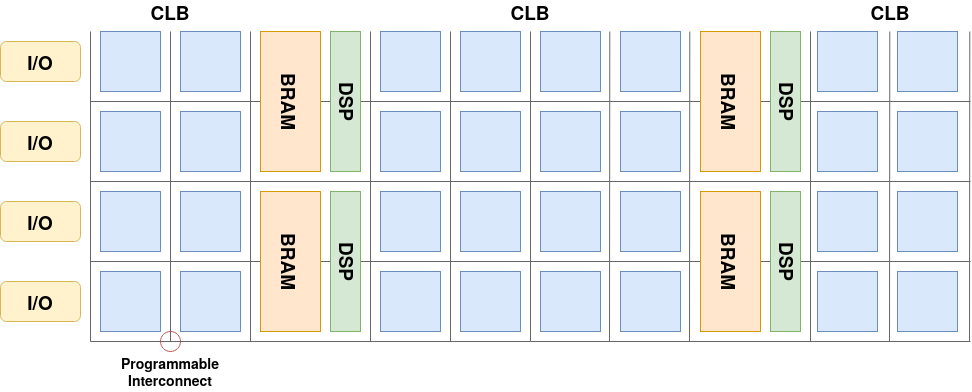
\includegraphics[width=1.0\textwidth]{Figures/FPGA-Structure.png}
                \caption[Xilinx Virtex 7 FPGAs structure]{Simplified schematic of Xilinx Virtex 7 FPGAs structure}
                \label{ch.problem:sec.hardware:ssec.fpga:sssec.fpga:fig.structure}
            \end{figure}
            \begin{figure}[h!]
                \centering
                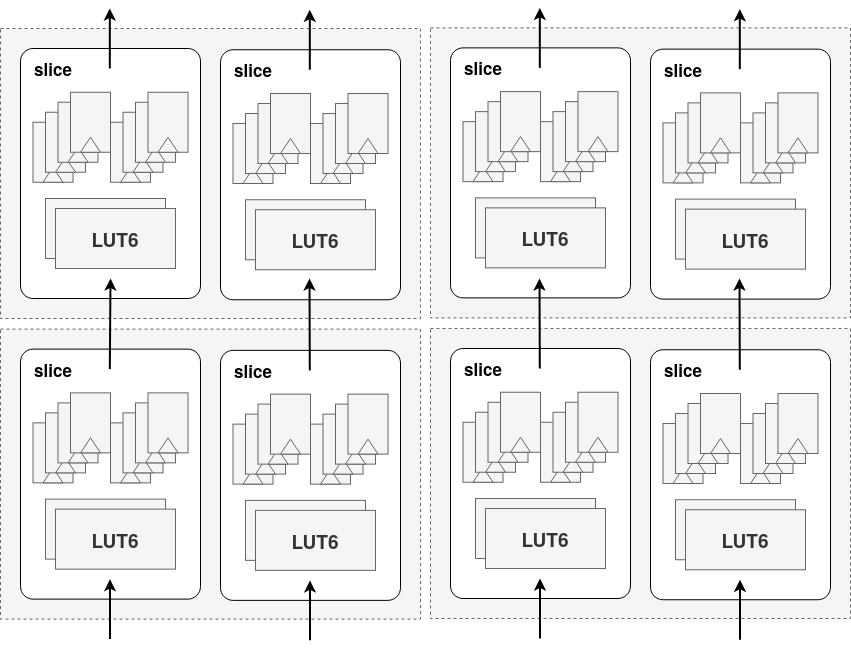
\includegraphics[width=0.8\textwidth]{Figures/FPGA-CLB.png}
                \caption[Xilinx Configurable Logic Blocks]{\myLongAcs{CLB}{Configurable Logic Block}: Xilinx FPGAs basic blocks}
                \label{ch.problem:sec.hardware:ssec.fpga:sssec.fpga:fig.clb}
            \end{figure}

            In order to build efficient design methodologies for \myAc{FPGA} based accelerators, one must understand board structures to comprehend technological specificities.
            Figure \ref{ch.problem:sec.hardware:ssec.fpga:sssec.fpga:fig.structure} introduce a simplified structure of a Xilinx \myAc{FPGA} as an example.
            As can be remarked, the structure is inherently heterogeneous, area being distributed between \myLongAcs{IO}{Input/Output block}, \myLongAcs{CLB}{Configurable Logic Block}, \myLongAcs{DSP}{Digital Signal Processor} and \myLongAcs{BRAM}{Block RAM}.
            Digital functions are based on \myAcs{CLB} (Fig. \ref{ch.problem:sec.hardware:ssec.fpga:sssec.fpga:fig.clb}, as defined in \cite{xilinx_clb_2016}) that include both computation resources with \myLongAcs{LUT}{Look-Up Table} and memory resources with \myLongAcs{FF}{Flip Flop}, but \myAc{DSP} blocks can be used to perform specific computations like multiplications, and \myAc{BRAM} can be used as embedded memory to offer large memories with low access latency.
            At least four different resources are thus to be considered when developing a hardware accelerator for such target --- \myAc{LUT}, \myAc{FF}, \myAc{DSP} and \myAc{BRAM} --- depending on both objectives and constraints of the problem.

            Nowadays, most of \myAcs{FPGA} are integrated in various \myLongAcs{SoC}{Systems on Chip}, tightly coupled with \myAcs{CPU} and other peripherals.
            However, in the context of this work, we will only consider \myAc{FPGA} implementation of different algorithms, and try to ease the life of \myAc{FPGA} developers, with no further focus on the integration of the accelerators.

            Such considerations raise the first interrogations of this manuscript: 
            \mdr{
                \begin{itemize}
                    \item How can we ease hardware development ?
                    \item How can we integrate \myAcs{FPGA} specific constraints in hardware\\design methodologies ?
                \end{itemize}
            }

    \subsection{Standard Paradigms}
    \label{ch.problem:sec.hardware:ssec.paradigms}
        As circuit complexity (\ie number of transistors used in a chip) is growing exponentially, as stated by {\bf Gordon Moore's law} in 1965 \cite{moore_cramming_1965}, hardware designs methodology are bound to evolve and exhibit high level abstraction to developers to cope with the scaling of \myLongAc{VLSI}{Very Large Scale Integration}. 

        First languages developed to describe hardware circuits by abstracting low level considerations were \myLongAcs{HDL}{Hardware Description Language} such as VHDL and Verilog.
        Originally developed for hardware simulation, working at \myLongAc{RTL}{Register-Transfer Level} --- \ie considering data signal as entity instead of considering physical implementation details such as transistor layout and power supply --- their aim was to raise the abstraction level and allow design of large scale circuits.
        To do so, they allow to describe complex circuits by combining behavioural descriptions (how digital signals are behaving in the circuit, often used to describe basic modules with simple functionalities), and structural descriptions (how are basic blocks interacting).
        \myAc{HDL} classic development processes are quite straightforward, as can be seen in Figure \ref{ch.problem:sec.hardware:ssec.paradigms:fig.rtl} (as translated from Prost-Boucle's thesis \cite{prost-boucle_generation_2014}), consisting in manual translations of sequential algorithm to hardware description of the functionality.
        Circuit descriptions are then fed to a set of time consuming software --- including {\bf synthesis} and {\bf place and route} steps --- in order to translate such high level descriptions to physical representations that can be used to program \myAcs{FPGA}.
        Moreover, in order to comply with design constraints and objectives, such process requires manual iterations to find an acceptable fit, and each iteration can be expensive due to the complexity of both synthesis and place and route processes, and may require manual modifications of the original design, which can be both time consuming and error prone tasks.
        
        \begin{figure}[h!]
            \centering
            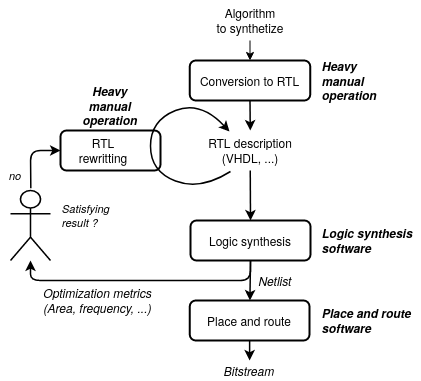
\includegraphics[width=0.8\textwidth]{Figures/HDL-flow.png}
            \caption{Example of RTL design flow}
            \label{ch.problem:sec.hardware:ssec.paradigms:fig.rtl}
        \end{figure}

        \newpage
        Another approach for easing hardware development is based on \myLongAcs{DSL}{Domain Specific Language}.
        \myAcs{DSL} are languages leveraging prior knowledge about the application domains (what are the important operations to perform, what data patterns are frequently used, ... \ie what domain specific optimizations can be performed) to build efficient mapping for acceleration.
        In this way, this approach differs from \myAc{DSP} usage, as the goal is not to program specific processors but rather build generic circuits --- \eg on \myAc{ASIC} or \myAc{FPGA} --- using specificity of a particular domain.
        A typical \myAc{DSL} development flow (quite similar to \myAc{HDL} ones) is presented in Figure \ref{ch.problem:sec.hardware:ssec.paradigms:fig.dsl}. 
        Using domain specific knowledge allow easier writing and refinement of the \myAc{DSL} code base, compared to \myAc{HDL} programming, resulting in faster iteration steps, and feedback generations can also be enhanced by using pre-synthesis estimations based on \myAc{DSL} operations, producing faster development methodologies.
        In fact, providing early estimations of iteration metrics --- \eg area and frequency --- is a common technique to accelerate development flows by reducing the time dedicated to synthesis and place and route steps, and it was used as used as a basis of one of the main initiatives for easier development: \myLongAc{HLS}{High Level Synthesis}.
        \begin{figure}[h!]
            \centering
            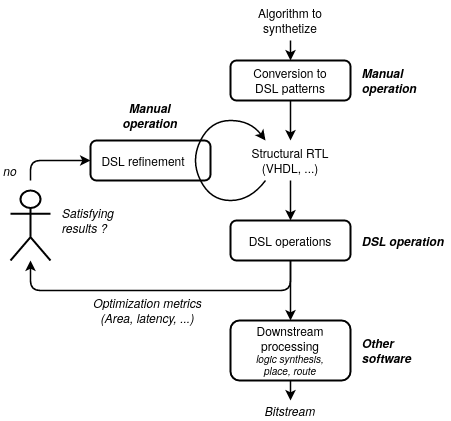
\includegraphics[width=0.8\textwidth]{Figures/DSL-flow.png}
            \caption{Example of DSL design flow}
            \label{ch.problem:sec.hardware:ssec.paradigms:fig.dsl}
        \end{figure}

        \myAc{HLS} methodologies have been developed to close the gap between software developers and hardware designers.
        It is based on a modification of the entry point of the whole process, as it does no longer require to use hardware specific languages such as \myAcs{HDL} or \myAcs{DSL}, but rather uses standard software languages such as {\bf C language} to describe the target algorithm, and then relies on a translation tool that compiles this algorithmic approach to a hardware description at \myAc{RTL} level.
        Figure \ref{ch.problem:sec.hardware:ssec.paradigms:fig.hls} (also translated from Prost-Boucle's thesis \cite{prost-boucle_generation_2014}) introduces a classical \myAc{HLS} based design flow, operating on an intermediate representation issued from the compilation of the input algorithm to perform optimization-estimation steps until given constraints and objectives are respected.
        Manual interventions of the developer are reduced as the software is able to modify the generated circuits in order to optimize the design, but can be needed in order to guide the tool by adding specific knowledge --- using optimization directives (such as {\bf C pragmas}) directly in the algorithm description to define memory patterns or exhibit parallelism for example.
        This feature allows to close the performance gap with \myAc{HDL} design flows, but as it requires specific hardware knowledge, it can no longer directly be used by software neophytes and require prior skill improvement.
        
        \begin{figure}[h!]
            \centering
            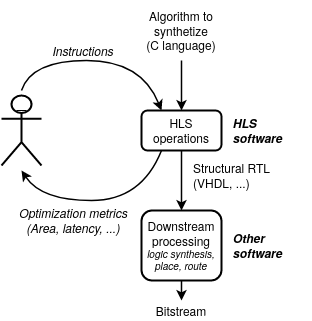
\includegraphics[width=0.68\textwidth]{Figures/HLS-flow.png}
            \caption{Example of HLS design flow}
            \label{ch.problem:sec.hardware:ssec.paradigms:fig.hls}
        \end{figure}

        A quick review of standard paradigms for hardware development hence exhibits some interrogations about classical design methodologies:
        \mdr{
            \begin{itemize}
                \item What are the strength of standard paradigms for hardware\\development ?
                \item What are their limitations ?
                \item How can we ease hardware development processes ?
            \end{itemize}
        }

    \subsection[Hardware Construction Languages]{Addressing Standard Paradigms Limitations through {\it Hardware Construction Languages}}
    \label{ch.problem:sec.hardware:ssec.hcl}
        Standard paradigms for hardware development have evolved the last decade in order to cope with the needs of faster development methodologies and close the gap with software processes.
        However, such methodologies present limitations that one should try to overcome in order to ease the life of hardware developers.
        \myAc{HDL} development requires time consuming and error prone processes, and does not allow easy component re utilization, as evolving a design for a new use case require heavy manual modification of the base code. 
        On the other hand, \myAc{HLS} methodologies can accelerate development processes, and code re utilization is easier as the base code is lighter than with \myAcs{HDL} --- nonetheless, modifying an existing accelerator requires an advanced knowledge of inserted directives which may not be intuitive, and the whole process relies on automatic tool inferences.
        Algorithmic compilation toward hardware description is a difficult problem, as it implies a change of paradigm, from a sequential representation of the algorithm toward a behavioural definition of a circuit. 
        In order to do so, the tool is taking decision that are usually taken by expert developers in standard \myAc{HDL} methodologies that may generate non optimal designs, and wrong directive usage may accentuate this flaw.
        Moreover, with the growing need of performance and efficiency, some of those decisions may be very specific to produce optimal utilization of available resources, and programming languages should allow developers to have full control over generated hardware --- and it cannot be done if automatic decisions are taken without the user knowing it.
        In fact, \myAc{HLS} enables higher abstraction of circuits for design processes, but results in a lack of control over how those circuits are generated.
        As for \myAcs{DSL}, their usage is by-design limited to specific domains, and thus cannot be generalized as hardware development methodologies.

        To cope with those problems and improve the expressivity of developers while maintaining control over generated hardware, new paradigms are emerging, with \myLongAcs{HCL}{Hardware Construction Language} among them.

        \myAcs{HCL} are based on high level languages, allowing to build hardware generators instead of hardware circuits: instead of building a specific accelerators for a given task, such as a digital \myLongAc{FIR Filter}{Finite Impulse Response Filter} with 128 taps operating with 32 bits fixed point numbers, it can be used to build a parametrized \myAc{FIR Filter} generator that can be used to build various circuits, varying on the number of taps or the data type used for example. 
        To do so, they leverage high level features such as \myLongAc{OOP}{Object-Oriented Programming}, functional programming or reflexivity in order to provide more generic and reusable representations for hardware circuits.
        Moreover, as \myAcs{HCL} are working at \myAc{RTL} like standard \myAcs{HDL}, no performance/area overhead is introduced from using \myAc{HCL} over any other \myAc{HDL} \cite{izraelevitz_2017_reusability}, resulting in controllable generation of hardware implementations.
        Figure \ref{ch.problem:sec.hardware:ssec.paradigms:fig.hcl} represents a typical \myAc{HCL} development flow, where the main difference with respect to standard paradigms is that both generator description and parameters definition are exposed by users, allowing to manage generated circuits while easing reuse and iteration over generated designs through exposed programming features.

        \myAcs{HCL} relies on \myLongAcs{HCF}{Hardware Construction Framework} to translate target-independent \myAc{RTL} code to technology dependent \myAc{RTL}, leveraging a compiler-like separation of concerns: using an \myLongAc{IR}{Intermediate Representation} of circuits to perform optimization and code generation, target specific concerns are decorrelated from \myAc{HCL} description as they can be managed directly by operating on the \myAc{IR}.
        Common \myAcs{HCL} use high level languages such as \scala{} for \myLongAc{Chisel}{Constructing Hardware in a Scala Embedded Language} \cite{bachrach_chisel_2012}, {\bf python} for PyMTL \cite{lockhart_pymtl_2014} or {\bf Haskell} for C$\lambda$ash \cite{baaij_clash_2010}.

        As \chisel{} is a promising \myAc{HCL}, with state of the art implementations from both academic and industrial worlds, such as in-order and out-of-order RISC-V implementations \cite{celio_berkeley_2015} \cite{asanovic_rocket_2016} or Google latest \myLongAc{TPU}{Tensor Processing Unit} \cite{google_tpu_2018}, it will be used as an example of \myAc{HCL} in this work.
        \chisel{} development flow is quite similar to standard \myAc{HDL} flows as it relies on the same tool set to generate both constraint and objective metrics and resulting bitstream --- in fact \chisel{} is integrated in standard \myAc{HDL} flows by generating structural \myAc{RTL} (\tn{Verilog}) code after what is called the emission phase (\ie building a non parametrized hardware circuit from the corresponding hardware generator).
        However, as both hardware generator notion and high level programming features for hardware development are recent progresses, improvements of \myAc{HCL} based methodologies are still to be proposed.

\clearpage
        \begin{figure}[h!]
            \centering
            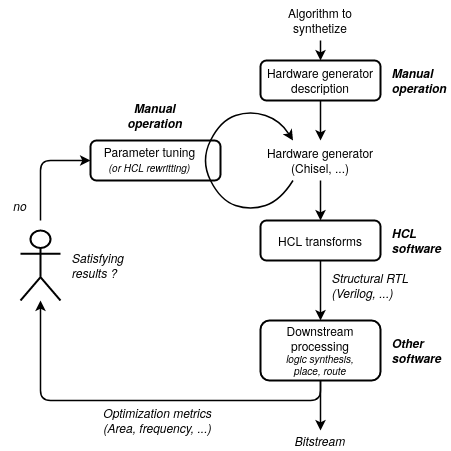
\includegraphics[width=0.83\textwidth]{Figures/HCL-flow.png}
            \caption{Example of HCL design flow}
            \label{ch.problem:sec.hardware:ssec.paradigms:fig.hcl}
        \end{figure}

        Emergence of \myAc{HCL} paradigm hence raises few interrogations on the improvement that new technologies and methodologies can bring to the industry of semi-conductor:
        \mdr{
            \begin{itemize}
                \item How can \myAcs{HCL} cope with standard paradigms limitations ?
                \item How can high level programming features be used in hardware\\development ?
                \item What can \myAcs{HCL} bring to hardware developers ?
                \item How can \myAcs{HCL} flow be improved for easier iterations over generated designs ?
            \end{itemize}
        }

        Moreover, as \chisel{} will be used as a basis for this work, an analysis of its interesting features is provided in Appendix \ref{app.chisel}. It should help readers to understand the opportunities brought by the \myAc{HCL} paradigm, using simple examples of \chisel{} usage to expose differences from standard \myAcs{HDL}.


%%%%%%%%%%%%%%%%%%%%%%%%%%%%%%%%%%%%%%%%%%%%%%%%%%%%%%%%%%%%%%%%%%%%%%%%%%%%%%%%

\clearpage
\section{Design Space Exploration}
\label{ch.problem:sec.dse}

    \subsection{Definitions and Interests}
    \label{ch.problem:sec.dse:ssec.definitions}

    It may seem counter intuitive, but hardware designers expertise is more about decision making than describing circuits.
    As a matter of fact, implementing a particular algorithm for a given target can be done in a lot of different ways, and it is up to the developer to choose among different implementation options to build optimal circuits with respect to its use case.
    However, even with senior expertise, optimal solutions may not be trivial, and developer may not even consider them in the process, resulting in suboptimal designs.
    
    To cope with this problem, \myLongAc{DSE}{Design Space Exploration} methodologies have emerged, allowing exploration and comparison of implementation options at different granularity levels --- options can vary from basic operation implementations such as multiplication algorithm, to global parameters, such as parallelism level of the design.
    A design space is defined as the set of every possible implementation candidate for a given algorithm, and as implementation options may grow exponentially with circuit complexities, exhaustive exploration processes may be unfeasible in an acceptable amount of time.
    Due to that, more complex exploration strategies were built to reduce space traversal, thus reducing exploration time while maintaining satisfying \myLongAc{QoR}{Quality of Results}, \ie finding implementations with performances comparable to a global optimal implementation as could be found from exhaustive space traversal. 

    However, one cannot define a generic, optimal solution for exploration, as a lot of parameters are both target and algorithm specific \cite{schafer_high-level_2020}.
    Moreover, design space definition is not trivial either, as defining the implementation options require either automatic tool inferences, or programming expressivity for developers to bring their expertise in the process.
    Ergo, \myAc{DSE} methodologies remain a prolific search domain, and standard approaches are continuously being improved --- raising even more interrogations:

    \mdr{
        \begin{itemize}
            \item What does \myAc{DSE} bring to hardware developers ?
            \item Which features are necessary for efficient \myAc{DSE} ? 
            \item Which features could be useful ?
        \end{itemize}
    }

\clearpage
    \subsection{Standard Approaches}
    \label{ch.problem:sec.dse:ssec.approaches}

    As exhaustive exploration remains impracticable for complex circuits, more clever exploration strategies were developed to fasten exploration processes. 
    In order to do so, one of the main approach is based on {\bf Pareto optimal solutions} \cite{schafer_high-level_2020}: considering both a performance and a cost metric, Pareto optimal solutions are implementations that are optimal in their neighbourhood, meaning that modifying a parameter will result in either a more costly or a less performant solution.
    The goal is thus to build algorithm to approximate the Pareto frontier without exhaustive traversal of the design space, resulting in optimal design finding in a heavily reduced amount of time.
    Figure \ref{ch.problem:sec.dse:ssec.definitions:fig.pareto} introduce a classical, Pareto based \myAc{DSE} methodology, using resource usage (which can be amount of transistor, of \myAc{LUT}, of \myAc{DSP}, ...) as a cost metric, in order to find best implementations under both resource and performance constraints. 
    It enables design space partitioning to exhibit a reduced number of implementations to developers, helping them in the design process, as they can now choose among a set of implementations with a warranty that they did not miss potentially optimal solutions.

    \begin{figure}[h!]
        \centering
        % includes here
\usetikzlibrary{patterns}

% style here

% figure here
\scalebox{1.25}{
\begin{tikzpicture}
\begin{axis}[
    xlabel={Resources},
    ylabel={Performance},
    axis lines = middle,
    x label style={at={(axis description cs:0.5,-0.01)},anchor=north},
    y label style={at={(axis description cs:-0.01,0.5)},rotate=90,anchor=south},
    xtick distance=1,
    ytick distance=1,
    yticklabels={,,},
    xticklabels={,,},
    xmin=0,xmax=5,
    ymin=0,ymax=5
]

\addplot [name path=curve,mark=none,smooth] coordinates{(1, 5) (1.01, 4.9) (1.1, 4) (1.25,3.2) (1.5,2.5) (2, 1.8) (2.5,1.45) (3, 1.25) (4, 1.07) (4.9, 1.01) (5, 1)};
\draw [name path=resource,red] (4, 0) -- (4, 5*\pgfkeysvalueof{/pgfplots/ymax}/6+0.05) node[right=0.2,rotate=-90] (resnode) {Resource constraint} -- (4, \pgfkeysvalueof{/pgfplots/ymax});
\draw [name path=performance,blue] (0, 3) -- (8*\pgfkeysvalueof{/pgfplots/xmax}/15, 3) node[above=0.1] (perfnode) {Performance constraints} -- (\pgfkeysvalueof{/pgfplots/xmax}, 3);
\addplot[fill=gray]fill between[of=curve and performance,soft clip={domain=1.3:4}];
\node (solution) at (2.85,2.32) {Suitable solutions};
\end{axis}
\end{tikzpicture}
}

        \caption[Pareto frontier representation]{Example of Pareto optimal solutions finding under resource and\\performance constraints}
        \label{ch.problem:sec.dse:ssec.definitions:fig.pareto}
    \end{figure}

    As shown in Figure \ref{ch.problem:sec.hardware:ssec.paradigms:fig.hls}, standard \myAc{HLS} development flows rely on \myAc{HLS} operations over generated circuit in order to generate acceptable solutions with respect to objective and constraints.
    To do so, \myAc{DSE} is used in most \myAc{HLS} tool as a medium to find acceptable solutions, varying implementation parameters from the original algorithm, such as loop unrolling, operation pipelining of memory partitioning: by giving freedom to the tool to make its own decision, a heavy design space is generated to compare a lot of different implementations.
    In order to reduce design space width, most flows thus use algorithms to approximate the Pareto frontier, using specific heuristics such as machine learning \cite{nardi_practical_2019} \cite{ferretti_leveraging_2020} or genetic algorithms \cite{manuel_model-based_2020}, and building efficient exploration strategies remains a trending search topic.
    Moreover, optimization directives can also be given to guide the exploration of the generated design space, resulting in efficient \myAc{DSE} processes.

    However, defining optimization directives requires user expertise, and automatic inferences about the design space and how to explore it may result in a lack of control of generated accelerators, which may lead to the impossibility to find the best fit --- especially on specific targets such as \myAcs{FPGA} where resource heterogeneity requires experience to produce clever decisions.

   Such considerations about standard \myAc{DSE} approaches bring interrogations about such processes:

    \mdr{
        \begin{itemize}
            \item What are the limitations of standard \myAc{DSE} approaches ? 
            \item Can \myAcs{HCL} help addressing those limitations ?
        \end{itemize}
    }

    \subsection{Limitations}
    \label{ch.problem:sec.dse:ssec.limitations}
        While standard \myAc{DSE} approaches have grown mature the last two decades --- especially with the rise of \myAc{HLS} tools --- limitations are still to be addressed to provide generic methodologies appropriate for every possible use cases.

        We discussed the challenge of building an interesting design space to explore, as automatic inferences of the tools used to generate implementation options allow multiple variations to be explored, but might result in an uncontrollable design generation in the end.

        Moreover, doing so, the generated design spaces are composed in a vast majority of known sub optimal solutions, as no particular expertise is used at design space generation step.
        It results in heavy design spaces that cannot be explored exhaustively, with the emergence of exploration strategies such as Pareto approximations to cope with the large amount of possible implementations, even if a lot of those implementations are not sound and would never be considered by a hardware developer.

        Last but not least, most of \myAc{DSE} tools define their own strategies, as well as metrics to optimize in the process, resulting in methodologies that are hard to adapt and reuse to any new use case.
        In fact, some particular use cases require to define specific metrics to optimize and consider, as well as particular exploration strategies, and tools should allow developers to bring their expertise and knowledge to the exploration process definition.
        For example, specific domains such as \myLongAc{AxC}{Approximate Computing} requires to consider the \myLongAc{QoS}{Quality of Service} of circuits in order to provide guarantees about the functionality of a design.
        However, most \myAc{DSE} tools does not allow users to add such metric in the exploration process, resulting in the need to use different flows to consider multiple metrics.

        In this context, one may wonder what can \myAcs{HCL} bring to hardware developers, especially in the context of \myAc{DSE}:
        \mdr{
            \begin{itemize}
                \item What can flexibility and genericity bring to \myAc{DSE} ?
                \item How can users define use case specific metrics ?
                \item How can users build custom exploration strategies ?
                \item How can \myAcs{HCL} be used for efficient \myAc{DSE} ?
            \end{itemize}
        }

%%%%%%%%%%%%%%%%%%%%%%%%%%%%%%%%%%%%%%%%%%%%%%%%%%%%%%%%%%%%%%%%%%%%%%%%%%%%%%%%

\section{Motivations and Organization}
\label{ch.problem:sec.synthesis}

    \subsection{Problem Statement}
    \label{ch.problem:sec.synthesis:ssec.summary}

        This chapter introduces the motivations of the work presented in this thesis.
        We discuss the role of \myAcs{FPGA} in the context of hardware acceleration, and expose various methodologies used to develop hardware accelerators relying on \myAcs{FPGA} specificities.
        Among them, we introduce \myAcs{HCL} as an emerging programming paradigm, and consider their usage to cope with standard paradigm limitations.
        We put a particular focus on \myAc{DSE} processes as a way to increase hardware developer productivity, and discuss \myAcs{HCL} usage to improve those processes.

\clearpage
        With respect to those considerations, the goal of this thesis is hence to answer those questions:
        \lmdr{
            \begin{itemize}
                \item How can \myAc{FPGA} designers productivity be improved\\using \myAcs{HCL} ?
                \item Which limitations of standard paradigms for hardware\\development can be addressed using \myAcs{HCL} ?
                \item How can \myAcs{HCL} be used for efficient \myAc{DSE} on \myAcs{FPGA} ?
            \end{itemize}
        }

    \subsection{Thesis Organization}
    \label{ch.problem:sec.synthesis:ssec.organization}
        In order to provide an intelligible analysis of the usage of \myLongAcs{HCL}{Hardware Construction Language} to build a flexible \myLongAc{DSE}{Design Space Exploration} framework that target \myLongAcs{FPGA}{Field-Programmable Gate Array}, this thesis is organized as follows.

        Chapter \ref{ch.state} outlines the related works of the literature on efficient \myAc{DSE} for \myAcs{FPGA}, as well as their limitations.
        Chapter \ref{ch.estimators} discusses the need of qualitative estimators to increase the developers productivity, and proposes interesting metrics to be considered in design and exploration processes, as well as relevant estimation methodologies to be used.
        Chapter \ref{ch.dse} introduces the usage of \myAc{DSE} in an \myAc{HCL} context, before exhibiting two complementary methodologies to exploit this paradigm in user defined custom strategies.
        In particular, a novel formalism for \myAc{DSE} is introduced in order to exhibit how the functional programming paradigm can be used to build intelligible and concise exploration strategies.
        Chapter \ref{ch.expe} exposes the experimental setup, including a software demonstrator integrating the defined methodologies and a benchmark of representative applications, and presents the results of the experimentations that were led.
        Chapter \ref{ch.conclusion} concludes this manuscript, discussing both the proposed contributions and the perspectives of evolution.

        In addition to those chapters, four appendixes are to be found at the end of this manuscript.
        Among them, Appendix \ref{app.chisel} provides some insights about the usage of \chisel, the chosen \myAc{HCL} for this work, which will help the reader to have a better apprehension of the features that such language can bring to the world of hardware design.

%%%%%%%%%%%%%%%%%%%%%%%%%%%%%%%%%%%%%%%%%%%%%%%%%%%%%%%%%%%%%%%%%%%%%%%%%%%%%%%%
%%%%%%%%%%%%%%%%%%%%%%%%%%%%%%%%%%%%%%%%%%%%%%%%%%%%%%%%%%%%%%%%%%%%%%%%%%%%%%%%

\cleardoublepage
%-------------------------------------------------------------------------------
\chapter{State of the Art}
\labelchapter{ch.state}
%-------------------------------------------------------------------------------

%%%%%%%%%%%%%%%%%%%%%%%%%%%%%%%%%%%%%%%%%%%%%%%%%%%%%%%%%%%%%%%%%%%%%%%%%%%%%%%%
%%%%%%%%%%%%%%%%%%%%%%%%%%%%%%%%%%%%%%%%%%%%%%%%%%%%%%%%%%%%%%%%%%%%%%%%%%%%%%%%

% \vspace{-0.8cm}
\lettrine[lines=2]{T}{his} chapter outlines the related works about \myLongAc{DSE}{Design Space Exploration} on \myLongAc{FPGA}{Field-Programmable Gate Array}.
As the notion of \myAc{DSE} can refer to any process exploring variations of implementations, it can be applied at various levels of granularity, from basic operator implementations \cite{rehman_architectural-space_2016}\cite{geng_high-speed_2021} to whole \myLongAc{SoC}{Systems-on-chip} \cite{ascia_ga-based_2004}\cite{calborean_automatic_2010}, and can even be applied for software/hardware co design \cite{barone_multi-objective_2021}.

Moreover, when it comes to digital design, \myAc{DSE} processes can be applied for both \myLongAc{ASIC}{Application-Specific Integrated Circuit} and \myAc{FPGA} circuits, and some previous works showed that an optimal \myAc{ASIC} solution may prove to be suboptimal when targeting a \myAc{FPGA} \cite{liu2019accelerating}.

In the context of this work, we will hence focus on \myAc{DSE} application at {\bf kernel level}, meaning that we will consider \myAc{FPGA}-based implementations of more or less complex algorithms that fit on a single \myAc{FPGA} device.

We will start by exposing some popular tools leveraging \myAc{DSE} for \myAc{FPGA} based designs, and will consider how are design spaces exposed in the state of the art methodologies.
We will then examine which metrics are used in \myAc{DSE} processes, and how relevant estimators are built and integrated in the exploration frameworks.
Finally, we will discuss various exploration strategies, along with both their advantages and their limitations, before providing a synthesis of the approaches for \myAc{FPGA}-based \myAc{DSE} in the literature.

\clearpage
\vspace*{\fill}
% \clearpage
%Content section
\minitoc 
\vspace*{\fill}
% \mtcskip 
% \minilof

\newpage
%%%%%%%%%%%%%%%%%%%%%%%%%%%%%%%%%%%%%%%%%%%%%%%%%%%%%%%%%%%%%%%%%%%%%%%%%%%%%%%%

\section{Overview of the Existing Tools}
\label{ch.state:seq.tools}

As an exhaustive listing of every \myLongAc{DSE}{Design Space Exploration} framework is both unfeasible and of limited utility, we will start by providing a brief review of the most popular tools aimed at easing the developers life, focusing on rising the abstraction of design processes with approaches such as \myLongAc{HLS}{High Level Synthesis} and \myLongAcs{DSL}{Domain Specific Language}.

To begin with, Windh \etal{} \cite{windh_high-level_2015} provide a rapid study of high level tools for reconfigurable computing.
A particular focus is put on \myAc{HLS} initiatives, with two industrial tools, namely Xilinx Vivado HLS \cite{zhang_autopilot_2008}\cite{xilinx_vivado_2021} and Altera OpenCL \cite{singh2011implementing}, and two academic frameworks, LegUp \cite{canis2011legup} and ROCCC \cite{villarreal_designing_2010}. 
BlueSpec System Verilog \cite{nikhil2008bluespec}, another approach based on a simplified behavioural model --- abstracting some of the difficulties of standard \myLongAcs{HDL}{Hardware Description Language} --- is also introduced.

Whereas the \myAc{HLS} approach is a main trend toward higher productivity, some \myAc{DSL} based initiatives are also considered to close the gap between domain specialists --- such as data scientists or signal processing experts --- on one hand, and \myAc{FPGA} developers on the other.
Kapre \etal{} \cite{kapre_survey_2016} expose a brief survey of different \myAcs{DSL} and their application domains: while DFiant \cite{port_dfiant_2017} focuses on dataflow based applications, Sano \cite{sano_dsl-based_2015} proposes a framework targeting parallel streaming architectures. 
Kristien \etal{} \cite{kristien_high-level_2019} expose how the \texttt{Lift} framework can be used for efficient design, leveraging functional patterns for compilation, while Spatial \cite{koeplinger_spatial_2018} exhibits \myAc{FPGA} specific patterns and constructs for accelerator generation.

All those initiatives demonstrates the variability of the approaches for efficient design, where the abstraction level, the parametrization, the application domain or the target technology are as many knobs that can be tuned to build an efficient design framework.
Most of those approaches rely --- more or less heavily --- on \myAc{DSE} processes to help designers make expertise-based decisions, such as parallelism exhibition, interface definition or dataflow pipelining.

In order to provide an interesting analysis of the existing literature on \myAc{FPGA} based \myAc{DSE}, we thus chose to focus on three main concerns, which we identified as being key levers for efficient strategy definition: 
{\setstretch{0.9}
\begin{itemize}
    \item {\bf design space exposition} --- \ie defining which implementation variations can be explored, and how to generate corresponding architectures
    \item {\bf metric definition} --- \ie exposing metrics of interests for a given use-case, as well as how to build and integrate estimators
    \item {\bf exploration algorithm} --- \ie describing how to scan the design space in a clever way, providing rapid yet accurate results
\end{itemize}
}

\clearpage
\section{Design Space Exposition}
\label{ch.state:sec.space}
    When building a \myAc{DSE} framework, one of the main concerns is to define which variations are to be considered in the exploration, and how to generate the corresponding implementations from the initial description.

    Various abstraction levels are also to be considered, ranging from high level programming languages such as python or C/C++, which can be used to allow software developers to design their own circuits, to \myLongAc{RTL}{Register-Transfer Level} languages, which enable hardware designers to efficiently control the built accelerators based on their expertise.

    However, the input language and the abstraction level can also be considered from another point of view: the level of control over the implementation variations.
    The \myAc{DSE} methodologies can either rely on the explicitation of generation parameters, or on the automatic inference of the implementation variations --- but most of the popular high level tools are based on a mix-up of those two options, allowing users to define some variations while inferring others, based on the standard design methodology (with potential optimizations linked to the application domain and/or the target board).

    In this section, we will hence consider how the design variations are chosen in the different approaches, rather than their abstraction levels.
    Doing so allows to classify the \myAc{DSE} initiatives without introducing the classical distinction between \myAc{HLS}, \myAc{DSL} and other techniques, as the main difference when it comes to exploration is the way to expose the explored design space.

    \subsection{Explicit Parametrization}
    \label{ch.state:sec.space:ssec.explicit}
        
        The basic idea of the explicit parametrization approach is to allow users to define explicit parameters in their code, in order to provide an explorable design space built over understandable variations.
        Such parameters can be application specific, for example matrix dimensions in a matrix multiplication kernel, or independent, with standard parameters such as the \myLongAc{IO}{Input/Output} bandwidth or the element type \cite{ferres_2021_integrating}.

        Application specific generators have been introduced in the literature to easily expose and explore design spaces, at various levels of granularity.
        While Rehman \etal{} \cite{rehman_architectural-space_2016} use a library of basic blocks and the composition of components to explore approximate multiplier implementations, Yiannacouras \etal{} \cite{yiannacouras_exploration_2007} introduce SPREE (Soft Processor Rapid Exploration Environment), a framework allowing to explore the variations of a processor by leveraging standard \myAc{CPU} notions such as \myLongAc{FU}{Functional Unit} implementation and dataflow pipelining.
        Other initiatives have been proposed for domain specific \myAc{DSE}, such as the implementation of \myLongAcs{CNN}{Convolutional Neural Network}, for example using different dataflow techniques as variations \cite{park_roofline-model-based_2020}.
        We can thus state that developers may need to expose very specific parameters in their exploration flow, and the exploration frameworks should provide a way to do so.

        To easily integrate the definition of parameters into the standard design flows, Paletti \etal{} \cite{paletti_dovado_2021} provide {\bf Dovado}, a \myAc{RTL}-based exploration framework leveraging \myAc{HDL} {\it generic} features to build the design space.
        However, their perspectives include supporting other languages with more convenient ways for parametrization, such as \chisel{} or other \myAcs{HCL}.

        \myAcs{HCL} are recent initiatives focused on building parametrizable generators instead of use-case specific accelerators, using high level languages as entry points to leverage promising software paradigms in the hardware world.
        Among them, we can list \python{} based initiatives such as {\bf MyHDL} \cite{jaic2015enhancing} or {\bf PyMTL} \cite{lockhart_pymtl_2014}, \scala{} based frameworks such as \chisel{} \cite{bachrach_chisel_2012} and {\bf SpinalHDL} \cite{papon2017spinalhdl}, and {\bf C$\lambda$ash}, an \haskell{} based project \cite{baaij_clash_2010}.

        Several \chisel{} based initiatives are exploring the possibilities of both high level programming features and highly parametrizable constructors to provide interesting exploration features.
        Cook \etal{} \cite{cook_diplomatic_2017} proposed {\bf Diplomacy}, a parameter negotiation framework to automatically select and propagate generation parameters of the {\bf Rocket chip} processor\footnote{Rocket-chip is an open-source, in-order version of a \chisel{}-based RISC-V processor.} \cite{asanovic_rocket_2016}. 
        To go further, Bai \etal{} introduced the {\bf BOOM-Explorer} \cite{bai_boom-explorer_2021} to explore the \myLongAc{BOOM}{Berkeley Out-of-Order Machine} core\footnote{\myAc{BOOM} is an out-of-order implementation of a \chisel{}-based RISC-V core.}, varying the generation parameters of the different pipeline stages in the dataflow.
        A more generic approach was also provided with {\bf JackHammer} \cite{schmidt_fast_2015}, an exploration framework for \chisel{} based designs.
        However, the initiative is not maintained anymore, and is claimed to be too specific for SHA-3, the target algorithm.

        As one can observe here, exposing explicit parameters through \myAc{HCL} usage seems to be a promising way for an efficient \myAc{DSE} framework definition. 
        Moreover, as \chisel{} is used as a basis for this work, we provide some useful insights and basics in Appendix \ref{app.chisel}, that should help readers to be more familiar with the possibilities that this language offer.

	% \Olivier{Il faut surement dire dans cette section que tous les outils de HLS permettent via des pragmas ou des fichiers de directives de piloter explicitement la génération de l'architecture}
    \subsection{Implicit Inferences}
    \label{ch.state:sec.space:ssec.implicit}

        While a generator-based exploration allows users to define which variations are to be explored, it cannot be used in frameworks based on a change of programming paradigm, such as \myAc{HLS}.
        As \myAc{HLS} is based on translating an algorithmic description to a hardware one, choices are to be taken to model the decisions that a hardware developer would take when doing the same task --- \eg the level of loop unrolling, the memory model or the input bit width.
        While those choices would usually require a lot of parameters and description to be efficient, standard \myAc{HLS} tools often automatically infer which transformations are to be triggered to provide an efficient solution.

        To do so, the \myAc{HLS} flows iteratively select which transforms to perform over the \myLongAc{IR}{Intermediate Representation}, optimizing a certain set of objective functions under constraints \cite{prost-boucle_fast_2014} --- Ye \etal{} \cite{ye_scalehls_2021} even consider a multi-level \myAc{IR} to expose different optimizations depending on the abstraction level.
        Some \myAc{DSL} also use a similar approach for compilation: the {\tt Lift} \cite{kristien_high-level_2019} frameworks expose implementation variations using rewrite rules over the original description, while Sano \etal{} \cite{sano_dsl-based_2015} exploit the inherent parallelism to generate different implementations to be explored.

	% \Olivier{Le calcul approximatif a clairement sa place dans ton état de l'art, mais est-ce vraiment de l'explo implicite dans ces papiers.}
        A similar approach is also used in \myLongAc{AxC}{Approximate Computing} based exploration frameworks, as the actual implementation of used operators does not really matter.
        As a result, different approximations are considered to generate the implementations (named {\it variants} by Witschen \etal{} \cite{witschen_circa_2019}) and build the design space \cite{manuel_model-based_2020}\cite{barone_multi-objective_2021}.
        Other initiatives consider some optimizations that are possible due to the \myAc{AxC} inherent freedom, such as optimizing the data word lengths to reduce required hardware \cite{herve_data_2005} or reordering the floating-point operations to optimize latency \cite{gao_automatically_2016}.

        Those approaches thus bypass both explicit decisions and parameter definition that should be provided by user, and automatically infer how to transform the circuit representation to provide a best fit --- which may result in non optimal designs (with respect to a manually tuned design), and does not allow to fully control generated circuits.

    \subsection{Mixing-up Approaches}
    \label{ch.state:sec.space:ssec.mixing}
        However, when looking to the most popular \myAc{DSE} flows, we can remark that they are actually based on a mix-up of those two approaches.

        To begin with, Schafer \etal{} \cite{schafer_high-level_2020} provide a comprehensive study of the \myAc{HLS} approaches for \myAc{DSE}, and formalize a notion that is key in the design space exposition process: {\bf exploration knobs}.
        Knobs are design parameters exposed at some point in the process, that allow the users to consider the synthesis process as a {\it black box} --- providing different knobs as inputs of the process resulting in a different \myAc{RTL} implementation at the end of it.
        They are classified in three different categories, that are mainly relevant for \myLongAc{ASIC}{Application-Specific Integrated Circuit} design, but can also be considered when targeting a \myAc{FPGA} implementation:

\clearpage

        \begin{itemize}
            \item {\it local synthesis directives}, which are used to control the local inferences of the \myAc{HLS} tool.

                They are often implemented using {\it pragmas} that are directly integrated in the entry code, in order to fix some parameters that would have been inferred by the tool otherwise --- leveraging user expertise.
            \item {\it global synthesis directives}, which are used to specify some global parameters for the synthesis.

                Among them, we can find the scheduling algorithm to be used for compilation, the clock constraints or the \myLongAc{FSM}{Finite State Machine} encoding scheme.
            \item {\it \myAc{FU} constraints}, which defines the level of sharing of \myAcs{FU}, introducing a performance/area trade-off.

                Such knob is often not considered by \myAc{FPGA} targeting \myAc{HLS} tools, as sharing a \myAc{FU} on \myAc{FPGA} often requires more resources (mainly muxes) than implementing another computation unit.% \cite{schafer_high-level_2020}.
        \end{itemize}

        The popular \myAc{HLS} tools mainly leverage {\it local synthesis directives}, as it allows to finely control generated hardware.
        However, defining such {\it pragmas} is often a tedious task, as their impact on the generated circuit is often difficult to understand and may vary depending on the compiler version, which requires an expertise about both hardware development and used \myAc{HLS} flow.
        Moreover, it is difficult to modify the base code, as reusing the behavioural description in another context will probably require to tune every {\it pragmas} again, to guide the exploration flow.

        Another approach based on controllable yet automatic inferences as been introduced in {\bf Spatial} \cite{koeplinger_spatial_2018}, where automatic inferences for scheduling and pipelining coexist with user defined parameters for generation.

    \subsection{Exposing an Explorable Design Space}

        We remark that exposing an interesting design space to be explored --- \ie a design space that consider potentially optimal designs for the current use case while providing a structure enabling an efficient exploration --- often requires the developers to bring their expertise using custom parameters, while some freedom can be left to the tool for simple optimizations in order to allow compact but usable descriptions.

        In this way, we consider building an \myLongAc{HCF}{Hardware Construction Framework} based approach for \myAc{DSE}, to allow users to expose specific parameters for the exploration, while allowing automatic transforms --- which should be easily configurable --- to be performed before generation.

\clearpage
\section{Metric Definition and Estimations}
\label{ch.state:sec.metric}
    Another important concern when it comes to \myAc{DSE} is how to define the {\bf goal} of the exploration.
    As stated by Schafer \etal{} \cite{schafer_high-level_2020}, no generic exploration strategy can be defined as it depends on a lot of parameters such as the application specificities, the target, the functioning conditions or the use-case constraints and objectives.
    An exploration process is thus to be defined specifically for a given combination of those parameters, including the objective function(s) to be optimized through the flow --- as a matter of fact, multiple objectives and/or constraints are often to be considered in such processes to provide usable solutions.
    Barone \etal{} \cite{barone_multi-objective_2021} introduce the need for efficient \myLongAc{MOP}{Multi-objective Optimization Problem} solving --- \ie "finding, for some {\it decision variables}, a set of values satisfying {\it imposed constraints}, while optimizing a set of {\it objective functions}" \cite{osyczka1985multicriteria}.

    In this context, we hence aim at providing some insights about interesting metrics and corresponding estimation methodologies for \myAc{DSE}: in other terms, we want to discuss how two implementations can be compared for a given set of constraint(s) and objective(s).
    Two complementary notions will be considered in this section: {\bf metric definition}, which corresponds to circuit properties that hardware developers consider when iterating over their designs, and {\bf estimation methodologies}, which are the ways those metrics are estimated in the flow.

    Actually, to be able to efficiently explore a design space, an {\bf accuracy} {\it vs} {\bf speed} trade-off is introduced in the process, as providing an accurate estimation of a metric may require long procedures from specific tools --- \eg vendor frameworks such as \vivado{} or \quartus{} --- while quick estimation methodologies often result in approximate estimations.
    We will thus consider mainstream metrics for exploration process, as well as interesting methodologies for their estimations, in order to provide users with a way to comprehend and take the best of this trade-off in their \myAc{DSE} design.
    % \needed{Small intro about how to define the metrics, which are commons, which are usefull}
    
    \subsection{Estimating Temporal and Spatial Concerns}
    \label{ch.state:sec.metric:ssec.resource}
        In standard \myAc{FPGA} processes, developers mainly consider two concerns for validating a circuit --- that it fits the target board, and that the temporal behaviour respects the performance constraints.

        The temporal behaviour is mainly considered using {\bf two metrics}: {\bf functioning frequency}, which defines the clock cycle duration for the design, and {\bf latency}, which is an abstract notion considering the number of cycles needed for a computation (\eg{} in stream based applications such as \myLongAc{FIR Filter}{Finite Impulse Response Filter}, it can be defined as the number of cycles needed for an input sample to have an impact on the kernel output).
        It can also be defined by combining those two metrics, providing a global latency metric in second.

        On the other hand, the spatial part is mainly divided in {\bf four metrics} for \myAc{FPGA} design, corresponding to the basic elements of a \myAc{FPGA} structure:
        \begin{itemize}
            \item \myLongAcs{LUT}{Look-Up Table}%, which are the basic blocks for logic operation implementation
            \item \myLongAcs{FF}{Flip Flop}%, which are basic memory elements used for register implementation
            \item \myLongAcs{DSP}{Digital Signal Processor}%, which are dedicated \myAcs{FU} for specific operations such as multiplication
            \item embedded memories, such as \myLongAcs{BRAM}{Block RAM}%, which are wider memory elements
        \end{itemize}

        Estimations for both metrics are classically based on manual analysis of vendor synthesis or implementation reports, which can hence be used as the {\bf reference value} to achieve through estimations, but is obtained after long processes.
        We will hence discuss different levels of estimations, from high abstraction level to \myAc{RTL} based methodology, to provide insights about speed, accuracy and usability of different methodologies.

        \subsubsection{Resource Estimation} 
            To begin with, resource estimation is a key feature for efficient exploration, with various level approaches proposed the last decades.

            As \myAc{RTL} approaches are easy to integrate in any design flow (the representation level being the entry point of most synthesis flows), \myAc{HDL} based methodologies have been proposed for resource estimation.
            They mainly rely on two complementary approaches: modelling steps that the synthesis is expected to take in order to provide realistic estimations \cite{schumacher_fast_2008}, and use characterisation of basic blocks and \myLongAc{IP}{Intellectual Property} cores \cite{deng_accurate_2008}.
            This characterization approach allows to adapt estimators to a given \myAc{FPGA} and synthesis flow by providing a target specific way to generate the basis of the estimation methodology --- to do so, basic blocks of interests are identified and synthesized only once, the report being parsed to provide a characterized model of the component to be used each time a similar component is identified in the estimated circuit.

            As for higher abstraction initiatives, {\bf MATLAB} based approaches have been introduced for early estimation of resource from algorithmic description through analytical models of circuits \cite{nayak_accurate_2002}\cite{hutchison_system_2004} --- however, as \myAc{HLS} initiatives mostly consider C/C++ implementations, approaches based on such model have been left aside for more integrated solutions.

\clearpage
            Regarding \myAc{HLS} recent initiatives, different techniques have been used in order to provide quick feedback to the exploration flow, either based on analytical models --- \eg to estimate \myAc{DSP} usage for multiplication implementation \cite{aung_rapid_2015}, \myAc{BRAM} usage \cite{zhao_performance_2020} or approximate arithmetic implementation \cite{castro-godinez_axhls_2020} --- or on statistical approaches to infer resource usage from a circuit model \cite{meeuws_quipu_2013}.

            Some application specific initiatives have also been proposed, for example using a mathematical model to estimate the resource usage of a \myAc{FPGA}-based \myLongAcs{NoC}{Network-on-Chip} through a learning model \cite{fresse2014mathematical}.

         \subsubsection{Timing Estimation}
            When it comes to early timing estimation, two main approaches are to be considered: either try to estimate the functioning frequency, or fix it using synthesis directives, and use scheduling algorithms to provide a latency estimation.

            While this first approach is closer to standard design flows, it is impracticable to estimate critical path delay at early stages of \myAc{FPGA} based flows, as most of the delay is actually induced by the {\bf routing phase} --- more than 60\% of the delay \cite{xu_area_1996} --- that happens late in the process, is really difficult to model and is heavily target dependent.

            As a result, most of the \myAc{HLS} methodologies rely on the second approach, which is more feasible, is a better fit due to the change of paradigm, and can use the literature on scheduling methods to provide efficient ways to use allocated hardware \cite{prost-boucle_fast_2014}\cite{rincon_technique_2020}.

            In contrast with such static approaches, recent initiatives based on dynamic execution have been proposed to extract sub traces from C/C++ runs, using a {\bf Resource constrained List-Based Scheduler} for latency estimation \cite{zhong_lin-analyzer_2016}\cite{siracusa_comprehensive_2021}.
            The profiling approach provides an interesting alternative to static analysis of the circuit, as the entry point is an executable description of the target algorithm \cite{oneal_hlspredict_2018}.

        \subsubsection{Joint Estimation}
            While we considered separated estimations of both concerns until now, most solutions used joint estimations of both spatial and temporal dimensions, as they are heavily correlated.

            % Last decade approaches are mainly based on models to estimate both timing and area for a specific board, using synthesis calls after estimation to confirm results \cite{todman_reconfigurable_2012}.
            When the design flow cannot be easily modelled by description analysis --- as it is done in \myAc{HLS} tools --- it remains difficult to estimate the timing accurately, and it is often necessary to run the full implementation flow to validate the timing of a design after \myAc{DSE} phase.
            Todman \etal{} \cite{todman_reconfigurable_2012} use an inner loop for quick iteration, and an outer, more time consuming loop for estimation validation, while Paletti \etal{} \cite{paletti_dovado_2021} leverage multiple features to the reduce synthesis time: syntheses are run on some implementations, and a statistical method, named {\bf Nadaraya-Watson model}, is used to estimate both resource usage and timing considerations of the implementations near to the synthesized ones.
            They also use the incremental compilation feature from \vivado{} to perform quicker synthesis of new points.

            As for \myAc{HLS} based initiatives, they actually use the result of the scheduling algorithm to provide both resource usage (by considering the minimum amount needed for each operation primitive with an optimal scheduling) and latency estimation. 
            However, such estimations are quite inaccurate with respect to post place and route results, and initiatives are taken to consider multi-fidelity metrics in exploration process, using fast \myAc{HLS} based estimation to select implementations to explore, and accurate synthesis results to actually find the best fit among selected variations \cite{lo_multi-fidelity_2018}.
            Some {\bf MATLAB} based approaches also use models to estimate both resource usage and timing \cite{hutchison_system_2004}, in a similar way to initiatives discussed in the previous sections, or profile based methods to extract metrics from {\bf MATLAB} executions \cite{bjureus_fpga_2002}.

            Other initiatives for joint estimation include \myLongAc{ML}{Machine Learning} methods --- \eg using transfer learning method to estimate resource and timing using prior knowledge from previous \myAc{DSE} runs \cite{kwon_transfer_2020} --- and profile based approaches, where sub trace extraction is mixed with learning methods \cite{zhong_design_2017} to improve the {\bf Lin-analyzer} as introduced by Zhong \etal{} \cite{zhong_lin-analyzer_2016}.
            Bannwart Perina \etal{} \cite{bannwart_perina_fast_2021} also aim at improving {\bf Lin-analyzer}, providing a roofline model to perform efficient exploration.

        % \subsubsection{Standard estimation methodologies}
            As can be remarked, a lot of initiatives are taken to provide quick yet accurate way to estimate both resource usage and temporal behaviour of generated circuits early in the design flow.
            % In order to define a generic framework for estimation and exploration, multi-fidelity metrics should be considered in order to adjust the speed \vs accuracy trade-off.

    \subsection{Quality of Service Estimation}
    \label{ch.state:sec.metric:ssec.qos}
        Most of design flows only consider introduced metrics, as they can be defined in a generic way and don't rely on considered application.
        However, in their study on history and perspectives of \myAc{HLS} based \myAc{DSE}, Schafer \etal{} \cite{schafer_high-level_2020} consider applying such methodologies to the \myAc{AxC} domain, by integrating \myLongAc{QoS}{Quality of Service} concerns as additional metrics in the flow.
        
        Different approaches have been proposed in the \myAc{AxC} domain in order to build \myAc{QoS} based \myAc{DSE} frameworks --- the first step being to define how to estimate the accuracy of a given circuit for a particular use case.

        Two orthogonal approaches can be considered for \myAc{QoS} estimation: either use an analytic model \cite{herve_data_2005}, or use empirical results, which can be based on \myAc{RTL} based simulations \cite{manuel_model-based_2020} or higher level executions (\eg in the context of \myAc{HLS} tools) \cite{rehman_architectural-space_2016}\cite{gao_automatically_2016}.
        Recent initiatives have been taken to provide quicker yet accurate estimation models, using \myAc{ML} methods instead of long running simulations to predict \myAc{QoS} \cite{awais_ldax_2021}.

        A notable feature provided by Manuel \etal{} \cite{manuel_model-based_2020} is the ability to define custom \myAc{QoS} metrics, as accuracy can be evaluated in different manners depending on the use case ({\it Peak Signal to Noise Ratio}, {\it Root Mean Squared Error}, average error, ...).
        By providing different models for error estimation, such approach thus enables users to tune the exploration tool for their particular use case, thus providing a more generic approach.

        Other approaches can be considered to provide relevant metrics for \myAc{AxC}-based explorations --- for example, Savino \etal{} \cite{savino_approximate_2019} consider the usage of the {\bf Register Data Lifetime} metric to identify the critical regions in approximate circuits, and thus adapt the global effort to produce efficient yet accurate designs.

    \subsection{Estimating Other Metrics}
    \label{ch.state:sec.metric:ssec.other}
        As \myAc{DSE} processes are built to guide and mimic developer intuitions in their iterative workflow to achieve acceptable designs, only considering a fixed set of metrics is a real limitation, and various initiatives have been proposed to integrate more exotic metrics in exploration flows.

        While Li \etal{} \cite{li_resource-aware_2015} expose an exploration flow to optimize application throughput, Siracusa \etal{} \cite{siracusa_comprehensive_2021} provide a comprehensive model to consider memory usage in \myAc{DSE}.

        Moreover, as limiting power consumption is a raising challenge for ecological considerations, multiple approaches have been provided to consider such concerns at exploration time.
        Deng \etal{} \cite{deng_accurate_2008} provide target specific estimation of resources and power usage for given \myAc{IP} cores, while Manuel \etal{} \cite{manuel_model-based_2020} use early power estimation tools from vendors \cite{intel_power_2021}\cite{xilinx_power_2021} to guide exploration.
        Other approaches use profiling for power estimation \cite{oneal_hlspredict_2018}, or \myAc{ML} based techniques \cite{lin_hl-pow_2020}, in order to integrate energy considerations early in the exploration process.

        Finally, initiatives have been proposed to model and study security impact of variations in \myAc{DSE} \myAc{CPU} based systems \cite{akram_enabling_2021}\cite{gressl_design_2021}, to provide useful insights in an era where security concerns are critical.

        However, those contributions mainly aim at integrating specific metrics in custom flows, instead of allowing users to define their needs in an integrated fashion, by providing a comprehensive \myLongAc{API}{Application Programming Interface} to expose and integrate custom defined metrics and corresponding estimation methodologies.
        
\clearpage
    \subsection{Defining and Integrating Metrics}
        Defining metrics of interest for a \myAc{DSE} process is a tedious task, as it depends on various parameters from the application domain, the target environment and even the positioning of the circuit on the market.

        While generic metrics can be defined --- based on spatial and temporal considerations --- other specific metrics can be defined, such as \myAc{QoS}, power consumption or security, and initiatives are yet to be proposed to define a generic \myAc{DSE} framework which would allow developers to define both metrics of interests and estimation methodologies (including needed abstraction level for the estimation).

        In this section, we have exposed a few use cases where exotic metrics are considered, without providing a comprehensive study of the possible needs for metric definition in the context of hardware design.
        However, based on the exposed needs, we can remark that depending on the objectives of the exploration, different flows are to be considered, which potentially requires acquiring new skills and specific knowledge each time.

\section{Exploration Strategies}
\label{ch.state:sec.strategies}
    The last stage to provide efficient \myAc{DSE} methodologies is the definition of the exploration strategies, which are the algorithms used to browse the design space in an efficient way.

    As the problem of finding a best fit or a set of best fits in a design space is a tedious task with exponential complexity --- where performing a comprehensive study of the whole space is most of the time not tractable --- Schafer \etal{} \cite{schafer_high-level_2020} propose an interesting taxonomy for exploration strategies (Fig. \ref{ch.state:sec.strategies:fig.taxonomy}).
    This taxonomy outlines the multiplicity of approaches that have been taken to provide a solution to this problem, as well as the fact that it is not possible to propose a best strategy for \myAc{DSE} in any context, as application specificities, target particularities and execution environment are as many variables to take into account when providing a solution for a particular use case.
    Four different categories are considered: {\it meta-heuristics}, {\it dedicated heuristics}, {\it supervised learning} and {\it graph analysis based} approaches, relying either on synthesis results, model based analysis, or a combination of both.
    Moreover, Shathanaa \etal{} \cite{sa_design_2018} propose a similar taxonomy, providing a set of different approaches for efficient exploration.
    As both surveys exhibit a covering analysis of the various approaches, we will only consider initiatives that seem promising here, and will not provide a comprehensive study of this wide domain of research.

    \begin{figure}[h!]
        \centering
        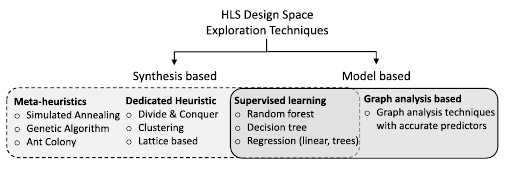
\includegraphics[width=1.0\textwidth]{Figures/HLS-taxonomy}
        \caption[Taxonomy for HLS based DSE approaches]{Taxonomy for HLS based DSE approaches, as proposed by Schafer \etal{} \cite{schafer_high-level_2020}}
        \label{ch.state:sec.strategies:fig.taxonomy}
    \end{figure}

    On the other hand, Barone \etal{} \cite{barone_multi-objective_2021} expose a substantial literature for \myAc{AxC}-based exploration, showing that specific domains have their own optimization problems, and claim that we need generic \myAc{DSE} framework to address those specificities.

    This section will thus expose a set of exploration initiatives based on introduced taxonomy from Schafer \etal{} \cite{schafer_high-level_2020} (Fig. \ref{ch.state:sec.strategies:fig.taxonomy}), and provide some insights about usage and limitations of considered approaches.

    \subsection{Meta Heuristics}
    \label{ch.state:sec.strategies:ssec.meta}
        A first class of exploration algorithms is based on meta heuristics, which are problem-independent heuristics that can be used to efficiently solve \myLongAcs{MOP}{Multi-objective Optimization Problem}.

        To begin with, \myLongAcs{GA}{Genetic Algorithm} have been used to perform \myAc{MOP} solving in an efficient way \cite{manuel_model-based_2020}.
        \myAc{GA} are evolutionary algorithms that relies on performing biologically inspired operations to evolve population toward better solutions, by model variations of implementation as potential mutations in a population of architecture.
        Dovado \cite{paletti_dovado_2021} exploit a {\bf Non-Dominated Genetic Algorithm} from \cite{shokri_algorithm_2013} to solve the \myAc{DSE} optimization problem, while Barone \etal{} \cite{barone_multi-objective_2021} provide an evolutionary search engine Bellerophon in their \eidea{} automatic exploration framework.
        This framework itself is an amelioration of $\mathbb{I}$DE$\mathbb{A}$ framework \cite{barbareschi_automatic_2016}, which was using a branch-and-bound approach to solve this optimization problem.

        We can also consider stochastic processes such as {\bf Bayesian optimization} for \myAc{MOP} solving, which can be used to optimize costly (\ie long to estimate) functions in an efficient fashion.
        To do so, multi-variate spaces are modelled using {\bf Gaussian processes} \cite{lo_model-based_2016}\cite{lo_multi-fidelity_2018}, and space exploration is then performed without having to exhaustively explore the whole space.
        This is the approach used by {\bf BOOM-Explorer} to efficiently propose a performant implementation of the \myAc{BOOM} core \cite{bai_boom-explorer_2021}: {\bf Gaussian processes} are used for initial set characterization (along with machine learning techniques), and {\bf Bayesian optimization} is then used for Pareto optimization of considered design space.

        Other meta heuristics for optimization have been exposed by Schafer \etal{} \cite{schafer_high-level_2020}, where biological and natural behaviours are used as model for optimization process, as it is the case with simulated annealing, for example.
        Simulated annealing is a Monte Carlo based method aiming to model the process of metal annealing, consisting in heating and cooling the metal in order to achieve a better stability.
        It can be used to approximate a global optimum for an optimization problem, by allowing to avoid local optima which could be found by simpler strategies, and was used to solve \myAc{DSE} problem by various initiatives, including Witschen \etal{} \cite{witschen_circa_2019}.

        As meta heuristic usage for \myAc{MOP} solving is a very wide research domain, we will not list every initiative to provide efficient manners of solving such problem.
        However, one should know that many algorithms can be used, and should consider them when building a \myAc{DSE} framework.        

    \subsection{Dedicated Heuristics}
    \label{ch.state:sec.strategies:ssec.dedicated}
        While meta-heuristics are problem-independent heuristics for optimization, dedicated heuristics are designed for specific problem solving.
        As \myAc{DSE} problem has been considered for decades now, many initiatives have proposed dedicated algorithms to perform efficient exploration, instead of trying to apply generic heuristics from other optimization domains.

        While Prost-Boucle \etal{} \cite{prost-boucle_fast_2014} propose a greedy approach to synthesize C algorithms under constraints (selecting and applying transforms in a sequential way to find Pareto optima), other approaches focus on quick estimation methodologies to perform exhaustive search of the space \cite{zhong_design_2017}\cite{bannwart_perina_fast_2021}.
        Other approaches uses the structure of design space itself to perform more efficient optimizations: for example, {\bf random sampling} of the space can be used, either to easily find Pareto optimum designs through neighbourhood exploration \cite{ye_scalehls_2021}, or to identify {\bf regions of interests} before performing sub region exploration through other processes such as search tree algorithms \cite{awais_ldax_2021}.
        In order to provide efficient exploration of the space, one can also consider iterative processes in a greedy approach --- \eg iteratively selecting next directive to optimize in \myAc{HLS} based processes \cite{siracusa_comprehensive_2021}, or using gradient based algorithms to find local optimum \cite{witschen_circa_2019}.

\clearpage
        Moreover, dedicated heuristics can also be defined for application specific explorations, with a rising needs for \myLongAc{CNN}{Convolutional Neural Network} implementation exploration \cite{motamedi_design_2016}\cite{park_roofline-model-based_2020}.
        This exhibits the specificities a domain can bring to the exploration problem, as well as the need for users to define specific explorations strategies for their use cases.

        More complex initiatives leverage multi-fidelity estimation: Dong Liu \etal{} \cite{dong_liu_efficient_2016} perform \myAc{HLS} based estimation of the whole space, then perform pruning before syntheses, using {\bf Rival Penalized Competitive Learning} to efficiently synthesize remaining implementations.
        In this way, they expose a need for a way to explicitly specify sequential exploration strategies to build complex strategy, while leveraging supervised learning methods to achieve efficient exploration.

    \subsection{Supervised Learning}
    \label{ch.state:sec.strategies:ssec.ml}
        As defined in exploration taxonomy from Figure \ref{ch.state:sec.strategies:fig.taxonomy}, both meta-heuristics and dedicated heuristics are synthesis based processes, meaning that they only consider synthesis (or other estimators) results to guide exploration.

        On the other hand, model based initiatives have been proposed in order to reduce the number of estimation processes to be run in an exploration process, thus accelerating the global flow.
        Supervised learning methods have thus emerged, leveraging synthesis generated knowledge to feed learning methods to be exploited later in the flow.

        Different uses of supervised learning have been proposed, from leveraging knowledge from prior explorations to speed-up the current one \cite{ferretti_leveraging_2020}, to fast simulated annealing using a decision tree \cite{mahapatra_machine-learning_2014}.
        
        Geng \etal{} \cite{geng_high-speed_2021} use {\bf Graph Neural Processing} to explore adder implementation, while Nardi \etal{} \cite{nardi_practical_2019} also leverage prior knowledge in {\bf Spatial} before using active learning under unknown feasibility constraints to provide Pareto approximation in their \myAc{DSE} engine.
        Liu \etal{} \cite{liu_learning-based_2013} study the usability of {\bf Random-Forest} algorithm for \myAc{HLS} based \myAc{DSE}, providing a comprehensive study on eight different learning models.
        Moreover, Meng \etal{} \cite{meng_adaptive_2016} provide an interesting approach to re-think machine learning usage for \myAc{DSE}, by using such methods to prune the design space before running end-to-end exploration using synthesis processes.

        Finally, {\bf BOOM-Explorer} \cite{bai_boom-explorer_2021} uses Gaussian process along with active learning and deep kernel learning functions for both initial set generation and design space characterization before employing Bayesian optimisation for exploration, showing that multiple approaches can be mixed to generate efficient exploration strategies.

    \subsection{Graph-Based Algorithms}
    \label{ch.state:sec.strategies:ssec.graph}
        The last class of \myAc{DSE} strategies in the considered taxonomy is purely based on modelling the whole synthesis flow instead of performing costly syntheses.

        Such initiatives include {\bf Lin-analyzer} \cite{zhong_lin-analyzer_2016}, which uses profiling to build a {\bf Dynamic Data Dependence Graph} (DDDG) model, {\bf COMBA} \cite{zhao_comba_2017}\cite{zhao_performance_2020}, a model based exploration framework for \myAc{HLS}, and {\bf FlexCL} \cite{wang_flexcl_2017}.
    
        This approach does expose the needs for expressivity for users to be able to build purely analytic models for exploration in their \myAc{DSE} framework.

    \subsection{Discussion on the Exploration Needs}
        A plethora of different approaches have been proposed in more or less recent initiatives in order to improve \myAc{DSE} processes, and various heuristics and algorithms should be considered by users aiming at implementing efficient exploration flows.

        Among those initiatives, some leverage multiple approaches by combining them for efficient exploration \cite{dong_liu_efficient_2016}\cite{bai_boom-explorer_2021}, displaying a need for flexibility in the process of building an exploration strategy ---  the designers should be able to define and guide their exploration based on both their applicative and technological expertises.

        In order to provide developers with such flexibility, a library of modular exploration passes should be proposed for efficient strategy building, allowing users to sequentially compose basic strategies to define more complex \myAc{DSE} operations in a given design space --- \eg leveraging quick estimation through learning methods for efficient pruning before running syntheses for more accurate results \cite{meng_adaptive_2016}.

\clearpage
\section{Synthesis on the Existing Approaches}
\label{ch.state:sec.synthesis}
    \subsubsection{Analysis of the literature}   
        In this chapter, we have provided an analysis of the existing \myLongAc{DSE}{Design Space Exploration} strategies in the literature, focussing on three main aspects --- the design space exposition, the metrics to be considered for both evaluation and comparison of different architectures, and the exploration strategies to be used to efficiently browse through a design space.

        We have identified some initiatives that could be considered to provide performant exploration frameworks, including wide research domains such as \myLongAc{HLS}{High Level Synthesis} and \myLongAcs{DSL}{Domain Specific Language}, and more recent approaches such as the \myLongAc{HCL}{Hardware Construction Language} paradigm.
        Among them, we put a particular focus on building flexible frameworks for strategy definition, such as the \myLongAc{AxC}{Approximate Computing} specific \eidea{} \cite{barone_multi-objective_2021}, which aims at proposing a generic exploration framework that allows its users to define application and target-independent strategies in an extensible fashion.

        In addition to this, we consider various taxonomies of exploration strategies, and among them the one proposed by Shathanaa \etal{} \cite{sa_design_2018}, where three strategy approaches are considered --- namely hierarchical approach, iterative approach, and sequential approach.
        We hereby identify an opportunity to leverage the composition of basic exploration strategies in a functional fashion, in order to provide the users with sequential approaches in their exploration framework.
    
    \subsubsection{Considered approach and planned contributions}
        Based on this analysis of the \myAc{DSE} research field, we plan to build an efficient exploration tool to ease the life of the hardware developers.
        More specifically, we examine providing a generic \myLongAc{FPGA}{Field-Programmable Gate Array} based exploration framework which would allow users to expose and control:
        \begin{itemize}
            \setlength\itemsep{-0.2cm}
            \item their own target and applicative domains
            \item their own design spaces
            \item their own metrics and estimation methodologies
            \item their own exploration strategies
        \end{itemize}
    
\clearpage
        To do so, the first step is hence to define how the design spaces are to be exposed in the framework.
        While we considered the usage of both \myAc{HLS} and \myAc{DSL}-based techniques for exposing explorable design spaces in this analysis, one can remark that such approaches have been widely explored in the past decades, resulting in the creation of multiple, industrially used frameworks.
        However, such tools are mainly based on the usage of architectural directives in the code to guide the exploration, and do not allow to finely control the generated accelerators as every choice that are not manually tuned by the developers are produced by automatic inference tools.
        On the other hand, some recent initiatives considered using \myLongAc{RTL}{Register-Transfer Level} languages to build generic exploration frameworks such as the one we are discussing here \cite{paletti_dovado_2021}.
        Nevertheless, they are based on standard \myLongAcs{HDL}{Hardware Description Language}, which are difficult to use and apprehend, and do not benefit from emerging paradigms to increase the productivity of the designers.
        To cope with those limitations, we hence consider using an \myAc{HCL} and its associated \myLongAc{HCF}{Hardware Construction Framework} to provide users with high level features for hardware development, while enabling to efficiently expose expertise-based design spaces.

        % As for the two other concerns --- namely the definition of the metrics of interests (as well as the corresponding estimation methodologies) and the description of the exploration strategies --- we consider implementing commonly used methodologies and algorithms as a {\it proof of concept}.
        As for the definition of the metrics of interest, as well as the corresponding estimation methodologies, we consider implementing the most commonly used methodologies as a {\it proof of concept}.
        However, some other approaches among the ones that have been presented in this chapter could be applied to build meaningful ways to evaluate and compare architectures, in order to provide users with both modularity and flexibility in their design processes.
        Indeed, some other initiatives cannot be applied in this context --- \eg considering an \myAc{HCL} as the entry point of the exploration flows is not compatible with the estimation methodologies that rely on an algorithmic description of the circuits behaviours, as it is the case for most of the \myAc{HLS}-based latency and resource estimators.

        Finally, when it comes to the exploration strategies, most of the considered algorithms can be applied for \myAc{DSE} regardless of the exposition of the design space --- except for graph-based algorithms, which also require an algorithmic description to be used.
        In this context, and even if we only consider implementing basic strategies in a first time, one could consider each of those approaches to build a configurable library of exploration algorithms, hence providing the users with a generic and modular tool.

\clearpage
    \subsubsection{Identified limitations}

        After defining the scope of this work, as well as the planned contributions, we identify some limitations about the proposed approach.

        First of all, it will require its users to explicitly expose the design space, thus requiring expertise about both the algorithm and the target board.
        It is quite different from the \myAc{HLS} approach, for example, where the design space is essentially defined by the transformations performed by the \myAc{HLS} tool to generate the accelerators, that are quite transparent for the developers.

        Moreover, our approach will require the users not only to define the design space to be explored (by exposing the generation parameters as architectural knobs), but also to describe the different generators of accelerators in a \myAc{RTL}-based language, which also requires a lot of time and expertise.

        Last but not least, we will only consider sequential exploration strategies in this work, which could be a limitation for the algorithms relying on parallel and interacting steps for instance.
        
        However, we propose to explore the opportunity of building a fully configurable exploration framework, that would leverage the features of recent \myAcs{HCF} to facilitate the life of hardware developers.


%%%%%%%%%%%%%%%%%%%%%%%%%%%%%%%%%%%%%%%%%%%%%%%%%%%%%%%%%%%%%%%%%%%%%%%%%%%%%%%%
%%%%%%%%%%%%%%%%%%%%%%%%%%%%%%%%%%%%%%%%%%%%%%%%%%%%%%%%%%%%%%%%%%%%%%%%%%%%%%%%

\cleardoublepage
%-------------------------------------------------------------------------------
\chapter{Building and Integrating Estimators}
\labelchapter{ch.estimators}
%-------------------------------------------------------------------------------

%%%%%%%%%%%%%%%%%%%%%%%%%%%%%%%%%%%%%%%%%%%%%%%%%%%%%%%%%%%%%%%%%%%%%%%%%%%%%%%%
%%%%%%%%%%%%%%%%%%%%%%%%%%%%%%%%%%%%%%%%%%%%%%%%%%%%%%%%%%%%%%%%%%%%%%%%%%%%%%%%

\lettrine[lines=2]{T}{his} chapter discusses the definition of metrics used in hardware development processes, as well as their integration in a \myLongAc{HCF}{Hardware Construction Framework}.
We then consider different types of metrics to be used for hardware development, as well as various ways to estimate them, and finally expose a generic \myLongAc{API}{Application Programming Interface} for users to build their own estimation methodologies.

\vspace*{\fill}
\minitoc 
\mtcskip 

\newpage
%%%%%%%%%%%%%%%%%%%%%%%%%%%%%%%%%%%%%%%%%%%%%%%%%%%%%%%%%%%%%%%%%%%%%%%%%%%%%%%%

\section{Importance of Qualitative Estimations}
\label{ch.estimators:sec.estimators}
    In order to build efficient hardware designs under various constraints --- such as resource usage, power consumption or exploitable throughput --- hardware developers require quantitative estimations to make the best decision possible.
    However, design processes remain time-consuming tasks, and standard design methodologies rely on heavy computations --- \eg logic synthesis --- to obtain exploitable feedback, resulting in long turnaround times.
    In this section, we will consider different metrics and the quality of estimators to retrieve them, then discuss the importance of qualitative estimators for hardware design, and more specifically for \myLongAc{DSE}{Design Space Exploration}.

    \subsection{Quality of the Estimators}
    \label{ch.estimators:sec.estimators:ssec.quality}
        Various metrics can be used to define the quality of a hardware implementation, depending on the target circuit environment and the objectives of the developed accelerators.
        Among the most used metrics are resource usage, operating frequency, circuit latency or power consumption.
        However, they need to be adapted to the running environment of the design --- \eg resource usage can be defined as the area of silicon used when building \myLongAcs{ASIC}{Application-Specific Integrated Circuit}, but is most difficult to define for \myLongAc{FPGA}{Field-Programmable Gate Array} design, as multiple resources have to be considered due to the inherent heterogeneity of the boards (Fig. \ref{ch.problem:sec.hardware:ssec.fpga:sssec.fpga:fig.clb}).

        The quality of estimations needs to be considered to build efficient designs and exploration flows, as using poor estimators will more than probably result in a poor decision by the designer or by the exploration framework.
        However, we first need to define what is the quality of an estimator for a given metric, in order to quantify and compare multiple estimation techniques.
        Quality of an estimator can only be defined with respect to a reference value, \ie the expected value for the metric being estimated.
        In the rest of this work, we will consider {\bf synthesis results} as the reference value for both resource and frequency metrics, and consider estimators \myLongAc{QoR}{Quality of Results}\footnote{In the context of this thesis, both \myLongAc{QoR}{Quality of Results} and \myLongAc{QoS}{Quality of Service} notions will be used. Please refer to the glossary for disambiguation purposes.} with respect to vendor specific tools such as \tn{vivado} or \tn{Quartus}.

        In order to quantify quality estimators, we consider three aspects of an estimation methodology: {\bf accuracy}, {\bf faithfulness} and {\bf speed}.
        {\bf Accuracy} is defined as the proximity of the estimations to the expected values, while {\bf faithfulness} is defined using the standard deviation of the estimations --- \ie variation of estimators accuracy on different implementations.\footnote{Estimators \myAc{QoR} should thus consider both notions.}
        As a result, estimators can have high faithfulness but low accuracy --- \eg always estimating twice as many resources allows to easily compare different architectures, but can result in wrong design decisions as estimations are far from real values.
        Finally, {\bf speed} is defined with respect to the time needed to perform estimation.

        In this context, estimation methodologies offer different trade-offs between speed, accuracy and faithfulness, and estimator usage depends on the design goal.
        For example, to validate that a circuit is suitable for a given constraint set, one may consider slow but accurate estimations.
        Conversely, performing \myAc{DSE} requires fast and faithful estimators, but accuracy is not a main concern as the focus is put on comparing hardware implementations.

        We built Table \ref{ch.estimators:sec.estimators:ssec.quality:table.comparison} using our expertise and the literature introduced in Chapter \ref{ch.state}.
        It presents different estimation methodologies, as well as the corresponding quality metrics, showing different trade-offs depending on the usage.
        Standard \myLongAc{RTL}{Register-Transfer Level} methodologies are used as a baseline (Fig. \ref{ch.problem:sec.hardware:ssec.paradigms:fig.rtl}), since they are used to generate the reference values.
        Various works have explored rapid \myAc{RTL}-based estimations of both resource usage and operating frequency.
        However, critical paths are almost impossible to accurately estimate without running whole standard processes, therefore, \myAc{RTL}-based methodologies are not appropriate for such estimations.
        To cope with this challenge, \myLongAc{HLS}{High Level Synthesis} methodologies rely on fast resource estimations to allow quick exploration of the design space, but most tools use latency estimation and automatic scheduling rather than frequency estimation, in order to build accurate and controllable timing estimations.
        As for Spatial, it provides quick, reasonably faithful and accurate estimators, but the framework relies on a \myLongAc{DSL}{Domain Specific Language}, and is hence not adaptable to every possible use case.

        As a result, different metrics and estimation methodologies are to be considered for hardware development, depending on use case specificities --- this aspect is known as {\bf multi-fidelity metrics} usage and was already considered in the context of \myAc{HLS} exploration \cite{lo_multi-fidelity_2018}.

    \begin{table}[ht!]
        \centering
        \begin{adjustbox}{width=1.0\columnwidth,center}
            \begin{tabular}{c|ccccc}
                {\bf Entry level} & {\bf Metric} & {\bf Tools} & {\bf Accuracy} & {\bf Faithfulness} & {\bf Speed}\\
                \hline
                \multirow{2}*{RTL} & \ccg Resource, & \ccg Synthesis & \ccg & \ccg & \ccg \\
                ~ & \ccg frequency & \ccg (\tn{vivado}, \tn{Quartus}) & \ccg \multirow{-2}*{High} & \ccg \multirow{-2}*{High} & \ccg \multirow{-2}*{Slow}\\
                \multirow{2}*{RTL} & \multirow{2}*{Resource} & RTL estimation & \multirow{2}*{Low} & \multirow{2}*{Medium} & \multirow{2}*{Fast}\\
                ~ & ~ & \cite{schumacher_fast_2008}\cite{deng_accurate_2008} & ~ & ~ & ~\\
                \multirow{2}*{HLS} & \ccg Resource, & \ccg HLS tools & \ccg & \ccg & \ccg \\
                ~ & \ccg latency & \ccg \cite{canis2011legup}\cite{xilinx_vivado_2021} & \ccg \multirow{-2}*{Low} & \ccg \multirow{-2}*{Medium} & \ccg \multirow{-2}*{Fast}\\
                \multirow{2}*{DSL} & Resource, & \multirow{2}*{Spatial \cite{nardi_practical_2019}} & \multirow{2}*{Medium} & \multirow{2}*{Medium} & \multirow{2}*{Fast}\\
                ~ & frequency & ~ & ~ & ~ & ~\\
                \hline
            \end{tabular}
        \end{adjustbox}
        \caption[Estimation quality and abstraction level]{Comparison of different estimators depending on abstraction level}
        \label{ch.estimators:sec.estimators:ssec.quality:table.comparison}
    \end{table}

    \subsection{Feedback Usage for Hardware Development}
    \label{ch.estimators:sec.estimators:ssec.feedback}
        After defining qualitative concerns about metric estimators, we consider the different uses of metric estimation for hardware development processes.
        
        In standard \myAc{RTL} methodologies, iterating over produced designs is a time-consuming task as obtaining feedback about the developed circuit quality can take up to days of complex tool usage such as synthesis or place and route.
        To increase productivity, quick estimators can be used to swiftly provide feedback to developers, guiding them toward acceptable solutions while reducing the time spent in heavy computations --- however, significant time is still needed at the end of the process to validate that a design actually fits on the target board.
        
        Moreover, qualitative estimators are primordial for efficient \myAc{DSE}, as exploration speed is a main challenge for such methodologies --- actually, two levers can be considered to speed up exploration processes, namely exploration strategies and estimation methodologies.
        As exploration strategies will be considered in Chapter \ref{ch.dse}, this chapter will be dedicated to discussing the impact of estimation methodologies on \myAc{DSE} processes.

        As such processes are based on architecture comparisons in order to determine the impact of implementation options on resulting designs, one of the main challenges is related to how architectures should be compared.
        Thereupon, quick but faithful estimators need to be considered in such processes to perform meaningful comparisons in a reduced amount of time. 

%%%%%%%%%%%%%%%%%%%%%%%%%%%%%%%%%%%%%%%%%%%%%%%%%%%%%%%%%%%%%%%%%%%%%%%%%%%%%%%%

\section{Resource and Timing Estimations}
\label{ch.estimators:sec.resource-timing}

    Resource usage and timing concerns (\eg operating frequency, circuit latency) are among the principal considerations when it comes to \myAc{FPGA} development, as target specific constraints are to be respected for a design to pass the validation process.
    However, as stated in Section \ref{ch.estimators:sec.estimators}, classical flows used to produce such metrics are time consuming, resulting in long iterations over generated designs to find a suitable solution.

    This section hence considers building fast resource and timing estimators based on the \myLongAc{HCL}{Hardware Construction Language} paradigm to speed up its usage --- more specifically, we consider a \chisel{} based implementation.
    The aim is not to build state of the art estimators with particular focus on a good accuracy, but rather to integrate {\it proof of concept} estimators in an \myLongAc{HCF}{Hardware Construction Framework} and consider their usage as a way to increase hardware developer productivity.

    In order to do so, we chose to implement a resource estimation methodology similar to the one introduced by Schumacher \etal{} \cite{schumacher_fast_2008}, based on operator characterization and an \myLongAc{API}{Application Programming Interface} allowing users to model compilation steps that the synthesis tool is expected to take in order to provide realistic estimations.

    \subsection{Intermediate Representation Usage}
    \label{ch.estimators:sec.resource-timing:ssec.ir}

        Using \chisel{} as an entry point for a hardware development flow, one still requires a \myAc{HCF} to perform circuit elaboration, optimizations and backend emission, allowing the generated design to be fed to any \myAc{RTL} based toolchain.
        As an \myAc{HCF} requires an \myLongAc{IR}{Intermediate Representation} to operate on --- as does any compiler --- \myLongAc{FIRRTL}{Flexible Intermediate Representation for RTL} \cite{li_2016_specification}\cite{izraelevitz_2017_reusability} was introduced along \chisel{}.
        It was primarily built as an initiative to use \myAcs{HCL} for parametrized hardware library building, abstracting technology specific knowledge from the \myAc{HCF} frontend and relying on further transforms and backend to transform target-independent \myAc{RTL} to technology specific \myAc{RTL} --- allowing, for example, to use the same \chisel{} for both \myAc{ASIC} and \myAc{FPGA} targets.
        As a matter of fact, adapting software compilers structure --- \ie separating entry language (frontend), \myAc{IR} transforms and code generation (backend) --- enables to reuse \myAc{HCL} code, instead of using {\it ad-hoc} scripts to replace specific structures in the entry code to target a particular technology, as is usually done in standard development processes.
        Such target specific transforms can now be enabled by operating directly on the \myAc{IR}, and modifying the target technology becomes as simple as changing the transforms and configuration used for generation.
        Moreover, as both \chisel{} and \firrtl{} are based on \scala, high level programming features can be used for both hardware generator description and transform definition, enhancing developers expressivity for hardware description.

        Thereupon, to integrate estimators in an \myAc{HCF}, one must consider defining \myAc{IR} transforms as a way to operate on a given circuit and provide metric estimations in the process.

\clearpage
    \subsection{Basic Operator Characterization}
    \label{ch.estimators:sec.resource-timing:ssec.basic}

        Our first approach to build \firrtl{} based estimators is based on a naive approach of digital circuits, considering each operator individually on data paths, adding individual metrics to build global estimators.

        To begin with, we oppose costly \vs non costly operators --- based on our designer experience --- in Table \ref{ch.estimators:sec.resource-timing:ssec.basic:table.operator}, considering impact on both resource usage and data paths traversal time.

        \begin{table}[ht!]
            \centering
            \begin{adjustbox}{width=1.0\columnwidth,center}
                \begin{tabular}{c|ccc}
                    \multirow{2}*{{\bf Operator}} & \multirow{2}*{{\bf Description}} & \multirow{2}*{{\bf Impacting parameters}} & {\bf Considered}\\
                    ~ & ~ & ~ & {\bf for estimation}\\
                    \hline
                    {\tt ADD} & \ccg Adders & \ccg Operand widths & \ccg {\bf yes}\\
                    {\tt MULT} & Multipliers & Operand/result widths & {\bf yes}\\
                    \multirow{2}*{{\tt BINOP}} & \ccg Binary operations & \ccg ~ & \ccg ~\\
                    ~ & \ccg ({\tt OR}, {\tt AND}, {\tt NOT}, ...) & \multirow{-2}*{\ccg Operand widths} & \multirow{-2}*{\ccg {\bf yes}}\\
                    {\tt MUX} & Multiplexers & Operand/Condition widths & {\bf yes}\\
                    {\tt DSHIFT} & \ccg Dynamic shifts & \ccg Shift/result widths & \ccg {\bf yes}\\
                    {\tt REGISTER} & Registers & Element width & {\bf yes}\\
                    {\tt MEMORY} & \ccg Memory primitives & \ccg Memory width and depth & \ccg {\bf yes}\\
                    {\tt SSHIFT} & Static shifts & Input width & no\\
                    {\tt SELECT} & \ccg Bit selection among words & \ccg Result width & \ccg no\\
                    {\tt PAD} & Word padding & Result width & no\\
                    {\tt CAT} & \ccg Word concatenation & \ccg Result width & \ccg no\\
                    {\tt CONVERT} & Type conversion & Operand type and width & no\\
                    {\tt IO} & \ccg Input/output & \ccg Source/dest width & \ccg no\\
                    {\tt CONST} & Constant definition & Constant value & no\\
                    {\tt CONNECT} & \ccg Signal connection & \ccg Source/dest widths & \ccg no\\
                \end{tabular}
            \end{adjustbox}
            \caption[Operator impacts on estimations]{Operator impacts on both timing and resource usage estimations}
            \label{ch.estimators:sec.resource-timing:ssec.basic:table.operator}
        \end{table}

        To define non costly operators, we consider operations that are mostly reduced to rewiring of signals, as such action does not require particular resource usage but routing resources, and as wire traversal is considered non significant in this approach.% --- even if, for \myAc{FPGA} designs, Xu \etal{} \cite{xu_area_1996} up to 60\% of the critical path delay comes from routing.

        After identifying operators to consider for estimation, we use a pre-characterization based approach.
        To do so, we use vendor specific tools --- such as the \vivado{} synthesis tool for Xilinx \myAcs{FPGA} --- to generate {\bf reference values} for both resource usage and operator traversal time.
        Operators are characterized for a given set of different operand bit widths --- for example, adders are characterized with operands on 1, 2, 4, ..., 256 bits --- storing all the results in a {\bf library file} (using the \myAc{JSON} format).\footnote{Different operand widths are not considered in this process to enable single parameter characterization, thus only maximum operand bit width is considered for estimation in this naive approach.}
        Once this is done, we can use this characterized library to estimate both resource usage and timing of a given operator, using maximum operand bit width in the \firrtl{} representation as a parameter for estimation.
        The estimation process is then based on a simple statistical model: we retrieve the two nearest results --- \ie nearest maximum operand bit widths --- for an operator from the library, and estimate both resource usage and data path cost using linear regression between those two results, for each considered metrics.

        A first distinction is then to be made between resource and timing estimation: while we can estimate global resource usage by adding each individual operator estimation --- for each metric considered (\eg \myAcs{LUT}, \myAcs{FF}, \myAcs{DSP} and \myAcs{BRAM}) --- we need further circuit analysis to provide interesting timing estimations.

        \underline{Remark:} characterization is not mandatory for {\tt REGISTER} resource estimation as technological mapping is quite straightforward --- a n bit register will only use n \myAcs{FF}. 
        As for {\tt MEMORY} primitive estimations, both width and depth should be considered for estimation, and characterization is not needed either for the same reason.
        We thus use an {\it ad-hoc} computation of memory resource, based on a simple estimation of the total amount of bit in the {\tt MEMORY} primitive ($depth \times width$).

    \subsection{Data Path Building}
    \label{ch.estimators:sec.resource-timing:ssec.path}

        Timing considerations for hardware design are mainly based on the notion of {\bf critical path}.
        Critical path is defined as the longest path in the circuit --- each path corresponding to a sequence of wires and transistors from a starting point to an ending point, the longest being the one where the total traversal time is the greatest.
        In the context of synchronous designs, both starting and ending points are mostly defined as memory primitives, being either registers (\myAcs{FF}) or more complex memory components (\eg \myAcs{BRAM}).
        Circuit \myAcs{IO} are also to be considered for critical path definition, as they represent the interface with the external world, and may impact on the operating frequency.
        Maximal operating frequency is then defined as the inverse of the longest path traversal time, as operating at a higher frequency will result in some computation signals not being saved before new computations start.

        In order to provide a maximum operating frequency estimation based on \firrtl{}, we thus have to estimate traversal time of each possible path in the circuit, compare them, and expose the longest one(s) to users. 
        We consider three different cases in the process: register to register paths, \myAc{IO} to register paths, and register to \myAc{IO} paths. 
        It is important to note that the \firrtl{} representation uses a hierarchical approach for describing a circuit --- like do standard \myAcs{HDL} such as \verilog{} or \vhdl{} --- which is used to describe a complex circuit as a composition of simpler parts, the {\bf modules}.
        The main circuit of a design process is denoted as being the {\bf top level module}, and corresponds to the main \chisel{} class being compiled.
        One of the main challenges is hence to build every possible path, including {\bf cross-module} ones --- \ie paths originating in a module and terminating in another one --- which requires multiple passes over the circuit representation.

        Once every possible path is built, we can finally use individual operator traversal time estimations built in Section \ref{ch.estimators:sec.resource-timing:ssec.basic}.
        We consider a basic, addition based approach, where every estimation in a given path are added to estimate its total traversal time.
        We then compare each path traversal time, and provide users with feedback on timing concerns.

        \begin{figure}[h!]
            \centering
            \begin{subfigure}{1.0\textwidth}
                \centering
                \begin{adjustbox}{width=1.0\columnwidth,center}
                    \begin{tabular}{c|c|cccc|c}
                        {\bf Operator} & {\bf Bit width} & {\bf LUT} & {\bf FF} & {\bf DSP} & {\bf BRAM} & {\bf Path (ns)}\\
                        \hline
                        \multirow{3}*{{\tt ADD}} & \ccg 16 & \ccg 16 & \ccg 0 & \ccg 0 & \ccg 0 & \ccg 1.296\\
                        ~ & \ccg 32 & \ccg 32 & \ccg 0 & \ccg 0 & \ccg 0 & \ccg 1.512\\
                        ~ & \ccg 64 & \ccg 64 & \ccg 0 & \ccg 0 & \ccg 0 & \ccg 1.944\\
                        \multirow{3}*{{\tt MULT}} & 16 & 0 & 0 & 1 & 0 & 1.228\\
                        ~ & 32 & 0 & 0 & 4 & 0 & 4.176\\
                        ~ & 64 & 0 & 0 & 16 & 0 & 5.439\\
                        \multirow{3}*{{\tt REGISTER}} & \ccg 16 & \ccg 0 & \ccg 16 & \ccg 0 & \ccg 0 & \ccg 0.695\\
                        ~ & \ccg 32 & \ccg 0 & \ccg 32 & \ccg 0 & \ccg 0 & \ccg 0.695\\
                        ~ & \ccg 64 & \ccg 0 & \ccg 64 & \ccg 0 & \ccg 0 & \ccg 0.695\\
                    \end{tabular}
                \end{adjustbox}
                \caption{Characterized operator library for estimation (\Xilinx{} \VC{} board)}
                \label{ch.estimators:sec.resource-timing:ssec.basic:fig.estimation:sfig.lib}
                \vspace{1em}
            \end{subfigure}
            \begin{subfigure}{1.0\textwidth}
                \centering
                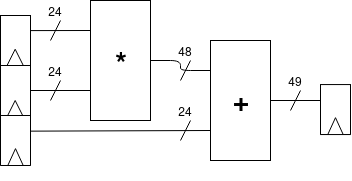
\includegraphics[width=0.65\textwidth]{Figures/Estimation-noMacro.png}
                \caption{Example of a simple circuit to estimate}
                \label{ch.estimators:sec.resource-timing:ssec.basic:fig.estimation:sfig.mac}
                \vspace{1em}
            \end{subfigure}
            \begin{subfigure}{1.0\textwidth}
                \centering
                \begin{adjustbox}{width=1.0\columnwidth,center}
                    \begin{tabular}{c|cc|cccc|c}
                        {\bf Operator} & {\bf \#} & {\bf Bit width} & {\bf LUT} & {\bf FF} & {\bf DSP} & {\bf BRAM} & {\bf Path (ns)}\\
                        \hline
                        {\tt ADD} & \ccg 1 & \ccg 32 & \ccg 32 & \ccg 0 & \ccg 0 & \ccg 0 & \ccg 1.512\\
                        {\tt MULT} & 1 & 24 & 0 & 0 & 3 & 0 & 2.702\\
                        {\tt REGISTER} & \ccg 3 & \ccg 24 & \ccg 0 & \ccg 24 & \ccg 0 & \ccg 0 & \ccg 0.695\\
                        {\tt REGISTER} & 1 & 49 & 0 & 49 & 0 & 0 & 0.695\\
                        \hline
                        {\bf Circuit} & ~ & ~ & 32 & 121 & 3 & 0 & 4.909 
                    \end{tabular}
                \end{adjustbox}
                \caption{Simple estimation of resource usage and critical path for a simple circuit (Fig. \ref{ch.estimators:sec.resource-timing:ssec.basic:fig.estimation:sfig.mac})}
                \label{ch.estimators:sec.resource-timing:ssec.basic:fig.estimation:sfig.results}
            \end{subfigure}
            \caption[Basic estimation methodology]{Basic estimation methodology based on individual characterization}
            \label{ch.estimators:sec.resource-timing:ssec.basic:fig.estimation}
        \end{figure}

        Figure \ref{ch.estimators:sec.resource-timing:ssec.basic:fig.estimation} introduces an example of this estimation methodology usage on a simple circuit (Fig. \ref{ch.estimators:sec.resource-timing:ssec.basic:fig.estimation:sfig.mac}), when targeting a \Xilinx{} \VC{} board.
        Sub results in Table \ref{ch.estimators:sec.resource-timing:ssec.basic:fig.estimation:sfig.results} are computed using characterized values from Table \ref{ch.estimators:sec.resource-timing:ssec.basic:fig.estimation:sfig.lib} and simple linear regression --- \eg for {\tt MULT} operator estimation on 24 bits, each value is computed using the average of values on both 16 and 32 bits.
        Then, for resource estimation, each individual estimation is added, while for critical path estimation, all paths are compared.
        
        In this case, critical path goes from a 24 bits register to the 49 bits register through both {\tt MULT} and {\tt ADD} operations, resulting in a total traversal time of $0.695 + 1.512 + 2.702 = 4.909$ ns\footnote{The {\tt REGISTER} traversal time is considered only once in the critical path.} --- corresponding to a maximum operating frequency of 204 MHz.


    \subsection{Limitations of the Approach}
    \label{ch.estimators:sec.resouce-timing:ssec.limitations}

        While this first approach for both resource and timing estimation is simple to apprehend, it presents some heavy limitations.

        First of all, the operators are estimated using only the maximum operand bit width as parameter.
        Nonetheless, some operators might require some additional parameters, as shown in Table \ref{ch.estimators:sec.resource-timing:ssec.basic:table.operator} --- such as {\tt MEMORY} primitives, {\tt MUXes} or {\tt DSHIFTs}.

        Moreover, the heterogeneous structure inherent to \myAcs{FPGA} led developers to consider specific design patterns, in order to take advantage of available resources on a given target.
        For example, \myLongAc{MAC}{Multiply and Accumulate} operations are commonly used in domains such as signal or image processing, and can use \myAcs{DSP} --- if available --- to favourably replace \myAcs{LUT} and improve performance while reserving resources for other computations.
        Such usage cannot be expressed when considering operators as individual entities, and higher granularity should be enabled in the flow.

        Finally, data paths can heavily differ depending on many factors such as the operation, the operands or the target.
        For instance, adders are usually implemented using {\bf carry adders}, each result bit being generated in a sequential way --- the first bit only requiring a 2 bit logical operation, while the n bit require every results in $[\![0, n-1]\!]$ to compute the input carry.
        Let $t_n$ be the traversal time of a n bit adder.
        We consider chaining two n bit adders $a_0$ and $a_1$, with the output of $a_0$ being one of the operand of $a_1$.
        Our naive approach consider the total traversal time of the path as being $2 \times t_n = t_{2\times n}$, however computations in $a_1$ can begin after only $t_1$, as computing $a_1$ first bit only requires knowledge about the first bit of $a_0$ result.
        This means that most of the total traversal time of this path is actually absorbed in a pipeline fashion, with a total traversal time of $t_{n+1}$ instead of $t_{2\times n}$.

        All of these properties must be considered in order to build exploitable estimators --- \ie estimators that may help designers into taking advantageous decisions in the development process --- as not considering them might result in erroneous feedback.

    \subsection{Macro Block Replacement}
    \label{ch.estimators:sec.resource-timing:ssec.macro}

        \begin{figure}[h!]
            \centering
            \begin{subfigure}{1.0\textwidth}
                \begin{adjustbox}{width=1.0\columnwidth,center}
                    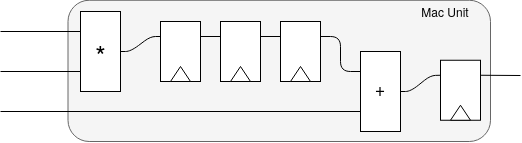
\includegraphics[width=1.0\textwidth]{Figures/MacroBlocks-Mac.png}
                \end{adjustbox}
                \caption{{\tt MAC} unit {\bf macro block} example for pattern $(R^3)(+^1)(R^1)$}
                \label{ch.estimators:sec.resource-timing:ssec.macro:fig.mac:sfig.pattern}
                \vspace{1em}
            \end{subfigure}
            \begin{subfigure}{1.0\textwidth}
                \begin{adjustbox}{width=1.0\columnwidth,center}
                    \begin{tabular}{c|c|cc}
                        {\bf Name} & {\bf Description} & {\bf Type} & {\bf Range}\\
                        \hline
                        \ccg {\it bit width} & \ccg maximum input bit width & \ccg generation & \ccg $[\![1, 256]\!]$\\
                        {\it outFactor} & useful output bit width & configuration & $[\![1, 2]\!]$\\
                        \ccg {\it mult register} & \ccg number of {\tt REGISTER} after {\tt MULT} & \ccg configuration & \ccg $[\![0, 3]\!]$\\
                        {\it add number} & number of {\tt ADD} in the {\tt MAC} pattern & configuration & $[\![0, 1]\!]$\\
                        \ccg {\it add register} & \ccg number of {\tt REGISTER} after {\tt ADD} & \ccg configuration & \ccg $[\![0, 1]\!]$
                    \end{tabular}
                \end{adjustbox}
                \caption{{\tt MAC} unit {\bf macro block} parameters w.r.t. \Xilinx{} \VC{} specifications}
                \label{ch.estimators:sec.resource-timing:ssec.macro:fig.mac:sfig.params}
            \end{subfigure}
            \caption[Multiply and accumulate macro block]{{\tt MAC} unit {\bf macro block}}
            \label{ch.estimators:sec.resource-timing:ssec.macro:fig.mac}
        \end{figure}
                
        \begin{figure}[h!]
            \centering
            \begin{subfigure}{0.85\textwidth}
                \begin{adjustbox}{width=0.5\columnwidth,center}
                    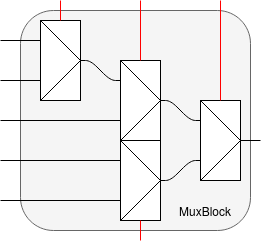
\includegraphics[width=1.0\textwidth]{Figures/MacroBlocks-MuxBlock.png}
                \end{adjustbox}
                \caption{{\tt MUXBLOCK} example with 5 inputs and 4 conditions}
                \label{ch.estimators:sec.resource-timing:ssec.macro:fig.mux:sfig.pattern}
                \vspace{1em}
            \end{subfigure}
            \begin{subfigure}{0.85\textwidth}
                \begin{adjustbox}{width=1.0\columnwidth,center}
                    \begin{tabular}{c|c|cc}
                        {\bf Name} & {\bf Description} & {\bf Type} & {\bf Range}\\
                        \hline
                        \ccg {\it bit width} & \ccg maximum input bit width & \ccg generation & \ccg $[\![1, 256]\!]$\\
                        {\it input number} & number of inputs & configuration & $2^{i, i \in [\![1, 8]\!]}$\\
                        \ccg {\it condition number} & \ccg number of conditions & \ccg configuration & \ccg $2^{i, i \in [\![0, 8]\!]}$\\
                    \end{tabular}
                \end{adjustbox}
                \caption{{\tt MUXBLOCK} parameters w.r.t. \Xilinx{} \VC{} specifications}
                \label{ch.estimators:sec.resource-timing:ssec.macro:fig.mux:sfig.params}
            \end{subfigure}
            \caption[Multiplexer macro block]{{\tt MUXBLOCK} {\bf macro block}}
            \label{ch.estimators:sec.resource-timing:ssec.macro:fig.mux}
        \end{figure}

        \begin{figure}[h!]
            \centering
            \begin{subfigure}{0.85\textwidth}
                \begin{adjustbox}{width=0.8\columnwidth,center}
                    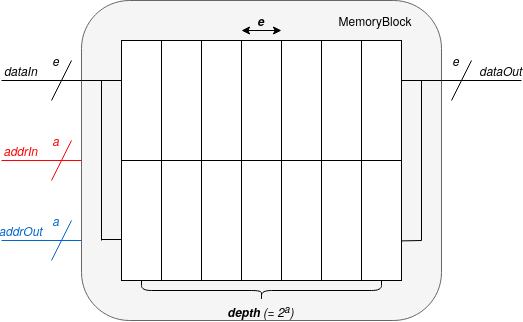
\includegraphics[width=1.0\textwidth]{Figures/MacroBlocks-MemoryBlock.png}
                \end{adjustbox}
                \caption{{\tt MEMORYBLOCK} schematic}
                \label{ch.estimators:sec.resource-timing:ssec.macro:fig.memory:sfig.pattern}
                \vspace{1em}
            \end{subfigure}
            \begin{subfigure}{0.85\textwidth}
                \begin{adjustbox}{width=1.0\columnwidth,center}
                    \begin{tabular}{c|c|cc}
                        {\bf Name} & {\bf Description} & {\bf Type} & {\bf Range}\\
                        \hline
                        \ccg {\it element width} & \ccg memory element bit width & \ccg generation & \ccg $[\![1, 1024$\\
                        {\it address number} & number of addresses & generation & $2^{i, i \in [\![1, 16]\!]}$\\
                        \ccg {\it register number} & \ccg number of register on address lines & \ccg configuration & \ccg $[\![0, 1]\!]$\\
                    \end{tabular}
                \end{adjustbox}
                \caption{{\tt MEMORYBLOCK} parameters w.r.t. \Xilinx{} \VC{} specifications}
                \label{ch.estimators:sec.resource-timing:ssec.macro:fig.memory:sfig.params}
            \end{subfigure}
            \caption[Memory macro block]{{\tt MEMORYBLOCK} {\bf macro block}}
            \label{ch.estimators:sec.resource-timing:ssec.macro:fig.memory}
        \end{figure}

        In order to improve this first approach, we now propose to consider more complex patterns for estimation, modelling steps that the synthesis tool is expected to take to pack operators \cite{schumacher_fast_2008}.
        To keep the method generic, we define two main steps for pattern recognition, replacement and estimation, and consider a user trying to find and replace $x$ different pattern $[\![p_0, ..., p_{x-1}]\!]$ in a \firrtl{} representation of a circuit.

        First of all, they need to define which pattern they are looking for, with respect to the \firrtl{} representation.
        To do so, we build a \myLongAc{DG}{Directed Graph} from a circuit \firrtl{} representation to operate on.
        We then developed a set of custom utility functions to scan the \myAc{DG}, recognize patterns and replace them by {\bf macro blocks} in the graph.
        We thus search and replace each pattern $p_{i, i \in [\![0, x-1]\!]}$ in the \myAc{DG} representation in a sequential fashion, therefore capturing complex computation patterns.
        At the end of the process, an updated \firrtl{} representation of the input circuit is produced in which all operators recognized as belonging to a particular {\bf macro block} are replaced by the corresponding {\bf macro block}.
        The \myAc{HCF} flow can then continue, and this representation can be fed into further \firrtl{} transforms --- \eg for estimation purposes.

        The second step is used to characterize the {\bf macro blocks} in a way similar to the one described in Section \ref{ch.estimators:sec.resource-timing:ssec.basic}.
        The user thus needs to provide a \chisel{} implementation generator for each pattern $p_{i, i \in [\![0, x-1]\!]}$, which is used to generate the {\bf reference values} for both resource usage and traversal time, using vendor tools such as \vivado{} syntheses.
        The generated values are then used to enhance the operator library with new parametrized {\bf macro blocks}.
        
        However, as stated in Section \ref{ch.estimators:sec.resource-timing:ssec.basic}, the first approach only considered single parameter estimation based on operator input bit width.
        To cope with such limitations, we consider two types of parameters to enhance the estimation process --- namely {\bf configuration parameters} and {\bf generation parameters}.
        The main difference between those two types is the value set width: {\bf configuration parameters} can be explored exhaustively for library building while {\bf generation parameters} would require too many runs and are thus only explored on a value subset for library building, before using linear regression for estimation as was done for bit widths in previous sections.
        Doing so enhances the library quality by adding a new entry for each possible configuration --- \ie each configuration in the cardinal product of {\bf configuration parameters} --- and each entry defines a regression based estimator for each considered metric (\myAc{LUT}, \myAc{FF}, \myAc{DSP}, \myAc{BRAM} and delay path), using {\bf generation parameters} as arguments of estimation functions.
        
        Three {\bf macro blocks} were considered to the enhanced basic operator library described in the first approach: \myLongAc{MAC}{Multiply and Accumulate} units, complex {\tt MUXBLOCK}s, and {\tt MEMORYBLOCK}s.
        Figure \ref{ch.estimators:sec.resource-timing:ssec.macro:fig.mac} introduces the {\tt MAC} unit macro blocks patterns and parameters, based on \Xilinx{} \VC{} specifications.
        This pattern is defined to fill \myAc{DSP} blocks with a maximum amount of \firrtl{} operations by packing them, in order to produce more accurate resource and timing estimations.
        This enables the {\tt MAC} patterns to absorb every {\tt MULT} operators and potential {\tt ADD}/{\tt REGISTER} operators in the same pattern, as the specifications state, for example, that \Xilinx{} \Virtex{} boards can absorb up to 4 {\tt REGISTER}s and one {\tt ADD} in a \myAc{DSP} block \cite{xilinx_dsp_2018}.
        Figure \ref{ch.estimators:sec.resource-timing:ssec.macro:fig.mux} presents a complex {\tt MUXBLOCK} macro block, as the \firrtl{} representation system only considers {\it 2-to-1} multiplexers in the emission process, resulting in erroneous estimations of {\it n-to-1} multiplexers, as they are represented as a chain of {\it 2-to-1} {\tt MUX} operations.
        In order to cope with those limitations, we thus absorb any {\tt MUX} pattern with {\it n} inputs and {\it m} conditions, and use {\bf macro block} characterization to improve resource estimation.
        Finally, {\tt MEMORYBLOCK} {\bf macro blocks} were introduced with respect to Table \ref{ch.estimators:sec.resource-timing:ssec.basic:table.operator}, as both element widths and depth must be considered for accurate estimation. 
        Figure \ref{ch.estimators:sec.resource-timing:ssec.macro:fig.memory} introduces both {\tt MEMORY} patterns and parameters, which are quite straightforward but enables a multi-variate estimation of the primitives using so defined characterized library methodology.

        \begin{figure}[ht!]
            \centering
            \begin{subfigure}{1.0\textwidth}
                \centering
                \begin{adjustbox}{width=1.0\columnwidth,center}
                    \begin{tabular}{c|c|cccc|c}
                        {\bf Operator/macro} & {\bf Bit width} & {\bf LUT} & {\bf FF} & {\bf DSP} & {\bf BRAM} & {\bf Path (ns)}\\
                        \hline
                        % \multirow{3}*{{\tt REGISTER}} & \ccg 16 & \ccg 0 & \ccg 16 & \ccg 0 & \ccg 0 & \ccg 0.695\\
                        % ~ & \ccg 32 & \ccg 0 & \ccg 32 & \ccg 0 & \ccg 0 & \ccg 0.695\\
                        % ~ & \ccg 64 & \ccg 0 & \ccg 64 & \ccg 0 & \ccg 0 & \ccg 0.695\\
                        \multirow{2}*{{\tt MAC} [2, 0, 1, 1]} & \ccg 16 & \ccg 0 & \ccg 0 & \ccg 1 & \ccg 0 & \ccg 1.000\\
                        ~ & 32 & 79 & 0 & 4 & 0 & 6.642\\
                    \end{tabular}
                \end{adjustbox}
                \caption{Characterized macro library for estimation (\Xilinx{} \VC{} board)}
                \label{ch.estimators:sec.resource-timing:ssec.macro:fig.estimation:sfig.lib}
                \vspace{1em}
            \end{subfigure}
            \begin{subfigure}{1.0\textwidth}
                \centering
                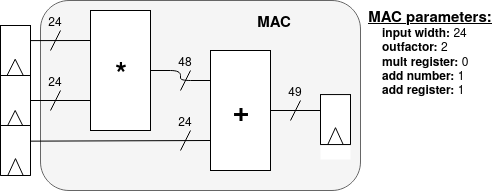
\includegraphics[width=0.7\textwidth]{Figures/Estimation-macro.png}
                \caption{Updated circuit from Figure \ref{ch.estimators:sec.resource-timing:ssec.basic:fig.estimation:sfig.mac} after macro recognition}
                \label{ch.estimators:sec.resource-timing:ssec.macro:fig.estimation:sfig.mac}
                \vspace{1em}
            \end{subfigure}
            \begin{subfigure}{1.0\textwidth}
                \centering
                \begin{adjustbox}{width=1.0\columnwidth,center}
                    \begin{tabular}{c|cc|cccc|c}
                        {\bf Operator/macro} & {\bf \#} & {\bf bit width} & {\bf LUT} & {\bf FF} & {\bf DSP} & {\bf BRAM} & {\bf Path (ns)}\\
                        \hline
                        {\tt MAC} [2, 0, 1, 1] & \ccg 1 & \ccg 24 & \ccg 40 & \ccg 0 & \ccg 3 & \ccg 0 & \ccg 3.821\\
                        {\tt REGISTER} & 3 & 24 & 0 & 24 & 0 & 0 & 0.695\\
                        \hline
                        {\bf Circuit} & \ccg ~ & \ccg ~ & \ccg 40 & \ccg 72 & \ccg 3 & \ccg 0 & \ccg 4.516\\
                    \end{tabular}
                \end{adjustbox}
                \caption{Macro based estimation of resource usage and critical path for Fig. \ref{ch.estimators:sec.resource-timing:ssec.macro:fig.estimation:sfig.mac} circuit}
                \label{ch.estimators:sec.resource-timing:ssec.macro:fig.estimation:sfig.results}
            \end{subfigure}
            \caption{Macro block based estimation methodology}
            \label{ch.estimators:sec.resource-timing:ssec.macro:fig.estimation}
        \end{figure}


        Using the macro block replacement technique to improve our basic estimation methodology enables better estimations of complex patterns, and thus better estimations of \firrtl{} circuits on \myAc{FPGA}.
        Figure \ref{ch.estimators:sec.resource-timing:ssec.macro:fig.estimation} enhances the estimation methodology exposed in Figure \ref{ch.estimators:sec.resource-timing:ssec.basic:fig.estimation} with macro block recognition and replacement.
        As macro blocks are parametrized by both {\bf generation} and {\bf configuration parameters}, we denote with {\tt MACRO} [$p_0$, ..., $p_{n-1}$] a {\bf macro block} with $n$ {\bf configuration parameters} $p_{x, x \in [\![0, n-1]\!]}$ in Figures \ref{ch.estimators:sec.resource-timing:ssec.macro:fig.estimation:sfig.lib} and \ref{ch.estimators:sec.resource-timing:ssec.macro:fig.estimation:sfig.results}.
        For example, the {\tt MAC} [2, 0, 1, 1] pattern represents a {\tt MAC} unit with an {\it outFactor} of 2, no {\tt REGISTER} after the {\tt MULT} operation, one {\tt ADD} operation and one {\tt REGISTER} after the computation. 
        As we can see, for a maximum {\it input bit width} of 16 bits, the whole pattern can be absorbed in only one \myAc{DSP}, while it would have taken one \myAc{DSP}, 32 \myAcs{LUT} and 33 \myAcs{FF} for the same pattern using only basic operator characterization.
        For the pattern introduced in Figure \ref{ch.estimators:sec.resource-timing:ssec.macro:fig.estimation:sfig.mac}, the estimations thus differ depending on the used methodology.


%%%%%%%%%%%%%%%%%%%%%%%%%%%%%%%%%%%%%%%%%%%%%%%%%%%%%%%%%%%%%%%%%%%%%%%%%%%%%%%%

% I'm so sorry
\vspace{-0.15cm}
\section{Quality of Service Estimation}
\label{ch.estimators:sec.qos}
\vspace{-0.1cm}

    Both timing and resources are key concerns when building hardware designs that target \myAcs{FPGA}, and should be considered in every design process.
    However, additional metrics should also be considered in specific use cases, as stated in Chapter \ref{ch.state}, and estimation methodologies should allow to easily integrate new metrics in order to be as flexible as possible.

    To demonstrate such flexibility, we chose to consider the \myLongAc{QoS}{Quality of Service} of circuits in our methodology, to demonstrate how additional estimators can be built and used in hardware design processes alongside resource and timing estimations.
    \myAc{QoS} is a main concern when it comes to particular domains such as \myLongAc{AxC}{Approximate Computing} or signal processing systems, as applications often require guarantees about the maximum error that may be introduced by approximations through computations.
    For example, usage of fixed point representations instead of IEEE-754 floating point numbers enable efficient hardware acceleration with no dedicated \myLongAc{FPU}{Floating-Point Unit}, but results in divergences with respect to the software computational model --- which often uses floating point representations as \myAcs{CPU} embed dedicated \myAc{FPU}.
    It is thus necessary to analyse the error introduced by such changes in the data representation to insure that acceleration does not provide erroneous results, in particular for critical systems.

    \subsection{Taxonomy of the Estimation Approaches}
    \label{ch.estimators:sec.qos:ssec.taxonomy}
    
        In order to build flexible estimators, we define a taxonomy for estimation methodologies and apply it to \myAc{QoS} estimation in Figure \ref{ch.estimators:sec.qos:ssec.taxonomy:fig.taxonomy}.
        An estimation can either be based on an analytic formula, an empirical approach, or both --- \eg when adding two fixed point numbers, one can consider the maximum error that may be generated, provide a statistical distribution of the two operands to derive an error model, or take an empirical approach and estimate the error by running multiple simulations.
        Each solution should be considered in this methodology to enable users to leverage their knowledge about the application domain and the target specificities --- \eg by making the decision to use \myAcs{FPU} if any are available on the target board.

        \begin{figure}[h!]
            \centering
            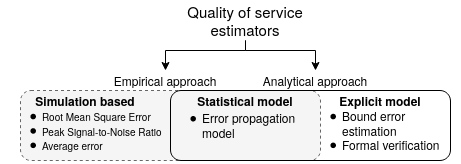
\includegraphics[width=1.0\textwidth]{Figures/taxonomy-qos.png}
            \caption{Taxonomy proposition for QoS estimators}
            \label{ch.estimators:sec.qos:ssec.taxonomy:fig.taxonomy}
        \end{figure}

    \subsection{Analytical Estimations}
    \label{ch.estimators:seq.qos:ssec.analytical}

        In order to provide analytical estimations for \myAc{QoS}, one should consider the specificities of both the data representation being used and the computations being performed.
        In most cases, a purely analytical approach is not desirable, as always considering the worst case for error propagation often results in inaccurate conclusions.
        For instance, knowing that an output on 8 bits with 4 bits of precision might have accumulated an error of $\pm 1/4$ does not bring any information on whether the implementation choices were good or not --- although can be used for critical system validation.
        Rather, statistical error propagation models can be used as basis to chose the data representation in a design, as assumptions on the statistical distributions of operands can help reduce the error propagation deduced from the analytical study of the system, and thus provide more relevant and exploitable results.

        In this context, we chose to enable users to define estimators at an analytical level, to derive \myAc{QoS} estimation from an expertise based analytical formula or error propagation models --- or any model based on analytical study of the design.
        Such estimators can use hardware generator parameters in analytical formulas, and should be achieved early in the flow, as they should not require further information about the circuit (see Section \ref{ch.estimators:sec.integration:ssec.multi-fidelity}).

    \subsection{Empirical Estimations}
    \label{ch.estimators:seq.qos:ssec.empirical}

        On the other hand, for non critical systems, an empirical approach may be used to provide \myAc{QoS} estimation, as occasional deviations for the expected behaviour should not have a noticeable impact on the design global \myAc{QoS} --- \eg occasional glitches in a video decoder are not as serious as erroneous results in the flight computer of plane.

\clearpage
        In this context, the users should be able to build estimators using simulation processes to bring information about empirical results.
        We thus integrate simulators in the estimation methodology, and propose helpers to build statistical analysis of empirical values to build significant estimators such as average error, standard deviation or \myLongAc{RMSE}{Root-Mean-Square Error} (which can be normalized).
        As a trade-off exists between the accuracy of an empirical estimator and the number of simulations to run, we expose the number of simulation runs as a parameter of the estimation process.

        After defining estimation methodologies for resource usage, critical paths and \myAc{QoS}, we then propose a generic way to integrate them in an \myAc{HCF}.

%%%%%%%%%%%%%%%%%%%%%%%%%%%%%%%%%%%%%%%%%%%%%%%%%%%%%%%%%%%%%%%%%%%%%%%%%%%%%%%%

\section[Integrating Metrics in a HCF]{Integrating Metrics in a Hardware\newline Construction Framework}
\label{ch.estimators:sec.integration}

    The main goal of this contribution is not to integrate a particular set of estimators to the chosen \myAc{HCF}, but rather to expose a generic \myAc{API} for users to define their own metrics and estimators with respect to their particular use cases.
    To do so, we propose a generic model for both metric definition and their integration in the framework, and apply them to the integration of estimators defined in Sections \ref{ch.estimators:sec.resource-timing} and \ref{ch.estimators:sec.qos}.

    \subsection{Exposing Multi-fidelity Estimators}
    \label{ch.estimators:sec.integration:ssec.multi-fidelity}
        In order to allow easy metric integration in the \chisel{} \myAc{HCF}, we start by defining abstraction levels where metric integration should be possible, as prior works exposed how {\bf multi-fidelity metrics} can be useful for exploration \cite{lo_multi-fidelity_2018} --- for it can enable either quick or accurate feedback depending on the needs and the exploration step.
    
        Figure \ref{ch.estimators:sec.integration:ssec.multi-fidelity:fig.flow} introduces the baseline \chisel{} development flow (Fig. \ref{ch.estimators:sec.integration:ssec.multi-fidelity:fig.flow:sfig.original}) and the proposed estimator integration steps (Fig. \ref{ch.estimators:sec.integration:ssec.multi-fidelity:fig.flow:sfig.proposed}).
        We choose to focus on three abstraction levels where estimators can be defined:
        \begin{itemize}
            \item Graph level --- \ie operating on \firrtl{} circuit representation
            \item Simulation level --- \ie using simulation results for estimation
            \item Register-Transfer level --- \ie calling \myAc{RTL} based external tools
        \end{itemize}

        As we can see on Figure \ref{ch.estimators:sec.integration:ssec.multi-fidelity:fig.flow:sfig.proposed}, the entry point of the flow is not altered with respect to the standard \chisel{} process (Fig. \ref{ch.estimators:sec.integration:ssec.multi-fidelity:fig.flow:sfig.original}).

\clearpage
        \begin{figure}[h!]
            \vspace{-0.1cm}
            \begin{subfigure}{0.49\textwidth}
                \centering
                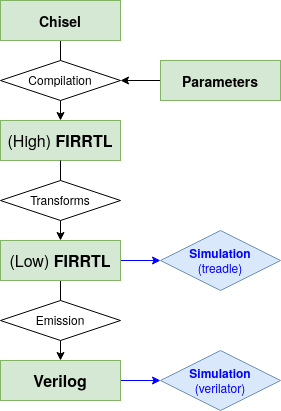
\includegraphics[width=0.75\textwidth]{Figures/chisel-flow-original.png}
                \vspace{3.5em}
                \caption{Chisel baseline development flow}
                \label{ch.estimators:sec.integration:ssec.multi-fidelity:fig.flow:sfig.original}
            \end{subfigure}
            ~
            \begin{subfigure}{0.49\textwidth}
                \centering
                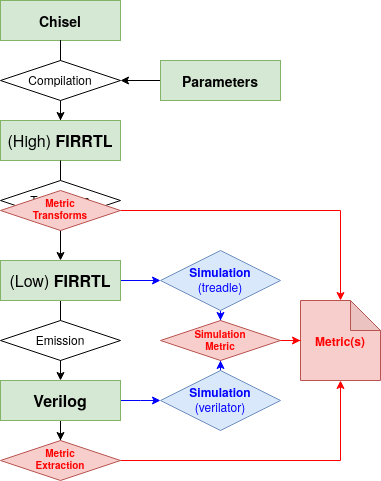
\includegraphics[width=1.0\textwidth]{Figures/chisel-flow-proposed.png}
                \caption{Integration of multi-fidelity metric in chisel development flow}
                \label{ch.estimators:sec.integration:ssec.multi-fidelity:fig.flow:sfig.proposed}
            \end{subfigure}
            \caption{Proposition for \chiselT{} flow enhancement}
            \label{ch.estimators:sec.integration:ssec.multi-fidelity:fig.flow}
            \vspace{-0.2cm}
        \end{figure}

        The {\bf graph level} estimators are then built by adding some custom transforms to the ones that are used by \chisel{} to produce a low \firrtl{} representation, while the {\bf simulation level} estimators are build by exposing an interface with the different {\bf simulation backends} that are integrated in \chisel{} and operate either at \firrtl{} level or on the generated \verilog.
        For readability purposes, we only expose the two main backends integrated in \chisel: \treadle{}, which is specific for \chisel{} and directly operate on the low \firrtl{} representation, and \verilator, which is an open-source tool that uses C++ for efficient cycle-accurate simulations.
        However, other simulators can be integrated as well, as long as they can be interfaced with one of the different representations at stake in the flow.
        Finally, the \myAc{RTL} estimators are integrated through the usage of the file system, and can rely on any tool that can take the generated \verilog{} descriptions as its entry points.

        Using those three abstraction levels, one can adjust both estimation \myAc{QoR} and speed for their custom flows in a generic way --- for example, both resource and timing estimators from Section \ref{ch.estimators:sec.resource-timing} are integrated at graph level, while \myAc{QoS} estimators from Section \ref{ch.estimators:sec.qos} are integrated either at simulation level or at graph level.
        The reference values that are computed through the syntheses are integrated at \myAc{RTL} level, showing that a classical design flow can also be achieved through this \myAc{API}.

\clearpage
    \subsection[Proposed Application Programming Interface]{Proposed {\it Application Programming Interface}}
    \label{ch.estimators:sec.integration:ssec.api}

        In order to integrate our estimation methodology in \chisel{} \myAc{HCF}, we propose to use the {\bf \firrtl{} transform system}, which is used by the framework to enable optimization and circuit generation through \myAc{IR} scans, as shown in Figure \ref{ch.estimators:sec.integration:ssec.multi-fidelity:fig.flow}.
        In fact, we define three levels for the integration:
        \begin{itemize}
            \item {\bf pre-elaboration} level --- which does not require \myAc{RTL} generation (\eg analytical approach)
            \item {\bf elaboration} level --- which operates on \firrtl{} representations (\eg resource and timing estimation)
            \item {\bf post-elaboration} level --- which operates after \myAc{RTL} generation (\eg simulation and syntheses)
        \end{itemize}
        
        {\bf Pre-elaboration} estimations are performed directly on the generator, by extracting metric estimations from constructor parameters, while {\bf post-elaboration} estimations are run at the end of the \myAc{HCF} process, and may leverage external tools such as synthesis suits or simulators.
        As for {\bf elaboration} estimators, they are integrated directly in the \firrtl{} flow, and uses the inner transform and annotation system --- which consists in a sequence of transforms operating on a circuit representation, which can modify it and/or use an annotation system to forward information in the flow --- to generate estimations from \myAc{IR} scans and forward it to the rest of the flow through annotation usage.

        At the end of an estimation run, all the estimated metrics can be collected from the annotation system, and used by the developers to iterate on their designs until a satisfying solution is found.

%%%%%%%%%%%%%%%%%%%%%%%%%%%%%%%%%%%%%%%%%%%%%%%%%%%%%%%%%%%%%%%%%%%%%%%%%%%%%%%%

\clearpage
\section[Synthesis on the Estimation Methodologies]{Synthesis on Estimation Methodologies}
\label{ch.estimators:seq.synthesis}

    In this chapter, we discussed the importance of qualitative estimations for hardware development processes, and put a particular focus on their application for \myLongAc{DSE}{Design Space Exploration}.

    We considered three different types of metric to be estimated --- namely resource usage, maximum operating frequency and \myAc{QoS} --- as well as how they can be estimated at different levels of fidelity.
    We proposed a simple estimation methodology based on an \myLongAc{IR}{Intermediate Representation} analysis for both spatial and temporal concerns, as well as an estimation taxonomy for \myLongAc{QoS}{Quality of Service} metrics, focusing on the \myLongAc{AxC}{Approximate Computing} domain.

    We then introduced a generic \myLongAc{API}{Application Programming Interface} integrated in the \chisel{} \myLongAc{HCF}{Hardware Construction Framework} to allow users to define their own metrics and estimators.
    This interface is supposed to be comprehensive enough to allow any user to leverage the \firrtl{} representation system to define their custom metrics.
    
    As the \myLongAc{QoR}{Quality of Results} of estimators is a main focus when it comes to \myAc{DSE}, various metrics and estimators will be considered in the next section, which will focus on building an exploration framework integrated in a \myAc{HCF}.

%%%%%%%%%%%%%%%%%%%%%%%%%%%%%%%%%%%%%%%%%%%%%%%%%%%%%%%%%%%%%%%%%%%%%%%%%%%%%%%%%
%%%%%%%%%%%%%%%%%%%%%%%%%%%%%%%%%%%%%%%%%%%%%%%%%%%%%%%%%%%%%%%%%%%%%%%%%%%%%%%

\cleardoublepage
%-------------------------------------------------------------------------------
\chapter{Design Space Exploration Methodology}
\labelchapter{ch.dse}
%-------------------------------------------------------------------------------

%%%%%%%%%%%%%%%%%%%%%%%%%%%%%%%%%%%%%%%%%%%%%%%%%%%%%%%%%%%%%%%%%%%%%%%%%%%%%%%%
%%%%%%%%%%%%%%%%%%%%%%%%%%%%%%%%%%%%%%%%%%%%%%%%%%%%%%%%%%%%%%%%%%%%%%%%%%%%%%%%

\lettrine[lines=2]{A}{fter} defining the interest of relevant metrics and accurate estimators for hardware development processes, we focus on their usage for \myLongAc{DSE}{Design Space Exploration}.
This chapter outlines the specificities of \myLongAcs{HCL}{Hardware Construction Language} that can be used for efficient \myAc{DSE}, before proposing a methodology for \myAc{HCL}-based \myAc{DSE}.
This methodology is based on high level programming features such as \myLongAc{OOP}{Object-Oriented Programming} or functional programming, which enable more expressivity for the developers.
We also exhibit the limitations of this approach and discuss various solutions to improve the proposed methodology.

\vspace*{\fill}
\minitoc 
\mtcskip 

\newpage
%%%%%%%%%%%%%%%%%%%%%%%%%%%%%%%%%%%%%%%%%%%%%%%%%%%%%%%%%%%%%%%%%%%%%%%%%%%%%%%%

\section[Defining DSE in a HCL context]{Defining Design Space Exploration using Hardware Construction Languages}
\label{ch.dse:sec.definition}

    This section aims at defining how \myLongAcs{HCL}{Hardware Construction Language} specificities can be leveraged for efficient \myLongAc{DSE}{Design Space Exploration}, in contrast to other \myAc{DSE} methodologies based on various paradigms.

    The \myAc{HCL} paradigm enables to describe hardware circuit generators instead of hardware circuits, allowing to fully control generated hardware at \myLongAc{RTL}{Register-Transfer Level}.
    Doing so, we can define \myAc{DSE} methodologies which leverage the developers expertise to reduce the amount of implementations to explore, as some of them can easily be pruned considering prior knowledge on both algorithm and target.
    Moreover, high level features such as \myLongAc{OOP}{Object-Oriented Programming} or functional programming can be used to expose variations, exposing more complex implementation options --- such as the definition of various computation units using functions as module parameters --- when compared to standard \myAc{DSE} flows, such as \myLongAc{HLS}{High Level Synthesis} methodologies.

    \subsection{Meta Design and Meta Exploration}
    \label{ch.dse:sec.definition:ssec.meta}
        In order to propose an efficient \myAc{HCL}-based \myAc{DSE} methodology, we start by defining two main concepts: {\bf meta design} and {\bf meta exploration}.

        {\bf Meta design} is defined as the process of building an explorable design generator based on a prior analysis of both algorithm and target (Fig. \ref{ch.dse:sec.definition:ssec.meta:fig.meta-design}).
        Leveraging this analysis, a developer can define relevant implementation variations --- meaning that each possible implementation results from a choice from the user --- and expose them at top level, directly in the module constructor.
        Doing so, the exploration process no more relies on tool inferences to generate such variations --- \eg as it is the case with \myAc{HLS} methodologies --- but on controlled variations of the generators, resulting in a more meaningful design space to be explored.
        Moreover, using such methodologies enable a more intelligible approach of the exploration, as the implementation options are directly defined by users, enabling a better apprehension of their impacts on the generated design.
        
        \begin{figure}[h!]
            \centering
            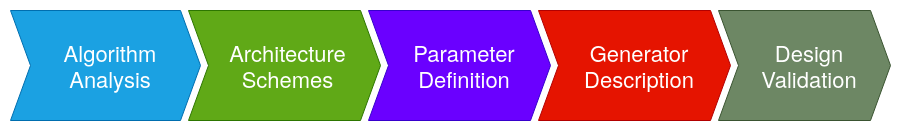
\includegraphics[width=0.9\textwidth]{Figures/Methodology-metadesign}
            \caption{Meta design methodology}
            \label{ch.dse:sec.definition:ssec.meta:fig.meta-design}
        \end{figure}

\clearpage
        We then define {\bf meta exploration} (Fig. \ref{ch.dse:sec.definition:ssec.meta:fig.meta-exploration}) as a process exploiting a design generator --- that was built using {\bf meta design} --- to explore its implementation variations, thus defining a \myAc{HCL}-based \myAc{DSE} methodology.
        In order to provide efficient exploration processes, this methodology allows the users to define custom strategies --- after defining the design space --- leveraging their expertise to guide the flow.
        In the next sections, we will consider a strategy to be composed of various metrics to be estimated (with respect to the considerations introduced in Chapter \ref{ch.estimators}), as well as the different steps to browse the design space (see Section \ref{ch.dse:sec.functional}).
        \begin{figure}[h!]
            \centering
            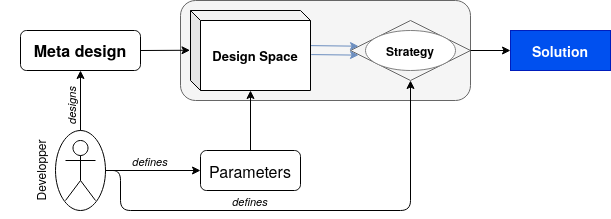
\includegraphics[width=1.0\textwidth]{Figures/Methodology-metaexploration}
            \caption{Meta exploration methodology}
            \label{ch.dse:sec.definition:ssec.meta:fig.meta-exploration}
        \end{figure}

    \subsection{Implementation Knobs and Parameters}
    \label{ch.dse:sec.definition:ssec.knobs}

        As seen in Section \ref{ch.state:sec.space:ssec.mixing}, \myAc{HLS} and \myLongAcs{DSL}{Domain Specific Language} based \myAc{DSE} methodologies are based on {\bf knobs} --- \ie implementation options --- which can be of three kinds: local attributes (as pragmas), global synthesis options and \myLongAcs{FU}{Functional Unit} options \cite{schafer_high-level_2020}.

        The exploration knobs are used by \myAc{DSE} tools to generate implementation variations, resulting in an explorable space of equivalent implementations of a same algorithm.
        It is thus comparable to the parameters of {\bf meta design} based circuit generators as defined in Section \ref{ch.dse:sec.definition:ssec.meta}.

        However, the high level parameters exposed by the {\bf meta design} methodology cannot express global synthesis options as it is done with knobs, and such variations must thus be considered in the {\bf meta exploration} strategy, in order to offer comparable features.
        Nevertheless, both local attributes and \myAc{FU} options can be leveraged using design generator parameters, and will then be used in this work to define explorable design spaces.

%%%%%%%%%%%%%%%%%%%%%%%%%%%%%%%%%%%%%%%%%%%%%%%%%%%%%%%%%%%%%%%%%%%%%%%%%%%%%%%%%

\section{Building Explorable Architectures}
\label{ch.dse:sec.explorable}
    As defined in the previous section, the first step to define our \myAc{HCL}-based \myAc{DSE} methodology is to build an efficient {\bf meta design} method.

    \subsection{Designing Explorable Hardware Generators}
    \label{ch.dse:sec.explorable:ssec.generators}
        To design explorable hardware generators, one should begin by analysing both the algorithm and the target to exhibit meaningful implementation variations.
        It should result in a design space of relevant architectures to be explored, while leveraging the users expertise to expose both specific and non specific parameters.

        For example, the \myLongAc{IO}{Input/Output} bandwidth is a non specific parameter, as it will have a significant impact on most of circuits, while the potential of parallelism or the number of a particular \myAc{FU} in a given architecture is application specific, as it will not have the same impact nor the same definition, depending on the targeted algorithm.
        The user expertise is thus required to produce a good analysis, and is primordial for this whole methodology to produce meaningful results.

        After defining the exploration parameters, one needs to exhibit the possible values for each of them, in order to build the design space --- \ie a set of parameters which will be used in elaboration to give a particular implementation.
        For each parameter, users thus need to define a set of possible values, and each set is then considered in a {\bf cartesian product} to build the resulting design space.

        In order to integrate the {\bf meta design} methodology in an \myLongAc{HCF}{Hardware Construction Framework}, we propose to expose both parameters and their values at circuit top levels, in order to build intelligible flows and allow easy evolutions of the exploration processes.

        \begin{figure}[h!]
            \begin{lstlisting}[xleftmargin=0mm,
                               caption={Exposing the dot product design space},
                               label={ch.dse:sec.explorable:ssec.generators:list.dotproduct}]
class DotProduct(
  @linear(6, 12)    dynamic: Int,
  @linear(6, 12)    precision: Int,
  @enum(16)         nElem: Int,
  @linear(0, 4)     parallelism: Int
) extends Module with Explorable\end{lstlisting}
        \end{figure}

\clearpage
        In Listing \ref{ch.dse:sec.explorable:ssec.generators:list.dotproduct}, we use \chisel{} constructors to expose the design space of a {\bf dot product} design, computing the dot product of two vectors $a_n$ and $b_n$.\footnote{Given $a_n = (a_0, ..., a_{n-1})$ and $b_n = (b_0, ..., b_{n-1})$, we compute $c = \sum_{i = 0}^{n-1} a_i * b_i$.}
        
        We define four different parameters, namely the element dynamic and precision in bits (as the circuit only consider fixed point elements), the number of elements in each vector and the level of parallelism.

        For each parameter, we only consider integer values for simplicity purpose, and define different set generators in Figure \ref{ch.dse:sec.explorable:ssec.generators:fig.annotations}.
        \begin{figure}[ht!]
            \centering
            \begin{itemize}
                \item \lstinline{@byX(x, y)} $\Leftrightarrow$\hspace*{\fill}$p \in [\![x, y]\!] \land p \equiv 0 \pmod X$
                \item \lstinline{@linear(x, y)}\footnotemark$\Leftrightarrow$\hspace*{\fill}$p \in [\![x, y]\!]$
                \item \lstinline{@enum(x0, ..., xn)} $\Leftrightarrow$ \hspace*{\fill} $p \in \{x_0, ..., x_n\} \land \forall i \in [\![0, n]\!], x_i \in \mathbb{N}$
                \item \lstinline{@powX(x, y)} $\Leftrightarrow$\hspace*{\fill}$p \in \mathbb{N}/p = X^z \land z \in [\![x, y]\!]$
                \item \lstinline{@pow2(x, y)} $\Leftrightarrow$\hspace*{\fill}$p \in \mathbb{N}/p = 2^z \land z \in [\![x, y]\!]$
            \end{itemize}
            \caption{Annotation based parameter generation}
            \label{ch.dse:sec.explorable:ssec.generators:fig.annotations}
        \end{figure}
        \footnotetext[\thefootnote]{Equivalent to \lstinline{@by1(x, y)}.}

        We use the \scala{} annotation system to directly annotate the constructor parameters with value generators, thus embedding both parameters and their values in the top level module --- \ie the entry point of the \chisel{} flow.

        For the {\bf dot product} algorithm, we thus build a $7 \times 7 \times 1 \times 5 = 245$ wide design space to be explored, using the cartesian product of each set of possible values: both {\it dynamic} and {\it precision} can each take $|[\![6, 12]\!]| = 7$ different values, while {\it parallelism} can take 5, and {\it nElem} is fixed.

    \subsection{Impact of the Implementation Parameters}
    \label{ch.dse:sec.explorable:ssec.impact}
        This approach allows to define the design space in an easy way by integrating it directly in the top level module, through its constructor.

        However, leveraging the user expertise is not only about defining meaningful parameters and their values for the exploration, but also about bringing information about how the parameter variations may impact the exploration processes.
        For example, in the {\bf dot product} implementations, we can state that the three first parameters --- namely {\it dynamic}, {\it precision} and {\it nElem} --- impact the algorithm \myLongAc{QoS}{Quality of Service}, while the fourth one --- {\it parallelism} --- does not, as it only impacts the latency of the generated circuit.

        In order to improve this first approach with respect to this observation, we thus need a way to define if a particular parameter variations has an impact on a given metric.
        With such feature, a given exploration step that considers only the \myAc{QoS} of the designs will not consider the fourth dimension of the {\bf dot product} generator, as every variation of the fourth parameter in the design space is to be considered equivalent with respect to the \myAc{QoS}.
        This enables to reduce the design space, dividing the number of implementations to explore by a factor 5 --- the cardinality of the {\it parallelism} set of values --- for an exhaustive exploration process.

    \subsection[Exposing an Expertised Based Design Space]{Exposing an Expertise Based Design Space for Exploration}
    \label{ch.dse:sec.explorable:ssec.space}

        In order to enhance design space with informations on how chosen parameters impact given metrics, we add yet another annotation system to module constructors, in a way similar to the one introduced in Section \ref{ch.dse:sec.explorable:ssec.generators}.
        We thus add a \lstinline{@qualityOfService} annotation, which bears the information that the annotated parameter does impact the \myAc{QoS} metric.

            \begin{figure}[h!]
                \vspace{-0.2cm}
                \begin{lstlisting}[xleftmargin=0mm,
                                   caption={[Enhancing the dot product design space]Enhancing the dot product design space with quality of service\newline concerns},
                                   label={ch.dse:sec.explorable:ssec.space:list.dotproduct}]
class DotProduct(
  @qualityOfService @linear(6, 12)  dynamic: Int,
  @qualityOfService @linear(6, 12)  precision: Int,
  @qualityOfService @enum(16)       nElem: Int,
                    @linear(0, 4)   parallelism: Int
) extends Module with Explorable\end{lstlisting}
                \vspace{-0.5cm}
            \end{figure}

        For the dot product example, Listing \ref{ch.dse:sec.explorable:ssec.space:list.dotproduct} shows how new information can be brought about built design space: by specifying that only 3 of 4 parameters have an impact on circuit \myAc{QoS}, we then reduce the design space from {\bf 245} to {\bf 49 different implementations} to be explored for explorations focusing on such concerns.

%%%%%%%%%%%%%%%%%%%%%%%%%%%%%%%%%%%%%%%%%%%%%%%%%%%%%%%%%%%%%%%%%%%%%%%%%%%%%%%%%

\section[On Functional Programming for DSE]{On Functional Programming for Design Space Exploration}
\label{ch.dse:sec.functional}

    Using high level languages such as \scala{} enables leveraging features such as \myAc{OOP} or {\bf functional programming} for hardware generation.
    However, as such features are directly integrated in the \myAc{HCF}, they can also be used for side functionalities beside hardware elaboration.

    In order to demonstrate how high level features can be used to improve hardware developers life, we build a \myAc{DSE} methodology based on functional programming.

    \subsection{Mathematical Formalization}
    \label{ch.dse:sec.functional:ssec.formalization}

        In this section, we formalize how functional programming can be used to define \myAc{DSE} strategies, and expose a methodology based on this formalism. 

        \subsubsection{Theoretical basis}
    
            Let $\cal{A}$ be an input vocabulary, which will be used to define metric names.
            We define $\cal{M}_{\cal{A}} = \cal{A} \times \mathbb{R}$ the set of {\bf named metrics} with values in $\mathbb{R}$, representing any metric in an exploration process.

            Metrics can be of two kinds: they either refer to the implementation parameters that were exposed through the {\bf meta design} methodology, or they represent objective and constraint metrics that were generated during prior exploration steps.
            {\bf Named metrics} are thus pairs of the form $(name, value)$, such as $(dynamic, 12.0)$ or $(frequency, 275.96)$.

            Let $n \in \mathbb{N^*}$, we define a {\bf configuration of order n} --- \ie a configuration relying on {\bf n named parameters}%
            \footnote{{\bf Named parameters} are a special case of {\bf named metrics}, as they will represent not only metrics (\ie design properties) but also coordinates in the {\bf design spaces} that will be defined in this section.} %
            --- as $x_n = \{x_0, ..., x_{n-1}\}$, with $x_i \in \cal{M}_{\cal{A}}$ and $i \in [\![0, n-1]\!]$.
            Each configuration stands for a different implementation variation, and we hence define a design space as being all the possible implementations for a given {\bf meta design}.

            We then define a {\bf point of order (n, k)} as being an improved configuration, bearing both the configuration parameters $x_i$ with $i \in [\![0, n-1]\!]$ and some generated metrics $m_i$ with $i \in [\![0, k-1]\!]$.
            A point $p_{(n, k)}$ can then be defined as a vector of elements in $\cal{M}_{\cal{A}}$ which characterizes a given implementation: 
            \begin{equation}
                \label{ch.dse:sec.functional:ssec.formalization:eq.point}
                p_{(n, k)} = \{\underbrace{x_0, ..., x_{n-1}}_{n\: \text{parameters}}, \underbrace{m_0, ..., m_{k-1}}_{k\: \text{metrics}}\}
            \end{equation}

            Using such definition, we characterize a {\bf design space of order n} as being a {\bf set of points of order n}, denoted as being $s_n = \{p_{(n, \_)}\}$.
            We only consider the number of parameters for each configuration to define the dimensions of a design space, as the metrics do not represent dimensions but only information on the designs.
            For generalization purposes, we define $\mathbb{S}_n$ as being the set of all the possible exploration spaces $s_n$.

   
\clearpage
            We now aim at defining {\bf design space exploration strategies} operating on so defined design spaces.
            We start by defining {\bf cost functions $c$} as a way to generate new {\bf named metrics} in $\cal{M}_{\cal{A}}$:
            \begin{equation}
                \label{ch.dse:sec.functional:ssec.formalization:eq.costFunction}
                \begin{split}
			c: {\cal{M}_{\cal{A}}}^{n+k} & \rightarrow {\cal{M}_{\cal{A}}}\\
			p_{(n,k)} & \mapsto c(p_{(n,k)})
                \end{split}
            \end{equation}
            
            Using so-built cost functions, we define {\bf estimation transforms of order $\theta$}, which are used to enhance a given design space with {\bf $\theta$ new metrics}.
            Given {\bf $\theta$ cost functions} $c_i$ with $i \in [\![0, \theta-1]\!]$, an estimation transform $f_\theta$ operating over points $p_{(n, k)}$ is defined as follows:
            \begin{equation}
                \label{ch.dse:sec.functional:ssec.formalization:eq.estimationTransform}
                \begin{split}
                    f_\theta: {\cal{M}_{\cal{A}}}^{n+k} & \rightarrow {\cal{M}_{\cal{A}}}^{n+k+\theta}\\
                    p_{(n, k)} & \mapsto p_{(n, k + \theta)}
                \end{split}
            \end{equation}
            The resulting points are thus enhanced with $\theta$ new {\bf named metrics}:
            \begin{equation}
                \label{ch.dse:sec.functional:ssec.formalization:eq.enhancedPoint}
                \begin{split}
                    p_{(n, k + \theta)} &= \{x_0, ..., x_{n-1}, m_0, ..., m_{k-1}, c_0(p_{(n, k)}), ..., c_{\theta-1}(p_{(n, k)})\}\\
                                       &= \{\underbrace{x_0, ..., x_{n-1}}_{n\: \text{parameters}}, \underbrace{m_0, ..., m_{k-1}}_{k\: \text{old metrics}}, \underbrace{m_k, ..., m_{k+\theta-1}}_{\theta\: \text{new metrics}}\}
                \end{split}
            \end{equation}


            We define a {\bf morphism} as a modification of a {\bf design space of order $n$}, which can be a way to sort, prune or even enhance it --- and we call $\mathbb{M}_n$ the set of all the possible {\bf morphisms} of order n.
            A {\bf morphism} can also modify the dimensions of the {\bf design space}, hence changing the number of {\bf points} to be explored:
            \begin{equation}
                \label{ch.dse:sec.functional:ssec.formalization:eq.morphism}
                \begin{split}
                    m_n: \mathbb{S}_n & \rightarrow \mathbb{S}_{n'}\\
                    s_n & \mapsto s_{n'}'
                \end{split}
            \end{equation}

            We finally define how the {\bf estimation transforms} are to be applied over a design space, before potentially modifying it through a {\bf given morphism}.
            
            Considering an estimation transform $f_\theta$ of order $\theta$, a morphism $\mu_n$ of order n, and an input {\bf design space} $s_n$ of order n, we define a {\bf transform application function} of order $(n, \theta)$ as being:
            \begin{equation}
                \label{ch.dse:sec.functional:ssec.formalization:eq.application}
                \begin{split}
                    a_{(n, \theta)}: \mathbb{F}_\theta \times \mathbb{M}_n \times \mathbb{S}_n & \rightarrow \mathbb{S}_{n'}\\
                    (f_\theta, \mu_n, s_n) & \mapsto \mu_n(\{f_\theta(p_{(n, k)})\}) \: \text{with} \: p_{(n,k)} \in s_n  
                \end{split}
            \end{equation}
            It is important to remark that one cannot presume about how the morphism and the estimation transform are applied over the input design space, and how they interact together.
            For example, the estimation transform can be applied to all the points in the design space before applying a modification of its structure, or it can be applied through a more selective approach, for example using a gradient descent algorithm.
            In the following of this work, we will denote the set of all the possible {\bf transform application functions} of order $(n, \theta)$ as $\mathbb{A}_{(n, \theta)}$.

            For a more concise writing, we will use the {\bf currying} notion, which is used in the {\bf functional programming paradigm}.
            It refers to the action of converting a function with multiple arguments to a parametrized functions, which only takes one argument.
            For example, a function $f(a, b)$ can be converted to a set of functions $f(a)$, which can then be applied to the second argument, $b$.

            We will hence convert our {\bf transform application functions} to be simple functions operating over an input {\bf design space}:
            \begin{equation}
                \begin{split}
                \label{ch.dse:sec.functional:ssec.formalization:eq.app}
                    a_{(n, \theta)}(f_\theta, \mu_n, s_n) \Rightarrow a_{(n, \theta)}(f_\theta, \mu_n)(s_n) = \alpha_{(f_\theta, \mu_n)}(s_n)
                \end{split}
            \end{equation}

            Using all those constructs, we define an {\bf exploration step} as a {\bf function} operating over a {\bf design space} by applying, given some {\bf transform application function}, a set of {\bf estimation transforms} to the {\bf points} composing the space, before modifying its structure using a given {\bf morphism}, and returning a new space enhanced with {\bf new metrics}.
            More formally, we define an exploration step as being:
            \begin{equation}
                \label{ch.dse:sec.functional:ssec.formalization:eq.exploration}
                \begin{split}
                    e: \mathbb{M}_{n'} \times \mathbb{A}_{(n, \theta)} \times \mathbb{S}_n & \rightarrow \mathbb{S}_{n''}\\
                    (m_{n'}, \alpha_{(f_\theta, \mu_n)}, s_n) & \mapsto m_{n'}(\alpha_{(f_\theta, \mu_n)}(s_n))
                \end{split}
            \end{equation}

            Doing so, we can use {\bf currying} once again, to define {\bf exploration steps} as being simple functions operating over {\bf design spaces}:
            \begin{equation}
                \label{ch.dse:sec.functional:ssec.formalization:eq.explo}
                \begin{split}
                    e(m_{n'}, \alpha_{(f_\theta, \mu_n)}, s_n) \Rightarrow \epsilon_{(m_{n'}, \alpha)}(s_n)
                \end{split}
            \end{equation}

            We finally use {\bf functional programming} to compose basic strategies and build more complex ones, by applying $n$ exploration strategies $[\![\epsilon_0, ..., \epsilon_{n-1} ]\!]$ in a sequential way over an initial {\bf design space}.

        \subsubsection{Basic functions for a concise definition of the exploration steps}
            In order to take the best of the functional programming paradigm for \myAc{DSE}, we provide some basic functions for a concise description of some popular programming patterns.
            For each introduced function, we will propose multiple equivalent descriptions --- which are more or less compact and understandable --- to help the user to understand how this emerging paradigm can be used for \myAc{DSE}.

\clearpage
            First of all, we consider the {\bf map-reduce} pattern, where a function is applied to every element in a given sequence, before performing a reduction to return only one value.
            For example, considering a vector of elements $e_i$, $i \in [\![0, k]\!]$, one can use this pattern to compute a sum of squares:%
            \footnote{In this context, we will use some simplification coming for the functional programming paradigm, to replace implicit parameters (\eg x) by a simple placeholder \_, when there is no ambiguity for the compiler.}
            \begin{equation}
                \label{ch.dse:sec.functional:ssec.formalization:eq.mapreduce}
                \begin{split}
                    sum &= e.map(x \Rightarrow x^2).reduce((a, b) \Rightarrow a+b)\\
                        &= e.map(\_^2).reduce(\_+\_)\\
                        &= e.map(square).reduce(add)\\
                        \text{with}\: &square(x) = x^2 \: \text{and} \: add(a, b) = a+b
                \end{split}
            \end{equation}

            We will also use some simple operations over the collections, for example the {\tt sortWith} function, which operates over a collection {\tt col} and sort its elements by applying a comparison function.
            For example, if we want to sort a collection {\tt col} of objects using a particular attribute {\tt .value}, we can use:
            \begin{equation}
                \label{ch.dse:sec.functional:ssec.formalization:eq.sortwith}
                \begin{split}
                    newCol &= col.sortWith((a, b) \Rightarrow a.value \leq b.value)\\
                           &= col.sortWith(\_.value \leq \_.value)\\
                           &= col.sortWith(compare)\\
                       \text{with}\: &compare(a, b) = a.value \leq b.value
                \end{split}
            \end{equation}

            Another useful operation is about filtering a collection, using a boolean function --- \eg to select only the elements for which the {\tt .value} attribute is above a threshold $min_{value}$:
            \begin{equation}
                \label{ch.dse:sec.functional:ssec.formalization:eq.filter}
                \begin{split}
                    newCol &= col.filter(x \Rightarrow x.value > min_{value})\\
                           &= col.filter(\_.value > min_{value})\\
                           &= col.filter(func)\\
                       \text{with}\: &func(x) = x.value > min_{value}
                \end{split}
            \end{equation}

            With respect to the formalism introduced in the previous section, we can remark that {\tt sortWith}, {\tt map} and {\tt filter} can be defined as {\bf morphisms}, if the collection {\tt col} is a design space.
            As those constructs do not modify the number of {\bf parameters} in the points they are operating on, they can even be considered as {\bf endomorphisms} --- \ie morphisms from $\mathbb{S}_n$ to $\mathbb{S}_n$.

            In the following section, we will then use a compact description of the different functions to be applied on the design spaces, to exhibit how the {\bf functional programming paradigm} can help users to define concise yet intelligible exploration strategies.

\clearpage
        \subsubsection{Application examples}
            As an example, we define {\bf exhaustive strategies}, where the {\bf transform application function} (from Eq. \ref{ch.dse:sec.functional:ssec.formalization:eq.app}) consists in an exhaustive application of the {\bf estimation transform} to all the {\bf points} in the {\bf design space}:
            \begin{equation}
                exhaustive_{(m_n, f_\alpha)}(s_n) = m_n(s_n.map(f_\alpha)))
            \end{equation}

            It can be applied to define {\bf exhaustive sort}, based on a comparison function $cmp$ used to define an {\bf order} over a {\bf design space $s_n$}:
            \begin{equation}
                \label{ch.dse:sec.functional:ssec.formalization:sssec.application:eq.sort}
                \begin{split}
                    sort_{(f_\alpha, cmp)}(s_n) &= exhaustive_{(sortWith(cmp), f_\alpha)}(s_n)\\
                                              &= s_n.map(f_k).sortWith(cmp)
                \end{split}
            \end{equation}
            
            We also define {\bf exhaustive pruning} of the space, using a pruning function $f_{prune}$ to specify which {\bf points} are to be left in the resulting design space:
            \begin{equation}
                \label{ch.dse:sec.functional:ssec.formalization:sssec.application:eq.prune}
                \begin{split}
                    prune_{(f_\alpha, f_{prune})}(s_n) &= exhaustive_{(filter(f_{prune}), f_\alpha)}(s_n)\\
                                                       &= s_n.map(f_\alpha).filter(f_{prune})
                \end{split}
            \end{equation}

            Based on those two basic strategies, we can define a more complex one, which uses both quick metric generation through \myAc{RTL} estimations of the resources, and accurate estimations through synthesis processes.

            To do so, we define a first strategy $\epsilon_0$ which we will refer too as the {\it preliminary pruning}, and a second one, $\epsilon_1$, that will be referred as the {\it refinement}.
            We define $estim$ as a {\bf cost function} of order 1, based on a \myAc{RTL} estimation of the \myAc{LUT} resource usage, producing a metric of named $LUT_{estim}$ for a given circuit.
            We also define $synth$ as another {\bf cost function} of order 1, based on an external synthesis tool call, producing a metric named $LUT_{synth}$, which is the reference value that the \myAc{LUT} estimation should approximate.
            
            $\epsilon_0$ is thus defined as follow, considering a threshold $t_{max}$ which represents the maximum amount of \myAcs{LUT} acceptable in an implementation:
            \begin{equation}
                \begin{split}
                    \epsilon_0(s_n) & = prune_{(estim, \_.LUT_{estim} < t_{max})}(s_n) \\
                                    & = s_n.map(estim).filter(\_.LUT_{estim} < t_{max})
                \end{split}
            \end{equation}

            \noindent As for $\epsilon_1$, it is defined as:
            \begin{equation}
                \begin{split}
                    \epsilon_1(s_n) & = sort_{(synth, \_.LUT_{synth} > \_.LUT_{synt})}(s_n) \\
                                    & = s_n.map(synth).sortWith(\_.LUT_{synth} > \_.LUT_{synth})
                \end{split}
            \end{equation}
            
            \noindent The global {\bf exploration strategy} $\epsilon_\tau = \epsilon_0 \circ \epsilon_1$ can hence be defined as:
            \begin{equation}
                \label{ch.dse:sec.functional:ssec.formalization:sssec.application:eq.tau}
                \begin{split}
                    \epsilon_\tau(s_n) = s_n&.map(estim).filter(\_.LUT_{estim} < t_{max})\\
                                            &.map(synth).sortWith(\_.LUT_{synth} > \_.LUT_{synth})
                \end{split}
            \end{equation}

\clearpage
        This methodology hence enables to describe and compose {\bf exploration strategies} in a functional way, as each can be considered as a simple function over a {\bf design space}.
        Moreover, each strategy can itself be defined in a functional way, as it is mainly defined as a combination of various {\bf estimation transforms} and some {\bf morphisms} to be applied to a given {\bf design space}.

    \subsection{Basic Exploration Strategies}
    \label{ch.dse:sec.functional:ssec.basic}

        To demonstrate how the defined methodology can be used by hardware developers to leverage their expertise and build intelligent {\bf exploration strategies}, we propose to implement five {\bf basic strategies} as a {\it proof of concept}:
        \begin{enumerate}
            \setlength\itemsep{-.4em}
            \item exhaustive sort of the space (Eq. \ref{ch.dse:sec.functional:ssec.formalization:sssec.application:eq.sort})
            \item exhaustive pruning of the space (Eq. \ref{ch.dse:sec.functional:ssec.formalization:sssec.application:eq.prune})
            \item explicit dimension removal, based on the user knowledge
            \item gradient descent search over the space (Algo. \ref{ch.dse:sec.functional:ssec.basic:algo.gradient})
            \item quick pruning through frontier approximation (Algo. \ref{ch.dse:sec.functional:ssec.basic:algo.quick})
        \end{enumerate}

        The first two strategies have already been defined in the previous section, and will be used as basic elements for more complex strategy building --- as they rely on the exhaustive application of a given function to the explored design space, their implementation can be trivially based on any high level language featuring functional programming.

        The third strategy is a simple way for users to specify that for the remaining of an exploration process, a given dimension is no more useful as it will not impact the remaining steps, thus reducing the number of different implementations in the design space.

        Finally, for strategy 4 and 5, we consider a design space implementation which provides a given set of functions to scan it.
        More specifically, we consider {\tt map} and {\tt filter} functions, which respectively enhance every point with a given number of metric(s), and prune some points by applying a boolean function.
        We also consider some order functions, such as $min$ and $max$ functions to find extremities of the space --- \ie combination of minimal/maximal parameters --- as well as a neighbourhood definition.

        To do so, we consider building two $n$ dimensional discrete distances, namely $d_{\|.\|_1}$ and $d_{\|.\|_\infty}$, to formally define the neighbourhood of a given point.

        For a given space $s_n$ based on the {\bf cartesian product} of $n$ dimensions, we consider all the possible value sets $\delta_i$ for each dimension $i \in [\![0, n-1]\!]$.
        We begin by building an {\bf indexation function} $\phi$, which enables, for each parameter $x_i$ ($i \in [\![0, n-1]\!]$) of a point $p \in s_n$, to retrieve its position with respect to all the possible values for the dimension $i$ --- \ie the values of $\delta_i$.

        As an example is always better to understand, we consider a simple design space of order 1, with 5 different points $\{a, b, c, d, e\}$ in it.
        We only consider the {\bf configuration parameters} of those points, resulting in a vector $space$ of elements in $\mathbb{R}$:
        \begin{equation}
            \label{ch.dse:sec.functional:ssec.basic:eq.indexExample}
            space = \{\underbrace{1.0}_{a_0}, \underbrace{2.0}_{b_0}, \underbrace{4.0}_{c_0}, \underbrace{8.0}_{d_0}, \underbrace{16.0}_{e_0}\}
        \end{equation}
        In this vector, we can remark that the distance between two consecutive parameters is growing exponentially, which makes it difficult to state that both the pairs $(a, b)$ and $(d, e)$ are direct neighbours.
        To cope with this problem, we define a vector $space'$, which corresponds to the position of the parameter $x_0$ in the sets of all the possible values $space$ (which is actually the set $\delta_0$ as defined earlier, as it is the set of all the possible values that the {\bf first parameter} of each point can take), for any $p$ in $\{a, b, c, d, e\}$:
        \begin{equation}
            \label{ch.dse:sec.functional:ssec.basic:eq.indexExample2}
            space' = \{\underbrace{0}_{a'_0}, \underbrace{1}_{b'_0}, \underbrace{2}_{c'_0}, \underbrace{3}_{d'_0}, \underbrace{4}_{e'_0}\}
        \end{equation}

        We hence define a function which maps a point $p$ to a set of coordinates $\{x'_i\}$ ($i \in [\![0, n-1]\!]$) with values in $\mathbb{N}^n$, considering the sets of all the possible values for each dimension, $\delta_i$, for $i \in [\![0, n-1]\!]$.
        More formally, we define this function $\phi$ as being:
        \begin{alignat*}{4}
            \phi&: &&\mathbb{S}_n &&\rightarrow &&\mathbb{N}^n\\
                &\:\{x_0, ..., x_{n-1}, &&m_0, ..., m_{k-1}\} &&\mapsto \{x'_0, &&..., x'_{n-1}\}\\
                &\text{with}\: x'_i = k &&\text{such that the}\: &&k^{st}\: \text{value}\:&&\text{of}\:\delta_i == x_i  \\
        \end{alignat*}

        In simpler words, we consider the position of each parameter $x_i$ ($i \in [\![0, n-1]\!]$) of a point $p$ in the sets of the possible values that it could have in $s_n$ --- we thus need to consider the whole space to define such function.
        For any point $p \in s_n$ we hence define its coordinates as being $\phi(p) = \{\phi(p)_0, ..., \phi(p)_{n-1}\}$.

        Based on those new coordinates, we define both distances as follows, by considering two points $(p, q) \in s_n$:
        
        \begin{equation}
            \label{ch.dse:sec.functional:ssec.basic:eq.distOne}
            d_{\|.\|_1}(p, q) = \sum_{k=0}^{n-1}|\phi(p)_k - \phi(q)_k|
        \end{equation}
        \begin{equation}
            \label{ch.dse:sec.functional:ssec.basic:eq.distInf}
            d_{\|.\|_\infty}(p, q) = max(|\phi(p)_k - \phi(q)_k|)_{k \in [\![0, n-1]\!]} 
        \end{equation}

\clearpage
        Using those distances, we define the neighbourhood of point $p \in s_n$ --- called $\mathcal{N}_{\|.\|_x, y}(p, s_n)$ --- as the set of points $q \in s_n$ for which $d_{\|.\|_x}(p, q) \le y$, for a given norm $\|.\|_x$.
        In both Algo. \ref{ch.dse:sec.functional:ssec.basic:algo.gradient} and \ref{ch.dse:sec.functional:ssec.basic:algo.quick}, we define {\tt $s_n.getNeighbours(p, \|.\|_x, y)$} as being the function to compute $\mathcal{N}_{\|.\|_x, y}(p, s_n)$.

        Strategy 4. is based on a simple gradient descent algorithm as introduced in Algo. \ref{ch.dse:sec.functional:ssec.basic:algo.gradient}, where the search is performed by sequentially exploring all the neighbour points of the current optimum until a local optimum is found --- it is considered as being the global optimum.
        This strategy is similar to the {\bf Hill Climbing} algorithm that was used by Witschen \etal{} \cite{witschen_circa_2019}, and can be leveraged when one is confident in the growth of the cost metric(s) with the dimensions of the problem (Hypothesis \ref{ch.dse:sec.functional:ssec.basic:hyp.gradient}).

        \hyp{ch.dse:sec.functional:ssec.basic:hyp.gradient}{The cost metric(s) to be optimized are growing with respect to every dimension of the design space, until the constraints are violated.}
        Assuming such postulate --- which can easily be stated for some use cases, based on the user expertise --- any local optimum can be considered global as well, thus finding a global optimum can be achieved without applying the cost function to the whole design space.
        However, the explored design space may already have been pruned before applying this strategy, or the hypothesis may be locally erroneous --- \eg for technological reasons, a local optimum can result from a transfer from \myAcs{LUT} to \myAcs{DSP} --- and this strategy may not converge toward a global optimum.
        Nevertheless, it can still be leveraged to find an acceptable solution in a reduced amount of time. 

        As for Strategy 5., it is based on Hypothesis \ref{ch.dse:sec.functional:ssec.basic:hyp.quick} and is introduced in Algo. \ref{ch.dse:sec.functional:ssec.basic:algo.quick}.
        It is similar to a Pareto approximation approach proposed by Ye \etal{} \cite{ye_scalehls_2021}, which iteratively uses space sampling to find some Pareto optimal points before exploring their neighbourhoods to approximate the frontier.
        We define the {\tt isOnFrontier} method as follows, for a point $p \in s_n$ and a pruning function $f$ --- a point is considered to be {\bf on frontier} {\it if and only if} it is not pruned and at least one point in its direct neighbourhood (as of the meaning of $\mathcal{N}_{\|.\|_1, 1}$) is pruned.
        In other word, a point is on the frontier only if it is not filtered by the pruning function, but is in contact with a point to be removed.
        \begin{equation}
            isOnFrontier(p) \Leftrightarrow~!f(p) \land \exists q \in \mathcal{N}_{\|.\|_1, 1}(p, s_n) / f(q)
        \end{equation}

        \hyp{ch.dse:sec.functional:ssec.basic:hyp.quick}{The pruning function partitions the space in two closed sets of implementations.}

\clearpage
        \begin{algorithm}[ht!]
            \caption{Gradient descent algorithm}
            \label{ch.dse:sec.functional:ssec.basic:algo.gradient}
            \scalebox{0.95}{
                \begin{minipage}{1.0\linewidth}
                    \begin{algorithmic}[1]
                        \Input
                        \Desc{S}{design space to explore}
                        \Desc{f}{cost function to sort S}
                        \Desc{\{x\}}{optional starting point for the descent}
                        \EndInput
                        \Output
                        \Desc{S'}{sorted (and pruned) design space}
                        \EndOutput
                        \Procedure{Gradient}{$S: Space, f: Point \Rightarrow Double, \{x: Point\}$}
                            \State $S' \leftarrow \emptyset$ \MyComment{the result set is empty at first}
                            \MyLineComment{either use x as starting point, or the head of S}
                            \State $(current, cost) \leftarrow x~?~(x, f(x)) : (S[0], f(S[0]))$
                            \MyLineComment{iterate until a local optimum is found}
                            \While{$True$} \MyComment{the space is finite; an optimum exists}
                                \State $neighbours \leftarrow S.getNeighbours(current, \|.\|_1, 1)$
                                \State $costs \leftarrow neighbours.map(f)$ \MyComment{apply f to all neighbours}
                                \State $index \leftarrow indexWhere(costs.max)$ \MyComment{select best neighbour}
                                \State $S' \leftarrow S' + neighbours$
                                \MyLineComment{a neighbour is better than the current implem.}
                                \If{$costs[index] > cost$} 
                                    \MyLineComment{update current and cost with best neighbour}
                                    \State $(current, cost) \leftarrow (neighbours[index], costs[index])$
                                \Else
                                \MyLineComment{return sorted resulting space with respect to $f$}
                                    \State \Return $S'.sort$ 
                                \EndIf
                            \EndWhile
                        \EndProcedure
                    \end{algorithmic}
                \end{minipage}
            }
        \end{algorithm}

        Assuming that a single frontier separates pruned and non pruned implementations in the given space, one may prune it by applying the pruning function to only a fraction of the points, resulting in a faster convergence.
        To do so, the first step is to identify a first point on the frontier, which is done by the \textsc{Start} procedure, using a simple assumption: if a frontier exist, and if Hypothesis \ref{ch.dse:sec.functional:ssec.basic:hyp.quick} is true, then the frontier crosses the diagonal subspace composed of points ranging from the minimal to the maximal configuration (with respect to the implementation {\bf parameters}).
        After identifying this first point, we iteratively build the frontier using the \textsc{Frontier} procedure, which uses neighbourhood exploration to build it step by step, as we know that the frontier is continuous (from the same hypothesis).
        The last step is then to update the design space (using the \textsc{Update} procedure), only to keep the points that are "above" the frontier.

\clearpage
        \begin{algorithm}[ht!]
            \caption{Quick pruning algorithm}
            \label{ch.dse:sec.functional:ssec.basic:algo.quick}
            \scalebox{0.95}{
                \begin{minipage}{1.0\linewidth}
                    \begin{algorithmic}[1]
                        \Input
                        \Desc{S}{design space to explore}
                        \Desc{f}{pruning function to discriminate space}
                        \EndInput
                        \Output
                        \Desc{S'}{pruned design space}
                        \EndOutput
                        \Procedure{QuickPruning}{$S: Space, f: Point \Rightarrow Boolean$}
                            \MyLineComment{try to find a starting point on the frontier}
                            \Procedure{Start}{}
                                \MyLineComment{explore a sub space to find the starting point}
                                \MyLineComment{(a diagonal between the extrema)}
                                \State $diag \leftarrow S.getDiagonal(S.min, S.max)$
                                \MyLineComment{select the first non pruned point on the diag.}
                                \State $p \leftarrow diag.filter(!f)[0]$
                                \MyLineComment{if a frontier exists, it crosses this diag.}
                                \MyLineComment{either directly, or by neighbourhood}
                                \If{$isOnFrontier(p)$}
                                    \State \Return $p$
                                \Else
                                    \State \Return $S.getNeighbours(p, \|.\|_\infty, 1).filter(!f)[0]$
                                \EndIf
                            \EndProcedure
                            \MyLineComment{iteratively build the frontier}
                            \Procedure{Frontier}{$p: Point$}
                                \State $(currents, frontier) \leftarrow ([p], [p])$
                                \While{$!currents.isEmpty$}
                                    \MyLineComment{explore neighbourhoods to find frontier points}
                                    \State $n \leftarrow currents.flatMap(S.getNeighbours(\_, \|.\|_\infty, 1)).filter(!f)$
                                    \State $onFrontier \leftarrow n.filter(isOnFrontier) - frontier$
                                    \State $frontier \leftarrow onFrontier + frontier$
                                    \MyLineComment{update with the limits of the actual frontier}
                                    \State $currents \leftarrow onFrontier$
                                \EndWhile
                                \State \Return $frontier$ \MyComment{a frontier has been found}
                            \EndProcedure
                            \Procedure{Update}{$frontier: [Point]$}
                                \MyLineComment{select only the points above the frontier}
                                \State \Return $S.filter(isAbove(frontier))$
                            \EndProcedure
                            \State \Return \textsc{Update}(\textsc{Frontier}(\textsc{Start}))
                        \EndProcedure
                    \end{algorithmic}
                \end{minipage}
            }
        \end{algorithm}

\clearpage
        These five strategies will be used as a basis for building more complex strategies in the following of this thesis.
        Moreover, there are built considering parallelism, in order to define efficient and adaptable strategies which can easily be integrated in an exploration framework.

        Other strategies may be defined by the users --- \eg to build application specific space traversal order, using neighbourhood constructions --- meaning that a framework implementing this methodology should allow an easy integration of new basic exploration steps, to provide a library of functions operating over design spaces.
        Such library could be used to define custom exploration strategies, by composing different steps in a iterative way.

    \subsection{Complex Strategy Building}
    \label{ch.dse:sec.functional:ssec.complex}

        After defining some basic exploration functions, we can now expose more complex strategies using the features introduced in the previous section, and Figure \ref{ch.dse:sec.functional:ssec.complex:fig.complex} introduces three strategy examples using the defined constructs.

        Figure \ref{ch.dse:sec.functional:ssec.complex:fig.complex:sfig.exhaustive} is a simple application of the {\tt sort} strategy (Eq. \ref{ch.dse:sec.functional:ssec.formalization:sssec.application:eq.sort}).
        As it can be seen, the strategy is quite simple as it relies on a single step, where every possible implementation is synthesized before the results are analysed, compared and sorted to indicate the best solution for the given use case.

        As for Figure \ref{ch.dse:sec.functional:ssec.complex:fig.complex:sfig.pruning}, it illustrates the strategy $\epsilon_\tau$ (Eq. \ref{ch.dse:sec.functional:ssec.formalization:sssec.application:eq.tau}).
        We here use a two-step approach, with a preliminary pruning of the design space --- where the resource usage of each implementation is estimated, and a user-defined boolean function is used to partition the space between fitting and non fitting designs --- to reduce the number of syntheses to run, before applying these accurate but long processes on the remaining solutions to select the best one.

        Finally, Figure \ref{ch.dse:sec.functional:ssec.complex:fig.complex:sfig.gradient} demonstrates how leveraging basic exploration steps can be used to build a more clever strategy.
        After performing a preliminary pruning and sorting of the design space using \myAc{RTL} estimations --- \ie applying both {\tt sort} (Eq. \ref{ch.dse:sec.functional:ssec.formalization:sssec.application:eq.sort}) and {\tt pruning} (Eq. \ref{ch.dse:sec.functional:ssec.formalization:sssec.application:eq.sort}) strategies --- %
        we use a gradient descent algorithm (Algo. \ref{ch.dse:sec.functional:ssec.basic:algo.gradient}) to run a minimal amount of synthesis process and find a local optimum.
        The starting point of this last step is the widest implementation that still fits in the remaining space after the pruning step, in order to speed-up the convergence of this greedy approach.

        For those three strategies, the user needs to define the \chisel{} generator, and instrument it by annotating its constructor in order to define an explorable design space --- which corresponds to the {\bf meta design} methodology.
        They then need to specify how to browse the design space, by composing basic exploration steps in a functional way: it is the {\bf meta exploration} methodology, which enables to build complex exploration strategies by composing simple ones.

        %2.7
\clearpage
        \vspace*{\fill}
        \newcommand{\myAlignmentSpace}[0]{\hspace{-2.9cm}}
        \begin{figure}[h!]
            \begin{subfigure}{1.0\textwidth}
                \myAlignmentSpace
                %0.83
                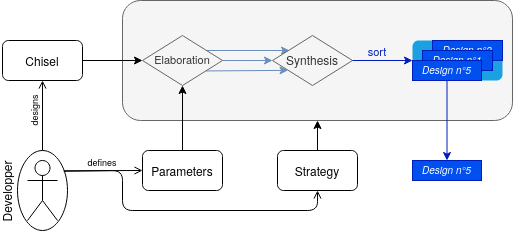
\includegraphics[width=0.85\textwidth]{Figures/DSE-exhaustive}
                \caption{Simple exhaustive strategy\vspace{0.3cm}}
                \label{ch.dse:sec.functional:ssec.complex:fig.complex:sfig.exhaustive}
            \end{subfigure}
            \begin{subfigure}{1.0\textwidth}
                \myAlignmentSpace
                %1.32
                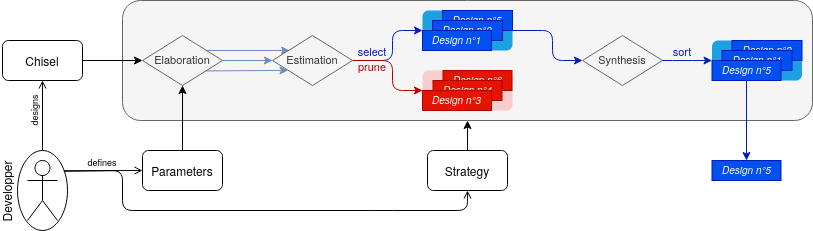
\includegraphics[width=1.36\textwidth]{Figures/DSE-pruning}
                \caption{Pruning based strategy\vspace{0.3cm}}
                \label{ch.dse:sec.functional:ssec.complex:fig.complex:sfig.pruning}
            \end{subfigure}
            \begin{subfigure}{1.0\textwidth}
                \myAlignmentSpace
                %1.19
                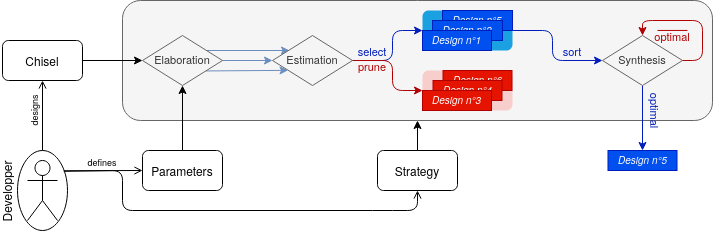
\includegraphics[width=1.23\textwidth]{Figures/DSE-gradient}
                \caption{Gradient descent based strategy}
                \label{ch.dse:sec.functional:ssec.complex:fig.complex:sfig.gradient}
            \end{subfigure}
            \caption{Building complex strategies}
            \label{ch.dse:sec.functional:ssec.complex:fig.complex}
        \end{figure}


%%%%%%%%%%%%%%%%%%%%%%%%%%%%%%%%%%%%%%%%%%%%%%%%%%%%%%%%%%%%%%%%%%%%%%%%%%%%%%%%%

\clearpage
\section[Discussions on the Proposed DSE Methodology]{Discussions on the Proposed Design Space Exploration Methodology}
\label{ch.dse:sec.discussion}
    \subsection{Limitations of the Approach}
    \label{ch.dse:sec.discussion:ssec.limitations}

        Our approach strongly relies on the quality of the estimators to perform quick space traversals while achieving accurate estimations, with the objective to provide realistic solutions.

        It is even more true when looking at the proposed frequency estimation methodology, as it remains as complex as what synthesis is --- in an algorithmic meaning --- and will probably not cope with the \myLongAcs{FPGA}{Field-Programmable Gate Array} specificities, resulting in erroneous estimations after potentially longer processes.
        However, more accurate estimation methods exist at various levels of granularity which could improve the explorations quality, and our methodology would greatly benefit from proposing to its users both multi-level and multi-fidelity estimators \cite{ye_scalehls_2021}\cite{lo_multi-fidelity_2018}.

        On the other hand, more complex exploration schemes are yet to be proposed in order to achieve state of the art exploration performances, notably by using meta heuristics for \myLongAc{MOP}{Multi-objective Optimization Problem} solving (such as \myLongAcs{GA}{Genetic Algorithm} \cite{paletti_dovado_2021}, Bayesian optimization \cite{lo_model-based_2016} or simulated annealing \cite{witschen_circa_2019}), or supervised learning techniques \cite{nardi_practical_2019}\cite{ferretti_leveraging_2020}.

        The proposed schemes are here introduced as a {\it proof of concept} of functional programming usage for efficient \myAc{DSE}, and the introduced library of basic strategies should be enhanced.

    \subsection{Synthesis on the Contributions}
    \label{ch.dse:sec.discussion:ssec.synthesis}

        Using the estimation considerations that were exposed in Chapter \ref{ch.estimators}, as well as the \myLongAcs{HCL}{Hardware Construction Language} features, we defined two complementary methodologies for \myLongAc{DSE}{Design Space Exploration} --- namely {\bf meta design} and {\bf meta exploration}.

        We put a particular focus on how functional programming can be used to define exploration strategies, by leveraging users expertise to build exploration processes step by step.
        We then exposed various basic schemes that can be used to build both application and target specific strategies.

        The proposed methodologies are built considering naive use cases, and both new estimation methodologies and exploration strategies should be proposed in order to provide a more flexible approach.
        

%%%%%%%%%%%%%%%%%%%%%%%%%%%%%%%%%%%%%%%%%%%%%%%%%%%%%%%%%%%%%%%%%%%%%%%%%%%%%%%%%
%%%%%%%%%%%%%%%%%%%%%%%%%%%%%%%%%%%%%%%%%%%%%%%%%%%%%%%%%%%%%%%%%%%%%%%%%%%%%%%

\cleardoublepage
%-------------------------------------------------------------------------------
\chapter{Experiments and Results}
\labelchapter{ch.expe}
%-------------------------------------------------------------------------------

%%%%%%%%%%%%%%%%%%%%%%%%%%%%%%%%%%%%%%%%%%%%%%%%%%%%%%%%%%%%%%%%%%%%%%%%%%%%%%%%
%%%%%%%%%%%%%%%%%%%%%%%%%%%%%%%%%%%%%%%%%%%%%%%%%%%%%%%%%%%%%%%%%%%%%%%%%%%%%%%%

\lettrine[lines=2]{T}{his} chapter introduces the experiments that were run to demonstrate the usability of both the estimation and the exploration methodologies that were described in the previous chapters.

We built a \chisel-based demonstrator as a {\it proof of concept} framework, as well as a benchmark of representative applications for analysis and comparison purposes.
We then ran multiple experiments to exhibit how \myLongAcs{HCL}{Hardware Construction Language} can be used to improve the life of developers, with a particular focus on their usage for \myLongAc{DSE}{Design Space Exploration}.

\vspace*{\fill}
\minitoc 
\mtcskip 

\newpage
%%%%%%%%%%%%%%%%%%%%%%%%%%%%%%%%%%%%%%%%%%%%%%%%%%%%%%%%%%%%%%%%%%%%%%%%%%%%%%%%

% SECTION
\section{Building a Software Demonstrator}
\label{ch.expe:sec.qece}
    In order to demonstrate the usability of the methodologies introduced in Sections \ref{ch.estimators} and \ref{ch.dse}, we built a \chisel-based framework --- which is called \myLongAc{QECE}{Quick Exploration using Chisel Estimators} --- and integrated it into the \myLongAc{HCF}{Hardware Construction Framework}.

    \subsection{Implementation Details}
    \label{ch.expe:sec.qece:ssec.impl}

        \myAc{QECE} was built in a flexible and modular way, to allow users to easily define both custom estimators and exploration strategies.
        It leverages \scala{} high level features to use software methodologies in hardware design processes.
        
        \subsubsection{Meta design}
            To do so, the first step was to enable users to exploit the {\bf meta design methodology}, in order to expose the design space to be explored at module constructor level, as stated in Section \ref{ch.dse:sec.explorable:ssec.generators}.
            This was made possible by using the \java{} annotation system (as can be seen in Listing \ref{ch.dse:sec.explorable:ssec.generators:list.dotproduct} for example).
            We also added an annotation system to specify the impact of the parameters on given metrics, enabling to leverage the user knowledge at both implementation and exploration stages, by introducing a relationship between parameters and strategies.
            It is done by defining a new annotation class: \lstinline{class ImpactMetric(name: String) extends StaticAnnotation} --- where the \lstinline{name} parameter is used to identify a particular metric.\footnote{The \lstinline{@qualityOfService} annotation used in Listing \ref{ch.dse:sec.explorable:ssec.generators:list.dotproduct} is a simple alias for \lstinline{ImpactMetric("qualityOfService")}.}

        \subsubsection{Integrating estimators}
            In a second time, we developed wrappers around the \firrtl{} transforms to enable a seamless estimator integration, as exposed in Section \ref{ch.estimators:sec.integration:ssec.api}.

            We implemented both {\bf resource} and {\bf timing} estimators using linear interpolations and macro block replacements to allow an early estimation of the metrics in the exploration flows.

            Some empirical \myLongAc{QoS}{Quality of Service} estimators were implemented by binding to the \chisel{} simulation backends, as shown in Figure \ref{ch.estimators:sec.integration:ssec.multi-fidelity:fig.flow}.
            Doing so, one can retrieve some metrics from simulations, and can thus build their own test benches, defining both which metrics they want to get and how they are computed.
            As an example, we added helpers to compute the \myLongAcs{RMSE}{Root-Mean-Square Error} from the simulation results, by providing an initial workload and a software golden reference.

            Finally, we enabled building any {\bf analytical estimator} operating on pre-existing metrics in the flow --- users can thus easily define analytical formulas directly in their strategies.

        \subsubsection{Building strategies}
            We then built a flexible way to enable {\bf meta exploration} by implementing a generic \lstinline{Strategy} class, which can then be used to define more or less complex strategies, as defined in Section \ref{ch.dse:sec.functional}.

            \begin{figure}[h!]
                \centering
                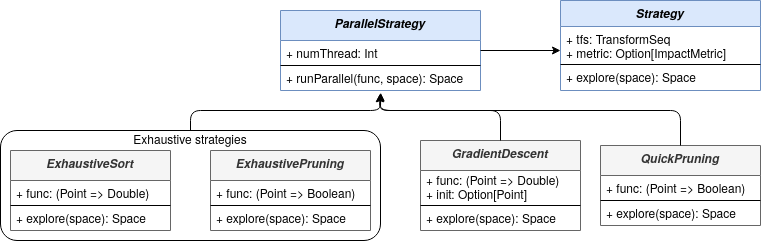
\includegraphics[width=1.0\textwidth]{Figures/Implementation-Strategies.png}
                \caption{Object hierarchy for the implemented strategies}
                \label{ch.expe:sec.qece:ssec.impl:fig.strategies}
            \end{figure}

            Figure \ref{ch.expe:sec.qece:ssec.impl:fig.strategies} introduces the different strategies that were built for this demonstrator, which have already been discussed in Section \ref{ch.dse:sec.functional:ssec.basic}.
            As we can see, every implemented strategy inherits from the base \lstinline{Strategy} class through \lstinline{ParallelStrategy}, as each can take advantage of parallel threads to speed-up the estimations.
            The strategies rely on custom defined parameters that allow the users to finely tune every step of the process --- it includes the {\bf estimation transforms} \lstinline{tfs} to be run, the {\bf number of parallel threads} available, or different ways to estimate and compare the explored implementations. 
            For both {\bf pruning strategies}, the users hence need to provide a {\bf boolean function} which specify if a point should be removed from the space, while the two other strategies rely on a {\bf cost function} which build a new metric from a set of existing ones.

            The \lstinline{ImpactMetrics} are considered at strategy level to reduce the design space dimension by removing the non impacting parameters if needed.
            The same mechanism is used for the dimension removal strategy that was exposed in Section \ref{ch.dse:sec.functional:ssec.basic}, in order to allow users to explicitly state that a given dimension will no more be relevant for the remaining of an exploration process.
            Moreover, as the introduced estimation processes are independent, we also implemented some helpers for parallelism exploitation in order to speed up the whole processes --- this is particularly helpful for time consuming estimation processes such as synthesis runs --- and we used caching techniques in the strategies to avoid multiple estimations of a same point. 
            We finally implemented composition and strategy building helpers as a syntactic sugar to enable straightforward strategy definitions in a functional fashion --- \ie the helpers hide all the side-effects needed for the strategy building, and expose the exploration processes as simple functions operating over spaces.

        \vspace{-0.15cm}
        \subsubsection{Design space implementation}
        \vspace{-0.05cm}
            Building custom exploration strategies is thus made possible in a expressive way.
            However, implementing a new strategy often relies on particular operations over the input space, implying that the data structure used for its implementation might have a huge impact on the exploration performances.

            In order to allow the users to define their own space structures, we propose a generic implementation for \lstinline{Spaces} in Figure \ref{ch.expe:sec.qece:ssec.impl:fig.space}, with the basic operations introduced in Section \ref{ch.dse:sec.functional} that are needed to explore them (\eg \lstinline{map}, \lstinline{filter} or \lstinline{getNeighbours} functions).
            It also includes operations to remove and add dimensions, for cases where the \lstinline{ImpactMetric}s are used to discriminate some dimensions in the current exploration.
            We use a hierarchical, object-oriented approach to allow the users to easily integrate their own space structures if needed.
            As each implementation defines its own operations, some spaces might be more suited for a given usage, and the strategy builder should choose a structure fitted for their need.
            For the needs of this demonstrator, we implemented two different structures: \lstinline{SeqSpaces} and \lstinline{MatrixSpaces}.

            A \lstinline{SeqSpace} is a simple space based on the \scala{} \lstinline{Seq} collections, that can be used for sort purposes as it exposes an ordered structure.
            However, finding the neighbourhood of a multidimensional \lstinline{Point} in a flatten representation of the space requires to scan it exhaustively, evaluating each distance and selecting only the nearest points.
            As a \lstinline{SeqSpace} does not exhibit any pattern to directly access to the neighbourhoods, exploring the neighbours of a \lstinline{Point} in a large space can thus result in an exploding complexity.

            On the other hand, a \lstinline{MatrixSpace} is based on the \scala{} representation of matrices, built on multidimensional \lstinline{Arrays}. 
            Each dimension of the space is represented at a different level in the built {\bf hyper matrix}, and the space also includes a dictionary mapping each dimension to all the possible values.
            This enables to easily define the neighbourhood of a point, with a complexity growing linear with the different dimensions of the space (which is ideal to define efficient {\bf gradient descent based strategies}).
            This also means that the matrices may be sparse, for points that have already been pruned.
            However, such \lstinline{Space} cannot be sorted as the structure does not exhibit an order, and the \scala{} \lstinline{Array}-based implementations can only be used for dimensions ranging from 1 to 5 --- which is a limitation of the language --- even if adding dimensions is possible in a custom way if needed.

\clearpage
            \begin{figure}[h!]
                \centering
                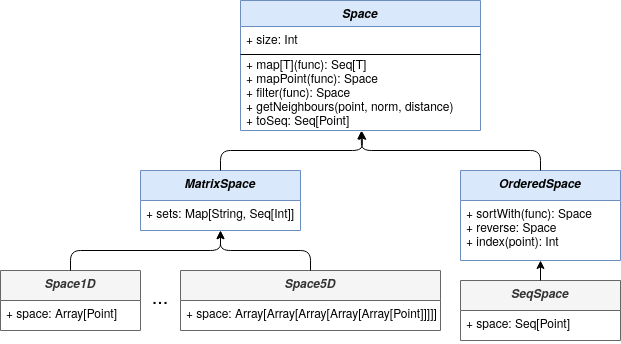
\includegraphics[width=1.0\textwidth]{Figures/Implementation-Space.png}
                \caption{Proposing different space implementations}
                \label{ch.expe:sec.qece:ssec.impl:fig.space}
            \end{figure}

        \subsubsection{A functional demonstrator}
            Using those two space implementations and the five basic strategies introduced in Chapter \ref{ch.dse}, we built \myAc{QECE} as a {\it proof of concept} framework that will be used to demonstrate the advantages of the proposed methodologies.

            We deliver \myAc{QECE} as an open-source solution, to enable using the introduced methodologies in any \chisel-based project \cite{ferres_qece_2021}.

    \subsection{Use Case: Exploring GEMM Implementations}
    \label{ch.expe:sec.qece:ssec.usecase}

            We introduce a (simplified) example of the usage of \myAc{QECE} for a {\bf gradient descent based exploration} on \myLongAc{GEMM}{General Matrix Multiply} kernels in Listing \ref{ch.expe:sec.qece:list.gradient}, implementing the strategy exposed in Figure \ref{ch.dse:sec.functional:ssec.complex:fig.complex:sfig.gradient}.

            For each strategy, the user needs to define the set of {\bf estimation transforms} \lstinline{tfs} to be run, and some functions to specify the exploration behaviour:%
            \footnote{ The \lstinline{++} operation is used to build an ordered set of {\bf estimation transforms}.} %
            for both \lstinline{sort} and \lstinline{gradient} steps, he needs to provide a function \lstinline{func} to associate a cost to each implementation, as well as a comparison function \lstinline{cmp} to expose an order relationship, while the \lstinline{prune} step only requires a boolean function (also called \lstinline{func}) to specify whether a point is to be removed or to be kept in the resulting design space.

            The different metrics at stake in this use case are \lstinline{%lut}, \lstinline{%dsp} and \lstinline{throughput}, which respectively corresponds to the usage of \myAcs{LUT} and \myAcs{DSP}, and to the theoretical throughput of the considered implementations.

            The defined strategy is based on three consecutive steps:
            \begin{enumerate}
                \item {\bf lines 2-5:} Estimate the resource usages and {\bf prune the implementations} that consume {\bf too many resources}.\footnote{Thresholds are arbitrary and shall depend on the accuracy of the used estimators.}
                \item {\bf lines 7-10:} Sort the design space to {\bf select the widest implementation} that still fits on the target board, after this first pruning.
                \item {\bf lines 12-17:} Use this implementation as the starting point of a {\bf gradient descent algorithm} based on synthesis runs, aiming to find local optimum in an already pruned space (using the {\bf throughput (GOp/s)} as the objective function to optimize).
            \end{enumerate}

            As the \myAc{GEMM} algorithm is computation intensive, we chose to consider only the \myLongAcs{LUT}{Look-Up Table} and \myLongAcs{DSP}{Digital Signal Processor} usages for step 1., as the wide implementations will probably saturate the available \myAcs{LUT}/\myAcs{DSP} before the other resources --- it is important to note that this decision is based on our expertise about hardware design.
            For step 2., we then chose to define the {\bf widest design} as the implementation estimated to consume the greatest amount of \myAcs{LUT} for similar reasons, with the hypothesis that the implementation with the maximal throughput --- but that still fits on the target board --- will be near this estimated widest implementation.
            This is then used in step 3., as the gradient strategy will use the first point of the sorted space as the starting point for the descent.
            We thus improve the convergence speed as we know that the implementations where both \myAcs{LUT} and \myAcs{DSP} are estimated to be low will probably not be the optimal ones.

            We defined some aliases for the estimation transforms to be run, to keep the strategy concise and intelligible:
            \begin{itemize}
                \item \lstinline{TransformSeq.resources} performs a \firrtl{} estimation of the circuit resource usage, using the methodology introduced in Section \ref{ch.estimators:sec.resource-timing}.
                \item \lstinline{TransformSeq.synthesis} runs a synthesis backend and performs a report analysis to provide both resource usage and operating frequency.
                \item \lstinline{TransformSeq.throughput} computes the throughput using an analytical formula (Eq. \ref{app.benchmark:sec.gemm:eq.throughput}).
                    The implementations that did not fit on the target board after the synthesis are marked as having a null throughput.
            \end{itemize}

\clearpage
            Using those transforms, we can express the exploration flow schematized in Figure \ref{ch.dse:sec.functional:ssec.complex:fig.complex:sfig.gradient} in a readable, intelligible manner, by composing exploration steps in a functional fashion.
            Each exploration step --- \ie \lstinline{prune}, \lstinline{sort} and \lstinline{gradient} --- corresponds to a \lstinline{Strategy} as defined in Section \ref{ch.expe:sec.qece:ssec.impl}, defining the estimation transforms to be run and the \lstinline{Space} operations to be performed, resulting in a complex, application specific strategy.


        \begin{figure}[h!]
            \begin{lstlisting}[caption={[Gradient based strategy definition]Defining a gradient descent based strategy (Fig. \ref{ch.dse:sec.functional:ssec.complex:fig.complex:sfig.gradient}) in QECE},
                               label={ch.expe:sec.qece:list.gradient}]
explore(
    // prune the designs using too much DSP/LUT
    prune(
        tfs  = TransformSeq.resources,
        func = (%dsp > x || %lut > y)
    ),
    // select the widest design to start descent
    sort(
        func = %lut,
        cmp  = (\_ > \_)
    ),
    // use gradient descent for exploration
    gradient(
        tfs  = TransformSeq.synthesis ++ 
               TransformSeq.throughput,
        func  = throughput,
        cmp   = (\_ > \_)
    )
)\end{lstlisting}
        \end{figure}

%%%%%%%%%%%%%%%%%%%%%%%%%%%%%%%%%%%%%%%%%%%%%%%%%%%%%%%%%%%%%%%%%%%%%%%%%%%%%%%%%

% SECTION
\section{Application Benchmark}
\label{ch.expe:sec.benchmark}

    To demonstrate how \myAc{QECE} can be used to improve the developer productivity, we built an open-source benchmark of digital applications that are relevant for \myAc{FPGA}-based implementations \cite{ferres_benchmark_2021}.

    Appendix \ref{app.benchmark} exposes how the {\bf meta design} methodology has been applied to each kernel of the benchmark.
    More specifically, Table \ref{app.benchmark:table.benchmark} introduces its composition as well as all the exposed design spaces.
    
%%%%%%%%%%%%%%%%%%%%%%%%%%%%%%%%%%%%%%%%%%%%%%%%%%%%%%%%%%%%%%%%%%%%%%%%%%%%%%%%%

% SECTION
\section{Experimental Setups}
\label{ch.expe:sec.setup}

    The experiments were run on two different experimental setups, as two servers were available.
    Their characteristics are introduced in Table \ref{ch.expe:sec.setup:table.setup}.

    \begin{table}[h!]
        \centering
        \begin{tabular}{cccccc}
            {\bf Name} & {\bf Mark} & {\bf\#Core} & {\bf Frequency} & {\bf RAM} & {\bf Vivado} \\
            \hline
            Server 1 & \pomahaka & 12 & 3.46 GHz & 78.8 GB & v2017.3\\
            \ccg Server 2 & \ccg\styx & \ccg 24 & \ccg 3.2 GHz & \ccg 188 GB & \ccg v2021.1\\
        \end{tabular}
        \caption{Experimental setups characteristics}
        \label{ch.expe:sec.setup:table.setup}
        \vspace{-0.4cm}
    \end{table}

    It is important to note that \vivado{} specifications claims that at most {\bf 8 GB} of \myAc{RAM} will be used when targeting a \VC{} board \cite{xilinx_memory_2021}.
    % It is important to note that \vivado{} memory usage specifications claims that at most {\bf 8 GB} will be used when targeting a \VC{} board \cite{xilinx_memory_2021}.
    However, the memory consumption is given only for designs that consume $\approx 80\%$ of the available resources --- meaning that, for wider designs, the memory usage may explode.
    To cope with this problem, we had to define a {\bf 2-hours synthesis timeout}, in order to keep the memory usage under constraint and avoid crashes.
    We empirically noticed that doing so keeps the memory usage under 20 GB for each synthesis, meaning that we can respectively run at most 4 and 9 synthesis at once on server 1 and 2.
    As the version of \vivado{} can lead to different implementation choices, it is important to consider which version of the software suite was used for syntheses --- it is also important to note that given the version and/or the synthesis heuristics used, synthesis results may vary a lot: the whole flow is highly dependent on the quality of the synthesis software used.

    For the next sections, please refer to the column {\bf Mark} to know which setup was used for a particular experiment.

%%%%%%%%%%%%%%%%%%%%%%%%%%%%%%%%%%%%%%%%%%%%%%%%%%%%%%%%%%%%%%%%%%%%%%%%%%%%%%%%%

% SECTION
\section{Quality of the Estimators}
\label{ch.expe:sec.estimators}

    In this section, we will discuss the quality of the estimation methodologies that were defined in Chapter \ref{ch.estimators}, and show that our demonstrator is able to leverage imperfect yet exploitable estimators for both resource and \myAc{QoS} metrics.
    We will also tackle the usability of our approach for timing estimation, as well as limitations of such approach in quick exploration processes.

    \subsection{Resource Estimations}
    \label{ch.expe:sec.estimators:ssec.resource}

        Figure \ref{ch.expe:sec.estimators:ssec.resource:fig.all} introduces a measure of the \myLongAc{QoR}{Quality of Results} of the {\bf graph level resource estimators} --- or \firrtl-based estimators --- that were described in Section \ref{ch.estimators:sec.resource-timing}.
        The \myAc{QoR} is computed with respect to the synthesis results for 5 different {\bf meta designs} (see Table \ref{ch.expe:sec.estimators:ssec.resource:table.kernels}).

        For each implementation, we ran three types of resource estimators:%
        \footnote{To keep both resource usage and processing time acceptable, we set a {\bf 30 minute timeout} for both macro replacement and resource usage estimation transforms.}
        \begin{enumerate}
            \setlength\itemsep{-.3em}
            \item \firrtl-based estimation, without macro block (see Section \ref{ch.estimators:sec.resource-timing:ssec.basic})
            \item \firrtl-based estimation, using macro blocks (see Section \ref{ch.estimators:sec.resource-timing:ssec.macro})
            \item {\bf Synthesis} based estimation, used as baseline (\ie reference value)
        \end{enumerate}

        We then plotted the relative difference histograms of both estimations 1. and 2. with respect to 3., respectively in Figures \ref{ch.expe:sec.estimators:ssec.resource:fig.all:sfig.without} and \ref{ch.expe:sec.estimators:ssec.resource:fig.all:sfig.with}, to analyse the \myAc{QoR} of both estimation methodologies.
        To do so, for each implementation of each kernel, we tried to run those three estimators, computed the relative differences with respect to the synthesis results, and built relative difference classes for each resource type (\myAcs{LUT}, \myAcs{FF}, \myAcs{DSP} and \myAcs{BRAM}).
        Those classes were then plotted in order to exhibit the impact of each estimation methodology, for all the considered resources.
        
        \begin{figure}[h!]
            \vspace{-0.2cm}
            \centering
            \begin{subfigure}{1.0\textwidth}
                \centering
                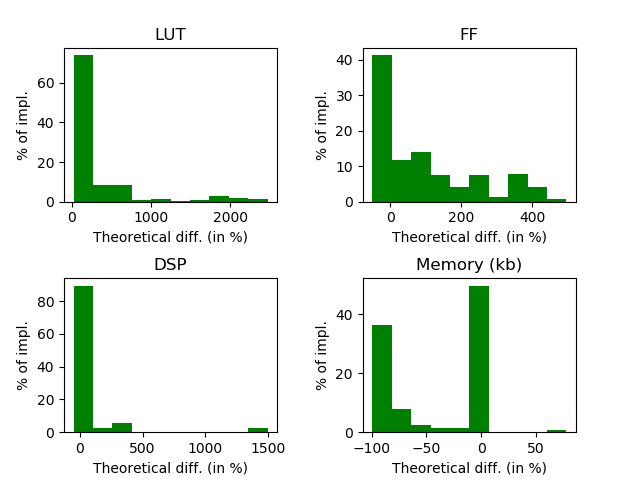
\includegraphics[width=0.83\textwidth]{Figures/results/allRelativeWithoutMacro}
                \caption{Resource estimation (without macro block replacement)}
                \label{ch.expe:sec.estimators:ssec.resource:fig.all:sfig.without}
            \end{subfigure}
            \begin{subfigure}{1.0\textwidth}
                \centering
                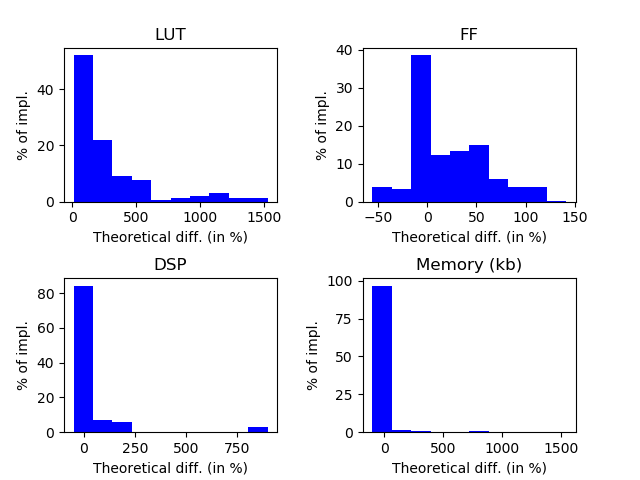
\includegraphics[width=0.83\textwidth]{Figures/results/allRelativeWithMacro}
                \caption{Resource estimation (with macro block replacement)}
                \label{ch.expe:sec.estimators:ssec.resource:fig.all:sfig.with}
            \end{subfigure}
            \caption[Quality of resource estimations on various kernels]{Average relative differences on 5 different {\bf meta designs} between the resource estimations and the synthesis results.\textsuperscript{\styx}\newline The kernels are introduced in Table \ref{ch.expe:sec.estimators:ssec.resource:table.kernels}.}
            \label{ch.expe:sec.estimators:ssec.resource:fig.all}
        \end{figure}

        \renewcommand*{\thefootnote}{\fnsymbol{footnote}}
        \begin{table}[h!]
            \scalebox{0.9}{
                \begin{tabular}{cccccc}
                    \multirow{2}*{{\bf Kernel}} & \multirow{2}*{{\bf Space}} & {\bf Estimations} & \multicolumn{3}{c}{{\bf Estimation time}} \\
                    ~ & ~ & {\bf ({\it failures})} & Synthesis &  Macro & No macro\\
                    \hline
                    \myAc{GEMM}\footnotemark[9] & 168 & 151 (46) & 15h48m11s & 2h00m42s & 25m55s \\
                    \ccg Black Scholes\footnotemark[9] & \ccg 162 & \ccg 42 (3) & \ccg 2h57m16s & \ccg 10m19s & \ccg 8m12s \\
                    Pi\footnotemark[9] & 162 & 90 (12) & 39m50s & 4m14s & 1m05s \\
                    \ccg \myAc{FFT}\footnotemark[9] & \ccg 200 & \ccg 173 (22) & \ccg 9h51m16s & \ccg 3h14m06s & \ccg 2h14m37s\\
                    Dot product\footnotemark[9] & 144 & 144 (0) & 27m54s & 29s & 26s \\
                    \hline
                    \hline
                    {\bf Total} & {\bf 836} & {\bf 600 (83)} & {\bf 29h44m27s} & {\bf 5h59m50s} & {\bf 2h50m15s}\\
                \end{tabular}
            }
            \caption[Temporal behaviour of resource estimators]{Design spaces and running times of resource estimators (Fig. \ref{ch.expe:sec.estimators:ssec.resource:fig.all})}
            \label{ch.expe:sec.estimators:ssec.resource:table.kernels}
        \end{table}
        \renewcommand*{\thefootnote}{\arabic{footnote}}

        We observe that using the naive approach --- \ie without macro block replacement (Fig. \ref{ch.expe:sec.estimators:ssec.resource:fig.all:sfig.without}) --- the estimation accuracy is quite variable:
        \begin{itemize}
            \item the \myAcs{LUT} are estimated within $[\![0\%, 1000\%]\!]$ of the real usage for more than 80\% of the considered designs
            \item the \myAcs{FF} are estimated within $[\![0\%, 400\%]\!]$ of the real usage, and even under 200\% for a majority of designs
            \item the \myAcs{DSP} are almost always estimated perfectly, but errors in the estimations may result in a 1500\% overestimation
            \item the \myAcs{BRAM} are estimated within $[\![-100\%, 100\%]\!]$ of the real usage, and are perfectly estimated for a majority of designs
        \end{itemize}

\clearpage
        Based on the Figure \ref{ch.expe:sec.estimators:ssec.resource:fig.all:sfig.with}, we can then remark that using macro block replacements has a big impact on the estimations \myAc{QoR}.
        The \myAc{LUT} estimations are now mainly produced in a $[\![0\%, 500\%]\!]$ interval, while the \myAc{FF} estimations are now estimated within $[\![-50\%, 100\%]$.
        The \myAc{DSP} estimations are mainly as good as with the naive version, but extrema are divided by a factor 2, and the \myAc{BRAM} usage is now always perfectly estimated.

        We can thus claim that those estimators are not perfect, and that the estimation variability could be considered too big to be exploitable.
        However, some tendencies can be exhibited here, that could be used to take decisions based on the estimations only:
        \begin{itemize}
            \item for most designs, using a factor 6 on the \myAc{LUT} estimation can enable to estimate whether a design fits on the target board or not
            \item similarly, using a factor 2 for \myAcs{FF} can lead to realistic decisions
            \item both \myAc{DSP} and \myAc{BRAM} estimations can be trusted for most designs
        \end{itemize}

        As for the estimation process speed, we can observe in Table \ref{ch.expe:sec.estimators:ssec.resource:table.kernels} that both the naive and the macro based approaches are way faster than synthesis runs, which was the main objective of those techniques.
        We can also remark that using the macro block replacement methodology can consume a lot more time that the naive approach, and it is specifically true for large and complex designs such as \myAc{GEMM} or \myAc{FFT}.
        It is actually due to the implementation of the macro replacement technique, which is based on building another graph from the \myAc{FIRRTL} representation, and which does not seem to scale on large designs.
        Most of the time is due to timeouts of the graph building processes, and this could be mitigated by using a more optimized technique to do so.

        We thus showed that the graph level techniques that were introduced in Chapter \ref{ch.estimators} can be used to perform an early resource estimation, and could be leveraged for early decision making from the developers.        
        However, we still need to exhibit what impact it can have on those decisions, and it will be discussed later in this chapter.

        \subsubsection*{Remark}
        While we did exhibit the \myAc{QoR} of the estimation methodologies on 5 different {\bf meta designs}, one may want to analyse the quality of both methodologies for a particular kernel. 
        For this purpose, we expose a disaggregated version of Figure \ref{ch.expe:sec.estimators:ssec.resource:fig.all} in Appendix \ref{app.resource} --- except for the \myAc{GEMM} kernels, which results are exposed in Figure \ref{ch.expe:sec.strategies:ssec.resource:fig.gemm} as they will be used in later experiments.

    \subsection{Timing Estimations}
    \label{ch.expe:sec.estimators:ssec.timing}

       As for the timing estimations, Figure \ref{ch.expe:sec.strategies:ssec.timing:fig.gemm} introduces some considerations on both the estimation processing times and the \myAc{QoR} for \myAc{GEMM} kernels, with respect to the synthesis results.
       Table \ref{ch.expe:sec.estimators:ssec.timing:table.gemm} provides more information about the explored design space and the temporal behaviour of these experiments.%
       \footnote{For the naive approach --- \ie without macro block replacement --- the timing estimations are not fully available, as the memory blocks cannot properly be estimated.
       However, the path building algorithm was run anyway to estimate the processing time.}

        \begin{table}[h!]
            \scalebox{0.9}{
                \begin{tabular}{c|cccc}
                    \multirow{2}*{{\bf Space size}} & \multirow{2}*{{\bf Estimator}} & {\bf Successful} & \multirow{2}*{{\bf Timeouts}} & \multirow{2}*{{\bf Exploration time}} \\ 
                    ~ & ~ & {\bf estimations} & ~ & ~ \\
                    \hline
                    \multirow{5}*{168} & Synthesis & 102 & 49 & 15h48m24s\\
                    ~ & \ccg RTL estimation & \ccg ~ & \ccg ~ & \ccg ~\\
                    ~ & \ccg (with macro) & \multirow{-2}*{\ccg 94} & \multirow{-2}*{\ccg 57} & \multirow{-2}*{\ccg 11h20m15s}\\
                    ~ & {\it RTL estimation} & ~ & ~ & ~\\
                    ~ & {\it (without macro)} & \multirow{-2}*{-} & \multirow{-2}*{-} & \multirow{-2}*{{\it $\approx$8h}}\\
                \end{tabular}
            }
            \caption[Timing estimations over GEMM implementations]{Timing estimations over GEMM\textsuperscript{\styx} implementations (Fig. \ref{ch.expe:sec.strategies:ssec.timing:fig.gemm})}
            \label{ch.expe:sec.estimators:ssec.timing:table.gemm}
        \end{table}

       For those experiments, a {\bf 2 hours timeout} was used for both macro replacement and critical path estimation transforms, in order to keep the memory usage under constraints and avoid time consuming processes.
       Doing so, we remark that for both timing estimation approaches --- \ie with and without macro block replacement --- the estimation time is mostly kept way under the synthesis time.
       However, for complex designs, it can be longer than the synthesis.
       This is mainly due to the complexity of the path building algorithm, which unrolls every possible path on the considered design, and is thus similar to the synthesis process --- hence, it cannot be considered as a faster approach, as the algorithmic complexities are comparable.

        \begin{figure}[h!]
            \centering
            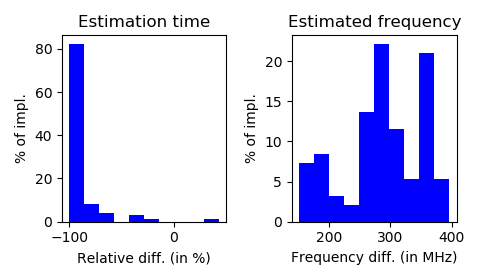
\includegraphics[width=1.0\textwidth]{Figures/results/gemmTimingWithMacro}
            \caption[Quality of frequency estimations on GEMM]{Relative difference between frequency estimations and synthesis\newline results on GEMM {\bf meta design}\textsuperscript{\styx} ({\it using macro block replacement})}
            \label{ch.expe:sec.strategies:ssec.timing:fig.gemm}
        \end{figure}

       Using only those considerations, we can already state that those approaches cannot be leveraged to build efficient design processes, as for more complex designs, actually synthesizing the circuit will result in a faster feedback for the users.
       Moreover, we can also remark that the frequency estimation is totally unrealistic, with differences of hundred of MHz between the estimations and the synthesis results.
        
       Based on those results, we consider this timing estimation methodology to be unpracticable with both approaches, and will not consider those estimators to be usable in the rest of this work.
       However, some methods exist to provide more realistic estimations of the operating frequency \cite{kwon_transfer_2020}\cite{paletti_dovado_2021}, and integrating them in \myAc{QECE} is considered, as they could bring both fast and interesting feedbacks to users and tools.

    \subsection{Quality of Service Estimations}
    \label{ch.expe:sec.estimators:ssec.qos}

        In order to estimate the \myAc{QoS} of a design, we propose an \myLongAc{API}{Application Programming Interface} to users in order to extract custom defined results from a simulation backend, as specified in Section \ref{ch.expe:sec.qece:ssec.impl}.
        To define an estimator, one needs to provide a {\bf simulation test bench} as well as a way to compute and extract the \myAc{QoS} of the design with respect to a given workload.% providing a generic way to define any empirical metric.

        Figure \ref{ch.expe:sec.estimators:ssec.qos:fig.qos} introduces a simple use case on the {\bf dot product} kernel, using \myAc{RMSE} as an error metric.
        We here provide a simple analysis of the impact of the data representation on the result of a dot product, and display the error rate, showing that integrating a custom defined \myAc{QoS} metric is possible in \myAc{QECE}.
        To define the data representation, we use a fixed point format and consider two parameters: the number of bits used for the {\it dynamic} (\ie the number of bits before the binary point), and the number of {\it precision} bits (\ie after the binary point).
        As the {\it parallelism level} does not impact the \myAc{QoS}, this dimension is not considered, while the number of elements by input vector is fixed to 8, for visualization purposes.

\clearpage
        \begin{figure}[h!]
            \centering
            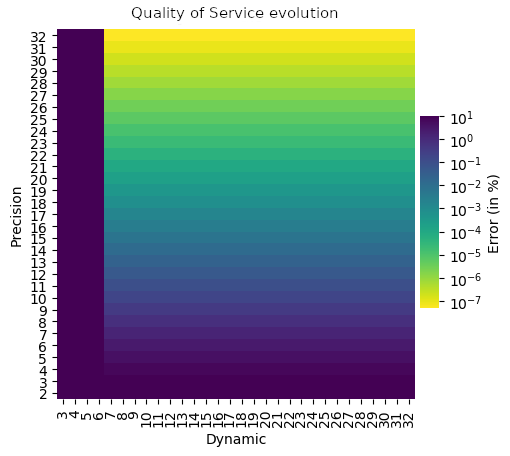
\includegraphics[width=1.0\textwidth]{Figures/results/qosEstimation.png}
            \caption[Quality of Service estimations on dot product]{Heatmap of the Quality of Service estimations for the dot\newline product {\bf meta design}\textsuperscript{\styx} ({\it vector size is fixed to 8 elements})}
            \label{ch.expe:sec.estimators:ssec.qos:fig.qos}
        \end{figure}

        The empirical approach for this estimator is based on comparing the simulation results with a software version of the same algorithm, based on a floating-point representation.
        Doing so, we can select only the designs which do not introduce a significant error in their results --- on this use case, it actually enables to compare the different data representations to select the ones sufficiently wide to absorb the errors that are induced by the use of a simpler representation.
        As the hardware implementation of \myLongAcs{FPU}{Floating-Point Unit} requires a lot of resources and time, such approach can be used to select a more efficient way to implement an algorithm, if the users can precisely state which error rates are acceptable.

\clearpage
        As can be seen on the heatmap, the implementations that use not enough {\it dynamic} bits are marked with a 10\% error rate, as representation overflows occurred during the simulations, resulting in a large error.%
        \footnote{The error rate introduced in Fig. \ref{ch.expe:sec.estimators:ssec.qos:fig.qos} is capped at 10\% and uses a logarithmic scale to properly visualize the smaller error rates, which are the region of interests in such explorations, as the acceptable error rate should be under 10\% to be meaningful.}
        Moreover, we can also observe the impact of the {\it precision} parameter on the \myAc{QoS}, from large representations where the error rate is under $10^{-7}\%$ to more compact ones, where the error rate reaches 10\%.

        While this use case is quite simple, it demonstrates that one can easily integrate an empirical, application specific estimator to estimate the \myAc{QoS} of its circuits, providing him with an interesting feedback that can be leveraged to select the best implementation that satisfy its accuracy need.

        For example, in Figure \ref{ch.expe:sec.estimators:ssec.qos:fig.qos}, we can (visually) state that if the applicative needs require an error rate lesser than 0.1\%, any implementation with more than 6 bits of {\it dynamic} and 10 bits of {\it precision} is enough.
    
%%%%%%%%%%%%%%%%%%%%%%%%%%%%%%%%%%%%%%%%%%%%%%%%%%%%%%%%%%%%%%%%%%%%%%%%%%%%%%%%%

\section{Comparing the Exploration Strategies}
\label{ch.expe:sec.strategies}
    We will now discuss how the user expertise can be leveraged for an efficient \myAc{DSE} definition, using the methodologies introduced in Chapter \ref{ch.dse}.

    For each strategy that will be compared in this section, the strategy definition is based on assumptions on both considered algorithm and target board, as our approach is based on providing users with ways to exploit their expertise instead of trying to define generic strategies for every algorithm.

    \subsection{Resource Estimation and Convergence Speed}
    \label{ch.expe:sec.strategies:ssec.resource}
    
        In a first time, we want to demonstrate how high level estimations of the resource usage can be used for the quicker convergence of an exploration strategy.
        We consider the exploration of two different {\bf meta designs} --- \myAc{FFT} and \myAc{GEMM} --- and compare the three exploration strategies that were introduced in Figure \ref{ch.dse:sec.functional:ssec.complex:fig.complex}.
        The results are exposed in Table \ref{ch.expe:sec.strategies:ssec.resources:table.explo}.
        For those experiments, the \myAc{QoS} is not considered, hence the element width is fixed by the developer (assuming that they can specify at exploration time that the chosen data representation is acceptable for the given use case), meaning that the {\it bit width} dimension is not considered in those explorations.

\clearpage
        \begin{table}[ht!]
            \centering
            \scalebox{0.68}{
                \centering
                \begin{tabular}{|c|c|c|c|c|c|c|c|}
                    \hline
                    \multirow{2}*{\bf Kernel} & \multirow{2}*{\bf Strategy} & \multirow{2}*{\bf Best throughput} & \multirow{2}*{\bf \#(space)} & {\bf \#synth} & \multirow{2}*{\bf Time} & \multirow{2}*{\bf Speed-up} \\
                    ~ & ~ & ~ & ~ & (\#timeout) & ~ & ~ \\
                    \hline
                    \multirow{3}*{\myAc{FFT}128\textsuperscript{\pomahaka}} & {\it Exhaustive} (Fig. \ref{ch.dse:sec.functional:ssec.complex:fig.complex:sfig.exhaustive}) & {\it 1.767 Tb/s} & \multirow{3}*{7} & {\it 7 (0)} & {\it 00h22m45s} & - \\
                    ~ & Pruning (Fig. \ref{ch.dse:sec.functional:ssec.complex:fig.complex:sfig.pruning}) & 1.767 Tb/s & ~ & 7 (0) & 00h24m14s & \inred{$\times$0.94} \\
                    ~ & Gradient (Fig. \ref{ch.dse:sec.functional:ssec.complex:fig.complex:sfig.gradient}) & 1.767 Tb/s & ~ & 3 (0) & 00h19m51s & $\times$1.15 \\
                    \hline
                    \multirow{3}*{\myAc{FFT}512\textsuperscript{\pomahaka}} & {\it Exhaustive} & {\it 5.479 Tb/s} & \multirow{3}*{9} & {\it 9 (0)} & {\it 02h11m51s} & - \\
                    ~ & Pruning & 5.479 Tb/s & ~ & 9 (0) & 03h17m52s & \inred{$\times$0.66} \\
                    ~ & Gradient & 5.479 Tb/s & ~ & 3 (0) & 02h18m29s & \inred{$\times$0.95} \\
                    \hline
                    \multirow{3}*{\myAc{GEMM}\textsuperscript{\pomahaka}} & {\it Exhaustive} & {\it 231.334 GOp/s} & \multirow{3}*{41} & {\it 41 (19)} & {\it 13h51m56s} & - \\
                    ~ & Pruning &  231.334 GOp/s & ~ & 26 (7) & 08h52m00s & $\times$1.5 \\
                    ~ & Gradient & 231.334 GOp/s & ~ & 6 (1) & 03h21m06s & $\times$4.1 \\
                    \hline
                \end{tabular}
                }
                \caption[Strategy comparison with no QoS concerns]{Comparing different exploration strategies with no quality of service concerns. {\it (Exhaustive strategies are used as baselines)}}
                \label{ch.expe:sec.strategies:ssec.resources:table.explo}
        \end{table}
\vspace{-0.6cm}
        \subsubsection{Defining a pruning function}

            For both kernels, we used a simple hypothesis to define the pruning function:
            \hyp{ch.expe:sec.strategies:ssec.resources:hyp.pruning}{Both FFT and GEMM kernels are computation intensive.}
            This means that the computational resources --- \ie \myAcs{LUT} and \myAcs{DSP} --- will be saturated first by the synthesis tool, and that removing too wide designs can be done by considering only those metrics.

            We thus defined the following {\bf pruning function} to be applied in both {\bf pruning} and {\bf gradient} strategies:
            \begin{equation}
                \label{ch.expe:sec.strategies:ssec.resource:eq.pruning}
                prune_{est.}(p) = LUT_{est.}(p) > 200\% \vee DSP_{est.}(p) > 100\%
            \end{equation}
            The thresholds were chosen with respect to the considerations that were discussed in Section \ref{ch.expe:sec.estimators:ssec.resource} and to the \myAc{QoR} of the resource estimations on \myAc{GEMM} kernels, as presented in Figure \ref{ch.expe:sec.strategies:ssec.resource:fig.gemm:sfig.with}.

            \subsubsection{Exploring {\it Fast Fourier Transform} implementations}

                For the \myAc{FFT} explorations, the design spaces are reduced as the size of the algorithm (see Table \ref{app.benchmark:table.benchmark} for the instantiation parameters) is considered fixed by the developers at exploration time --- meaning that \myAc{FFT} implementations of different sizes are not compared during the exploration processes.
                This results in a single dimension exploration space to be explored, for each possible \myAc{FFT} size.
                We only considered two different sizes --- 128 and 512 --- and we remark that for both explorations, the {\bf pruning strategy} is slower than the baseline, as no actual pruning is done in the design space.
                In fact, we actually applied the exhaustive strategy after running resource estimations, resulting in a consequent overhead with respect to the baseline.

                On the other hand, we remark that the {\bf gradient strategy} results in less synthesis needs for the same best fit finding --- meaning that even if the exploration time is not much impacted by the strategy choice, we can reduce the global processor time needed for parallel syntheses.
                In fact, for the \myAc{FFT}512, the actual convergence time is biased by synthesis timeouts, meaning that improving the resource estimators could enable to prune more efficiently the design space, and could help us avoiding long and non converging syntheses.% in the process.

                These use cases can be used to discuss the importance of the adequacy between the chosen exploration strategy and the explored kernel.
                Indeed, applying a preliminary pruning function to those use cases is not useful to speed-up explorations, and just results in a useless time overhead, while the gradient approach is practical and results in a speed-up that compensates that overhead.

            \subsubsection{Exploring {\it General Matrix Multiply} implementations}

            \begin{figure}[h!]
            \centering
            \begin{subfigure}{1.0\textwidth}
                \centering
                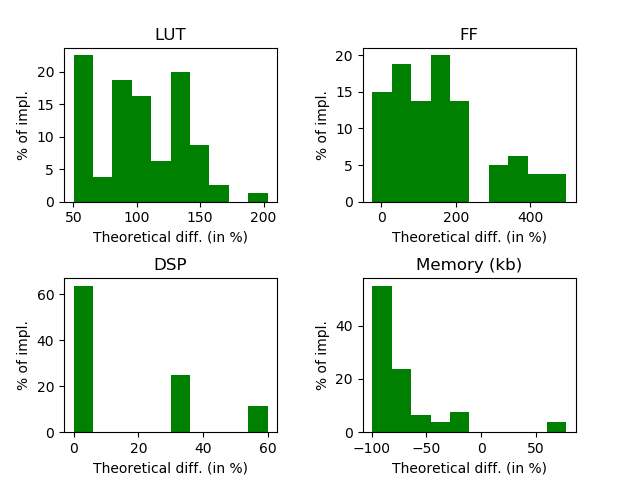
\includegraphics[width=0.85\textwidth]{Figures/results/gemmRelativeWithoutMacro}
                \caption{Resource estimation (without macro block replacement)}
                \label{ch.expe:sec.strategies:ssec.resource:fig.gemm:sfig.without}
            \end{subfigure}
            \begin{subfigure}{1.0\textwidth}
                \centering
                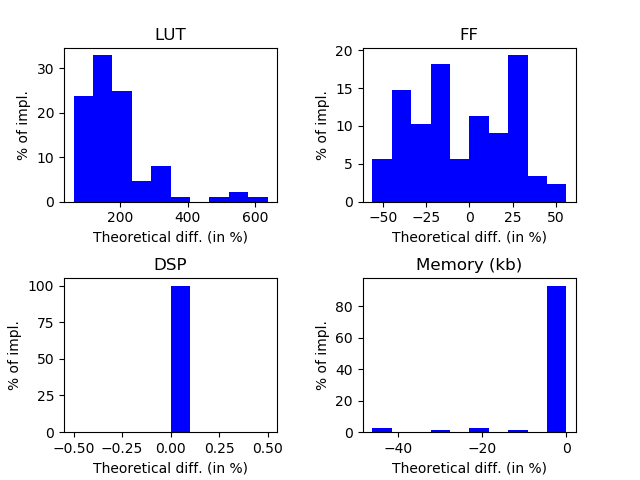
\includegraphics[width=0.85\textwidth]{Figures/results/gemmRelativeWithMacro}
                \caption{Resource estimation (with macro block replacement)}
                \label{ch.expe:sec.strategies:ssec.resource:fig.gemm:sfig.with}
            \end{subfigure}
            \caption[Quality of resource estimations on GEMM]{Relative difference between resource estimations and synthesis\newline results on GEMM implementations\textsuperscript{\styx}}
            \label{ch.expe:sec.strategies:ssec.resource:fig.gemm}
        \end{figure}

                For the \myAc{GEMM}-based explorations, we assumed that the defined pruning function (Eq. \ref{ch.expe:sec.strategies:ssec.resource:eq.pruning}) is more relevant, as it is based on an analysis of the \myAc{QoR} of the estimators on the \myAc{GEMM} implementations.
                We observe that applying this pruning function enables to reduce the number of implementations to be synthesized in the {\bf pruning strategy} by more than a third.
                More importantly, it reduces the number of synthesis timeouts by more than a half, as some non fitting designs that would cause long or non converging synthesis processes are not considered in this approach.

                In addition to this, we observe that using the {\bf gradient strategy} --- \ie leveraging both high level resource estimations and clever space traversal --- results in $\times 6.8$ less synthesis runs (6 instead of 41) and a $\times 4.1$ exploration speed-up.

                We thus showed that building an application specific, user defined strategy enables to speed-up exploration processes while producing comparable solutions for this use case.

                \subsubsection{Disclaimer on the definition of the pruning function}
                    One could argue that defining the pruning function after synthesizing the whole design space to analyse the \myAc{QoR} of the resource estimators is not practical, as the goal of this methodology is to avoid such exhaustive exploration.
                    This is mainly due to the fact that the applied estimation methodology is application specific --- as the {\bf meta designs} characteristics have a heavy impact on the resource estimator \myAc{QoR} (see Appendix \ref{app.resource} for more information) --- and could be addressed by providing more accurate and reliable resource estimators in the framework.
                    This could be used to define more generic pruning thresholds that would not require to run application specific syntheses to define it.
                    We could also run syntheses on a subset of the target design space to define this pruning function.% --- in fact, both \myAc{LUT} and \myAc{DSP} threshold could have been estimated without running exhaustive synthesis over the design space.

    \subsection{Quality of Service Based Explorations}
    \label{ch.expe:sec.strategies:ssec.qos}

        We now consider the \myAc{QoS} of the generated designs, and demonstrate how the proposed methodologies can enable to define multi-concern exploration strategies for custom \myLongAc{MOP}{Multi-objective Optimization Problem} solving.
        In contrast to the previous explorations, we do not make any assumption over the data representation --- particularly over the bit widths --- and delegate the responsibility of choosing a relevant data type to the exploration flow.

        \subsubsection{Comparing different pruning strategies}

            To begin with, we analyse the impact of the pruning strategies over both quality and speed of the pruning.
            In other words, we will compare the {\bf exhaustive} and the {\bf quick pruning} strategies defined in Section \ref{ch.dse:sec.functional:ssec.basic} to check that the {\bf quick pruning} strategy prunes the same implementations that the exhaustive approach does, while exhibiting the impact of the implementation details on the run time.

            First of all, we use the {\bf dot product meta design} to measure the \myAc{QoS} of each implementation using empirical transforms.
            To select only the implementations that are compliant with the accuracy needs, the user provides an {\bf error threshold} --- here accepting a 1\% error rate --- and uses the provided heuristic for {\bf quick pruning} (Fig. \ref{ch.expe:sec.strategies:ssec.qos:fig.quick}) to partition the different spaces more efficiently than by applying an exhaustive filtering.
            The heatmap represents the results of the exhaustive approach to illustrate the distribution of the error rates, while the grey squares constitute the frontier that was built in the Algo. \ref{ch.dse:sec.functional:ssec.basic:algo.quick}, and is used to build the pruned design space in the end (\ie the implementations that are "above" the frontier).
            We remark that both strategies produce the same resulting space, meaning that the {\bf quick pruning strategy} can be used for quicker convergence of \myAc{QoS}-based explorations, at least for kernels that are assumed to comply with Hypothesis \ref{ch.dse:sec.functional:ssec.basic:hyp.quick}.


\clearpage
            \begin{figure}[h!]
                \centering
                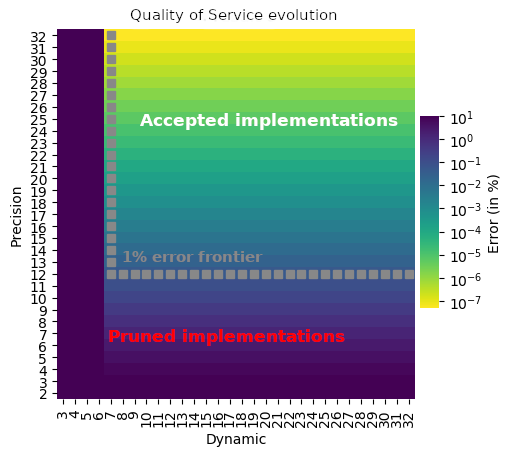
\includegraphics[width=1.0\textwidth]{Figures/results/quickPruning_annotated.png}
                \caption[Quick pruning of design space]{Quick pruning strategy for Quality of Service based exploration on\newline the dot product {\bf meta design}\textsuperscript{\styx} ({\it considering vectors of 8 elements})}
                \label{ch.expe:sec.strategies:ssec.qos:fig.quick}
            \end{figure}
        
            \begin{table}[ht!]
                \centering
                \begin{tabular}{cccc}
                    {\bf Optimization} & {\bf Simulated impl.} & {\bf Time} & {\bf Speed-up}\\
                    \hline
                    {\it Exhaustive pruning} & {\it 3844} & {\it 12m22s} & {\it ---}\\
                    \ccg Space reduction + & \ccg ~ & \ccg ~ & \ccg ~\\
                    \ccg exhaustive pruning & \ccg \multirow{-2}*{961} & \ccg \multirow{-2}*{03m07s} & \ccg \multirow{-2}*{$\times 3.97$}\\
                    Space reduction + & \multirow{2}*{255} & \multirow{2}*{05m03s} & \multirow{2}*{$\times 2.44$}\\
                    quick pruning (SeqSpace) & ~ & ~ & ~\\
                    \ccg Space reduction + & \ccg ~ & \ccg ~ & \ccg ~\\
                    \ccg quick pruning (MatrixSpace) & \ccg \multirow{-2}*{255} & \ccg \multirow{-2}*{00m49s} & \ccg \multirow{-2}*{$\times 15.14$}\\
                \end{tabular}
                \caption[Pruning results with respect to used optimizations]{Pruning results with respect to the used optimization on\newline the dot product {\bf meta design}\textsuperscript{\styx}}
                \label{ch.expe:sec.strategies:ssec.qos:table.quick}
            \end{table}

\clearpage
            We now consider the impact of both strategies and of the implementation details on the runtime.
            Table \ref{ch.expe:sec.strategies:ssec.qos:table.quick} exposes 4 different ways to prune the design space, that are based on the composition of three techniques:
            \begin{itemize}
                \item Space reduction --- \ie reducing the number of explored dimensions using the users knowledge about the parameters impact (Section \ref{ch.dse:sec.explorable:ssec.space})
                \item Strategy choice --- either the exhaustive or the quick pruning strategy% (Algo. \ref{ch.dse:sec.functional:ssec.basic:algo.quick})
                \item Space structure choice ---  either using a \lstinline{SeqSpace} or a \lstinline{MatrixSpace}
            \end{itemize}

            For all the considered techniques, we empirically checked that the resulting design spaces are identical, meaning that the same pruning is performed by those 4 techniques.
            The impact of the space reduction technique on the exploration time is obviously linear, as the number of estimated implementations is reduced in a linear way.
            In this context, as the {\it parallelism} parameter is not considered for \myAc{QoS}-based explorations, we reduce by a $\times 4$ factor the number of considered implementations (as this parameter can take 4 different values).
            Moreover, the number of implementations to simulate (column {\bf Simulated impl.} is also impacted by the chosen exploration strategy, as using the {\bf quick pruning} heuristic can lead to a relevant partition with less simulations to run, with respect to the {\bf exhaustive pruning} strategy.

            We can also remark that the performance of the {\bf quick pruning strategy} heavily relies on the chosen space structure: using a \lstinline{SeqSpace} representation, the quick pruning is actually slower than the exhaustive strategy, while using a \lstinline{MatrixSpace} results in a $\times 3.8$ $(= 15.14 / 3.97)$ speed-up, with respect to the strategy using both exhausting pruning and space reduction.

            We thus showed on this simple example that the {\bf quick pruning strategy} can be used to speed-up a \myAc{QoS}-based exploration strategy.
            Moreover, we provide further analysis about the \myAc{QoS} estimation and the quick pruning strategy in Appendix \ref{app.quick}.

\clearpage
        \subsection{Use Case: Exploring Black Scholes Designs}
        \label{ch.expe:sec.strategies:ssec.bs}
            We now consider a more realistic use case to demonstrate how the proposed methodologies can be leveraged to build a complex, application specific exploration strategy.
            To do so, we use a {\bf Black Scholes meta design} --- for which the implementation details are provided in Appendix \ref{app.benchmark} --- and define an iterative exploration strategy based on our expertise of \myAc{FPGA} design.

            As exposed in Appendix \ref{app.benchmark}, the {\bf meta design} exposes 5 parameters: the data representation parameters (\ie {\it dynamic} and {\it precision}), the number of iterations of the {\bf Monte Carlo} method, the number of parallel cores available, and the number of iterations of the {\bf Euler-Maruyama} method.

            \subsubsection{Defining the objectives of the exploration}
                The first thing to do to define an efficient exploration process is to clearly state the goal of the target flow.
                In this {\bf Black Scholes} based use case, we decided to try to \textbf{\emph{maximize the throughput of the generated accelerators, under the constraints that they fit on the target board and produce results with a controlled error rate}}.

                \begin{equation}
                    \label{ch.expe:sec.strategies:ssec.bs:eq.throughput}
                    T_{estimation.s^{-1}} = \frac{freq}{\Delta_c}
                \end{equation}

                \begin{equation}
                    \label{ch.expe:sec.strategies:ssec.bs:eq.latency}
                    \Delta_c \approx \frac{nbIter \times nbEuler}{nbCore}
                \end{equation}

                The throughput --- expressed in number of estimations by second --- can be approximated easily for these kernels, as they periodically produce a result: it is then computed as the ratio between the {\bf frequency} and the {\bf latency} of a given implementation (Eq. \ref{ch.expe:sec.strategies:ssec.bs:eq.throughput}).
                A theoretical latency (in number of cycles) --- \ie the (fixed) period between the production of each result --- can be computed using the Equation \ref{ch.expe:sec.strategies:ssec.bs:eq.latency}, as a huge majority of the computation cycles are spent in the {\bf Monte Carlo} cores iterations.%
                \footnote{This result has been verified empirically, proving that the impact of the control flow variations on the latency is negligible with respect to the actual computation cycles.}

                We also define an {\bf area} metric to verify that a design fits on the target board, using the maximum values of the usage percentage for the four considered metrics (\myAcs{LUT}, \myAcs{FF}, \myAcs{DSP} and \myAcs{BRAM}). 

            \subsubsection{Enhancing the design space}
                The next step to take in the introduced methodology is to instrument the {\bf meta design} with information on the metrics that will be used in the flow.

                \begin{figure}[ht!]
                    \begin{lstlisting}[xleftmargin=0mm,
                                       caption={[Expertise-based design space for Black Scholes meta design]Expertise-based design space for Black Scholes {\bf meta design}},
                                       label={ch.expe:sec.strategies:ssec.bs:list.bsSpace}]
class BlackScholes(
    @resource @qos @linear(8, 32)  dynamic: Int,
    @resource @qos @linear(8, 32)  precision: Int,
    @qos @pow2(5, 10)              nbIteration: Int,
    @qos @pow2(1, 6)               nbEuler: Int,
    @resource @pow2(2, 10)         nbCore: Int
) extends Module with Explorable\end{lstlisting}
                \vspace{-0.4cm}
                \end{figure}

                For this exploration, we will sequentially consider two concerns: a first stage will be based on the circuits \myAc{QoS}, and a second one will work over their resource usage.
                We hence need to define, for both of those metrics, which parameters have an impact on them, and which does not, based on our knowledge about the algorithm.
                The analysis to do so is introduced below, and is used to enhance the initial design space as exposed in Table \ref{app.benchmark:table.benchmark}, leading to the one introduced in Listing \ref{ch.expe:sec.strategies:ssec.bs:list.bsSpace}.

                Due to the probabilistic nature of the {\bf Monte Carlo} method, most of the exposed parameters have an impact on the \myAc{QoS}, either because they act on the data representation (as it is the case for both {\it precision} and {\it dynamic} parameters), or because they impact the number and the precision of the sampling in the Black Scholes equation (Eq. \ref{app.benchmark:sec.monteCarlo:eq.bsem}), as do the {\it number of iterations} and the {\it number of Euler-Maruyama iterations}.
                In contrast with these statements, the {\it number of cores} does not impact the circuits \myAc{QoS}, as it only modifies the temporal behaviour of the designs, and not their functionalities --- this parameter is hence not annotated as impacting the quality of service (using the \lstinline{@qos} annotation).

                As for the resource usage, we now try to identify which parameters impact the size of the generated designs.
                We can use our knowledge about the meta design structure to state that both {\it iteration parameters} (the global number of {\bf Monte Carlo} iterations, and the number of inner {\bf Euler-Maruyama} iterations) does not significantly impact the amount of resources used in a design.
                As a matter of fact, the number of iterations will act on the global latency of the design (Eq. \ref{ch.expe:sec.strategies:ssec.bs:eq.latency}), but will have a small impact on the resource usage, which mostly depends on the number of parallel cores and their size.%
                \footnote{The number of iterations actually impacts some counters in the control flow of the designs --- however, the impact is negligible with respect to the resources needed to implement the computation cores.}
                We thus annotate the data representation parameters and the {\it nbCore} parameter with \lstinline{@resource} to guide the exploration steps.

\clearpage
\vspace{-0.5cm}
            \subsubsection{Outlining the estimation transforms}
                Once the design space has been enhanced to guide the exploration, we need to define the different steps that are to be taken in the process.
                To build a compact definition of this exploration strategy, we define some helpers in Listings \ref{ch.expe:sec.strategies:ssec.bs:list.simu} and \ref{ch.expe:sec.strategies:ssec.bs:list.transforms} to build the transforms that are to be used in the flow.

                Listing \ref{ch.expe:sec.strategies:ssec.bs:list.simu} demonstrates how empirical \myAc{QoS} estimators can be integrated in \myAc{QECE}, in a condensed way.
                We define \lstinline{QualityOfService.simulation} as a transform calling the simulation backend to estimate the \myAc{RMSE} of a given implementation.
                The different {\bf generation parameters} of the simulated implementation are needed to instantiate the simulation test bench, and are thus retrieved from the {\bf point metrics} (the \lstinline{m} variable at line 1., which is used to define the parameters in lines 5-9).
                Moreover, some other parameters can be provided by the users when they are building such {\bf estimation transform} --- \eg in this use case, they provide the number of software iterations (line 10.) to compute the reference value for the {\bf Black Scholes} estimation, as well as the number of hardware simulations to run on each implementation to provide a significant result (line 11.).
                They also provide a {\it workload} (line 12.), which is the data distribution to be used in the test benches.

                \underline{Remark:} The circuits \myAc{QoS} are estimated using an empirical approach (Section \ref{ch.estimators:seq.qos:ssec.empirical}), as we use it to demonstrate the practicability of using the simulation backend in the estimation methodologies.
                However, one could also define an analytical formula to specify the relationship between the number of iterations of a given implementation on one hand, and the accuracy of the {\bf Black Scholes} approximation on the other.
                 While it would not be used to estimate the impact of the data representation over the \myAc{QoS}, it could allow to eliminate the parameters relative to the number of iterations from the design space, at least for the exploration steps that rely on simulations.

                As for Listing \ref{ch.expe:sec.strategies:ssec.bs:list.transforms}, it implements the analytical formulas from Equations \ref{ch.expe:sec.strategies:ssec.bs:eq.throughput} and \ref{ch.expe:sec.strategies:ssec.bs:eq.latency}.
                The transforms are easily defined, by specifying a pair $(n \rightarrow f: \{m_x, x \in [\![0, p]\!]\} \Rightarrow m_{x_{p+1}})$ with $n$ the name of the generated metric, and $f$ a function which operates on a set of metrics $\{m_x, x \in [\![0, p]\!]\}$ to generate a new metric named $n$ to be propagated in the exploration process.

                As can be seen in lines 1-4, the {\bf latency} is estimated in the {\bf pre-elaboration} stage (with respect to the \myAc{API} introduced in Section \ref{ch.estimators:sec.integration:ssec.api}), as it only relies on the generation parameters.

                On the other hand, both {\bf area} and {\bf throughput} are estimated in the {\bf post-elaboration} stage (lines 5-12).
                This is due to the fact that the \lstinline{Transforms.throughput} method is going to be called in the same exploration step that the synthesis flow:  as the formulas rely on the synthesis results, they must be computed after the elaboration process.

\clearpage
                The \lstinline{area} metric is computed by retrieving each resource percentage metric from the current implementation, using the maximal value to check if a design fits on the target board.
                To artificially eliminate the non fitting designs, we then use a temporary metric \lstinline{_throughput} to store the theoretical throughput as computed using Equation \ref{ch.expe:sec.strategies:ssec.bs:eq.throughput} (lines 8-9), but only assign it to the actual \lstinline{throughput} metric if the \lstinline{area} metric is under 100\% (lines 10-11).

\vspace{-0.4cm}
                \begin{figure}[h!]
                    \begin{lstlisting}[xleftmargin=0mm,
                                       basewidth={0.55em, 0.5em},
                                       caption={Defining an helper for empirical quality of service estimations},
                                       label={ch.expe:sec.strategies:ssec.bs:list.simu}]
object QualityOfService {
  val simulation = TransformSeq.simulation(m =>
    (                                                                       
      c =>                                                                                                        
        new BlackScholesTester(                                                                                   
          m("dynamic").toInt,                                                                                     
          m("precision").toInt,                                                                                   
          m("nbIteration").toInt,                                                                                 
          m("nbCore").toInt,                                                                                      
          m("nEuler").toInt,                                                         
          nbSoftIteration,                                                                                             
          nbSimulation,                                                                                                 
          workload                                                                                                
        )(c)                                                                                                      
      )                                                                                                           
    )                                                                                                            
}\end{lstlisting}
                \end{figure}
\vspace{-1.1cm}
                \begin{figure}[h!]
                    \begin{lstlisting}[xleftmargin=0mm,
                                       basewidth={0.55em,0.5em},
                                       caption={Transform helper for the exploration},
                                       label={ch.expe:sec.strategies:ssec.bs:list.transforms}]
object Transforms {
  val latency = TransformSeq.preElab(
    "latency" ->
      (m => (m("nbIteration") * m("nbEuler")) / m("nbCore"))
  )
  val throughput = TransformSeq.postElab(
    "area" ->
      (m => max(m("lut"), m("ff"), m("dsp"), m("mem"))),
    "_throughput" ->
      (m => m("freq") / m("latency")),
    "throughput" ->
      (m => if (m("area") > 1.0) 0.0 else m("_throughput"))
  )
}\end{lstlisting}
                \end{figure}

\clearpage
            \subsubsection{Defining the exploration strategy}
                After defining the transforms that are going to be used in the exploration process, the last step is to define the steps to be taken.
                We define a {\bf five steps} strategy for this use case, for which the code is exposed in Listing \ref{ch.expe:sec.strategies:ssec.bs:list.strategy}:
                \begin{enumerate}
                    \item \underline{\bf lines 1-5:} the design space is pruned for implementations that are estimated to induce an error of more than {\bf 5\%} (line 3.).

                        For this step, we use the {\bf quick pruning} algorithm (Algo. \ref{ch.dse:sec.functional:ssec.basic:algo.quick}) to quickly partition the space in this pruning step (line 1.).
                        Moreover, as we only consider the \myAc{QoS} of the different implementations, we specify that the framework can eliminate all the dimensions that are not annotated with \lstinline{@qos} (line 4.).
                        Indeed, we use the \lstinline{QualityOfService.simulation} transform from Listing \ref{ch.expe:sec.strategies:ssec.bs:list.simu} to compute the \myAc{QoS} (line 2.).
                    \item \underline{\bf line 6:} this line specifies how we reduce the dimensions of the design space for the remaining exploration steps.
                        All the {\bf meta design parameters} (see Fig. \ref{ch.expe:sec.strategies:ssec.bs:list.bsSpace}) that are not annotated with \lstinline{@resource} do no act on the resource metrics, and are thus removed from the dimensions. 
                        They are in fact the parameters acting on the number of iterations: {\it nbIteration} and {\it nbEuler}.
                        Actually, we can state two things at this point: all the remaining designs are acceptable with respect to the needed \myAc{QoS} in this use case, and reducing the number of iterations can only benefit to improve both the resource usage and the throughput.%
                        \footnote{Increasing the number of iterations can only improve the \myAc{QoS} at the cost of {\bf latency} increase (Eq. \ref{ch.expe:sec.strategies:ssec.bs:eq.latency}), yet we already have a sufficiently low error after the pruning step.}

                        The boolean parameter of the \lstinline{context.reduceDimension} method specifies that the dimension removal will project the parameters on the {\bf minimal values} in the space --- as we want to keep the number of iterations as low as possible among the remaining designs.

                        By removing those two dimensions from the design space, the number of remaining implementations is hence heavily reduced.%, which allows to speed-up the process.
                    \item \underline{\bf line 7:} we compute the latency of each remaining implementation.
                    \item \underline{\bf lines 8-12:} we select the "minimal point" of the remaining design space (the point with the minimal sum of parameters) and put it in front of the design space, as the next step will use it as a starting point.
                    \item \underline{\bf lines 13-17:} we use a {\bf gradient descent} algorithm to find a local optimum with respect to the objective of the exploration.

                        In this step, we run syntheses in order to provide a realistic estimation of both resource usage and operating frequency, and it is thus necessary to adopt a clever strategy to limit the number of costly process runs.
                        We hence use neighbourhood explorations to iteratively find an acceptable solution to the users.
                \end{enumerate}

                \begin{figure}[h!]
                    \begin{lstlisting}[xleftmargin=0mm,
                                       basewidth={0.55em, 0.5em},
                                       caption={[Black Scholes exploration strategy]Expertise-based exploration strategy for Black Scholes\newline implementations},
                                       label={ch.expe:sec.strategies:ssec.bs:list.strategy}]
val strategy = context.buildStrategy(                                                                                    
  context.quickPrune[BlackScholes](                                                                             
    QualityOfService.simulation,
    _.error > 0.05,                                                                                            
    metric = Some(new qos)                                                                              
  ),                                                                                                                
  context.reduceDimension[BlackScholes](new resource, true),                                                    
  context.map[BlackScholes](Transforms.latency),                                                     
  context.sort[BlackScholes](                                                                                   
    TransformSeq.empty,                                                                                           
    m => m("dynamic") + m("precision") + m("nbCore"),                                                                 
    (_ < _)                                                                                                           
  ),                                                                                                                  
  context.gradient[BlackScholes](                                                                               
    TransformSeq.synthesis ++ Transforms.throughput
    func = _("throughput"),                                                                                           
    cmp = (_ > _)  
  )                                    
)\end{lstlisting}
                \end{figure}

                We hence defined a complex, expertise-based exploration strategy which takes the best of the users knowledge to guide the framework and to speed-up the traversal process.
                In order to provide an analysis on the relevance of such strategies, we ran multiple exploration processes to expose the interests of the {\bf meta exploration} choices that led to the definition of Listing \ref{ch.expe:sec.strategies:ssec.bs:list.strategy}.
                
        \subsection{Results of the Black Scholes Exploration}
        \label{ch.expe:sec.strategies:ssec.results}
            In this last section, we will analyse the results of the exploration strategy defined for the Black Scholes use case, to exhibit the advantages of defining a custom strategy in a functional fashion.

\clearpage
            \subsubsection{Comparing the pruning strategies}
                A first analysis can be done about the quality of the pruning processes, by comparing the {\bf exhaustive pruning} and the {\bf quick pruning} strategies on the Black Scholes use case.

                % \tdf{quality of service pruning + venn fiagramm}
                \begin{table}[ht!]
                    \begin{tabular}{ccccc}
                        {\bf Error} & {\bf Number} & \multirow{2}*{{\bf Strategy}} & {\bf Exploration} & \multirow{2}*{{\bf Speed-up}} \\
                        {\bf threshold} & {\bf of impl.} & ~ & {\bf time} & ~ \\
                        \hline
                        \ccg ~ & \ccg ~ & \ccg Exhaustive pruning & \ccg 46h29m19s & \ccg - \\
                        \multirow{-2}*{\ccg 5\%} & \multirow{-2}*{\ccg 202500} & \ccg Quick pruning & \ccg 32h59m29s & \ccg $\times 1.40$ \\
                        \multirow{2}*{2\%} & \multirow{2}*{202500} & Exhaustive pruning & 46h21m42s & - \\
                        ~ & ~ & Quick pruning & 48h46m53s & \inred{$\times 0.95$}
                    \end{tabular}
                    \caption[Comparing pruning strategies on Black Scholes]{Comparing the pruning strategies over Black Scholes kernels\textsuperscript{\styx}}
                    \label{ch.expe:sec.strategies:ssec.bs:table.qor}
                \end{table}

                \begin{figure}[h!]
                    % \centering
                    \begin{subfigure}{0.49\textwidth}
                        \centering
                        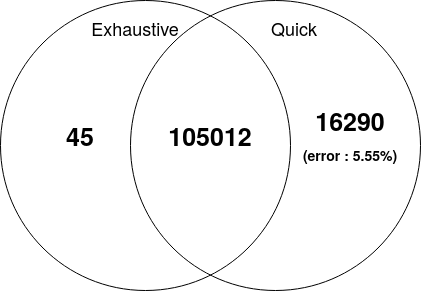
\includegraphics[width=1.0\textwidth]{Figures/results/qor-venn-5}
                        \caption{5\% error threshold}
                        \label{ch.expe:sec.strategies:ssec.bs:fig.venn:sfig.5}
                    \end{subfigure}
                    ~
                    \begin{subfigure}{0.49\textwidth}
                        \centering
                        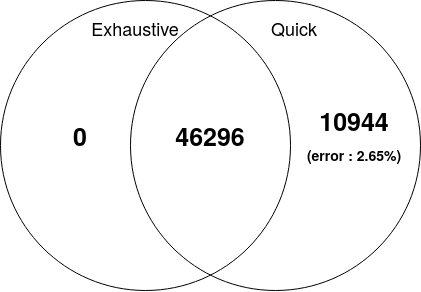
\includegraphics[width=1.0\textwidth]{Figures/results/qor-venn-2}
                        \caption{2\% error threshold}
                        \label{ch.expe:sec.strategies:ssec.bs:fig.venn:sfig.2}
                    \end{subfigure}
                    \caption[Comparing the accuracy of the pruning strategies]{Comparing the accuracy of the pruning strategies on Black Scholes\textsuperscript{\styx}}
                    \label{ch.expe:sec.strategies:ssec.bs:fig.venn}
                \end{figure}

                Table \ref{ch.expe:sec.strategies:ssec.bs:table.qor} introduces the results of four different explorations processes, to compare both strategies using two different {\bf error thresholds} for the pruning.
                In those experiments, only the pruning step (lines 1-5 in Listing \ref{ch.expe:sec.strategies:ssec.bs:list.strategy}, compared to an exhaustive version of it) is considered, and we compare the remaining implementations in Figure \ref{ch.expe:sec.strategies:ssec.bs:fig.venn}.

                As we can see in the table, depending on the error threshold, the {\bf quick pruning strategy} can lead to a faster pruning of the space (as it is the case with a 5\% threshold), or a slower one if the frontier is difficult to estimate and requires a lot of neighbourhood exploration steps to do so.

                We can also see in Figure \ref{ch.expe:sec.strategies:ssec.bs:fig.venn} that the quick pruning heuristic is not perfect: %
                for example, using an acceptable error rate of 5\% (Fig. \ref{ch.expe:sec.strategies:ssec.bs:fig.venn:sfig.5}), {\bf 105012 remaining implementations} were common to both strategies, while {\bf 45} were pruned by the quick strategy and not by the exhaustive one, and {\bf 16290} were pruned by the exhaustive strategy, and not by the quick one (on a total of {\bf 202500 different implementations}).
                If we consider the exhaustive pruning to be the baseline --- as estimating the \myAc{QoS} of each implementation leads to a more realistic pruning of the design space, even if the empirical approach can induce erroneous data --- we can remark that the quick pruning strategy tends to prune less implementations that the exhaustive one.

                This shows that this strategy can lead to erroneous choice from the exploration tools --- however, the average errors in the designs that should have been pruned by the quick heuristic but were not are also displayed in Figures \ref{ch.expe:sec.strategies:ssec.bs:fig.venn:sfig.5} and \ref{ch.expe:sec.strategies:ssec.bs:fig.venn:sfig.2} (with average errors of respectively 5.55\% and 2.65\%).
                These errors are computed on the points that were estimated in the frontier building algorithms, through the neighbourhood exploration: those implementations are thus near to this limit, and this is why they are not pruned as they would have been in an exhaustive process.

                \underline{Remark:} among those points, some errors are approximated instead of being estimated, in order to keep the number of simulations low.
                This is done on the points that are considered "above" the built frontier, but that were not considered in the neighbourhood exploration process used to build this frontier.
                In order to produce an error metric anyway, even if not actual \myAc{QoS} estimation is performed, an artificial metric is built by copying the error value of one of the points on the frontier to add it to every point that was not estimated in frontier construction process.
                This means that the average {\bf error} values introduced in Figure \ref{ch.expe:sec.strategies:ssec.bs:fig.venn} relies on this approximation, and should be considered carefully.

\vspace{-0.1cm}
            \subsubsection{Exploiting a complex strategy for exploration}
                We now consider a full exploration process based on the strategy exposed in Listing \ref{ch.expe:sec.strategies:ssec.bs:list.strategy}, to demonstrate the usability of \myAc{QECE} on a complex use case.
                                
                \begin{table}[h!]
                    \scalebox{0.9}{
                        \hspace{-0.5cm}
                        \begin{tabular}{c|ccc|cc|c}
                            \multirow{2}*{{\bf Rank}} & \multirow{2}*{{\bf Parameters}} & \multirow{2}*{{\bf Error}} & {\bf Throughput} & \multicolumn{2}{c}{{\bf Area}} & \multirow{2}*{{\bf Frequency}} \\
                            ~ & ~ & ~ & ($est.s^{-1}$) & Max \% & Resource & ~ \\
                            \hline
                            \ccg 1 & \ccg [12, 21, 64, 2, 64] & \ccg 5.34\% & \ccg 125.06 & \ccg 25\% & \ccg \myAc{DSP} & \ccg 250.13 MHz \\
                            2 & [12, 20, 64, 2, 64] & 4.6\% & 125.06 & 25\% & \myAc{DSP} & 250.13 MHz \\
                            \ccg 3 & \ccg [12, 22, 64, 2, 64] & \ccg 6.54\% & \ccg 125.03 & \ccg 25\% & \ccg \myAc{DSP} & \ccg 250.06 MHz \\
                            4 & [13, 21, 64, 2, 64] & 6.06\% & 125.03 & 25\% & \myAc{DSP} & 250.06 MHz \\
                            \ccg 5 & \ccg [12, 22, 64, 2, 32] & \ccg 5.34\% & \ccg 62.53 & \ccg 12.5\% & \ccg \myAc{DSP} & \ccg 250.13 MHz \\
                        \end{tabular}
                    }
                    \caption[Exploration results on Black Scholes]{Best implementations found using the exploration strategy from Listing \ref{ch.expe:sec.strategies:ssec.bs:list.strategy}\textsuperscript{\styx}. The whole exploration process took approximatively 38 hours to synthesize the 27 more interesting candidate implementations --- through a gradient-based approach --- and sort them.}
                    \label{ch.expe:sec.strategies:ssec.bs:table.results}
                \end{table}

\vspace{-0.15cm}
                Table \ref{ch.expe:sec.strategies:ssec.bs:table.results} introduces the five best implementations found at the end of the exploration process --- after 37 hours and 47 minutes.
                The {\bf parameters} are compressed in the table, and correspond respectively to the {\bf dynamic}, the {\bf precision}, the {\bf number of iterations}, the {\bf number of Euler-Maruyama iterations} and the {\bf number of cores}.
                A total of 27 different implementations have been considered in the last step of the process, which we will denote as being the {\bf synthesis step}.
                
                The first thing we can remark is that the pruning criteria is not strictly respected, as was shown in the previous section --- however, the error overhead can be considered acceptable for some use cases, as it barely reaches 30\% of the target error threshold.
                
                We can also see that the four best implementations use 64 parallel cores, resulting in a resource usage of $1/4$ of the target board, and achieving a throughput of 125 estimations by second.                

                One could thus argue that we could use up to 256 parallel cores, to fill the targeted \myAc{FPGA}.
                However, after the pruning step, we found that 64 iterations (with 2 Euler-Maruyama inner iterations) were enough to ensure a satisfying \myAc{QoS} on the implementations shown in the table.
                As the number of cores cannot be larger than the number of iterations by design --- it is an inner constraint of the Black Scholes meta design used in this use case, and could be addressed by modifying the \chisel{} description --- the gradient algorithm did not fully explore the {\bf number of core} dimension, resulting in a sub optimal solution.
                Nevertheless, as the kernels are independent, this exploration showed that we could fit {\bf four Black Scholes accelerators} in parallel on the target board, using the resulting generation parameters.

                As for the temporal behaviour of this experiment, we cannot expose a baseline similar to the previous ones, as an exhaustive exploration of the remaining design space would be too long (approximatively 6000 different implementations to synthesize, which would take up to 500 days to complete, with respect to the 2 hours timeout used).

                However, we could cope with this problem by using a more hierarchical approach to build the baseline.
                For example, some approaches in the literature uses a preliminary {\bf random sampling} to identify {\bf regions of interest} in the design space, \ie sub spaces where the solutions are expected to be the best ones \cite{awais_ldax_2021}.
                This strategy could be leveraged for two usages in our experiment.
                First of all, we could use partial sampling of the design space to run syntheses and state if the local approach of the gradient algorithm caused a sup optimal choice in the space.
                Moreover, we could also use such sampling to select the starting point of the gradient descent, instead of arbitrarily selecting a point as it was done (lines 8-12 of Listing \ref{ch.expe:sec.strategies:ssec.bs:list.strategy}).


%%%%%%%%%%%%%%%%%%%%%%%%%%%%%%%%%%%%%%%%%%%%%%%%%%%%%%%%%%%%%%%%%%%%%%%%%%%%%%%%%

\clearpage
% SECTION
\section{Synthesis on the Experiments}
\label{ch.expe:sec.synthesis}
\vspace{-0.08cm}
    \subsubsection{Experimental contributions}
\vspace{-0.04cm}
        In this chapter, we exposed the implementation details of a software demonstrator (named \myLongAc{QECE}{Quick Exploration using Chisel Estimators}) for the design methodologies that have been introduced in Chapters \ref{ch.estimators} and \ref{ch.dse}.
        Doing so, we built a generic and modular framework for \myLongAc{DSE}{Design Space Exploration} processes targeting \myLongAcs{FPGA}{Field-Programmable Gate Array}.

        We also introduced a benchmark of algorithms that are representative of the usage of \myAcs{FPGA} as hardware accelerators, in order to demonstrate the usability of \myAc{QECE} in realistic use cases.
        
        We finally ran multiple explorations as experiments to analyse the advantages and the limitations of both our methodologies and our framework over the hardware development processes.
        We explored the design spaces of three different {\bf meta designs} --- \myLongAc{GEMM}{General Matrix Multiply}, \myLongAc{FFT}{Fast Fourier Transform} and Black Scholes --- and considered different objectives and constraints to show that one can define custom strategies for their exploration processes, based on their expertise about both the algorithm being implemented and the \myAc{FPGA} board being targeted.
    
\vspace{-0.08cm}
    \subsubsection{Synthesis on the results}
\vspace{-0.04cm}
        In order to demonstrate how one can leverage its expertise about both the application being explored and the \myAc{FPGA} board being targeted, we considered two different types of objectives to be considered at exploration time.

        To begin with, we used both \myAc{GEMM} and \myAc{FFT} {\bf meta designs} to expose how a high level estimation of the resource usage can lead to the building of efficient exploration strategies, and demonstrated that such strategies can lead to speeding up exploration processes by a significant factor, reducing the exploration time from 13 hours to 4 hours only for \myAc{GEMM}.

        We then used a {\bf Monte Carlo} based design, the {\bf Black Scholes} pricing {\bf meta design}, to show how one can consider the \myLongAc{QoS}{Quality of Service} of the developed circuits to build strategies that sequentially consider different metrics to optimize.
        We implemented a pruning heuristic that can be used to more or less efficiently partition a design space without having to simulate exhaustively the implementations that compose it, with speed-ups up to 40\% with respect to the exhaustive strategy, and exposed a complex, expertise based {\bf meta exploration strategy} that can be used to find efficient architectures for the given use case.
        Doing so, the number of implementations to synthesize is heavily reduced, and only 27 different designs are considered in those long processes, in a total design space of approximatively 6000 different circuits, where an exhaustive exploration is indeed impracticable.
    
    \subsubsection{Discussion on the approach}
        While we did show that exhibiting an expertise based strategy --- that uses custom defined metrics and estimation methodologies --- can lead to a quicker convergence of the exploration processes toward an acceptable solution (if not an optimal one), we also showed that an inadequate strategy can lead to suboptimal solutions, and can take more time that the standard exploration flows that rely on heavy synthesis tools.
        The strategies that are being compared here are quite naive and simple, and \myAc{QECE} would greatly benefit of the implementation of more advanced heuristics, in order to provide users with a more furnished library of configurable exploration steps.

        However, we demonstrated the practicability of a novel way to consider the exploration processes, using the functional programming feature to define such flows in a concise yet intelligible way for the users, by considering an exploration process as a succession of basic steps.
        We also exhibited the interests of the emerging \myLongAc{HCL}{Hardware Construction Language} paradigm for hardware development, proving that a potentially consequent overhead on the {\it a priori} analysis of the algorithm can lead to reusable hardware generators, which can then be easily adapted to new use cases.

%%%%%%%%%%%%%%%%%%%%%%%%%%%%%%%%%%%%%%%%%%%%%%%%%%%%%%%%%%%%%%%%%%%%%%%%%%%%%%%%%
 %%%%%%%%%%%%%%%%%%%%%%%%%%%%%%%%%%%%%%%%%%%%%%%%%%%%%%%%%%%%%%%%%%%%%%%%%%%%%%%

\cleardoublepage
%-------------------------------------------------------------------------------
\chapter{Conclusion and Perspectives}
\labelchapter{ch.conclusion}
%-------------------------------------------------------------------------------

%%%%%%%%%%%%%%%%%%%%%%%%%%%%%%%%%%%%%%%%%%%%%%%%%%%%%%%%%%%%%%%%%%%%%%%%%%%%%%%%
%%%%%%%%%%%%%%%%%%%%%%%%%%%%%%%%%%%%%%%%%%%%%%%%%%%%%%%%%%%%%%%%%%%%%%%%%%%%%%%%

\vspace{-0.6cm}
\lettrine[lines=2]{W}{hile} the life of the software developers has greatly benefited from emerging paradigms and new development methodologies in the past decades, developing a digital circuit remains a daunting task, which requires both expertise and time.
Initiatives have thus been taken in order to increase the productivity of hardware designers, mostly by providing tools that are able to make the simplest decision in their place, to allow them to focus on the most complex tasks that really requires their skills and knowledges.

Among those initiatives, we propose a new design methodology, which takes the best of an emerging hardware development paradigm --- the hardware construction paradigm --- to build reusable and adaptable designs.
We put a particular focus on how this new paradigm, which comes with emerging features from the software world itself, can bring more expressivity to the designers, and demonstrate its usage on a key challenge of digital design: the design space exploration, \ie the exploration of the different implementation choices that a designer can make in the process of building a circuit.

To simplify our approach of the problem, we consider exploration processes that target reconfigurable circuits --- more precisely, FPGA boards --- as each implementation technology has its specificities.
However, the methodologies introduced in this work could be, with few modifications, applied to the development of other digital circuits, such as ASIC, and could consider various levels of granularity, ranging from the development of basic operators to the exploration of complex, multi-core systems.

After providing an analysis of the domain literature, which focuses on three main concerns when it comes to design space exploration --- namely the space exposition, the metric definition and estimations, and the exploration strategies --- we introduce the main contributions of this work.

\vspace{-0.1cm}
\subsubsection{First contribution}
First of all, we consider the different metrics of interests that can be used to define the quality of a design, in order to help the users --- or an exploration tool --- to make clever decisions in their design processes.
We provide some insights about what are the common metrics, and introduce a generic approach to define both application specific and non specific concerns, in order to offer an intelligible yet usable approach of the estimation processes.
We introduce some estimation methodologies for the key metrics of interests of a hardware implementation: the spatial and temporal aspects, \ie the resource usage and the operating frequency of a FPGA-based implementation.

We also introduce the quality of service as a domain specific metric, as it can only be used in the fields where result approximations can be used to improve the performances of a circuit at the cost of accuracy, and demonstrate how the proposed tool architecture can be leveraged to integrate exotic yet useful metrics in the development flow.

\subsubsection{Second contribution}
The second and main contribution of this thesis is then addressed, with the introduction of two complementary design space exploration methodologies, namely {\bf meta design} and {\bf meta exploration}.
We use the generation feature of the hardware construction languages --- which refers to the action of describing a circuit generator instead of a dedicated, non adaptable accelerator --- and instrument the framework of \chisel, an emerging HCL, to expose clever and concise design spaces and integrate them directly in the code.
We then provide a formalization of what is a design space exploration strategy, to demonstrate how the functional programming feature --- which is now accessible to the hardware developers, thanks to \chisel{} --- can be used to build custom and controllable strategies that takes the best of the users knowledge and expertise about both the application and the target board.
A set of basic strategies are provided as a basis, to demonstrate how an iterative approach of the design space exploration problem can lead to an intelligible and concise description of different exploration processes.

\subsubsection{Experiments and results}
In order to demonstrate how this approach can be used in the daily life of the hardware developers, we developed a \scala-based framework named {\bf QECE} ({\it Quick Exploration using Chisel Estimators}), as \chisel{} is a meta language that is built on \scala.
We also provide a set of \chisel-based generators for algorithms that are representative of the usage of FPGAs as hardware accelerators.
The quality of results of the different estimation methodologies is then analysed, using multiple experiments over so-defined benchmark, and the limitations of those methodologies --- which are introduced as a {\it proof of concept} rather than as usable tools --- are discussed.
We then expose different exploration use cases, and we demonstrate through various experiments that the defined approach can be used to efficiently solve the design space exploration problem, showing that using the users expertise can lead to faster processes, with no significant deterioration of the quality of the solutions.

However, as the work of a single thesis could roughly be enough to address this challenge in a generic way, multiple limitations as well as some ways to overcome them have been identified.

\subsubsection{Limitations and perspectives of evolution}
To begin with, the quality of the proposed estimation methodologies is questionable, as we do not reach a state of the art quality.
The introduced framework would thus greatly benefit from integrating performant estimators at various levels of granularity and fidelity, to provide the users with a configurable library of estimation processes that one could use and adapt for a specific use case.
Recent initiatives have been taken to provide quick and accurate estimations to the users, notably by using machine learning techniques to extract informations from prior estimations \cite{kwon_transfer_2020}, or statistical approaches to limit the number of syntheses to be run \cite{paletti_dovado_2021}, and one should be able to choose and integrate a specific estimation methodology to build their own exploration flow.

Moreover, while we implemented some basic strategies as a {\it proof of concept}, {\bf QECE} should also offer a library of configurable exploration steps, leveraging emerging approaches and algorithms %
to build efficient exploration strategies.
Doing so, we could provide further genericity and modularity for the users, and the framework could even be leveraged to evaluate the quality of new exploration strategies, providing quick prototyping for exploration processes.
For even more modularity, we should also provide a way to integrate external tools at different levels of the framework, for example by using an external software to guide the exploration, as does the \eidea{} framework with Bellerophon, an evolutionary-based search engine \cite{barone_multi-objective_2021}.

Last but not least, we should provide the users with an easy way to visualize the results of an exploration, as solving a multi-objective optimization problem in a multi dimensional space can be very difficult to understand and interpret.
To do so, Paletti \etal{} \cite{paletti_dovado_2021} propose to integrate some visual models from the literature, such as the roofline model \cite{williams_roofline_2009} or the LogCA model \cite{altaf2017logca}.
As a matter of fact, the users should be able to visualize both the exploration results and the interesting metrics of a given circuits, as they are the ones that will be able to use quick and accurate feedbacks to make clever decisions that an automatic tool could not.

On another side, to demonstrate the usability of the proposed methodologies, we could benefit from a wider benchmark to analyse different classes of algorithms, showing the generic nature of the approach.
While we did expose different use cases to exhibit how one can leverage its expertise to define custom exploration strategies relying on different types of metrics of interests (and the corresponding estimation methodologies), more experiments on other scenarios --- and other application domains --- could demonstrate the impact of the algorithms specificities on a given strategy, for example.
\clearpage
\noindent More specifically, some people at TIMA lab are working on different approaches to efficiently implement neural network on \myAcs{FPGA}, from the usage of ternary data representations \cite{prost2017scalable} to the integration of \myAc{LUT}-based logarithm multipliers to our own implementation of a configurable \myLongAc{MLP}{Multilayer Perceptron} (Appendix \ref{app.benchmark}).
Moreover, an industrial collaboration is ongoing with OVHcloud to use \chisel{} to bring more expressivity for the hardware developers \cite{bruant_towards_2021}.
Such local initiatives could benefit from our exploration framework to enable a quick exploration of the architectural space on different use cases.

Some other applicative domains which relies on heavily parametrized templates for both generation and exploration purposes could also benefit from our work.
For example, Delomier \etal{} \cite{delomier_model-based_2020} exposes a model-based generator for the implementation of successive cancellation polar decoders on \myAc{FPGA}, and uses \myAc{HLS} to generate efficient accelerators from such model, based on architectural and algorithmic parameters.
One could thus use our exploration framework to efficiently explore the so-defined design space, after defining the accelerators templates using \chisel.
In a similar way, Mkhinini \etal{} \cite{mkhinini_hls_2017} leverages \myAc{HLS} to accelerate the computations of modular polynomial multiplications in the context of {\bf Fully Homomorphic Encryptions}, exposing high-level parameters to generate the different architectures.
Once again, using our exploration methodology and framework could help the users to improve the exploration performances by leveraging their expertise to build efficient strategies.


\subsubsection{Synthesizing the contributions}
Regardless of the limitations that we identified for this work, we provide a modular framework for the estimation and the exploration of design spaces, which relies on an emerging paradigm.
More generally, we propose an initiative to enhance the expressivity of the hardware developers, giving them the opportunity to use powerful features such as object-oriented and functional programming to describe not only the accelerators to be generated, but also the processes to build and explore them.

{\bf QECE}, a \chisel-based framework for estimation and exploration, as well as a benchmark of applications that were used to demonstrate its usage, are provided as open-source projects \cite{ferres_qece_2021}\cite{ferres_benchmark_2021}.
It is important to note that the need for a flexible framework for both estimation and comparison of \chisel-based designs has already been expressed in the community, and that we plan on communicating on our solution as soon as possible, notably by proposing different use cases to integrate in the literature.

%%%%%%%%%%%%%%%%%%%%%%%%%%%%%%%%%%%%%%%%%%%%%%%%%%%%%%%%%%%%%%%%%%%%%%%%%%%%%%%%%
%%%%%%%%%%%%%%%%%%%%%%%%%%%%%%%%%%%%%%%%%%%%%%%%%%%%%%%%%%%%%%%%%%%%%%%%%%%%%%%

\cleardoublepage
%-------------------------------------------------------------------------------
\chapter{R\'esum\'e}
\labelchapter{ch.resume}
%-------------------------------------------------------------------------------

%%%%%%%%%%%%%%%%%%%%%%%%%%%%%%%%%%%%%%%%%%%%%%%%%%%%%%%%%%%%%%%%%%%%%%%%%%%%%%%%
%%%%%%%%%%%%%%%%%%%%%%%%%%%%%%%%%%%%%%%%%%%%%%%%%%%%%%%%%%%%%%%%%%%%%%%%%%%%%%%%

\lettrine[lines=2]{C}{e} chapitre propose un bref résumé du contenu de ce manuscrit, en français.
Il s'agit d'une synthèse du travail qui a été effectué durant cette thèse, et qui est décrit en anglais dans les chapitres précédents.

Ce résumé commence par un exposé des motivations à l'origine de ces travaux, et présente ensuite les travaux existants dans l'état de l'art quand au domaine de l'exploration d'espace de conception.
Les deux sections suivantes concernent les contributions de cette thèse, respectivement la définition et l'estimation de métriques d'intérêts pour la conception numérique, et une méthodologie novatrice d'exploration d'espace de conception basée sur l'utilisation des langages de construction matérielle, à savoir la {\bf méta exploration}.
Ensuite, les expérimentations qui ont été menées pour démontrer l'utilisabilité des méthodologies proposées sont présentées, conjointement avec un démonstrateur logiciel spécialement développé pour cette thèse, nommé {\it Quick Exploration using Chisel Estimators} ({\bf QECE}).
Finalement, une synthèse sur les contributions de cette thèse est proposée, et les limitations de ces travaux sont mises en avant afin demettre l'accent sur les pistes de recherches qui restent ouvertes à la fin de cette thèse.

\vspace*{\fill}
\minitoc 
\mtcskip 

\newpage
%%%%%%%%%%%%%%%%%%%%%%%%%%%%%%%%%%%%%%%%%%%%%%%%%%%%%%%%%%%%%%%%%%%%%%%%%%%%%%%%

\section{Motivations}
\label{ch.resume:sec.motivations}
    Les motivations qui se cachent derrière ce travail de thèse sont à contextualiser par rapport à l'évolution historique des flots de conception numérique.
    En effet, les méthodologies de conception de circuit ont drastiquement évoluées au cours des dernières décennies, des méthodes de dessin de masque jusqu'aux techniques de synthèse de haut niveau qui sont désormais utilisées dans l'industrie.

    Cependant, les alternatives actuelles qui s'offrent aux développeurs reposent soit sur des langages de description matérielle, comme VHDL ou Verilog, et requièrent un niveau d'expertise ainsi qu'un temps de développement conséquent, ou sur des méthodologies qui impactent les performances des circuits conçus, comme la synthèse de haut niveau ou les langages à domaine spécifique.

    Dans ce contexte, nous nous sommes intéressés à l'utilisation d'un paradigme de développement matérielle qui a récemment vu le jour : les langages de construction matérielle, qui, comme leur nom l'indiquent, proposent une approche plus constructiviste de la conception numérique.
    Se faisant, ces langages permettent de décrire des générateurs de circuits plutôt que des circuits dont la fonctionnalité et les possibilités sont figées à la conception.

    Plus particulièrement, nous proposons dans ce travail d'étudier l'utilisation de ces langages dans le contexte de l'exploration d'espace de conception, c'est à dire le processus --- manuel, assisté ou automatique --- qui consiste à faire varier des architectures équivalentes en terme de fonctionnalité, afin de les comparer entre elles et de sélectionner celle qui répond le mieux à un cas d'utilisation donné.

    Les fonctionnalités de génération propres aux langages de construction matérielle se trouvent donc être une opportunité intéressante pour proposer des flots d'exploration d'espace de conception qui, contrairement à leurs équivalents de plus haut niveau (notamment ceux utilisés dans les techniques de synthèse de haut niveau), permettent aux développeurs de contrôler les circuits générés tout en guidant, à l'aide de leurs expertises, les outils pour converger rapidement vers une solution adaptée au cas d'utilisation initial.

\section{État de l'art}
\label{ch.resume:sec.state}
    Afin de positionner nos travaux par rapport à la littérature existante dans le domaine de l'exploration d'espace de conception, nous nous proposons d'analyser les différents outils et méthodologies d'exploration sous trois angles : l'exposition de l'espace à explorer, les métriques d'intérêt à considérer pour estimer la "qualité" d'une implémentation en particulier, et la façon dont les architectures en jeu sont comparées entre elles afin de sélectionner la ou les meilleure(s) solution(s).

    L'exposition de l'espace de conception est un point clef pour définir des processus efficaces d'exploration.
    En effet, si l'espace considéré inclut trop de solutions, notamment des solutions qui sont trivialement sous optimales (comme cela peut être le cas si un outil est utilisé pour générer un tel espace), le processus d'exploration sera peu efficace, car il devra comparer trop d'architectures différentes (chaque comparaison pouvant s'avérer très coûteuse).
    D'un autre côté, si l'espace considéré est trop restreint, le développeur risque de ne pas considérer une solution qui serait "meilleure" que celles qu'il a étudiée, pour un cas d'utilisation donnée.
    Ainsi, les approches d'exposition d'espace existantes se positionnent sur un spectre continu de solutions, qui va d'espaces composés de variations qui sont toutes manuellement définies par le développeur (qui contrôlent donc totalement les circuits qui sont considérés) à des espaces où l'ensemble de ces variations est inféré par un outil de façon implicite (par exemple, dans le cas de la synthèse de haut niveau, les outils décident eux mêmes de comment les différentes primitives de programmation logicielle seront traduits dans le paradigme de description matérielle).
    La plupart des solutions existantes se situent en réalité quelque part sur ce spectre, et combinent donc des paramètres explicites pour contrôler les variations fines d'architecture, afin d'optimiser la performance des circuits générés, et des inférences implicites qui permettent aux développeurs de ne pas s'attarder sur certains aspects simples des circuits pour lesquels les heuristiques d'inférence fonctionnent bien.
    On notera ici la nécessité pour le développeur de pouvoir intervenir dans le processus d'exposition d'espace de conception, afin de pouvoir s'il le souhaite proposer des variations qui lui semblent pertinentes pour améliorer la qualité des architectures proposées, mais aussi le processus d'exploration en lui même (par exemple en supprimant certaines inférences si elle ne semblent pas intéressantes).%
    \footnote{Cette philosophie --- s'appuyer sur l'expertise des développeurs et développeuses matériels pour améliorer leurs productivités --- est d'ailleurs à la base de ces travaux, qui cherchent à proposer un flot de conception totalement personnalisable qui permette à ces utilisateurs de contrôler les aspects de conception qui leur semblent importants tout en reposant sur de simples inférences pour les décharger des tâches les plus simples et ainsi améliorer leurs expériences de conception.}

    Une fois l'espace de conception défini pour un cas d'utilisation donné, le développeur doit définir les métriques d'intérêts, ainsi que les méthodologies d'estimation adéquates.
    Ce faisant, il fournit en réalité les bases de fonctions objectifs à optimiser, en spécifiant une façon de mesurer la qualité des architectures de façon automatique.
    Ces métriques sont, pour les plus usuelles d'entre elles, omniprésentes dans le travail quotidien des développeurs --- il peut s'agir de l'utilisation des ressources disponibles, de la fréquence d'opération ou encore de la bande passante utilisée par les architectures considérées.
    Nous proposons également de considérer des métriques plus "exotiques", comme la qualité de résultat (qui peut se définir, par exemple, par le taux d'erreur induit sur les résultats d'un circuit par rapport à une référence) ou encore la durée de vie des variables ou la sécurité des architectures.
    L'accent est particulièrement mis, encore une fois, sur l'intérêt qu'ont les développeurs à pouvoir définir eux même à la fois les métriques considérées, mais aussi les techniques pour estimer ces métriques, ce qui peut notamment influer sur la précision de ces estimations et sur leur rapidité.

    Enfin, nous proposons de considérer un dernier aspect clef dans la définition de méthodologies d'exploration d'espace de conception : la stratégie d'exploration.
    Cette stratégie désigne l'algorithme qui va être utilisé lors du procédé d'exploration afin de comparer les différentes implémentation entre elles, cet algorithme étant le plus souvent implémenté dans l'outil d'exploration, mais correspond également au processus d'optimisation bien connu des concepteurs numériques, qui le plus souvent itèrent sur la description matérielle jusqu'à obtenir une solution qui satisfassent leurs contraintes et objectifs.
    Pour ce troisième point, nous appuyons notre analyse sur différentes taxonomies de stratégie d'exploration existantes dans la littérature.
    Tout d'abord, nous considérons trois types de stratégie possible pour explorer un espace de conception : les stratégies hiérarchiques, les stratégies itératives et les stratégies séquentielles.
    Bien que les stratégies hiérarchiques et itératives semblent très prometteuses dans le domaine de l'exploration, notamment pour leurs capacités de passage à l'échelle, nous nous sommes concentrés sur les stratégies séquentielles dans le cadre de ces travaux, c'est à dire des algorithmes qui s'appuient sur un ensemble d'étapes consécutives qui opèrent sur l'espace de conception afin de répondre à un cas d'utilisation.
    La deuxième taxonomie considérée dans cette approche classifie ces algorithmes en quatre catégories : les méta-heuristiques, les heuristiques dédiées, les méthodes basées sur l'apprentissage supervisé et les méthodes basées sur des analyses de graphe.
    Ces différentes catégories mettent en avant l'immense variété de possibilité qui s'offrent au développeur qui souhaite explorer de façon efficace son espace de conception, et appuient une fois de plus notre proposition de méthodologie générique et flexible reposant sur les connaissances et l'expertise du développeur pour guider le processus d'exploration.

    \clearpage

    Dans cette analyse de la littérature, nous montrons donc que le domaine de l'exploration d'espace de conception est un domaine très vaste, qui comporte de nombreuses contributions et méthodologies.
    Cependant, l'analyse de l'état de l'art en trois point qui est proposée est, au vue de nos connaissances actuelles, novatrice dans son approche du problème d'exploration, ces considérations d'exposition, d'estimation et d'exploration n'étant usuellement pas décorrélées mais plutôt considérées comme un tout.
    De plus, cette analyse met en avant l'intérêt d'une méthodologie d'exploration qui soit flexible et basée sur l'expérience des développeurs, là où la plupart des initiatives actuelles cherchent plutôt à permettre à des utilisateurs non experts de réaliser cette tâche d'exploration, et ce le plus souvent au coût de la performance des circuits générés.

\section{Métriques et méthodologies d'estimation}
\label{ch.resume:sec.estimation}
    Dans ce chapitre, nous explicitons l'intérêt de la tâche de définition des métriques d'intérêt dans le cadre de l'exploration d'espace de conception.
    En effet, il est nécessaire de définir une sorte de relation d'ordre entre les différentes implémentations qui composent cette espace : factuellement, cela revient à expliciter les critères de qualité qui sont à considérer pour définir si une implémentation est préférable à une autre dans le cas d'utilisation donné.

    Il est à noter que cette étape de définition explicite des métriques d'intérêt s'intègre encore une fois dans notre approche flexible du problème de l'exploration d'espace de conception : dans la plupart des outils, ces métriques sont au mieux définies "en dur" dans les outils (et l'utilisateur peut choisir laquelle il souhaite considérer), et au pire ne sont même pas paramétrables.
    A contrario, nous faisons le choix dans ce travail de laisser au développeur la liberté de définir les métriques d'intérêts pour son cas d'utilisation, mais aussi de définir les méthodologies d'estimation qui seront utilisées pour définir ces métriques.

    En effet, après avoir défini une métrique de qualité pour les implémentations qui composent l'espace à explorer, il est nécessaire de préciser comment cette métrique doit être calculée : cela peut être par des formules analytiques, des analyses de la représentation interne du circuit dans le flot de compilation Chisel, ou encore l'interfaçage avec des outils externes.
    Par exemple, pour estimer la consommation de ressources d'une implémentation, on peut décider d'utiliser une simple estimation (rapide) basée sur le comptage des primitives de calcul qui apparaissent dans la représentation du circuit, mais on peut aussi utiliser les résultats d'un outil de synthèse logique (bien plus long, mais bien plus précis) afin de fournir à l'outil d'exploration des métriques plus réalistes.
    Ainsi, nous proposons une méthodologie générique à la fois de définition et d'estimation des métriques d'intérêt, qui s'appuie sur une interface de programmation flexible qui permet d'intégrer ces estimateurs à différents niveaux d'abstraction, en jouant sur un compromis implicite entre la qualité d'un estimateur et sa rapidité.

    Nous proposons également dans ce chapitre l'implémentation de plusieurs estimateurs comme autant de preuves de concept de l'utilisabilité de cette approche.
    Nous implémentons ainsi tout d'abord un estimateur rapide de la consommation de ressource FPGA, basé sur une analyse hiérarchique de la représentation intermédiaires des circuits générés par Chisel.
    Un estimateur similaire pour le calcul des chemins critiques des circuits est proposé, mais la difficulté de l'approche ainsi que sa complexité algorithmique résultent en une solution qui est à la fois trop imprécise et trop lente pour être utilisable en pratique.
    Afin de fournir des estimations réalistes, nous proposons une interface simple pour les logiciels de synthèse logique propriétaire, permettant d'estimer à la fois la consommation de ressources et les chemins critiques d'un circuit.
    Cette estimateur est donc relativement lent, mais très utile dans la mesure où les résultats de ces outils de synthèses devront être considérés tôt ou tard dans le processus de conception d'un circuit.
    Enfin, nous implémentons un estimateur plus original, qui consiste à estimer la qualité de service des différents circuits générés.
    Cette métrique d'intérêt, qui peut s'avérer cruciale dans des domaines tel que celui des calculs approximés, est rarement considérée dans les flots d'exploration classique, et cette proposition permet de démontrer l'intérêt de la définition de métriques personnalisées par le développeur, pour des cas d'utilisation très particuliers.
    L'estimation de la qualité de service est basée sur deux approches distinctes : le développeur peut fournir un modèle analytique pour estimer le taux d'erreur introduit dans le circuit par rapport à ses paramètres de génération, ou peut utiliser une approche empirique, basée sur les résultats de simulations RTL des circuits, afin d'estimer ce même taux d'erreur.

    Dans ce chapitre, nous proposons donc à la fois une approche générique pour la définition et l'estimation de métriques d'intérêt dans le contexte de l'exploration d'espace de conception, mais aussi des estimateurs "preuves de concept" qui s'intègrent dans le flot de conception Chisel à travers l'interface de programmation que nous avons définie.

\vspace{-0.27cm}
\section{Exploration d'espace de conception}
\label{ch.resume:sec.exploration}
\vspace{-0.17cm}
    Dans ce chapitre, nous proposons un approche complémentaire à celle de la définition des métriques d'intérêt afin de définir des processus d'exploration d'espace de conception flexible, basés sur l'expertise des développeurs.

    Dans un premier temps, nous proposons une méthodologie de conception de générateurs de circuits basée sur l'utilisation des langages de construction matérielle, dont le principe repose sur une analyse a priori de l'algorithme implémenté, couplé à une connaissance poussée dans le domaine de la conception numérique et sur la technologie cible.
    Cette méthodologie, appelée {\bf méta conception}, est utilisée pour concevoir des générateurs de circuits dont l'exploration fait sens, c'est à dire dont les paramètres de génération ont un impact contrôlé sur les implémentations générées, et dont l'espace de conception induit comporte un maximum d'implémentations intéressantes, c'est à dire des implémentations non trivialement sous optimale pour le cas d'utilisation en jeu.
    La Figure \ref{ch.resume:sec.exploration:fig.metadesign} introduit les étapes qui constituent cette méthodologie de {\bf méta conception}, de l'analyse de l'agorithme et de la cible à l'implémentation matérielle de la fonctionnalité et sa validation.
    En instrumentant un système d'annotation des générateurs produits, la méthodologie proposée permet en outre de spécifier l'ensemble des valeurs possibles pour chaque paramètre, exhibant ainsi l'espace de conception abordé ci-dessus.

    \begin{figure}[h!]
        \centering
        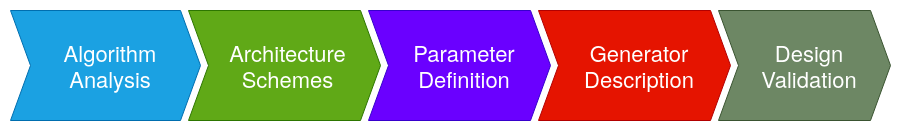
\includegraphics[width=1.0\textwidth]{Figures/Methodology-metadesign}
        \caption{Méthodologie de méta conception}
        \label{ch.resume:sec.exploration:fig.metadesign}
    \end{figure}

    Dans un deuxième temps, nous nous intéressons au processus d'exploration de ces espaces de conception, et proposons la {\bf méta exploration}, une méthodologie d'exploration qui se basent sur la {\bf méta conception}.
    Cette méthodologie repose encore une fois sur l'expertise des développeurs afin de maximiser la flexibilité et la généricité de l'approche (Fig. \ref{ch.resume:sec.exploration:fig.metaexploration}).
    Nous discutons de l'utilisation du paradigme de programmation fonctionnelle\footnote{Chisel étant un langage basé sur scala, proposant donc des fonctionnalités de programmation fonctionnelle} pour la définition des stratégies d'exploration d'espace de conception.
    Plus précisément, nous nous intéressons à une sous classe des stratégies d'exploration, les stratégies séquentielles, et proposons d'utiliser ce paradigme de programmation pour capturer la nature même de composition de ces stratégies.
    Ainsi, nous proposons de considérer les stratégies d'exploration comme une composition d'étapes basiques qui opèrent sur des espaces de conception, et qui peuvent dont être composées pour construire des stratégies plus complexes.
    Chaque stratégie basique repose à la fois sur les métriques d'intérêt à considérer, sur la façon à utiliser pour les estimer et sur comment comparer les différentes implémentations de l'espace de façon efficace (cela peut reposer sur une comparaison exhaustive de toutes les implémentations afin d'optimiser les critères d'intérêt, mais aussi sur des heuristiques moins complexes afin de réduire la durée des processus d'exploration produits ainsi).

    \begin{figure}[h!]
        \centering
        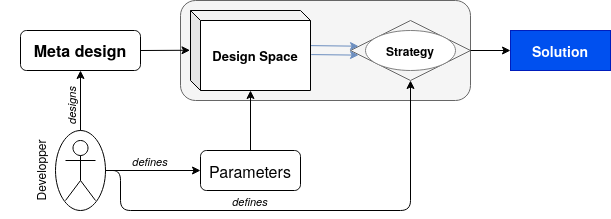
\includegraphics[width=1.0\textwidth]{Figures/Methodology-metaexploration}
        \caption{Méthodologie de méta exploration}
        \label{ch.resume:sec.exploration:fig.metaexploration}
    \end{figure}

    Une formalisation mathématique de cette approche est proposée, afin de faire le lien entre la théorie méthodologique et l'utilisation de la programmation fonctionnelle pour l'implémenter, et plusieurs stratégies basiques sont définies comme preuves de concept.
    Parmi elles, des méthodes classiques d'opération sur des collections (les collections étant ici les espaces de conception à explorer) sont introduites, à savoir les méthodes {\it map} (application exhaustive d'une fonction sur l'ensemble des implémentations qui composent un espace), {\it sort} (un tri de l'espace basé sur l'application d'estimateurs sur l'ensemble des implémentations et sur une relation d'ordre explicite) et {\it prune} (un élagage de l'espace, lui aussi basé sur l'application exhaustive d'une fonction binaire qui défini quelles implémentations doivent être retirées de l'espace de conception, et quelles implémentations doivent rester).
    Nous proposons également deux stratégies plus complexes, basées sur une exploration des voisinages directs des implémentations dans les espaces de conception, afin d’accélérer les processus d'exploration pour les cas d'utilisation où une application exhaustive est infaisable dans un temps raisonnable
    Ces stratégies peuvent donc être utilisées pour réaliser respectivement un tri rapide et un élagage rapide des espaces de conception.

    Dans ce chapitre, nous proposons donc une méthodologie duale d'exploration d'espace de conception qui repose sur l'utilisation de l'expertise des développeurs matériel, permettant de définir des processus d'exploration flexibles et paramétrables, reposant sur la programmation fonctionnelle afin de maximiser l'expressivité des utilisateurs.

\section{Expérimentations et résultats}
\label{ch.resume:sec.expe}
    Afin de démontrer l'utilisabilité de la méthodologie d'exploration d'espace de conception présentée dans les chapitres précédents, un démonstrateur logiciel nommé {\bf QECE} ({\it Quick Exploration using Chisel Estimators}) est proposé dans ce chapitre.
    De plus, la structure interne du logiciel ainsi que les détails intéressants d'implémentation sont décrits pour permettre aux utilisateurs de mieux appréhender les possibilités qu'un tel outil peut apporter au monde de la conception numérique.

    Toujours dans le but de démontrer l'utilisabilité de la méthodologie proposée, un banc d'applications représentatives de l'utilisation des FPGAs en tant que dispositifs d'accélération matérielle est proposé.
    Chaque noyau applicatif composant ce banc a été développé en appliquant la méthodologie de {\bf méta conception}, les détails d'implémentations pouvant être trouvés en annexe du manuscrit en langue anglaise.
    Des expérimentations d'estimation et d'exploration ont été menées sur trois noyaux de ce banc ({\it GEMM}, un algorithme de multiplication de matrices, {\it FFT}, un algorithme provenant du monde du traitement du signal, et {\it Black Scholes}, un modèle de calcul de la valeur d'une action basé sur la méthode de Monte Carlo), afin de mesurer la qualité des estimateurs introduits en Section \ref{ch.resume:sec.estimation}, mais aussi des stratégies d'exploration proposées en Section \ref{ch.resume:sec.exploration}.

    Tout d'abord, nous quantifions l'erreur introduite par les différents estimateurs, démontrant que la méthodologie d'estimation de la consommation des ressources basée sur l'analyse de la représentation intermédiaire introduit une erreur importante par rapport aux résultats des logiciels de synthèses, mais que les métriques estimées peuvent tout de même être utilisée pour inférer la qualité des implémentations considérées en première approche.
    En revanche, nous démontrons que la méthodologie d'estimation des chemins critiques des circuits, basée elle aussi sur une analyse de la représentation intermédiaire, produit des résultats très éloignés de la réalité (à savoir, les résultats du logiciel de synthèse logique), très peu fiables, et en un temps qui peut être plus élévé que les outils propriétaires que l'on cherche à approximer.
    De ce fait, cette approche est laissée de côté comme piste d'amélioration du logiciel proposé, et les estimations de chemins critiques et de fréquences maximale d'opération utilisées dans la suite de nos travaux sont basées sur l'analyse des rapports des outils de synthèse logiques, bien plus fiables mais pouvant être coûteux en temps et en ressources de calcul.
    Enfin, nous démontrons l'utilisabilité de la méthodologie empirique d'estimation de la qualité de service des circuits sur un exemple simple (calcul d'un produit scalaire), afin de montrer comment l'instrumentation des différents moteurs de simulation disponibles dans le flot de conception Chisel peuvent permettre d'estimer des métriques intéressantes, pour certains cas d'utilisation.

    Après avoir abordé l'aspect qualitatif des différents estimateurs proposés, et démontré leurs utilisabilités, nous nous intéressons maintenant à démontrer l'intérêt de l'approche fonctionnelle pour résoudre le problème de l'exploration d'espace de conception, en proposant et en comparant différentes stratégies de {\bf méta exploration} comme définies dans le Section \ref{ch.resume:sec.exploration}.
    Tout d'abord, nous comparons trois stratégies d'exploration sur le noyau applicatif {\it GEMM}, démontrons qu'une approche basée sur l'utilisation de l'expertise du développeur peut permettre de réduire d'un facteur 4 le temps passé pour explorer un espace restreint (42 implémentations) de façon efficace, comparé à une solution par "force brute" consistant à synthétiser toutes les implémentations disponibles.
    Nous démontrons ensuite, sur le noyau applicatif de Transformée de Fourier Rapide ({\it FFT}), qu'une des limites de cette approche d'exploration est la possibilité d'exprimer des relations d'ordres claires entre les implémentations qui composent l'espace de conception, c'est à dire utiliser les métriques d'intérêts disponibles pour définir comparer la qualité des implémentations dans un cas d'utilisation donné.
    Sans modèle applicatif adéquat, il est impossible de comparer, par exemple, des noyaux qui considèrent différentes tailles d'élements dans les calculs, puisque des éléments plus grands vont augmenter la qualité de service des circuits générés, mais également la consommation de ressources --- c'est donc au développeur de spécifier exactement cette relation d'ordre, qui ne peut être implicite.
    Ainsi, sur ce noyau applicatif, nous démontrons que les stratégies avancées d'exploration peuvent s'avérer moins performantes (en terme de temps) que la stratégie par "force brute", dans le cas où le modèle applicatif fourni est trop faible pour exposer des espaces de conceptions suffisamment large pour bénéficier de cette approche.
   Enfin, et pour palier ce problème, nous proposons une stratégie d'exploration de l'espace de conception des noyaux {\it Black Scholes}, basée sur une approche en deux temps: tout d'abord, l'utilisation d'une approche empirique pour estimer la qualité de service (l'erreur introduite par l'implémentation matérielle par rapport à une référence logicielle) et discriminer toutes les implémentations qui introduisent une erreur trop importante, avant de parcourir les implémentations restantes pour sélectionner celle qui proposent le meilleur débit possible, pour la carte FPGA cible. 
    Une telle stratégie peut être définie en une dizaine de ligne dans le logiciel {\bf QECE}, démontrons à la fois l'intérêt et la concision de l'approche fonctionnelle pour l'exploration d'espace de conception.

    Dans ce chapitre, nous démontrons l'utilisabilité de la méthodologie de {\bf méta exploration}, contribution principale de cette thèse, à travers l'usage d'un logiciel démonstrateur ({\bf QECE}) que nous avons développé, et de multiples expérimentations sur des noyaux applicatifs également développés par nos soins.
    L'accent est mis sur l'utilisation de l'expertise des développeurs matériels pour proposer des stratégies intelligentes qui convergent rapidement pour les cas d'utilisation considérés.

\section{Conclusion}
\label{ch.resume:sec.conclusion}
    Dans ce travail de thèse, nous nous intéressons au paradigme émergent des langages de construction matérielle, dont Chisel est un exemple, afin d'améliorer la productivité des développeurs matériel.
    Plus précisément, nous proposons une approche originale pour résoudre le problème de l'exploration d'espace de conception, qui se base sur une méthodologie innovante de conception couplée à l'utilisation du paradigme de programmation fonctionnelle afin de définir des stratégies d'exploration intelligentes, car définies par les développeurs eux mêmes.

    Nous démontrons l'utilisabilité d'une telle méthodologie à l'aide d'un logiciel développeur, nommé {\bf QECE}, que nous avons développé pour l'occasion, qui propose une bibliothèque de méthodologies d'estimation de métriques d'intérêt pour les circuits considérés, et une bibliothèque de stratégies basiques d'exploration qui peuvent être composées pour construire des stratégies plus complexes et adaptables aux différents cas d'utilisation.
    Cette approche permet une grande flexibilité d'utilisation, afin d'être réutilisable et adaptable à de nouveaux cas d'utilisation, améliorant ainsi la productivité des concepteurs numériques.

%%%%%%%%%%%%%%%%%%%%%%%%%%%%%%%%%%%%%%%%%%%%%%%%%%%%%%%%%%%%%%%%%%%%%%%%%%%%%%%%%
%%%%%%%%%%%%%%%%%%%%%%%%%%%%%%%%%%%%%%%%%%%%%%%%%%%%%%%%%%%%%%%%%%%%%%%%%%%%%%%

\cleardoublepage

%---------------------------------------
% Appendix
%---------------------------------------
\appendix
% Add an appendix section explicitly to toc
\addtocontents{toc}{\protect\contentsline{chapter}{Appendixes}{}{}}
\pdfbookmark{Appendixes}{appendixes}
\begin{sectionBegin}
    APPENDIXES
\end{sectionBegin}
~
\pagestyle{empty}
\clearpage

%---------------------------------------
% Appendix sources
%---------------------------------------
% Appendix style 
\pagestyle{fancy}
\fancyhf{}
\fancyhead[LE]{\textsc{\nouppercase{\leftmark}}}
\fancyhead[RO]{\textsc{\nouppercase{\leftmark}}}
\fancyfoot[C]{\thepage}

%-------------------------------------------------------------------------------
\chapter{Chisel Basics}
\labelchapter{app.chisel}
    This Appendix provides motivations about technological choices that were made for this thesis, as well as some insights about basic usage of \chisel, the chosen \myLongAc{HCL}{Hardware Construction Language}.

    Doing so, we aim at providing more information about the usage of \myAcs{HCL} for hardware development.
    A particular focus is put on highlighting some notable differences with the standard \myLongAcs{HDL}{Hardware Description Language} such as \vhdl{} or \verilog{}, in order to help readers that may be familiar with such languages to comprehend the improvements that this paradigm enables.

    \section*{Motivation}
        \myLongAcs{HCL}{Hardware Construction Language} are a novel paradigm which enables the development of parametrized hardware generators instead of dedicated hardware accelerators, as described in Section \ref{ch.problem:sec.hardware:ssec.hcl}.
        Such initiatives are based on high level languages such as \python{} \cite{lockhart_pymtl_2014}, \haskell{} \cite{baaij_clash_2010} or \scala{} \cite{bachrach_chisel_2012}, which enable leveraging novel software constructs for hardware development.

        In this context, we chose to base this work on the usage of \myLongAc{Chisel}{Constructing Hardware in a Scala Embedded Language}, an \myAc{HCL} developed at Berkeley since 2012.
        Since its creation, \chisel{} has been widely adopted by both academic and industrial worlds, with initiatives such as the Rocket Chip generator \cite{asanovic_rocket_2016}, an in-order generator of RISC-V cores, the \myLongAc{BOOM}{Berkeley Out-of-Order Machine} generator \cite{celio_berkeley_2015}, an out-of-order version, or the development of Google \myLongAc{TPU}{Tensor Processing Unit} \cite{google_tpu_2018}.

        Moreover, Chisel has also been used as a basic tile of the Chipyard project \cite{chipyard_berkeley}, a set of tools used to create an agile framework for hardware development, along with tools such as Hammer \cite{wang_hammer_2018}, which decouples physical design concerns, logical design concerns, tool concerns and technology concerns, and Diplomacy \cite{cook_diplomatic_2017}, which enable automatic negotiation of parameters when generating complex Systems-on-a-Chip (SoC).
        It proves that Chisel ever growing community works to ever improve the language features, and that it can be used in wild, complex initiatives.

    \section*{Basic usage}
        To begin with, a simple cheat sheet is available in the project, in order to give some insights about available primitives for hardware generation \cite{chisel_cheatsheet_2021}.

        However, as an exhaustive comprehension of available constructs is not mandatory to understand the content of this work, examples of \chisel{} usage will be provided thereafter that should be sufficient to comprehend the improvements brought by \myAc{HCL} usage.

        \subsection*{Chisel compilation flow}
            The \chisel{} \myLongAc{HCF}{Hardware Construction Framework} structure is based on a separation of concerns inherited from the structure of software compilers, where the entry point ({\bf frontend}) and the tool output ({\bf backend}) are separated by an \myLongAc{IR}{Intermediate Representation}.
            Such architecture allows to implement support for various input and target languages, while exhibiting a modular structure for the developers.

            An example of a \chisel-based generation of a parametrized increment module is introduced in Figure \ref{app.chisel:fig.incr}, where two simple parameters are exhibited: the width of the module output, and its initialization value.

            Three main steps are taken during the generation of this module:
            \begin{enumerate}
                \item The \chisel{} parameters are resolved during the elaboration, meaning that the parameters are fixed for the remaining of the flow.
                    This is similar to the \verilog{} elaboration process where the explicit module parameters are resolved and propagated in the circuit description.

                    A {\bf high level} \firrtl{} representation is here generated as a first \myAc{IR}.
                \item Multiple transforms (including verifications such as combinatorial loop detection) are run over the \firrtl{} representation, progressively lowering the abstraction level, until a {\bf low level} representation is produced.

                    At the end of this process, all the data types and widths have been resolved, the conditional statements have been replaced, and it is guaranteed that every component is connected exactly once.\footnote{As the example module is very simple, no significant differences are exhibited between {\bf high} and {\bf low level} \firrtl{} representations.}

                    One can remark that, at this step, the parameters are fixed (\eg the width of the output is fixed to 8 bits) and implicit control signals --- \ie the clock and the reset --- have been generated automatically.
                \item The last step is a simple translation, where the {\bf low} \firrtl{} is translated to \verilog{}.

                    As the abstraction level remains the same, this process is quite straightforward, with the simple goal of providing an output language that can be used by most tools in the industry.
            \end{enumerate}

        \begin{figure}[h!]
            \centering
            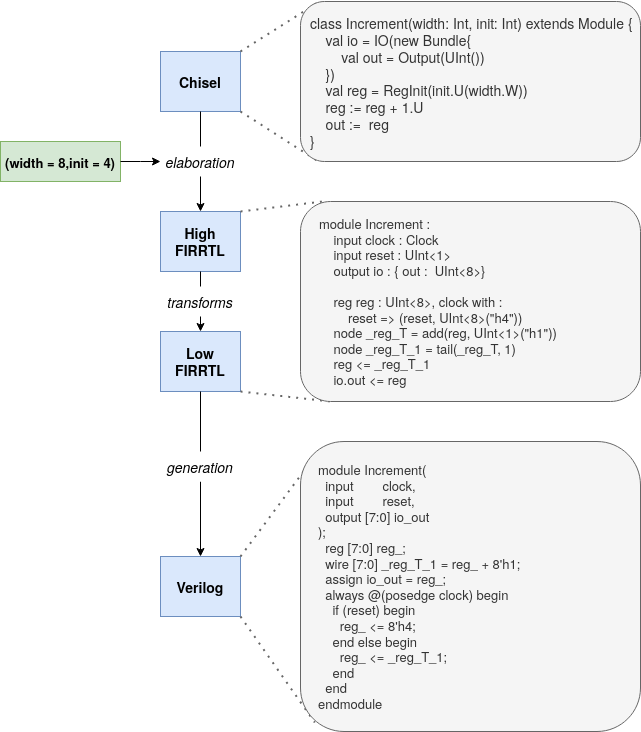
\includegraphics[width=1.0\textwidth]{Figures/flow-example}
            \caption{Implementing an increment module using \chiselT}
            \label{app.chisel:fig.incr}
        \end{figure}

        \subsection*{Exposing high level parameters at constructor level}
            One of the main differences of \myAcs{HCL} with standard \myAc{HDL} is the possibility to leverage \myLongAc{OOP}{Object-Oriented Programming} features --- such as module inheritance --- for hardware construction.
            While evolutions of those languages have come with a way to define simple \lstinline{parameter}s for module generation, as well as \lstinline{generate} features which enable loop based generation of hardware, it remains difficult to leverage complex parameters that could bring a lot for hardware generation.

            A simple example of a \chisel{} generator is introduced in Listing \ref{app.chisel:list.adder}, implementing a type parametric adder generator.
            It leverages a \scala{} constructor for module definition, allowing to define how each constructor parameter is used for adder generation --- meaning that the type of \lstinline{op1}, \lstinline{op2} and \lstinline{res} ports will be defined at elaboration time only. %\footnote{The process used to generate \verilog{} code from a \chisel{} {\bf Module} instance is called {\bf elaboration}. It consists in the iterative resolution of top level parameters, before running various \firrtl{} transforms in order to generate \myAc{RTL} code.}
            This code can then be used to generate variations of an adder module, allowing to instantiate an adder on 32 bit wide unsigned integers (line 14.) or on 8 bit fixed point numbers (line 15.) with the same description.

            Used parameter is here defined using the template feature from \scala, using a \lstinline{T} type for generation.
            This type is then checked at elaboration, to verify that it does implement the \lstinline{Data} type (the basic type for any data in \chisel) as well as the \lstinline{Num} trait (which ensure that a given type does implement basic arithmetic operations such as addition and multiplication).
            Doing so, one can leverage {\it polymorphism} to generate modules operating on any type that fits the requirements, enabling to build a library of easy to use components that can be adapted to multiple use cases.

            While this example is intentionally kept simple for the reader to understand the provided code, it should be noted that providing a similar module using standard \myAc{HDL} would require either to copy and adapt the code for every possible type, or search and replace type specific operations in the code.
            Moreover, more complex parameters can be defined, such as high-order functions which can be used as module parameters to change the behaviour of a circuit in functional fashion.

            \begin{figure}[h!]
                \begin{lstlisting}[numbers=left,stepnumber=1,
                                   caption={Type parametric adder generator in \chiselT},
                                   label={app.chisel:list.adder}]
import chisel3._
import chisel3.experimental.FixedPoint

class Adder[T <: Data with Num[T]](tpe: T)
    extends Module {
    val io = IO(new Bundle({
        val op1 = Input(tpe)
        val op2 = Input(tpe)
        val res = Output(tpe)
    })

    io.res := io.op1 + io.op2
}   

val uintAdder = new Adder(UInt(32.W))
val fpAdder = new Adder(FixedPoint(8.W, 3.BP))\end{lstlisting}
            \end{figure}

        \subsection*{Using functions as block generators}
            Another interesting feature of \chisel{} is the ability to generate hardware using functions to provide block abstractions --- in other terms, calling a function can result in \myAc{RTL} code generation at the end of the elaboration.

            \begin{figure}[h!]
                \vspace{-0.85cm}
                \begin{subfigure}{1.0\textwidth}
                    \begin{lstlisting}[language=Verilog,
                                       caption={Behavioural description of a register in Verilog},
                                       label={app.chisel:fig.register:list.verilog}]
module register (parameter WIDTH) (
    input clk,
    input reset,
    input [WIDTH-1:0] D,
    output [WIDTH-1:0] Q);

    reg [WIDTH-1:0] myregister;
    always @(posedge clk) begin
        if (reset)
            Q = 0;
        else
            Q = D;
endmodule\end{lstlisting}
                \end{subfigure}
                \begin{subfigure}{1.0\textwidth}
                    \begin{lstlisting}[caption={Building a register using \chiselT{} constructs},
                                       label={app.chisel:fig.register:list.chisel}]
class MyRegister[T: Data](tpe: T) extends Module {
    val io = IO(new Bundle{
        val dataIn = Input(tpe)
        val dataOut = Output(tpe)
    })
    // register width is inferred from dataIn type
    val myRegister = RegNext(dataIn)
    dataOut := myRegister
}\end{lstlisting}
                \end{subfigure}
                \caption{Building a register: HDL \vs{} HCL}
                \label{app.chisel:fig.register}
                \vspace{-0.55cm}
            \end{figure}

            This includes {\bf constructor methods}, meaning that the instantiation process can be leveraged to generate behavioural description of circuit.
            A simple example is provided in Figure \ref{app.chisel:fig.register}, where a \verilog{} description of a register (List. \ref{app.chisel:fig.register:list.verilog}) is compared to its \chisel{} counterpart (List. \ref{app.chisel:fig.register:list.chisel}).

            As can be observed here, the semantic for describing a register in standard \myAc{HDL} is based on simulation needs, as those languages were originally designed for simulation purposes instead of hardware description.
            One then needs to declare a logic signal (line 6.), and a process sensitive to the clock signal to either update the value, or reset it (lines 7-11).

            While every hardware developer has grown used to such way to describe registers, it remains a verbose way to describe a basic component that will be instantiated hundreds of times in a single circuit.
            Moreover, this semantic is quite confusing for beginners, as \verilog{} exposes a \lstinline[language=Verilog]{reg} keyword for signal declaration, but that does not actually differ from the \lstinline[language=Verilog]{wire} keyword from a semantic point of view.\footnote{The only way to describe a register is to use specific patterns such as the one in Listing \ref{app.chisel:fig.register:list.verilog}, that will be recognized and translated by synthesis tools to instantiate actual hardware registers.}

            On the other hand, \chisel{} leverages block generation through function calls, enabling users to simply instantiate basic classes for register description (line 6.).
            Once it is done, assigning a signal to the register value (\ie \lstinline{myRegister} value at line 6.) will change the next value (as does changing the value on port \lstinline{D} in List. \ref{app.chisel:fig.register:list.verilog}), while using the variable as a right-hand operand (line 7.) is equivalent to reading the content of the register (\lstinline{Q} port).

            This simple semantic is less error prone, as it does not rely on a copy of a particular pattern for instantiation, and allowing easier instantiation of basic component is a key feature to allow developers to spend more time on actual design problems, thus improving their productivity.
            We also see here that using high level parameters as exposed in previous section can enable to build highly reusable component generators, by defining a type parametric register module for example.

            \underline{Remark:} Both \lstinline{clk} and \lstinline{reset} signals are not provided for register instantiation in the \chisel{} example.
            In fact, those signals are implicit in any class inheriting from \lstinline{Module}, the basic class for hardware circuits.
            They are used for instantiations of components that require them, and are being propagated to every instantiated sub module in order to expose coherent time zones to users.
            If needed, they can be overwritten manually to build different time zones --- \eg for circuits using multiple clock domains.

        \subsection*{Leveraging high level constructs for generation}
            The last feature that we will consider here is the usage of high level functionalities for hardware generation.

            As \chisel{} is based on \scala{} language, features from this language can be used to define module generators and bring more expressivity for developers.

            \begin{figure}[h!]
                \begin{lstlisting}[caption={Building a dot product kernel using \chiselT},
                                   label={app.chisel:list.mac}]
class DotProduct(width: Int, nElem: Int) extends Module {
    val dataType = UInt(width.W)

    val io = IO(new Bundle{
        val op1 = Input(Vec(nElem, dataType))
        val op2 = Input(Vec(nElem, dataType))
        val out = Output(dataType)
    })

    io.out := ((io.op1 zip io.op2)
        .map{ case (a, b) => a * b })
        .reduceTree(_ + _) // use balanced tree
}\end{lstlisting}
            \end{figure}

            Listing \ref{app.chisel:list.mac} introduces a {\bf dot product} generator parametrized by elements width and number.
            This generator thus accepts two vectors of elements, which elements are multiplied two by two, before being summed to produce the output.
            Such operation can be captured using the {\bf map-reduce} paradigm, as it would be done in a software implementation leveraging functional programming, and hardware designers should also benefit from such programming patterns.

            An example of the target architecture is provided in Figure \ref{app.chisel:fig.dot}, to help the reader to understand the gap between the final circuit, and what the designer actually requires to describe using either \chisel{} or \verilog.

            Lines 9. to 11. expose how \chisel{} can be leveraged to build a generator for such implementations: input vectors are {\bf zipped} --- \ie elements of each vectors are paired --- before multiplication is applied to each pair.
            Resulting vector is then reduced through add operations, using a binary tree structure to force elaboration to produce a balanced adder tree.

            \begin{figure}[h!]
                \begin{lstlisting}[language=Verilog,basewidth={0.5em, 0.4em},tabsize=2,numbers=none,xleftmargin=-2mm,
                                   caption={Dot product generic implementation in Verilog},
                                   label={app.chisel:list.verilogDP}]
module dot_product #(
    parameter NELEM,
    parameter WIDTH,
  ) (
    input [N-1:0] [WIDTH-1:0] op1,
    input [N-1:0] [WIDTH-1:0] op2,
    output        [WIDTH-1:0] out,
  );

  localparam  STAGES = clog2(NELEM);
  localparam  NPADDED = 2**(STAGES);

  wire  [STAGES:0] [NPADDED-1:0] [WIDTH-1:0] tab;

  generate
    // Init loop with mul (required padding for NELEM not power of 2)
    for (i=0; i<NPADDED; i=i+1) begin:init
      // 0 padding is fine for add reduce
      assign tab[0][i] = (i < NELEM) ? op1[i] * op2[i] : '0;
    end

    // main reduce loop with tree
    for (stage=0; stage<STAGES; stage=stage+1) begin:stages
      for (couple=0; couple<2**(STAGES-stage-1); couple=couple+1)
        begin:couples
          localparam first  = couple * (2**(stage+1));
          localparam second = first + (2**stage);
          assign tab[stage+1][first] =
            tab[stage][first] + tab[stage][second];
      end
    end
  endgenerate

  assign out = tab[STAGES][0];
endmodule\end{lstlisting}
            \end{figure}

            A \verilog{} counterpart is proposed in Listing \ref{app.chisel:list.verilogDP}, to exhibit the complexity of building such generator in a traditional \myAc{HDL}.
            To do so, we require to expose a multidimensional array of elements and populate it according to some specific patterns on the indexes, through the \lstinline[language=Verilog]{generate ... for} construct.
            This pattern is hence recognized by the synthesis tool, which eliminates the useless elements of the array, and build the correct adder tree.

\clearpage
            A last remark can be done on the differences between those two paradigms: while changing the data path of the \verilog{} module --- \eg to add registers after multipliers and adders --- requires to modify the whole code, it can be done in a functional way in the \chisel{} description.

            This is possible because both \lstinline{map} and \lstinline{reduceTree} functions accept high-order functions as parameters to define which operations are to be performed, which is known in the software world as {\bf functional programming}.
            In fact, the \lstinline{reduceTree} construct even accepts a second function as parameter, to define what to do on non balanced trees (when the number of elements is not a power of two), allowing to define a simple delay using a \lstinline{RegNext} in the case of pipelined additions, for instance.

            This final example thus exhibits how the introduced features enable to build efficient hardware generators which are easier to design, understand and adapt to new use cases.

            \begin{figure}[h!]
                \centering
                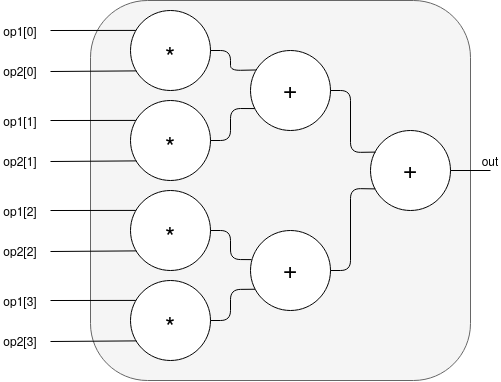
\includegraphics[width=1.0\textwidth]{Figures/dot-archi}
                \caption[Example of a dot product architecture to generate]{Example of a dot product architecture to generate\newline ({\it using vectors of 4 elements})}
                \label{app.chisel:fig.dot}
            \end{figure}
            


\cleardoublepage
%-------------------------------------------------------------------------------
\chapter{Benchmark Composition}
\labelchapter{app.benchmark}

    In order to analyse how the defined methodologies can be leveraged to improve the life of hardware developers, we implemented {\bf 7 computation kernels} using \chisel, which are introduced in Table \ref{app.benchmark:table.benchmark}.

    Each kernel has been developed by applying the {\bf meta design methodology} introduced in section \ref{ch.dse:sec.definition:ssec.meta}, and this appendix also exposes --- in addition to the benchmark description --- which considerations were taken into account, for each kernel, in order to provide an explorable meta design from a prior algorithmic analysis. 

    This benchmark is proposed as an open-source project \cite{ferres_benchmark_2021}.

    \section*{Kernel model}
        The kernels were built to be integrated in a simple programming model, by exposing a unified interface.
        To do so, we defined a \chisel{} {\bf Role} and {\bf Shell} based architecture, as can be seen in emerging \myLongAc{FPGA}{Field-Programmable Gate Array} projects that aim at separating the accelerators implementation from their interfaces \cite{caulfield_cloud-scale_2016}.

        The proposed interface is kept simple, as {\bf Role} simply exposes a bi-directional {\bf Ready/Valid} interface with a parametric {\it bandwidth} (Fig. \ref{app.benchmark:sec.kernel:fig.model}), that can be then be integrated in more or less complex {\bf Shells}, ranging from simple mapping of this \myLongAc{IO}{Input/Output} to the communication \myLongAc{IP}{Intellectual Property} that may be available on the target board, to complex communication protocols.

        However, such structure is quite simple, and evolutions should consider integrating multi-lane communications for configuration purposes --- which are currently done using the same \myAc{IO} bus, meaning that the accelerators must consider configuration in their data communication protocols.

    \clearpage
        \begin{figure}[ht!]
            \centering
            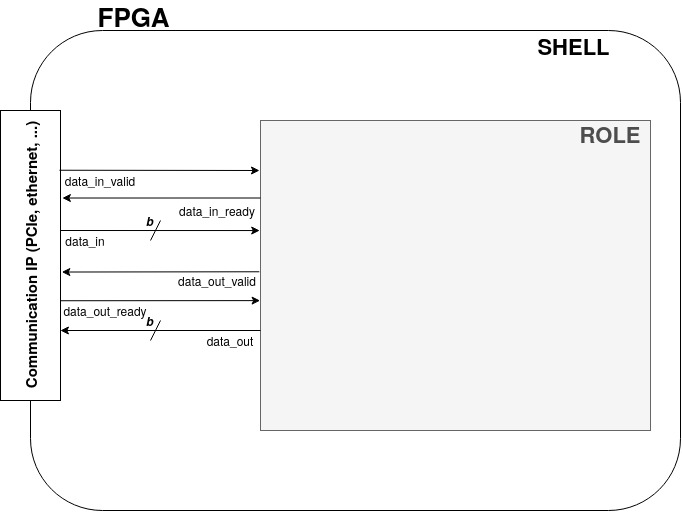
\includegraphics[width=0.9\textwidth]{Figures/shell.png}
            \caption{Simple Role and Shell model used}
            \label{app.benchmark:sec.kernel:fig.model}
        \end{figure}
        \vspace{-1cm}

    \section*{Dot Product}
        The dot product generator has been developed as a simple example, and does not expose a heavy design space.
        Moreover, an example of the target architecture is introduced in Figure \ref{app.chisel:fig.dot}.

        Given two vectors $a$ and $b$ of dimension $n$, we compute:
        \begin{equation}
            \label{app.benchmark:sec.dp:eq.formula}
            c = \sum_{i=0}^{n-1}a_i*b_i
        \end{equation}

        
        The {\it Vector width} is used to define the algorithmic complexity of the implementation, while both {\it dynamic} and {\it precision} define the element type to operate on.
        In order to take advantage of an \myAc{FPGA} implementation, we aim at exploiting the parallelism of the algorithm, while keeping the resource usage under given constraints.
        The dot product can easily be expressed in a functional way, using the {\bf Map-Reduce} pattern, implying we can extract a maximum parallelism level of $n$, by performing all the multiplications in parallel before performing reduction through additions.
        We thus expose {\it parallelism} as a parameter, allowing the user to easily increase the throughput at the cost of functional unit replication.

    \clearpage
    \section*{General Matrix Multiply}
\vspace{-0.2cm}
        The \myLongAc{GEMM}{General Matrix Multiply} algorithm is a generalization of the matrix multiply algorithm.

        Given three matrices $A$, $B$ and $C$ in $\mathcal{M}_n$, the set of the matrices of dimension $n \times n$ (that we consider square for simplification) and two values $\alpha$ and $\beta$, we compute:
        \begin{equation}
            \label{app.benchmark:sec.gemm:eq.formula}
            C = \alpha \cdot A \times B + \beta \cdot C
        \end{equation}
        A meta design for the \myAc{GEMM} algorithm has been introduced in prior work \cite{ferres2020chisel} --- from which Equation \ref{app.benchmark:sec.gemm:eq.throughput} is extracted --- and was manually explored in order to demonstrate how both {\bf meta design} and {\bf meta exploration} can be leveraged to increase designers productivity \cite{ferres_2021_integrating}.

        The \myAc{GEMM} generator has been developed in order to maximize the \myAc{IO} usage, targeting a temporal behaviour as represented in Figure \ref{app.benchmark:fig.gemm-chrono}.
        Such prior analysis enables to build a generic generator that uses both \myLongAc{BRAM}{Block Random-Access Memory} and \myLongAc{MAC}{Multiply and Accumulate} to build adaptable designs that will compute partial results on the fly, resulting in a theoretical maximal usage of the bus.

        \begin{figure}[h!]
            \center
            \scalebox{.8}{
                \begin{wave}{5}{14}
                    \nextwave{ready} \bit{1}{14} \bit{0}{1}
                    \nextwave{input} \known{$\alpha$}{1} \known{$\beta$}{1} \known{$C$}{4} \known{$B^t$}{4} \known{$A$}{4} \bit{0.5}{1}
                    \nextwave{valid} \bit{0}{11} \bit{1}{4}
                    \nextwave{output} \unknown[XXX]{11} \known{$result$}{4}
                    \nextwave{} \duration{$\Delta_c$}{15}
                \end{wave}
            }

            \caption{Targeted chronogram for an efficient GEMM implementation}
            \label{app.benchmark:fig.gemm-chrono}
        \end{figure}
\vspace{-0.3cm}
        Equation \ref{app.benchmark:sec.gemm:eq.throughput} introduces the theoretical throughput (in $operation\cdot second^{-1}$) of the designs generated from this description, and is used to define a cost function to be maximized while exploring the \myAc{GEMM} design space.
        One can remark that doing this enable to normalize a cost metric through different matrices dimensions, as performing {\bf one \myAc{GEMM} computation} over $\mathcal{M}_n$ is comparable to performing {\bf eight $\mathcal{M}_{\frac{n}{2}}$ computations}.

        \begin{equation}
            \label{app.benchmark:sec.gemm:eq.throughput}
            T_{GOp/s} = \frac{f}{\Delta_{cycle}} = \frac{2 \times n^3 \times f \times b}{3 \times n^2 \times e}
        \end{equation}

        As a result, we define three parameters for \myAc{GEMM} generation: the {\it bus bandwidth}, which defines the capacity of the \myAc{IO} bus, the {\it element bit width}, which defines the size of each element in the considered matrices --- meaning that $\frac{bandwidth}{bitwidth}$ element can be sent and received each cycle --- and finally the {\it dimension} (or $n$) of the matrices in $\mathcal{M}_n$.

    \clearpage
    \section*{Fast Fourier Transform}
        The \myLongAc{FFT}{Fast Fourier Transform} algorithm is used in signal processing to provide frequency analyses from temporal data.

        Given $x_0, ..., x_{n-1} \in \mathbb{C}$, \myAc{FFT} is computed using the following formula:
        \begin{equation}
            \label{app.benchmark:sec.fft:eq.formula}
            f_j = \sum_{k=0}^{n-1}x_k e^{-\frac{2\pi i}{n}jk}
        \end{equation}

        The \myAc{FFT} generator was built to maximize the \myAc{IO} bus usage, resulting in a pipelined implementation inspired from Gerez \cite{gerez_fft_2012}.

        The pipeline is based on the \myLongAc{R2MDC}{Radix-2 Multi-Path Delay Commutator} technique \cite{rabiner1975theory}, using multiple Radix-2 stages to reduce the \myAc{FFT} problem size by 2 at each stage, in a {\it divide and conquer} fashion.
        We use the \myLongAc{DIF}{Decimation In Frequency} mode in order to consume input data (temporal samples) in a \myAc{FIFO} fashion, resulting in a need to reorder the output data (frequency samples) at the end of the pipeline.
        This is done by using a {\bf Ping Pong buffer}, which enables to provide the frequency data in a coherent order, even if the \myAc{DIF}-based implementations produce out-of-order frequency samples --- moreover, using another {\bf Ping Pong buffer} on the \myAc{R2MDC} inputs enables to exploit them at 100\%.
        The {\bf Twiddle factors} --- \ie the trigonometric coefficients --- are computed {\it a priori} and stored in \myLongAc{ROM}{Read-Only Memories} to fasten the computations.

        This pipelined implementation allows to maximize the \myAc{IO} bus usage as we consume input data on the fly, while maximizing the resource usage.

        The \myAc{FFT} generator relies on three parameters: the {\it parallelism} level, which defines the number of lanes used in the \myAc{R2MDC} model --- \ie the number of inputs that can be absorbed in one cycle in the generated accelerator --- the {\it element bit width}, which defines the size of each complex element used for computation, and the {\it size} of the \myAc{FFT} problem being solved.
        As for the {\it element bit width}, the \myAc{FFT} uses {\bf Fixed Point} representation for the computations, and one could want to explore this representation by defining both {\it dynamic} and {\it precision} parameters. 
        However, as we do not focus \myLongAc{QoS}{Quality of Service} based exploration on this kernel, we chose to define the data representation using only one parameter --- we use $\frac{bit width}{2}$ as values for both {\it dynamic} and {\it precision}.

        We can remark that, in contrast with the \myAc{GEMM} implementations, two \myAc{FFT} implementations of different sizes cannot be compared easily, as the first one cannot be expressed by composing instances of the second one.
        We here solve different applicative problems, hence the developers either need to specify which size to use, or to allow the exploration process to make this decision through applicative information (\eg \myAc{QoS}).

    \section*{Finite Impulse Response Filter}
        \myLongAc{FIR Filter}{Finite Impulse Response Filter} is a standard digital processing algorithm, based on the application of a finite number of coefficients to temporal samples in order to modify an input signal.

        % Given a set of coefficients $c_0, ..., c_{n-1}$ and time indexed samples $x_t, t\in [\![0; +\infty ]\!]$
        The filter response is computed using a discrete convolution between an input signal $x[t]$ and the function represented by $c_k, k\in [\![0, n-1]\!]$ coefficients:
        \begin{equation}
            \label{app.benchmark:sec.fir:eq.formula}
            f(t) = \sum_{k = 0}^{n-1} c_k \times x[t - k]
        \end{equation}

        Once again, we aim at exploiting the \myAc{IO} bus at its maximal capacity by absorbing the whole input bandwidth as temporal samples at each cycle.
        To do so, a structured buffer is built to enable windowed accesses to the buffer data: if we consider that $k$ elements are presented on the input bus at each cycle, then those $k$ elements $e_i, i \in [\![0, k-1]\!]$ are fed to a \myAc{FIFO}. 
        On read, this structure enables to access $k$ different vectors for inputs ($[\![e_{i}, e_{i+k-1}]\!], i \in [\![0, k-1]\!]$), meaning that we can compute $k$ successive response of the filter $f(t+i), i\in[\![0, k]\!]$ in parallel.
        Doing so, we hence built a parametrizable, fully pipelined \myAc{FIR Filter} generator that takes the best of the available \myAc{IO} capacities.

        So built \myAc{FIR Filter} generator uses three parameters: the {\it bus bandwidth}, which defines the capacity of the \myAc{IO} bus, the {\it element bit width}, which defines the data representation used in the computations, and the {\it tap number}, which defines the number of coefficients used in the filter.
        A fourth parameter allows to define whether coefficients are hard-coded --- \ie stored in \myAcs{ROM} --- or provided in the communication protocol. However, no exploration process should consider both kinds of implementations as they are not comparable and depend on both applicative needs and target constraints.

        Here again --- as for \myAc{FFT} implementations comparison through multiple sizes --- it is difficult to compare \myAc{FIR Filter} implementations if the {\it tap numbers} differ.
        However, one could define application specific metrics to allow such comparison, for example by defining applicative needs --- \eg the {\bf filter type} ({\it low-pass}, {\it band-pass}, ...) or {\bf cut-off frequency} --- and running empirical simulations to choose which implementation best fit one's need.
        
    \clearpage
    \section*{Monte Carlo}
        Both {\it Pi} and {\it Black Scholes} kernels are based on a parametric {\bf Monte Carlo} generator, for which the meta architecture is introduced in Figure \ref{app.benchmark:sec.monteCarlo:fig.kernel}.

        In order to provide random samples following normal distributions for the different cores --- which are generated using different seeds --- we use a parametric Tausworthe generator to feed pre-computed {\bf Box-Muller} \myAcs{ROM} \cite{box1958note}.
        Using so defined samples, each core performs the given computations, and the partial results are averaged to provide a statistical value for the result --- for example, we estimate the value of $\pi$ by checking if random points are inside a circle of radius one before computing the proportion of points that are within this disk.
        This can be used to determine the area of the disk, hence we can empirically approximate $\pi$.

        \begin{figure}[h!]
            \centering
            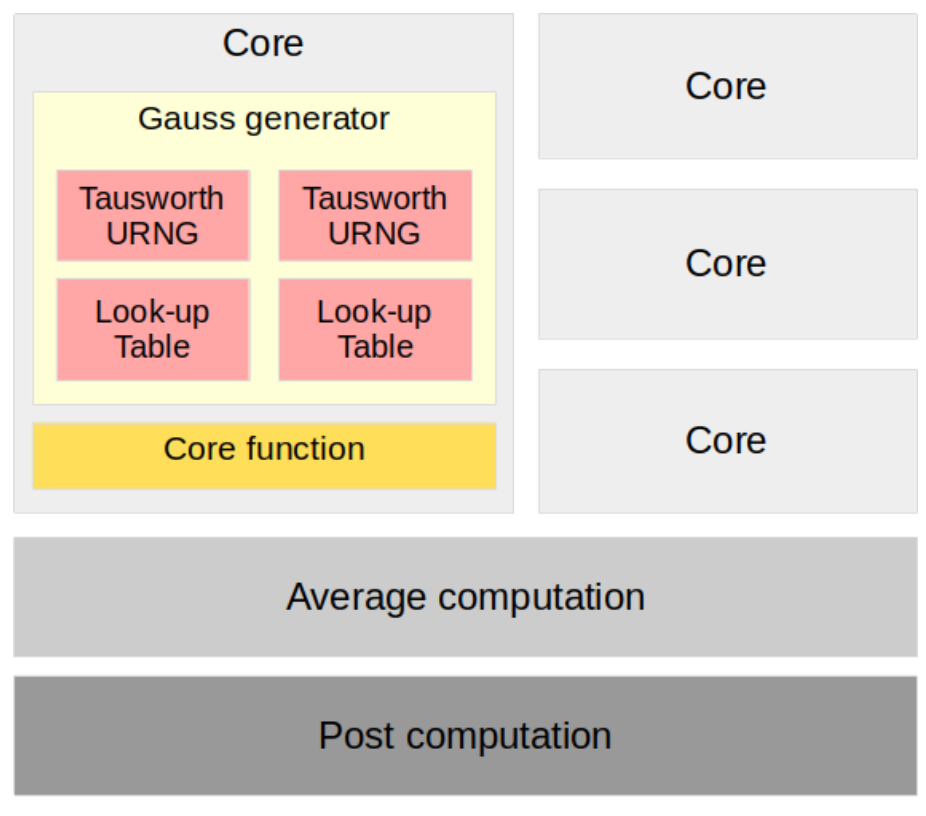
\includegraphics[width=.6\textwidth]{Figures/monteCarloCore.png}
            \caption{Monte Carlo kernel meta architecture}
            \label{app.benchmark:sec.monteCarlo:fig.kernel}
        \end{figure}

        We use a {\bf Factory pattern} to build different {\bf Monte Carlo} kernels, fully exploiting the \myLongAc{OOP}{Object-Oriented Programming} features of \chisel{} for such generators.
        This enables to build both {\it Pi} and {\it Black Scholes} kernels by defining specific inner functions while allowing code reusability by exploiting inheritance.

        For both kernel generators, we thus define four parameters: the {\it dynamic} and the {\it precision} to define the Fixed Point representation for the computations, the {\it iteration number}, which defines the number of experiments to be run before performing both average and post processing to provide a result, and the {\it core number} which defines the number of parallel cores to run iterations.

        As for the {\it Black Scholes} generator, we aim at computing the price of an action at time $t$, given the following equation --- $\mu$, $\sigma$ and $T$ being respectively the {\bf risk free rate}, the {\bf volatility} and the {\bf maturity} of the considered option:
        \begin{equation}
            \label{app.benchmark:sec.monteCarlo:eq.bs}
            S(t) = S(0)\times e^{(\mu - \frac{1}{2}\sigma^2)T + \sigma\sqrt{T}\mathcal{N}(0, 1)}
        \end{equation} 
        
        However, as  hardware-based computations of the exponential function are costly, we leverage {\bf Euler-Maruyama} method to sequentially approximate the formula (Eq. \ref{app.benchmark:sec.monteCarlo:eq.bs}):
        \begin{equation}
            \label{app.benchmark:sec.monteCarlo:eq.bsem}
            S_{\Delta t} = S_0((1 + (\mu - \frac{1}{2}\sigma^2)\Delta t) + \sigma\sqrt{\Delta t}\mathcal{N}(0, 1)
        \end{equation}

        To exploit this approximation model, the {\it Black Scholes} kernels are generated using a fifth parameter, namely the {\it Euler iteration number}, which is used to define how many iterations are taken for each {\bf Euler-Maruyama} based approximation.
        Moreover, other parameters could be considered for exploration, as this meta implementation uses hard coded values for the {\it Black Scholes} specific parameters ($\mu$, $\sigma$ and T), and for the {\bf Monte Carlo} parameters, such as the Tausworthe and the Box-Muller configurations.
        Such values may also be integrated in the communication protocol, in order to build dynamically programmable accelerators.

        For both {\bf Monte Carlo} based kernels, we hence expose heavy design spaces as the \myAc{QoS} is considered for exploration --- we aim at maximizing the design efficiency (\ie performance \vs cost ratio) while insuring that the generated designs does not generate significant errors with respect to a given workload model.

    \section*{Multilayer Perceptron}
        The \myLongAcs{MLP}{Multilayer Perceptron} are simple neural network models that are based on the original Perceptron model as introduced by F. Rosenblatt in 1958 \cite{rosenblatt1958perceptron}.
        They consist on a given number of {\bf fully connected} neuron layers --- meaning that each neuron of a layer $n$ is connected to every neuron of the layers $n - 1$ and $n + 1$.
        
        Such model has been used for more than twenty years for multiple uses, notably for image classification over the {\bf MNIST database} (handwritten digits) \cite{lecun_gradient-based_1998}.
        The \myAc{MLP} implementations are costly, as all the necessary connections result in a complex interconnection model, which led researchers to develop more compact neural network for \myLongAc{DL}{Deep Learning} --- especially for image processing and recognition domains --- such as \myLongAc{CNN}{Convolutional Neural Network} models.
        However, some specific domains still require to use fully connected networks --- \eg personalization and recommendation systems \cite{naumov2019deep} --- and given their simple structure, we chose to implement a \myAc{MLP} generator using \chisel.

        We chose not to base developed generator on the {\bf Role} model as introduced in Figure \ref{app.benchmark:sec.kernel:fig.model}, in order to allow a multi-channel interface model, notably to be able to configure the accelerator through a distinct \myAc{IO} bus.
        In order to take the best of \myAc{FPGA} specificities, we chose to target a {\bf fully unrolled} implementation, meaning that each neuron in the network will be an independent entity with its own memory and computation units --- in contrast to most hardware implementations which are based on scheduling the different neuron tasks on a topology-independent amount of hardware neurons --- as existing works proved that unrolling networks on \myAcs{FPGA} can lead to efficient implementations \cite{prost2017scalable}.

        Most of the design effort was done at {\bf neuron level}, in order to provide efficient basic units for computing neuron outputs.
        Let $N(i, j)$ be the $j^{th}$ neuron of the $i^{th}$ layer of a given network.
        $N(i, j)$ got $n$ different inputs $x_0, ..., x_{n-1}$ resulting from the preceding layer, $n$ different weights $w_0, ..., w_{n-1}$ that result from a prior training of the network and are used for configuration purposes, and a bias $b$ which is also provided by the training phase. 
        An {\bf activation function} $f$ is also applied to each neuron output, and is defined at network level --- thus it does not need to be configured at neuron level as it is defined at elaboration time and can be hard-coded.

        The output $o(i, j)$ is then computed using the following formula:
        \begin{equation}
            \label{app.benchmark:sec.mlp:eq.formula}
            o(i, j) = f(\sum_{k = 0}^{n-1} x_k w_k + b)
        \end{equation}

        A simplified version of the chosen neuron architecture is introduced in Figure \ref{app.benchmark:sec.mlp:fig.neuron}.
        Each neuron is composed of an embedded memory --- which should leverage \myAcs{BRAM} for \Xilinx{} boards --- to store network weights, and a computation unit to perform \myLongAc{MAC}{Multiply and Accumulate} operations.
        As \myAc{MAC} operations can easily be parallelized in a way similar to the dot product, we hence expose a {\it parallelism} parameter at neuron level to easily define the \myLongAc{FU}{Functional Unit} replication factor.
        In order to properly schedule the output propagation, a {\it scan-chain} system is inserted after the activation function, to manage the synchronization with the next layer.

        \begin{figure}[h!]
            \centering
            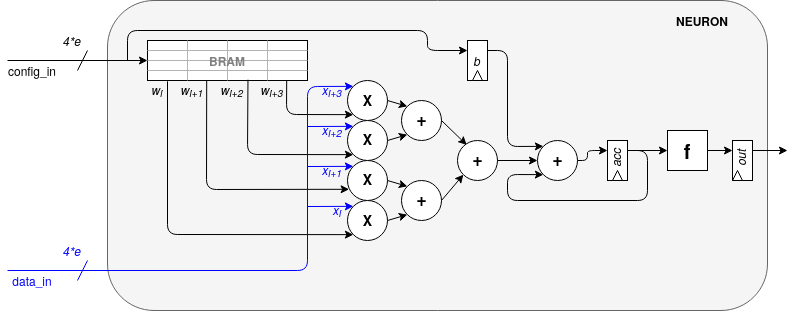
\includegraphics[width=1.0\textwidth]{Figures/neuron.png}
            \caption{Simplified schematic for a neuron implementation}
            \label{app.benchmark:sec.mlp:fig.neuron}
        \end{figure}

        Each neuron also includes a parallel data bus for configuration, which uses a simple \myLongAc{FSM}{Finite State Machine} to write weights in a \myAc{BRAM} --- weights are written in a vector-like structure, enabling to access to $k$ weights $w_0, ..., w_{k-1}$ each cycle, in order to feed $k$ \myAc{MAC} units in parallel.
        
        Using this basic neuron generator, we thus define the whole network as a composition of layers, each layer being defined as a composition of neurons, with small \myAcs{FSM} for the control flow --- including two different \myAc{IO} buses, respectively for the data and the weights.

        We chose to use MNIST as a use case for so defined \myAc{MLP}, as it is both a simple example and a standard reference in image processing.

        Beside the {\it parallelism} parameter, which allows to explore a trade-off between the neuron throughput and its resource usage, we defined three parameters: {\it \#neuron($1^{st}$ layer)} and {\it \#neuron($2^{nd}$)} respectively to define the number of neurons in $1^{st}$ and $2^{nd}$ layers, while the {\it element bit width} once again defines how data are represented in the design.
        We here only explore three layered networks, where the first layer is composed of as many neurons as there are pixesl in an input picture, and the last layer is composed of as many neurons as the number of possible classifications (here, 10 classes for 10 different digits).
        Whereas this means that both input and output layer widths are defined at application level, it also means that this generator can be adapted to any network, and that any number of layers can be put between input and output layers, resulting in a possibly very wide design space to explore.
        Moreover, multiple {\bf activation functions} could be explored using \scala{} functional programming features, enabling to compare either different activation functions or multiple implementations of a same activation function.

        In order to really take advantage of the \myAcs{FPGA} specificities, multiple improvements are considered --- including considering hard-coding the network configuration parameters to reduce memory footprint, various arithmetic possibilities that can be leveraged by changing the data type, and an automatically searching for the best topology.

%-------------------------------------------------------------------------------

    \begin{sidewaystable}[h!]
        \tiny
        \begin{adjustbox}{width=1.0\columnwidth,center}
            \begin{tabular}{|c|c|c|c|c|c|}
                \hline
                \multirow{2}*{{\bf Kernel name}} & \multirow{2}*{{\bf Description}} & \multirow{2}*{{\bf Domain}} & \multirow{2}*{{\bf Parameters}} & \multirow{2}*{{\bf Space example}} & {\bf Impact}\\
                ~ & ~ & ~ & ~ & ~ & {\bf on \myAc{QoS}}\\
                \hline
                \multirow{3}*{{\bf GEMM}} & \multirow{3}*{Generic Matrix Multiply} & \multirow{3}*{Image processing} & I/O bandwidth & \lstinline!@pow2(5, 10)! & \multirow{3}*{no}\\
                ~ & ~ & ~ & Element bit width & \lstinline!@pow2(3, 6)! & ~\\
                ~ & ~ & ~ & Matrices dimensions & \lstinline!@pow2(4, 10)! & ~\\
                \hline
                \multirow{3}*{{\bf FFT}} & \multirow{3}*{Fast Fourier Transform} & \multirow{3}*{Signal processing} & Parallelism & \lstinline!@pow2(1, 10)! & \multirow{3}*{no}\\
                ~ & ~ & ~ & Element bit width & \lstinline!@pow2(3, 6)! & ~\\
                ~ & ~ & ~ & FFT size & \lstinline!@pow2(7, 11)! & ~\\
                \hline
                \multirow{4}*{{\bf MLP}} & ~ & \multirow{4}*{Image processing} & \#neuron($1^{st}$ layer) & \lstinline!@enum(784)!& \multirow{4}*{no}\\
                ~ & Multilayer Perceptron & ~ & \#neuron ($2^{nd}$ layer) & \lstinline!@pow2(6, 10)! & ~\\
                ~ & applied to MNIST recognition & ~ & Parallelism & \lstinline!@pow(0, 4)! & ~\\
                ~ & ~ & ~ & Element width & \lstinline!@pow2(0, 4)! & ~\\
                \hline
                \multirow{4}*{{\bf Dot Product}} & ~ & \multirow{4}*{Miscellaneous} & Dynamic & \lstinline!@linear(16, 32)! & \multirow{3}*{{\bf yes}}\\
                ~ & Dot product & ~ & Precision & \lstinline!@linear(16, 32)! & ~\\
                ~ & parallel implementation & ~ & Vector width & \lstinline!@pow2(2, 16)! & ~\\
                ~ & ~ & ~ & Parallelism level & \lstinline!@pow2(0, 4)! & no\\
                \hline
                \multirow{4}*{{\bf FIR}} & \multirow{4}*{Finite Impulse Response filter} & \multirow{4}*{Signal processing} & I/O bandwidth & \lstinline!@pow2(5, 10)! & no\\
                ~ & ~ & ~ & Dynamic & \lstinline!@linear(16, 32)! & \multirow{3}*{{\bf yes}}\\
                ~ & ~ & ~ & Precision & \lstinline!@linear(16, 32)! & ~\\
                ~ & ~ & ~ & Tap number & \lstinline!@pow2(5, 10)!& ~\\
                \hline
                \multirow{4}*{{\bf Pi}} & ~ & \multirow{4}*{Miscellaneous} & Dynamic & \lstinline!@linear(16, 32)! & \multirow{3}*{{\bf yes}}\\
                ~ & Monte Carlo method& ~ & Precision & \lstinline!@linear(16, 32)! & ~\\
                ~ & applied to pi computation& ~ & Iteration number & \lstinline!@pow2(8, 17)! & ~\\
                ~ & ~ & ~ & Core number & \lstinline!@pow2(2, 10)! & no\\
                \hline
                \multirow{5}*{{\bf Black Scholes}} & ~ & \multirow{5}*{Finance} & Dynamic & \lstinline!@linear(16, 32)! & \multirow{4}*{{\bf yes}}\\
                ~ & Monte Carlo & ~ & Precision & \lstinline!@linear(16, 32)! & ~\\
                ~ & method applied to & ~ & Iteration number & \lstinline!@pow2(8, 17)! & ~\\
                ~ & Black Scholes equations & ~ & Euler iteration & \lstinline!@pow2(1, 6)! & ~\\
                ~ & ~ & ~ & Core number & \lstinline!@pow2(2, 10)! & no\\
                \hline
            \end{tabular}
        \end{adjustbox}
        \caption{Benchmark composition}
        \label{app.benchmark:table.benchmark}
    \end{sidewaystable}

\cleardoublepage
%-------------------------------------------------------------------------------
\chapter{Quality of Resource Estimation}
\labelchapter{app.resource}

%-------------------------------------------------------------------------------
This Appendix introduces a more detailed version of the histograms of relative differences that were presented in Figure \ref{ch.expe:sec.estimators:ssec.resource:fig.all}.

For each of the considered kernels --- namely {\it Black Scholes}, {\it Pi}, {\it FFT} and {\it Dot Product} --- we exhibit the relative differences of the resource estimations with respect to the synthesis results, for both macro and non-macro estimation methodologies that were introduced in Section \ref{ch.estimators:sec.resource-timing}.
As for the {\it GEMM} kernel, the relative differences are shown in Figure \ref{ch.expe:sec.strategies:ssec.resource:fig.gemm}, as they are used for exploration purposes in Section \ref{ch.expe:sec.strategies:ssec.resource}.

Please refer to Table \ref{ch.expe:sec.estimators:ssec.resource:table.kernels} for both the experimental setups and the temporal considerations of these experiments.

\vspace*{\fill}
\minilof

\clearpage

\clearpage

\begin{figure}[h!]
    \centering
    \begin{subfigure}{1.0\textwidth}
        \centering
        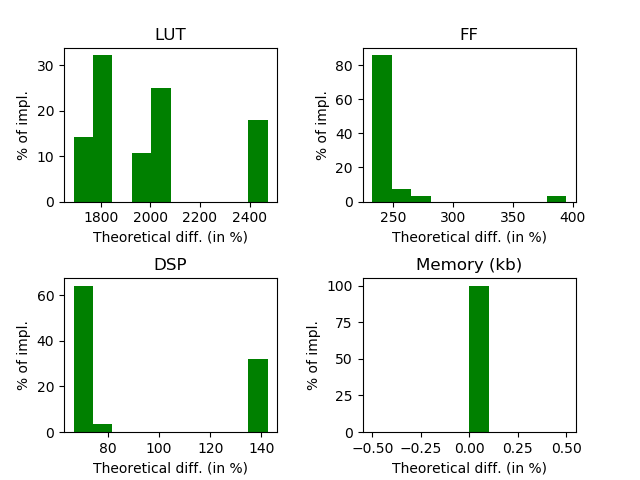
\includegraphics[width=.8\textwidth]{Figures/results/bsRelativeWithoutMacro}
        \caption{Without macro block replacement}
        \label{ch.expe:sec.estimators:ssec.resource:fig.bs:sfig.without}
    \end{subfigure}
    \begin{subfigure}{1.0\textwidth}
        \centering
        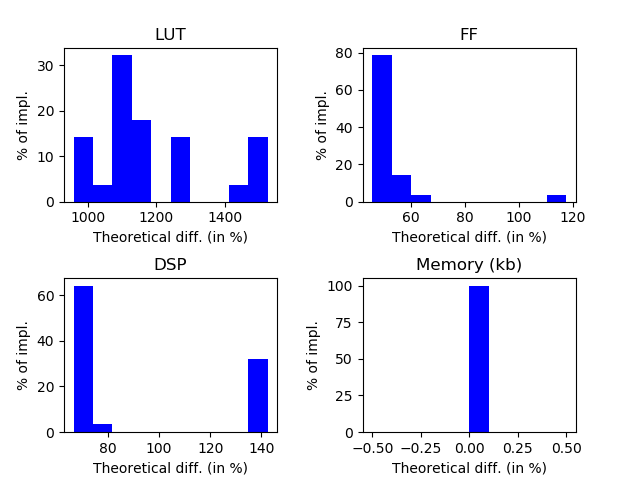
\includegraphics[width=.8\textwidth]{Figures/results/bsRelativeWithMacro}
        \caption{With macro block replacement}
        \label{ch.expe:sec.estimators:ssec.resource:fig.bs:sfig.with}
    \end{subfigure}
    \caption[Quality of resource estimation on Black Scholes]{Relative differences between the resource estimations\newline and the synthesis results on Black Scholes kernels}
    \label{ch.expe:sec.estimators:ssec.resource:fig.bs}
\end{figure}
\clearpage

\begin{figure}[h!]
    \centering
    \begin{subfigure}{1.0\textwidth}
        \centering
        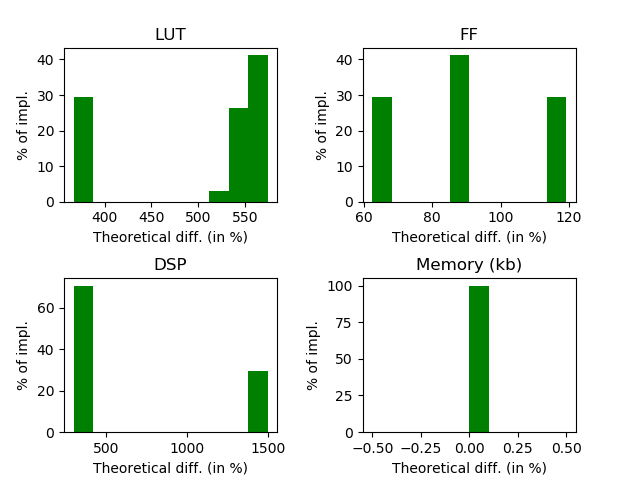
\includegraphics[width=.8\textwidth]{Figures/results/piRelativeWithoutMacro}
        \caption{Without macro block replacement}
        \label{ch.expe:sec.estimators:ssec.resource:fig.pi:sfig.without}
    \end{subfigure}
    \begin{subfigure}{1.0\textwidth}
        \centering
        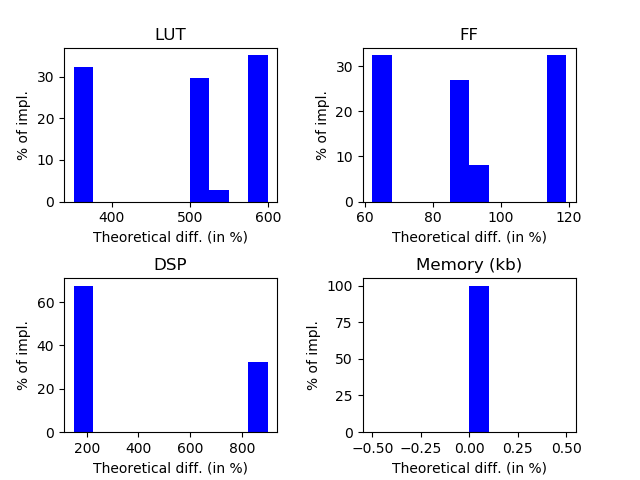
\includegraphics[width=.8\textwidth]{Figures/results/piRelativeWithMacro}
        \caption{With macro block replacement}
        \label{ch.expe:sec.estimators:ssec.resource:fig.pi:sfig.with}
    \end{subfigure}
    \caption[Quality of resource estimation on Pi]{Relative differences between the resource estimations\newline and the synthesis results on Pi kernels}
    \label{ch.expe:sec.estimators:ssec.resource:fig.pi}
\end{figure}
\clearpage

\begin{figure}[h!]
    \centering
    \begin{subfigure}{1.0\textwidth}
        \centering
        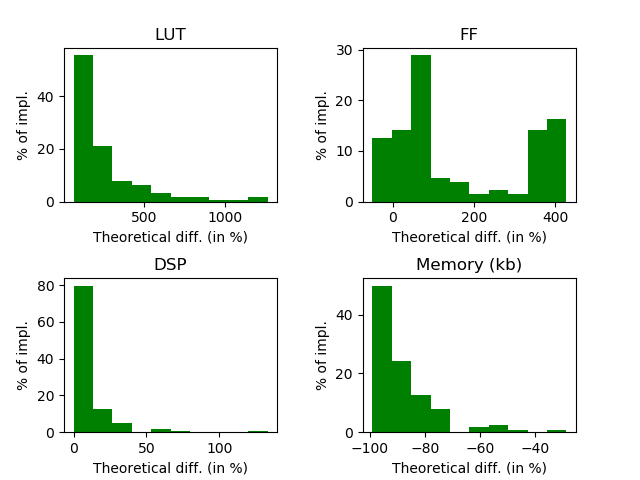
\includegraphics[width=.8\textwidth]{Figures/results/fftRelativeWithoutMacro}
        \caption{Without macro block replacement}
        \label{ch.expe:sec.estimators:ssec.resource:fig.fft:sfig.without}
    \end{subfigure}
    \begin{subfigure}{1.0\textwidth}
        \centering
        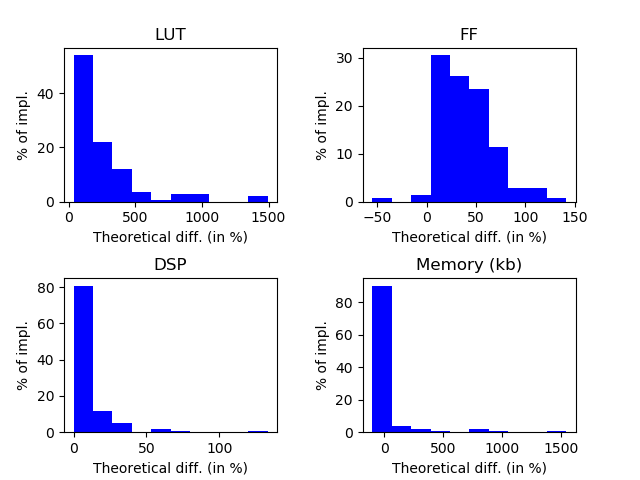
\includegraphics[width=.8\textwidth]{Figures/results/fftRelativeWithMacro}
        \caption{With macro block replacement}
        \label{ch.expe:sec.estimators:ssec.resource:fig.fft:sfig.with}
    \end{subfigure}
    \caption[Quality of resource estimation on FFT]{Relative differences between the resource estimations and\newline the synthesis results on Fast-Fourier Transform kernels}
    \label{ch.expe:sec.estimators:ssec.resource:fig.fft}
\end{figure}
\clearpage

\begin{figure}[h!]
    \centering
    \begin{subfigure}{1.0\textwidth}
        \centering
        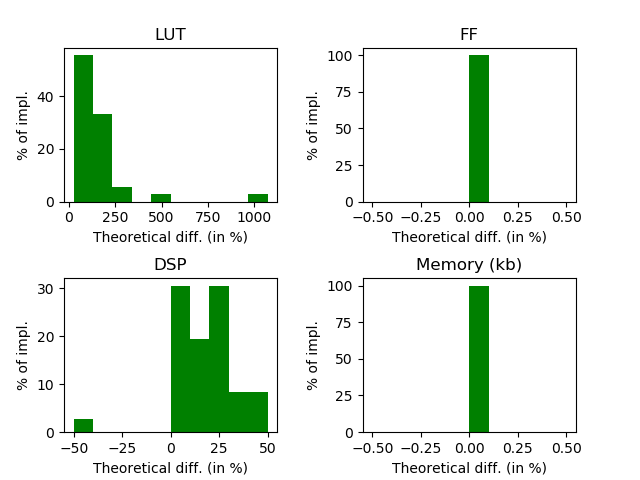
\includegraphics[width=.8\textwidth]{Figures/results/dpRelativeWithoutMacro}
        \caption{Without macro block replacement}
        \label{ch.expe:sec.estimators:ssec.resource:fig.dp:sfig.without}
    \end{subfigure}
    \begin{subfigure}{1.0\textwidth}
        \centering
        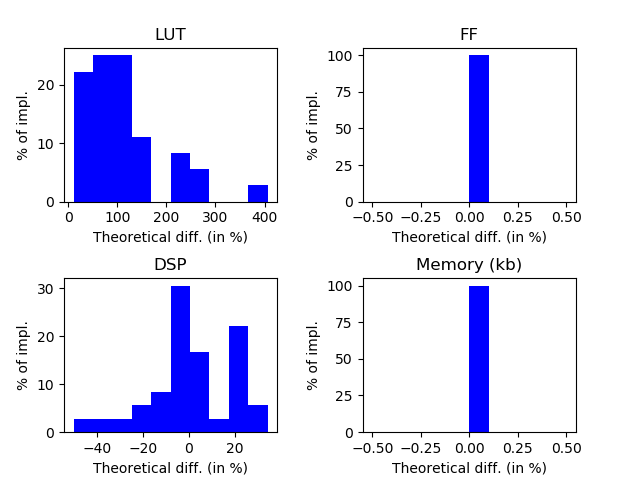
\includegraphics[width=.8\textwidth]{Figures/results/dpRelativeWithMacro}
        \caption{With macro block replacement}
        \label{ch.expe:sec.estimators:ssec.resource:fig.dp:sfig.with}
    \end{subfigure}
    \caption[Quality of resource estimation on dot product]{Relative differences between the resource estimations and\newline the synthesis results on dot product kernels}
    \label{ch.expe:sec.estimators:ssec.resource:fig.dp}
\end{figure}
\clearpage

\cleardoublepage
%-------------------------------------------------------------------------------
\chapter{Comparing the Pruning Strategies}
\labelchapter{app.quick}

%-------------------------------------------------------------------------------
This Appendix provides further data on the empirical \myLongAc{QoS}{Quality of Service} estimations that were introduced in Section \ref{ch.expe:sec.qece:ssec.impl}.
It shows the impact of the different pruning strategies for partitioning a given design space, with a particular focus on the quick pruning strategy that was defined in Algorithm \ref{ch.dse:sec.functional:ssec.basic:algo.quick}. 
For an easier representation of the results, we fix the {\it vector width} parameter to 8, as was done in Section \ref{ch.expe:sec.estimators:ssec.qos}.

In a similar way to what was done in Table \ref{ch.expe:sec.strategies:ssec.qos:table.quick}, we consider 4 different strategies for these experiments:
\begin{itemize}
    \item {\bf Strategy 1:} exhaustive pruning
    \item {\bf Strategy 2:} exhaustive pruning, with space reduction
    \item {\bf Strategy 3:} quick pruning, with space reduction (using \lstinline{SeqSpace})
    \item {\bf Strategy 4:} quick pruning, with space reduction (using \lstinline{MatrixSpace})
\end{itemize}

\vspace*{\fill}
\minilof

\clearpage

Table \ref{app.quick:table.strategies} introduces 8 different experiments for comparing those strategies --- see Table \ref{ch.expe:sec.strategies:ssec.qos:table.quick} for a detailed explanation of these experiments --- along with heat map representations of the \myAc{QoS} evolution.
For those experiments, we set the acceptable error threshold to 1\%, similarly to what was done in Figure \ref{ch.expe:sec.strategies:ssec.qos:fig.quick}.

As can be observed, the speed of the exhaustive strategies does not seem to be correlated with the initial distribution or with the number of simulations.
In fact, it seems that each simulation runtime is negligible with respect to the static cost of launching the simulator, resulting in a null gain when reducing the number of simulations.
However, as {\bf dot products} are quite simple kernels, it is possible that for more complex ones, the simulation runtime would scale, meaning that reducing the number of simulations could bring better performance.

On the other hand, we remark that changing the distribution (\ie the simulation workload) can have a direct impact on the number of implementations that are explored to build the {\bf pruning frontier}, thus impacting the duration of each strategy --- as the pruned space width reduces, it is easier to build that frontier and thus the pruning process becomes faster.
Moreover, we can use those results to confirm the impact that the space structures have on the exploration runtime.
We can remark that using a linear \lstinline{SeqSpace} can be more time-consuming than an exhaustive exploration of the space, while using a more complex \lstinline{MatrixSpace} implementation can result in an acceleration factor of $\times 5.4$, depending on the size of the pruned search space.

Finally, we can state that reducing the number of dimensions before the exploration is indeed an easy way to reduce the search time, under the assumtion that the user is aware that a particular dimension has no impact on a given metric for the considered exploration step.

As a conclusion, we can state that for \myAc{QoS}-based pruning, it seems to be better to use the {\bf quick pruning strategy} with a \lstinline{MatrixSpace} {\bf structure}, after performing {\bf space reduction}.\footnote{Here, only the {\it parallelism} dimension is being ignored at simulation time as it does not impact the implementations \myAc{QoS}. Moreover, as the {\it vector width} is fixed to 8, the exploration is thus in fact done in a {\bf two dimensional} space.}
One should also adapt the number of simulations in order to cope with the {\bf law of large numbers} and provide meaningful \myAc{QoS} results.

\clearpage

\begin{sidewaystable}[h!]
    \begin{tabular}{|c|cc|c|cc|cc|cc|cc|}
        \hline
        \multirow{2}*{{\bf \#}} & \multicolumn{2}{c|}{{\bf Distribution}} & {\bf Simulation} & \multicolumn{2}{|c|}{{\bf Strategy 1}} & \multicolumn{2}{|c|}{{\bf Strategy 2}} & \multicolumn{2}{|c|}{{\bf Strategy 3}} & \multicolumn{2}{c|}{{\bf Strategy 4}}\\
        ~ & Mean & Std dev. & {\bf number} & \#impl. & Time & \#impl. & Time & \#impl. & Time & \#impl. & Time\\
        \hline
        \ref{app.quick:fig.qos0-1-10} & 0 & 1 & 10 & 3844 & 12m26s & 961 & 3m08s & 275 & 5m23s & 275 & 54s\\ 
        \ccg \ref{app.quick:fig.qos0-1-50} & \ccg 0 &\ccg 1 & \ccg 50 & \ccg 3844 & \ccg 12m24s & \ccg 961 & \ccg 3m08s & \ccg 270 & \ccg 5m17s & \ccg 270 & \ccg 52s\\
        \ref{app.quick:fig.qos0-1-100} & 0 & 1 & 100 & 3844 & 12m22s & 961 & 3m09s & 260 & 5m06s & 260 & 49s\\
        \ccg \ref{app.quick:fig.qos0-1-1000} & \ccg 0 & \ccg 1 & \ccg 1000 & \ccg 3844 & \ccg 12m22s & \ccg 961 & \ccg 3m07s & \ccg 255 & \ccg 5m03s & \ccg 255 & \ccg 49s\\ 
        \ref{app.quick:fig.qos32-10-10} & 32 & 10 & 10 & 3844 & 12m24s & 961 & 3m09s & 181 & 3m23s & 181 & 35s\\ 
        \ccg \ref{app.quick:fig.qos32-10-50} & \ccg 32 &\ccg 10 & \ccg 50 & \ccg 3844 & \ccg 12m25s & \ccg 961 & \ccg 3m06s & \ccg 181 & \ccg 3m23s & \ccg 181 & \ccg 35s\\
        \ref{app.quick:fig.qos32-10-100} & 32 & 10 & 100 & 3844 & 12m32s & 961 & 3m08s & 181 & 3m24ss & 181 & 35s\\
        \ccg \ref{app.quick:fig.qos32-10-1000} & \ccg 32 & \ccg 10 & \ccg 1000 & \ccg 3844 & \ccg 12m20s & \ccg 961 & \ccg 3m07s & \ccg 181 & \ccg 3m25s & \ccg 181 & \ccg 35s\\ 
        \hline
    \end{tabular}
    \caption[Comparison of the pruning strategies on dot products]{Comparison of the pruning strategies on dot product implementations}
    \label{app.quick:table.strategies}
\end{sidewaystable}

\clearpage

\begin{figure}
    \centering
    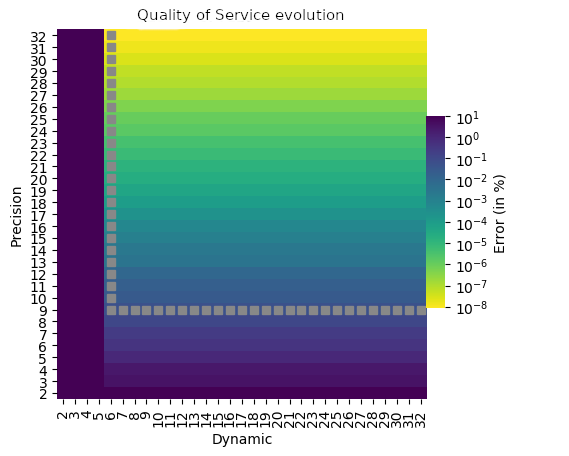
\includegraphics[width=.8\textwidth]{Figures/results/d2-32_p2-32_e8-8_N0-1_s10-0.png}
    \caption{Quality of service evolution ($\mathcal{N}(0, 1)$, 10 simulations)}
    \label{app.quick:fig.qos0-1-10}
\end{figure}
\begin{figure}
    \centering
    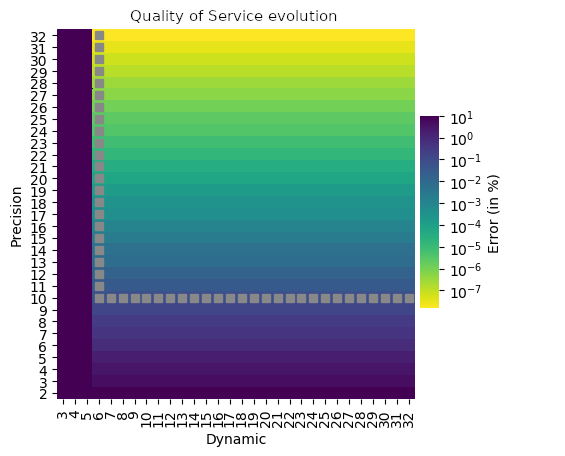
\includegraphics[width=.8\textwidth]{Figures/results/d2-32_p2-32_e8-8_N0-1_s50-0.png}
    \caption{Quality of service evolution ($\mathcal{N}(0, 1)$, 50 simulations)}
    \label{app.quick:fig.qos0-1-50}
\end{figure}
\begin{figure}
    \centering
    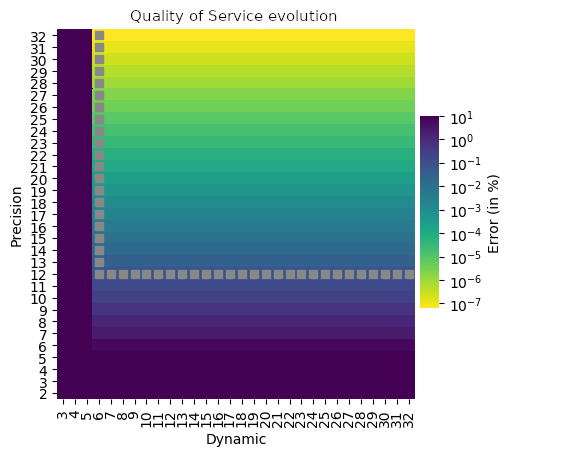
\includegraphics[width=.8\textwidth]{Figures/results/d2-32_p2-32_e8-8_N0-1_s100-0.png}
    \caption{Quality of service evolution ($\mathcal{N}(0, 1)$, 100 simulations)}
    \label{app.quick:fig.qos0-1-100}
\end{figure}
\begin{figure}
    \centering
    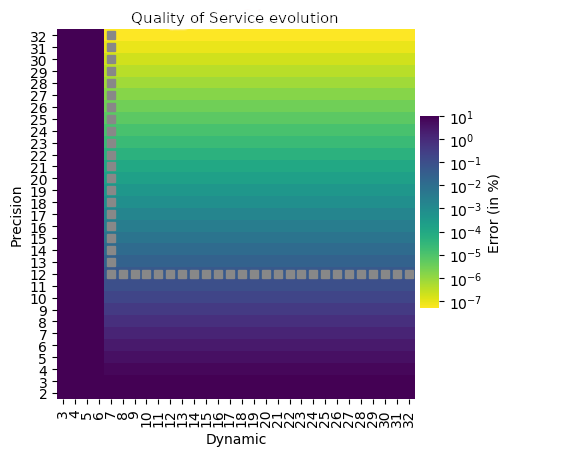
\includegraphics[width=.8\textwidth]{Figures/results/d2-32_p2-32_e8-8_N0-1_s1000-0.png}
    \caption{Quality of service evolution ($\mathcal{N}(0, 1)$, 1000 simulations)}
    \label{app.quick:fig.qos0-1-1000}
\end{figure}

\begin{figure}
    \centering
    \includegraphics[width=.8\textwidth]{Figures/results/d2-32_p2-32_e8-8_N32-10_s10-0.png}
    \caption{Quality of service evolution ($\mathcal{N}(32, 10)$, 10 simulations)}
    \label{app.quick:fig.qos32-10-10}
\end{figure}
\begin{figure}
    \centering
    \includegraphics[width=.8\textwidth]{Figures/results/d2-32_p2-32_e8-8_N32-10_s50-0.png}
    \caption{Quality of service evolution ($\mathcal{N}(32, 10)$, 50 simulations)}
    \label{app.quick:fig.qos32-10-50}
\end{figure}
\begin{figure}
    \centering
    \includegraphics[width=.8\textwidth]{Figures/results/d2-32_p2-32_e8-8_N32-10_s100-0.png}
    \caption{Quality of service evolution ($\mathcal{N}(32, 10)$, 100 simulations)}
    \label{app.quick:fig.qos32-10-100}
\end{figure}
\begin{figure}
    \centering
    \includegraphics[width=.8\textwidth]{Figures/results/d2-32_p2-32_e8-8_N32-10_s1000-0.png}
    \caption{Quality of service evolution ($\mathcal{N}(32, 10)$, 1000 simulations)}
    \label{app.quick:fig.qos32-10-1000}
\end{figure}



%---------------------------------------
% Backmatter : acronyms & biblio
%---------------------------------------
\backmatter
%---------------------------------------
\labelchapter{backmatter}
\addtocontents{toc}{\protect\contentsline{chapter}{Backmatter}{}{}}

%---------------------------------------
% Publications
%---------------------------------------
\pagestyle{empty}
\clearpage
\phantomsection
%-------------------------------------------------------------------------------
\chapter*{Publications}
\addcontentsline{toc}{chapter}{Publications}
\label{ch.publi}
\titleformat{\subsubsection}[runin]{\bfseries}{}{}{}[]

\newcommand{\publiSkip}[0]{2.5cm}
\newcommand{\publiEntry}[4]{%
     \noindent\mySub{\publiSkip}{#1}#2\hfill\cite{#3}\newline%
     \indent \emph{#4}\newline%
}
%-------------------------------------------------------------------------------

%%%%%%%%%%%%%%%%%%%%%%%%%%%%%%%%%%%%%%%%%%%%%%%%%%%%%%%%%%%%%%%%%%%%%%%%%%%%%%%%
%%%%%%%%%%%%%%%%%%%%%%%%%%%%%%%%%%%%%%%%%%%%%%%%%%%%%%%%%%%%%%%%%%%%%%%%%%%%%%%%

\section*{International publications}

\publiEntry{ARC2020}{Toledo, Spain (short paper + poster)}%
{ferres2020chisel}{Chisel Usecase: Designing General Matrix Multiply for FPGA}

\publiEntry{RSP'2021}{{\it Virtual event}}{ferres_2021_integrating}%
{Integrating Quick Resource Estimators in Hardware Construction Framework for Design Space Exploration}

% \section*{National publications}


%%%%%%%%%%%%%%%%%%%%%%%%%%%%%%%%%%%%%%%%%%%%%%%%%%%%%%%%%%%%%%%%%%%%%%%%%%%%%%%%
%%%%%%%%%%%%%%%%%%%%%%%%%%%%%%%%%%%%%%%%%%%%%%%%%%%%%%%%%%%%%%%%%%%%%%%%%%%%%%%%


%---------------------------------------
% Glossaire
%---------------------------------------
\clearpage
\phantomsection
%-------------------------------------------------------------------------------
\chapter*{Glossary}
\addcontentsline{toc}{chapter}{Glossary}
\label{ch.glossary}
%-------------------------------------------------------------------------------

%%%%%%%%%%%%%%%%%%%%%%%%%%%%%%%%%%%%%%%%%%%%%%%%%%%%%%%%%%%%%%%%%%%%%%%%%%%%%%%%
%%%%%%%%%%%%%%%%%%%%%%%%%%%%%%%%%%%%%%%%%%%%%%%%%%%%%%%%%%%%%%%%%%%%%%%%%%%%%%%%
%%%%%%%%%%%%%%%%%%%%%%%%%%%%%%%%%%%%%%%%%%%%%%%%%%%%%%%%%%%%%%%%%%%%%%%%%%%%%%%%

\newcommand{\extraentry}[1]{%
    .\newline\indent#1
}
\newcommand{\glossarySkip}[0]{2.5cm}

\DeclareDocumentCommand\glEntry{m m g}{%
    {\mySub{\glossarySkip}{#1}{\phantomsection\label{ch.glossary:gl.#1}{\it #2}%
        \IfNoValueF{#3}{\extraentry{#3.}}}%
    }\\[0.8cm]%
}

    \glEntry{API}{Application Programming Interface}{An interface proposed by the developers of programming tools to their users}
    \glEntry{AxC}{Approximate Computing}{Application domain relying on a simple assertion: most of the applications are redundant enough to allow approximation in the intermediate results, thus some resources can be saved by changing the data representation and using approximate \myAcs{FU}}
    \glEntry{ASIC}{Application-Specific Integrated Circuit}{An integrated circuit customized for a specific application}
    \glEntry{BOOM}{Berkeley Out-of-Order Machine}{A \chisel-based generator of RISC-V out-of-order cores \cite{celio_berkeley_2015}}
    \glEntry{BRAM}{Block Random-Access Memory}{A memory block embedded in the \myAc{FPGA} itself, allowing an access that is quicker than the external memories that may be available}
    \glEntry{Chisel}{Constructing Hardware in a Scala Embedded Language}{A \scala-based \myAc{HCL} developed at Berkeley since 2012 \cite{bachrach_chisel_2012}}
    \glEntry{CLB}{Configurable Logic Block}{Basic blocks for Xilinx \myAcs{FPGA}, including both computation resources (\myAcs{LUT}) and memory resources (\myAcs{FF})}
    \glEntry{CNN}{Convolutional Neural Network}{A neural network model where each neuron is connected to a bounded amount of preceding and succeeding neurons, in contrast to fully connected networks}
    \glEntry{CPU}{Central Processing Unit}
    \glEntry{DL}{Deep Learning}{Machine learning methods based on multiple layered networks}
    \glEntry{DIF}{Decimation In Frequency}{A standard approach for \myAc{FFT} computations, which enables consuming the temporal data in a \myAc{FIFO} fashion}
    \glEntry{DG}{Directed Graph}
    % \glEntry{DNN}{Deep Neural Network}
    \glEntry{DSE}{Design Space Exploration}{A manual or automatic methodology for the exploration of a design space, in order to find the best fit for an algorithm hardware implementation}
    \glEntry{DSL}{Domain Specific Language}{A programming language targeting a specific domain, and thus embedding very specific features which are keys for the usual computations in this field.
    \myAcs{DSL} can thus be accelerated using some specific components, and non experts can take advantage of such acceleration}
    \glEntry{DSP}{Digital Signal Processor}{A computing unit dedicated to digital processing applications}
    % \glEntry{DPR}{Dynamic Partial Reconfiguration}{Method used to reconfigure a part of the \myAc{FPGA} while it is running, without altering the run of the other parts}
    % \glEntry{FaaS}{FPGA as a Service}{Service offering access to one or many \myAc{FPGA} to users, which can program it with their custom designs.
    % It may include various levels of virtualization stacks, from a \tn{bare-metal} access to custom \tn{frameworks} for virtualization and resrouce sharing}
    \glEntry{FIFO}{First-In First-Out}{A data structure in which data are consumed in their order of arrival}
    \glEntry{FIR Filter}{Finite Impulse Response Filter}{A class of representative algorithms of signal processing.
    It is a digital filter using a finite number of coefficients}
    \glEntry{FIRRTL}{Flexible Intermediate Representation for \myAc{RTL}}{The \myLongAc{IR}{Intermediate Representation} used by \chisel}
\clearpage
    \glEntry{FF}{Flip Flop}{Basic units of memorization of one bit--- often assimilated to the registers}
    \glEntry{FFT}{Fast Fourier Transform}{A representative algorithm in the signal processing field. 
    It converts input data from the time domain to the frequency domain}
    \glEntry{FPGA}{Field-Programmable Gate Array}{A reconfigurable circuit that is able to behave as any sequential or combinatorial circuit}
    \glEntry{FPU}{Floating-Point Unit}{Computation units dedicated to floating-point computations, based on the IEEE-754 standard}
    \glEntry{FSM}{Finite State Machine}
    \glEntry{FU}{Functional Unit}{Computation units used as the basis of a given architecture}
    \glEntry{GA}{Genetic Algorithm}{A class of evolutionary algorithms that can be used for optimization and search problem resolution}
    \glEntry{GEMM}{General Matrix Multiply}{A representative algorithm in the field of linear algebra.
    It is a generalization of the basic matrix multiplication algorithm}
    \glEntry{GPU}{Graphical Processing Unit}
    \glEntry{HCF}{Hardware Construction Framework}{A framework used to compile an entry \myAc{HCL}-based code to a \myAc{RTL} description that can be fed to any low level toolchain.\\
    \myAcs{HCF} are similar to standard software compilers in their design, using a frontend/transforms/backend separation}
    \glEntry{HCL}{Hardware Construction Language}{A hardware language enabling the definition of hardware generators instead of hardware designs, to ease the re-utilization of the code, thus speeding-up the hardware development processes}
    \glEntry{HDL}{Hardware Description Language}{Standard \myAc{RTL} languages, such as \verilog{}, {\bf system-}\verilog{} or \vhdl}
    \glEntry{HLS}{High Level Synthesis}{A design methodology based on the compilation of algorithmic specification toward a hardware description, to ease and speed-up the hardware development}
    % \glEntry{HPC}{High Performance Computing}{Application domain dedicated to heavy computations}
    % \glEntry{HPC}{High Performance Computing}
    \glEntry{IO}{Input/Output}
    \glEntry{IR}{Intermediate Representation}{An internal representation used by a compiler to abstract concerns from both the entry language and the target machine}
    \glEntry{IP}{Intellectual Property (core)}{A reusable unit of logic, often subject to intellectual property laws, used as a functional block in \myAcs{ASIC} and \myAcs{FPGA}}
    \glEntry{JSON}{JavaScript Object Notation}{A JavaScript-based format for representing textual data}
    % \glEntry{LFSR}{Linear-Feedback Shift Register}{Digital component used to generate pseudo random number, using a shift register whose input is obtained by applying a linear function on its own output.}
    \glEntry{LUT}{Look-Up Table}{Basic electronic components, able to model any boolean function for a given amount of inputs (usually 4 or 6).
    Notably used in the design of recent \myAcs{FPGA}, due to this generic feature}
    \glEntry{MAC}{Multiply and Accumulate}{A basic pattern of operation used in many domains such as signal processing, image processing or machine learning.
    It relies on computing a joint addition and multiplication}
    \glEntry{ML}{Machine Learning}
    \glEntry{MLP}{Multilayer Perceptron}{A model of fully connected neural networks derived from the original Perceptron model \cite{rosenblatt1958perceptron}}
    \glEntry{MOP}{Multi-objective Optimization Problem}{As defined by Barone \etal{} \cite{barone_multi-objective_2021}, it is the process of "finding, for some {\it decision variables}, a set of values satisfying {\it imposed constraints}, while optimizing a set of {\it objective functions}" \cite{osyczka1985multicriteria}}
    \glEntry{NoC}{Network-on-Chip}{A design paradigm which aims at integrating the communication system directly on the chip}
    % \glEntry{OS}{Operating System}
    \glEntry{OOP}{Object-Oriented Programming}
    \glEntry{QECE}{Quick Exploration using Chisel Estimators}{An estimation and exploration framework built as a {\it proof of concept} of the usage of \myAcs{HCL} for \myAc{DSE} \cite{ferres_qece_2021}}
    \glEntry{QoR}{Quality of Results}{In the context of this thesis, we consider the \myAc{QoR} to be the quality of the proposed estimators with respect to some reference values about circuit properties.
    A distinction must be done between \myAc{QoR} and \myAc{QoS}, as the second one is an actual property of the circuit while the first one provides insights about the adequacy of the estimation flow with respect to the development environment}
    \glEntry{QoS}{Quality of Service}{A property of a circuit that exhibits the errors that were introduced by the implementation with respect to the initial algorithm.
    It is particularly relevant in the context of \myLongAc{AxC}{Approximate Computing}, where one can build more performant designs at the cost of accuracy}
    \glEntry{RAM}{Random-Access Memory}
    \glEntry{R2MDC}{Radix-2 Multi-Path Delay Commutator}{A standard technique for \myAc{FFT} optimization. 
    The proposed implementation is based on a presentation from Gerez \cite{gerez_fft_2012} (itself based on the literature \cite{rabiner1975theory})}
    \glEntry{RMSE}{Root-Mean-Square Error}{A standard metric defined by computing the relative differences between theoretical and experimental values}
    \glEntry{RTL}{Register-Transfer Level}{The abstraction level used for hardware development, abstracting low level consideration to only consider signal interactions}
    \glEntry{ROM}{Read-Only Memory}
    \glEntry{SoC}{Systems on a Chip}{A single integrated circuit (\myAc{ASIC}) embedding all the needed components - such as memories, \myAc{IO} ports or microprocessors - for a given application}
    \glEntry{TPU}{Tensor Processing Unit}{An Artificial Intelligence dedicated \myAc{ASIC}}
    \glEntry{VLSI}{Very Large Scale Integration}{Design processes used to integrate millions of transistors in a chip}

%%%%%%%%%%%%%%%%%%%%%%%%%%%%%%%%%%%%%%%%%%%%%%%%%%%%%%%%%%%%%%%%%%%%%%%%%%%%%%%%
%%%%%%%%%%%%%%%%%%%%%%%%%%%%%%%%%%%%%%%%%%%%%%%%%%%%%%%%%%%%%%%%%%%%%%%%%%%%%%%%

%%%%%%%%%%%%%%%%%%%%%%%%%%%%%%%%%%%%%%%%%%%%%%%%%%%%%%%%%%%%%%%%%%%%%%%%%%%%%%%%


%---------------------------------------
% References
%---------------------------------------
\cleardoublepage
\phantomsection
\addcontentsline{toc}{chapter}{Bibliography}
\interlinepenalty=10000
\Urlmuskip=0mu plus 1mu\relax
% a custom bibstyle is available, however I don't like it
% \bibliographystyle{StyleThese}
\bibliographystyle{alpha}
\bibliography{thesis}


%---------------------------------------
% Back Page
%---------------------------------------
\finalpage{\phantomsection
\pdfbookmark[0]{Back page}{backpage}
\renewcommand*{\hrulefill}[1][-0.2mm]{\leavevmode \leaders \hrule height #1 \hfill \kern 0pt}

% /!\ Careful with this, it's hand tuned...
\changepage{7em}{9em}{-7em}{-4em}{-10em}{-5em}{}{}{}
%---------------------------------------

%---------------------------------------
% English
%---------------------------------------

% \section*{TITLE}
\noindent{\Large\bf Leveraging Hardware Construction Languages for Flexible Design Space Exploration on FPGA}

\vspace*{\fill}
% \section*{SUMMARY}
{\normalsize
\noindent{\bf Abstract} --- FPGA based accelerators are imposing themselves as energy efficient alternatives to general purpose CPUs.
However, the hardware development methodologies are still way behind their software counterparts, and initiatives are to be taken in order to increase the productivity of hardware developers.
In this thesis, we explore the possibilities that the emerging Hardware Construction Languages paradigm can bring to the hardware world, notably by leveraging high level features such as functional programming or object oriented development.
We start with a comprehensive analysis of the estimation metrics and methodologies in the context of FPGA development, and then put a particular focus on how such paradigm can be used for design space exploration, introducing two complementary methodologies --- {\it meta design} and {\it meta exploration} --- for such usage.
A software demonstrator, QECE, has been developed and used to demonstrate the usability of those methodologies in various use cases, thanks to a custom benchmark made  of representative applicative kernels.

This thesis is an initiative to enhance hardware developers expressivity, providing them with powerful features such as functional programming and object-oriented development.
}
\vspace*{\fill}%

% \section*{KEYWORDS}
\noindent{\normalsize\it {\bf Keywords:} FPGA, hardware accelerators, Chisel, design space exploration}
~\\

%---------------------------------------
% \hrulefill[1pt]
\vspace{-0.25cm}
\hrule height 1pt
\vspace{0.3cm}
%---------------------------------------

%---------------------------------------
% Français
%---------------------------------------

% \section*{TITRE}
\noindent{\Large\bf Utilisation de langages de construction mat\'erielle pour une exploration flexible des espaces de conception sur FPGA}

\vspace*{\fill}
% \section*{R\'ESUM\'E}
{\normalsize
\noindent{\bf R\'esum\'e} --- Les accélérateurs matériels à base de FPGA s'imposent actuellement comme une alternative à haute efficacité énergétique aux processeurs généralistes classiques.
Cependant, les méthodologies de développement matériel souffrent d'un grand retard par rapport à leurs pendants logiciels, et des initiatives sont nécessaires afin d'accroire la productivité des concepteurs matériels.
Dans cette thèse, nous explorons les possibilités que les nouveaux langages de construction matérielle ouvrent pour le monde de la conception numérique, notamment en permettant l'usage de fonctionnalités de haut niveau telles que la programmation fonctionnelle ou le développement orienté objet.
Nous proposons tout d'abord une analyse de différentes métriques et méthodologies d'estimation pour le développement sur FPGA, et nous intéressons ensuite plus particulièrement à ce que ces nouveaux langages peuvent apporter au domaine de l'exploration d'espace de conception, en introduisant deux méthodologies complémentaires: la {\it méta conception} et la {\it méta exploration}.
Un logiciel démonstrateur, nommé QECE, est développé et utilisé afin de démontrer l'utilisabilité de ces méthodologies sur différents cas d'utilisation, gr\^ace à un ensemble de noyaux applicatifs que nous avons développés.

Cette thèse est une initiative pour améliorer l'expressivité des développeurs matériels, en leur fournissant des fonctionnalités à fort potentiel telles que la programmation fonctionnelle ou le développement orienté objet.
}
\vspace*{\fill}%

% \section*{MOTS-CL\'ES}
\noindent{\normalsize\it {\bf Mots-cl\'es:} FPGA, acc\'el\'erateurs mat\'eriel, Chisel, exploration d'espace de conception}
~\\

%---------------------------------------
% \hrulefill[3pt]
%---------------------------------------

% \section*{ISBN: }
\centering
Thesis prepared at TIMA laboratory

46 Avenue F\'elix Viallet, 38031, GRENOBLE Cedex, France

% {\bf ISBN:}
% \vspace{-6em}
\vspace{-4em}

%---------------------------------------
}
\let\clearpage\relax

%---------------------------------------
\end{document}

